\documentclass[11pt,letterpaper,oneside,openright]{book}


% tipo de letra Helvetica, algo parecida a Arial
% \usepackage{helvet}
% \renewcommand{\familydefault}{\sfdefault}


\usepackage[spanish]{babel}
\usepackage[utf8]{inputenc}
\usepackage{lmodern}
\usepackage[T1]{fontenc}
\usepackage[dvipsnames]{xcolor}

\usepackage{textcomp}
\usepackage[pdftex]{hyperref}
\usepackage{multirow}
\usepackage{booktabs}

% \usepackage{multirow}
\usepackage{amsmath}
\usepackage{microtype}


\usepackage{graphicx}
\usepackage{tikz}
\usepackage{pgfgantt}
\usepackage{pgfkeys}
\usepackage{float}
% \usepackage{minted}

\usepackage{svg}
\usepackage{amsmath}
% \usepackage{listings}

%para codigo fuente
\usepackage{color}
\usepackage{xcolor}
\usepackage{listings}

%Bibliografia en el indice
%\usepackage[nottoc,numbib]{tocbibind}
\usepackage[nottoc,notlot,notlof]{tocbibind}
%para bookmarks

%para numerar subsubsections
\setcounter{secnumdepth}{3}
%\setcounter{tocdepth}{3}
%menos profundidad en el indice
\setcounter{tocdepth}{1}


\usepackage{tabularx}
\usepackage{array}
\renewcommand{\tabularxcolumn}[1]{>{\small}m{#1}}

\newcolumntype{L}[1]{>{\raggedright\let\newline\\\arraybackslash\hspace{0pt}}m{#1}}
% \newcolumntype{X}[1]{>{\raggedright\let\newline\\\arraybackslash\hspace{0pt}}m{#1}}

\newcolumntype{R}[1]{>{\raggedleft\let\newline\\\arraybackslash\hspace{0pt}}m{#1}}
\newcolumntype{C}[1]{>{\centering\let\newline\\\arraybackslash\hspace{0pt}}m{#1}}

% \usepackage{xcolor}
% \usepackage{bordermatrix}
% \usepackage{microtype}
% \usepackage{shortvrb}
% \usepackage{tabularx}
%%%%%%%%%%%%%%%%%
% PARA HACER LA PRUEBA
%%%%%%%%%%%%%%%%%
% \usepackage{nicefrac}
% \usepackage[pdftex]{hyperref}
% \usepackage{anysize}
% \usepackage{fancyhdr}
% \usepackage{subfigure}
% \usepackage{pstricks}
% \usepackage{tabulary}
% \usepackage{type1cm}
% \usepackage{url}
% \usepackage{multirow}
% \usepackage{booktabs}
% \usepackage{subfigure}
% \usepackage{graphicx}
% \usepackage{bm}
%%%%%%%%%%%%%%%%%%%%%%%%%%%%%%%%%%%%%%
% \usepackage[bookmarks]{}
% \usepackage[bookmarks,colorlinks]{hyperref}
\graphicspath{{images/}}
\setsvg{
    svgpath = images/,
    inkscape = inkscape -z -D % conversion options for svg package, export drawing instead of page
}
% \renewcommand{\arraystretch}{1.5}
% \usepackage{hyperref}
\hypersetup{colorlinks,%
            citecolor=black,%
            filecolor=black,%
            linkcolor=black,%
            urlcolor=black}

% \usepackage[charter]{mathdesign}

%----------------------------------------
\usepackage{bookmark}
\bookmarksetup{numbered}

\usepackage{titlesec} %reformatting the chapter headings
%\titleformat{\chapter}[block]
%  {\normalfont\LARGE\bfseries\centering}
%  {CHAPTER\thechapter: }{0em}{}

% \makeatletter
% \bookmarksetup{%
%   addtohook={%
%     \ifnum\toclevel@chapter=\bookmarkget{level}\relax
%       \renewcommand*{\numberline}[1]{Cap\'itulo #1: }%
%     \fi
%   },
% }
% \makeatother
%----------------------------------------


%-----------------------------
\renewcommand{\lstlistingname}{Code}

\lstset{
    basicstyle=\footnotesize\ttfamily,
    language=C++
}
\usepackage{caption}
\DeclareCaptionFont{white}{\color{white}}
\DeclareCaptionFormat{listing}{\colorbox{gray}{\parbox{\textwidth}{#1#2#3}}}
\captionsetup[lstlisting]{format=listing,labelfont=white,textfont=white}
%-------------

%margenes

%segun guia
% \usepackage[top=2cm, bottom=2cm, inner=3cm, outer=2cm]{geometry}

%segun CD de carrera
\usepackage[top=2.5cm, bottom=2.5cm, inner=3.5cm, outer=2.5cm]{geometry}

% quita la sangria a los parrafos (sin sangria se ve feo :-)
%\setlength{\parindent}{0cm}

% Para tener cabecera y pie de pagina con un estilo personalizado
\usepackage{fancyhdr}
% \usepackage{floatpag}

\pagestyle{fancy}
\fancyhf{}% Clear page header/footer
\renewcommand{\headrulewidth}{0pt}% No header rule
\fancyfoot[C]{\thepage}
\floatpagestyle{fancy}% Page style for float-page only

%------------

% Espacio parrafos
\setlength{\parskip}{6pt}

\usepackage[pdftex]{graphicx}
\pdfcompresslevel=9

\usepackage{adjustbox}

%-------------------------------

%
% caratula
%
%para poner bookmark del CD de requisitos
\bookmark[page=1,level=-2]{INICIO}

\pagenumbering{Roman} % para comenzar la numeracion de paginas en numeros romanos


% \title{Desarrollo de una aplicaci\'on web móvil para visitas dentro el campus de la UMSS usando Geolocalización}
% \author{Edmundo Figueroa Herbas}
% \date{\today \ }

% caratula --------------------------------------------------------------
\newcommand{\umsslogo}{%
      \adjustbox{valign=t}{
\includegraphics[scale=0.04]{umss}}%
}
\newcommand{\fcytlogo}{%
      \adjustbox{valign=t}{
\includegraphics[scale=0.1]{fcyt}}%
}

% Car�tula:
\begin{titlepage}
\thispagestyle{empty}

\begin{tabular}[t]{c p{10cm} c}
    \umsslogo &
    \begin{center}
    \large{\textsc{Universidad Mayor de San Sim\'on }} \\
    \large{\textsc{Facultad de Ciencias y Tecnolog\'ia }} \\
    \large{\textsc{Carrera de Ingenier\'ia de Sistemas}}
    \end{center}
    &
    \fcytlogo \\
\end{tabular}
\vfill

\begin{center}
\huge{\textsc{Desarrollo de una aplicaci\'on web móvil para visitas dentro el campus de la UMSS usando Geolocalización}}
\end{center}
\vspace{0.5cm}

% \title{Desarrollo de una aplicaci\'on web móvil para visitas dentro el campus de la UMSS usando Geolocalización}
% \author{Edmundo Figueroa Herbas}
% \date{\today \ }

%\begin{flushright}
\begin{center}
\textsc{
Proyecto de grado, presentado para optar\\
al Diploma Académico de Licenciatura \\
en Ingeniería de Sistemas.
}
%\end{flushright}
\end{center}

\vfill
\begin{tabbing}
\hspace{2cm}\=\+
	\textsc{Presentado por:} Edmundo Figueroa Herbas	\\
    \\
	\textsc{Tutor:} Ing. Carlos Alberto Gomez Ormachea	\\
    \\
	%\textsc{Cochabamba - Bolivia}\\
    \\
\end{tabbing}

\begin{center}
    \textsc{Cochabamba - Bolivia}\\
    \textsc{Abril, 2017}
\end{center}

\vfill

%\hrule
%\vspace{0.2cm}
%\noindent\small{Trabajo de Grado \hfill}

\end{titlepage}

% caratula --------------------------------------------------------------




\begin{document}
% \include{title-page}
\frontmatter
  % \maketitle
  \tableofcontents

\mainmatter{}
  \chapter{Introducción} % (fold)
\label{cha:introduccion}

El presente proyecto consiste en el desarrollo de una aplicación móvil que permita ubicar y encontrar una locación dentro del campus de la Universidad Mayor de San Simón, la aplicación deberá localizar la ubicación actual del usuario y permitir especificar un punto de destino, mostrando a continuación el camino más corto para llegar a destino.

El campus universitario abarca más de 214,000 $m^2$ y encierra varias facultades y oficinas administrativas, para estudiantes nuevos y antiguos o personas que
necesitan hacer trámites administrativos, incluso si solo se quiere conocer el
campus, es necesario contar con un mapa donde ubicarse.

Las aplicaciones móviles tienen una gran demanda por parte de la población ya
que la gran mayoría posee un \emph{smartphone} o teléfono inteligente con capacidad de
ejecutar aplicaciones muy fácilmente, los \emph{smartphones} cuentan también con GPS,
el cual se usa para conocer la ubicación del usuario con un margen de error de
3 metros, usando puntos de referencia geo-localizados se puede determinar la
ruta óptima para llegar a destino. Es una desventaja para nuestra Universidad que no exista información confiable de fácil acceso para poder desplazarse por el campus.

  \section{Antecedentes} % (fold)
  \label{sec:antecedentes}

  Actualmente \emph{Google Maps} ofrece una solución al problema de encontrar una ruta entre 2 puntos geolocalizados, ya que sugiere posibles rutas si se usara movilidad, bicicleta o para ir caminando, para lograr esto se toman en cuenta los distintos tipos de calles que existen y la dirección en el caso de movilidades, \emph{Google Maps} toma en cuenta la descripción de una locación o la referencia cartográfica en latitud y longitud de los puntos, y el cómo se va a desplazar entre los 2 puntos para dibujar con una línea roja la ruta a seguir.

  Así como también existen Blogs o Aplicaciones con información de los lugares turísticos o de interés para visitar en la ciudad, como ser TripAdvisor, la información que provee esta aplicación generalmente incluye la locación del lugar referenciada sobre un mapa estático, este tipo de aplicaciones usa el API de \emph{Google Maps} para lograr encontrar una ruta hacia el lugar de interés.

  En el caso del campus de la Universidad Mayor de San Simón, Google Maps no cuenta con la información para lograr este objetivo, de encontrar una ruta entre 2 puntos geo-referenciados, ya que se necesita de un mapa de los caminos internos del campus Universitario e información de las aulas, kioscos, fotocopiadoras, oficinas, etc. Esta información no está disponible o es de difícil acceso lo cual genera malestar cuando se busca una locación dentro del campus Universitario.

  \section{Descripción del problema} % (fold)
  \label{sec:desc_probl}

  % Al andar dentro del campus universitario buscando algún lugar o punto de interés, es generalmente de gran prioridad reducir el tiempo en el cual se llega al aula u oficina, lamentablemente el campus Universitario carece de un buen sistema de señalización por lo que para llegar al punto de destino es necesario preguntar la  la Universidad hacia gente externa que necesitan hacer uso o encontrar algún lugar en especifico ya que lamentablemente esta información actualmente sólo te la pueden ofrecer las personas que conocen el lugar de antemano y aun en esos casos existe la posibilidad de no encontrar el lugar que se está buscando.\\

  La Universidad Mayor de San Simón no cuenta con un mapa interactivo que
  muestre la ubicación de los puntos o lugares que se encuentran dentro del
  campus universitario y como llegar hasta su ubicación, la falta de señalización obstaculiza el desplazamiento de los estudiantes o personas que requieren encontrar alguna oficina para, por ejemplo, realizar trámites administrativos, encontrar aulas o auditorios, etc. como resultado se pierde tiempo al tratar de encontrarlos por lo que un mapa con estas características sería de gran ayuda para el desplazamiento dentro del campus universitario. En la figura  \ref{fig:arbolProblemas}, se puede apreciar al árbol de problemas.

  % \begin{figure}[!hbp]
  %   \centering
  %   \includesvg{arbolProblemas}
  %   \caption{Diagrama Árbol de Problemas}
  %   \label{fig:arbolProblemas}
  % \end{figure}


  \begin{figure}[H]
    \begin{center}
      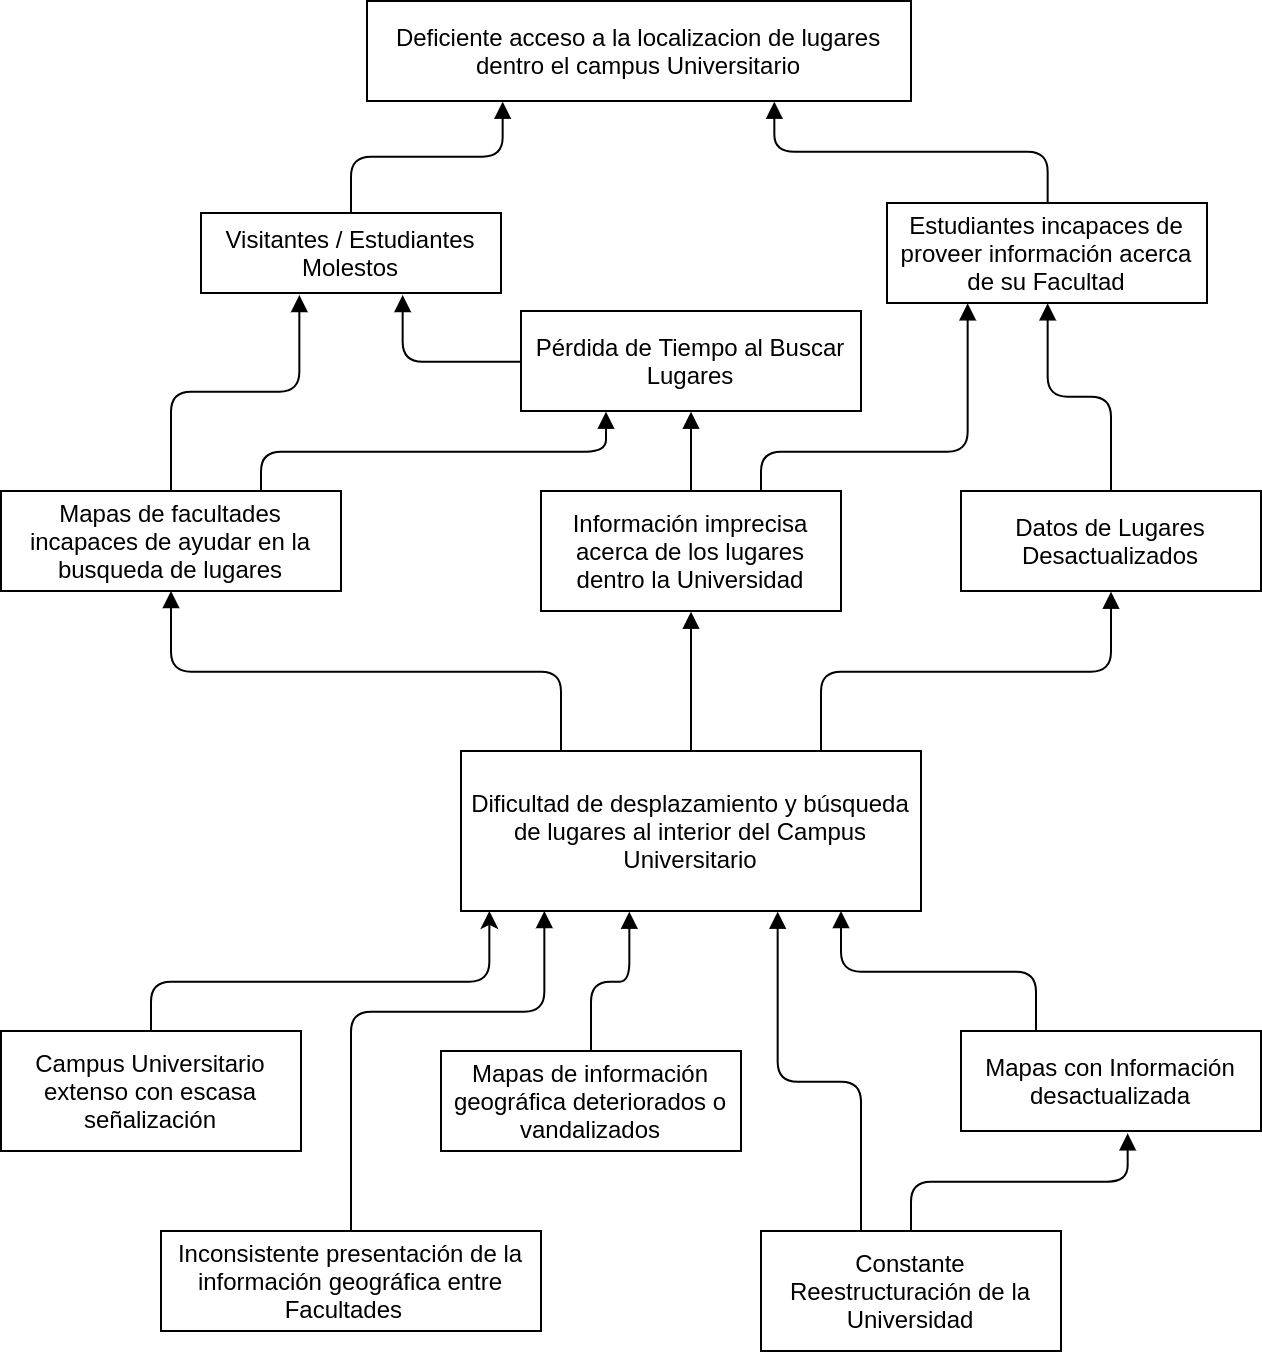
\includegraphics[width=0.65\textwidth]{diagramas/arbolProblemas}
    \end{center}
    \caption{Diagrama Árbol de Problemas}
    \label{fig:arbolProblemas}
    \caption*{Fuente: Elaboración propia}
  \end{figure}

  \section{Objetivo general} % (fold)
  \label{sec:objetivo_general}
    \begin{quote}
      Desarrollar una aplicación web móvil \emph{responsive} para optimizar la búsqueda de lugares y el  desplazamiento al interior del Campus Universitario de la UMSS.
    \end{quote}
  % section objetivo_general (end)


  \section{Objetivos Específicos} % (fold)
  \label{sec:obj_especificos}
    \begin{itemize}
      \item Generar un mapa con información geográfica de las rutas dentro del campus Universitario.
      \item Administrar lugares geolocalizados dentro del campus Universitario.
      \item Mostrar en la aplicación los lugares geolocalizados desplegando la ruta óptima desde mi posición hasta el punto destino.
      \item Administrar usuarios en el sistema.
      \item Registrar las búsquedas sobre rutas realizadas por los usuarios en el sistema.
    \end{itemize}
  % section obj_especificos (end)


  \section{Justificación} % (fold)
  \label{sec:justificacion}

  El Campus Universitario es bastante extenso y se encuentra en constante reestructuración, debido a que las aulas se incrementan, las oficinas son reubicadas, etc. gracias a esto es que los mapas con los que cuenta cada facultad, que son escasos y están impresos sobre banners estáticos, son también difíciles de actualizar. Este hecho genera malestar en estudiantes que llegan tarde a sus clases o necesitan llegar a algún Auditorio o personas/visitantes en proceso de realizar trámites administrativos, no encuentran con facilidad las oficinas a las que necesitan llegar.

  Una aplicación que permita localizar o encontrar locaciones y además proveer la ruta óptima dentro del campus de la Universidad Mayor de San Simón es de gran importancia para brindar apoyo a cualquier persona que necesite desplazarse por el campus Universitario.

  Las Aplicaciones móviles y/o web demostraron ser el futuro del desarrollo de software y la gran mayoría de los países en el mundo consumen estas soluciones y es necesario apuntar a esta tendencia.


  % section justificacion (end)
% chapter introduccion (end)

  \section{Alcance}
  \label{sec:Alcance}

    \subsection{Alcance Práctico}
    \label{sub:alcance_practico}

    Una aplicación web móvil puede llegar a ser muy compleja y manejar información sensible, y ya que el servidor está expuesto al acceso público de los usuarios, es susceptible de ataques maliciosos y malintencionados para acceder y robar información privada que los usuarios podrían tener almacenados en la aplicación, en el caso de la presente aplicación, el sistema no manejará información sensible del usuario, como ser tarjetas de crédito pero la aplicación manejará información de lugares, información que podría ser corrompida por usuarios malintencionados. La seguridad es muy importante para una aplicación web, por lo cual el presente proyecto implementara medidas de seguridad para asegurar la identidad del usuario que está solicitando el ingreso al sistema pero no incluirá protección a ataques Phishing, DoS ya que los objetivos específicos no los contempla.\\


    El \emph{look and feel} de una aplicación web es un tema muy importante para cualquier aplicación a desarrollar, para lograr que la aplicación se muestre de manera consistente en la pantalla de un smartphone se usarán herramientas de terceros pero no se extenderá el uso de la misma para la pantalla de un ordenador de escritorio que posee una resolución de pantalla muy superior al de un celular.\\



    % end alcance_practico

    \subsection{Alcance Metodológico}
    \label{sub:alcance_metodologico}
    Para la conclusión exitosa del presente proyecto se implementará la metodología  Programación Extrema (XP) y cada iteración del proceso tiene como meta el desarrollo conjunto de diferentes módulos, historias de usuario y la documentación relacionada.
    % end alcance_metodologico

    \subsection{Alcance Teórico}
    \label{sub:alcance_teorico}
    La investigación se limita a las estructuras, herramientas y estándares actuales sugeridos en la documentación y bibliografía consultada para la construcción de una aplicación web móvil.
    % end alcance_teorico

  % end Alcance






% Metodología:
% Agile Unified Process (AUP) es una versión simplificada de Rational  Proceso
% Unificado  (RUP).

% Fases del ciclo de desarrollo
%   Principio: El objetivo es  identificar el alcance inicial del proyecto y una
%   arquitectura potencial del sistema.

%   Elaboración: El objetivo es confirmar la idoneidad de la arquitectura del sistema.
%   Construcción: El objetivo es desarrollar software funcional dentro de un sistema regular e incremental periódicamente que mire las necesidades de las partes interesadas.
%   Transición: El objetivo es validar y desplegar el sistema en su entorno de producción.
% Las disciplinas del ciclo de desarrollo se llevan de manera iterativa y son
% las siguientes
%   Modelo: El objetivo de esta disciplina es entender el negocio de la organización, el dominio del problema que se ocupa el proyecto, y determinar una solución viable para hacer frente al dominio del problema.
%   Aplicación: El objetivo de esta disciplina es transformar el modelo de su (s) en el código ejecutable y para llevar a cabo un nivel básico de las pruebas, en las pruebas de unidad en particular.
%   Prueba: El objetivo de esta disciplina consiste en realizar una evaluación objetiva para asegurar la calidad. Esto incluye encontrar defectos, validar que el sistema funcione como está previsto, y verificar que se cumplan los requisitos.
%   Implementación: El objetivo de esta disciplina es el plan para la entrega del sistema y para ejecutar el plan para que el sistema a disposición de los usuarios finales.
%   Gestión de la Configuración: El objetivo de esta disciplina consiste en administrar el acceso a artefactos de su proyecto. Esto incluye no sólo el seguimiento de versiones de los artefactos a través del tiempo, sino también el control y la gestión de los cambios a los mismos.
%   Gestión de Proyectos: El objetivo de esta disciplina es dirigir las actividades que lleva a cabo en el proyecto. Esto incluye la gestión de riesgos, la dirección de personas (la asignación de tareas, seguimiento de los progresos, etc.), y coordinar con la gente y los sistemas fuera del alcance del proyecto para asegurarse de que se entregue a tiempo y dentro del presupuesto.
%   Para el Medio Ambiente: El objetivo de esta disciplina es apoyar el resto de los esfuerzos por garantizar que el proceso, la orientación adecuada (las normas y directrices), y herramientas (hardware, software, etc.) están disponibles para el equipo según sea necesario.
% % Fig. Ciclo de vida del Proceso Unificado Ágil

  \chapter{Marco Teorico} % (fold)
\label{cha:marco_teorico}

La aplicación a desarrollar estará enfocado a su uso en un celular inteligente (smartphone) por lo que hay que determinar el enfoque de desarrollo que se usará y las herramientas necesarias para construir esta aplicación.

\section{Aplicaciones Móviles}
\label{sec:aplicaciones_moviles}

  El desarrollo de aplicaciones web se divide en 3 grupos de enfoques de desarrollo.\\

  \subsection{Aplicaciones Nativas}
  \label{sub:aplicaciones_nativas}

  Las aplicaciones nativas se caracterizan de poder acceder directamente al sistema operativo móvil sin ningún intermediario ni contenedor.\\

  La aplicación nativa puede acceder libremente a todas las APIs (\emph{Application Program Interface} es un conjunto de herramientas, protocolos y rutinas que son usados para desarrollar aplicaciones, un API específica como tienen que interactuar los componentes de un sistema.) que el proveedor del Sistema Operativo (SO) ponga a disposición y, en muchos casos, tiene características y funciones únicas que son típicas del SO móvil en particular.\\

  Este tipo de aplicaciones se adapta al 100\% con las funcionalidades y características del dispositivo obteniendo así una mejor experiencia de uso.\\

  % end aplicaciones_nativas

  \subsection{Aplicaciones Web}
  \label{sub:aplicaciones_web}

  Los dispositivos móviles modernos pueden ejecutar navegadores con capacidad de ejecutar HTML5 (\emph{Hiper Text Markup Language} el cual es el lenguaje para escribir páginas Web), la cual es la Versión de HTML publicado en Octubre 2014, es la más moderna y en la que se escriben todas las aplicaciones web actuales, así como también incorporan un motor JavaScript que permite ejecutar código para lograr una página Web dinámica. Algunos ejemplos del potencial de HTML5 son: componentes IU avanzados, acceso a múltiples tipos de medios, servicios de geoposicionamiento y disponibilidad offline. Al emplear estas características se puede crear aplicaciones avanzadas usando únicamente tecnologías basadas en la Web.\\

  Se debe distinguir entre las aplicaciones Web, las aplicaciones Web diseñadas para dispositivos móviles ya que estas últimas reconocen cuando se accede a través de un smartphone y despliegan una página HTML que fue diseñada para brindar una experiencia táctil y cómoda en una pantalla pequeña, a este diseño de aplicación se le conoce como aplicación web responsive, esto mejora la experiencia del usuario creando un sitio Web móvil que se parezca a una aplicación nativa.\\

  % end aplicaciones_web

  \subsection{Aplicaciones Híbridas}
  \label{sub:aplicaciones_hibridas}

    El enfoque híbrido combina desarrollo nativo con tecnología Web. Usando este enfoque, se escribe gran parte de la aplicación usando tecnologías Web y se mantienen el acceso directo a APIs nativas cuando se necesita. La porción nativa de la aplicación emplea APIs del sistemas operativo para crear un motor de búsqueda HTML incorporado que funciona como un puente entre el navegador y las APIs del dispositivo\cite{IBM_Mobile}.\\

    Esto permite que la aplicación híbrida aproveche todas las características que ofrecen los smartphones modernos. Para lograr esto existen bibliotecas tal como Apache Cordova (antiguamente conocido como \textbf{PhoneGap}, es una de las herramientas más populares para crear aplicaciones híbridas.) que provee una interfaz JavaScript con funcionalidad para conectarse con los dispositivos seleccionados y lograr manejar el API propio del smartphone.\\

    La porción Web de la aplicación puede ser una página Web que resida en un servidor o bien un conjunto de archivos HTML, JavaScript, CSS y contenido multimedia, incorporados en el código de la aplicación y almacenados localmente en el dispositivo\cite{IBM_Mobile}.\\

  % Una mayor fragmentación de dispositivos móviles y tecnologías, lo que, a su vez, va a seguir aumentando los costos generales y las complejidades que conlleva el desarrollo, la integración y la gestión de las aplicaciones móviles

  % end aplicaciones_hibridas

% End aplicaciones_moviles

Para la aplicación se escogió un desarrollo enfocado a tecnología Web diseñado para su uso en smartphones, o una aplicación web responsive. Para lograr este objetivo se usará, tecnologías aplicadas ampliamente en el desarrollo de aplicaciones web.
Para implementar el backend de la aplicación se usará \emph{NodeJS} con \emph{ExpressJS}, la base de datos se construirá sobre \emph{PostgreSQL} y \emph{PostGIS} más \emph{pgRouting}, estos complementos de PostgreSQL nos ayudarán a manejar los datos geoespaciales, para el desarrollo del frontend se usará \emph{EmberJS} y para manejar las imágenes en la web \emph{Cloudinary}.\\

% A continuación se detallara las características y beneficios de cada una de estas herramientas:


\section{Node JS}
\label{sec:node_js}
  Node.js apareció en 2009 y está construido sobre el Motor de JavaScript de Google ``V8'' que fue sacado del browser y aplicado en el servidor.

  Para desarrollar en el lado del browser (cliente) el programador sólo tiene disponible JavaScript como lenguaje de desarrollo pero en el lado del servidor existen muchas alternativas (Ruby, C\#, Python, Java, etc.), JavaScript no estaba disponible.\\

  Node se beneficia del Motor de JavaScript ``V8'' ya que este es rápido y tiene integrado un sistema para manejar las instrucciones de forma asincrónica, pero el mayor beneficio y el porqué Node adquirió una gran popularidad es la facilidad de compartir codigo entre el cliente (browser) y el servidor.\\

  Node.js provee características pero estas pueden parecer complicadas o que necesitan más instrucciones de las necesarias para llevar a cabo acciones que ya son comunes en la creación de aplicación en lado del servidor, por ejemplo a la hora de crear un servidor web, Node se popularizó en gran medida por poder crear servidores web personalizables pero como ya dijimos esto tiene su grado de complejidad, acá es donde entra en acción \emph{Express.js}.


\section{ExpressJS}
\label{sec:express_js}
  \emph{ExpressJS} es un framework que está construido sobre la funcionalidad de servidor web de \emph{NodeJS}, \emph{ExpressJS} ayuda a simplificar el API de Node y añadir nuevas características, diseñadas para mejorar y facilitar la organización de una aplicación \emph{Express}. \cite{understanding_express}\\

  El Cliente (navegador web, aplicación móvil, etc) envía una petición web y el servidor web de \emph{NodeJS} maneja los protocolos web, ley\'endolos y envi\'andolos a una aplicación \emph{ExpressJS} que se encarga de añadir características a la petición y espera la respuesta del ``Middleware Stack'', la función responde a la llamada y el servidor HTTP de Node envía la respuesta mediante los protocolos web al Cliente.\\

  Para escribir un servidor web con \emph{ExpressJS}  no es necesario una gran función para manejar un request, \emph{ExpressJS} contiene utilidades que permite escribir funciones más pequeñas para facilitar el manejo de las peticiones web, haciendo uso de ``middleware'' y ``routing''.

  \subsection{Middleware}
  \label{sub:middleware}
    \emph{NodeJS} maneja una función para trabajar con una petición web, en cambio \emph{ExpressJS} maneja la llamada con varias funciones, cada función se encarga de una pequeña parte del trabajo. Estas pequeñas funciones que manejan la petición web se denominan \emph{Middleware functions} o simplemente \emph{Middleware}.

  %  end sub section middleware

  \subsection{Routing}
  \label{sub:routing}
    Muy parecido al \emph{Middleware}, el \emph{Routing} se encarga de partir una petición web monolítica en pequeñas piezas, pero a diferencia del Middleware, estos manejadores de peticiones se ejecutan condicionalmente dependiendo del URL y la petición HTTP (GET, POST, DELETE) que el cliente envía.\\

  %  end sub section routing

  \emph{ExpressJS} es bastante extensible y cuenta con gran popularidad en la comunidad de desarrollo, la cual provee herramientas para renderizar dinámicamente HTML o interfaces para comunicarse con Bases de Datos, por ejemplo para manejar la conexión y las llamadas a la base de datos PostgreSQL en el presente proyecto se uso la libreria \emph{knex}.


  % \begin{verbatim}
  %   database.any("SELECT * FROM users WHERE id = $1", [userId])
  %     .then(function (data) {
  %         response.send(data.name);
  %     });
  % \end{verbatim}

% section Express JS (end)


\section{Ember JS}
\label{sec:ember_js}

  % Ember is an evolving JavaScript framework for creating “ambitious web applications”, it tries to maximize developers’ productivity using a set of conventions in a way that they don’t need to think about common idioms when building web applications.
  % \vspace*{\fill}
  % \begin{quote}
  % \centering
  % A Framework for creating ambitious web applications
  % \end{quote}
  % % \vspace*{\fill}

Un \emph{framework} o \emph{marco de trabajo} es una abstracción de soluciones a problemas comunes en el desarrollo de software y también provee funcionalidad la cual puede ser modificada por el usuario final, \emph{EmberJS} se define a sí misma como un framework usado para crear aplicaciones web ambiciosas, el cual es eslogan de \emph{EmberJS},con el que trata de decirnos que usando este framework se podría implementar una aplicaciones web con tanta funcionalidad como si se tratara de una aplicación web nativa.\\

Para explicar lo que es EmberJS hay que mencionar que centró su desarrollo en 3 objetivos \cite{ember_antidote}:

\begin{itemize}
  \item Enfocarse en aplicaciones web ambiciosas. %//Focus on ambitious web applications
  \item Previsión de Futuros estándares web. %//Future web standards foresight
  \item Estabilidad sin estancamiento. %//Stability without stagnation []
\end{itemize}

Ember provee una solución completa a los ``problemas'' más comunes en el desarrollo de aplicaciones web, pero esto significa mucho ``más trabajo'' y una curva de aprendizaje más empinada. Pero con una consiguiente ayuda para el desarrollador ya que los ``problemas'' más comunes están resueltos y el desarrollador tiene que enfrentarse a los problemas propios o del modelo de negocio propio de la aplicación a desarrollar.\\

Ember cuenta con su capa de persistencia o la capa del \textbf{Modelo} en el patrón \emph{Modelo-Vista-Controlador}, \emph{Ember-Data}, el cual maneja los datos mientras están en memoria y se asegura de sincronizar con el servidor cuando se requiere y modifica la base de datos. El formato por defecto para manejar la información es \emph{JSON} o \emph{JavaScript Object Notation}, el cual es un formato de texto ligero para el intercambio de datos.\\

% es un patrón de arquitectura de software que separa los datos de una aplicación (Modelo), la interfaz de usuario (Vista), y la lógica de control de la aplicaci\'on (Controlador) en tres componentes distintos\cite{mvc}.

Para facilitar el trabajo de desarrollo en la capa de la \textbf{Vista}, Ember implementa \emph{HTMLHandleBars} el cual es motor de plantillas se usa para separar el diseño HTML de Javascript, para así escribir código mucho más limpio, que permite embeber código enlazando o sincronizado con el Controlador. Esto significa que si actualizamos código en la Vista, este es actualizado en el Controlador y viceversa. [http://handlebarsjs.com/] \\

% \footnote{http://handlebarsjs.com/}

% <Screenshot de uso de HTML HandleBars>

En Ember La capa del \textbf{controlador} es  la encargada de recibir los datos de la Vista y de acuerdo a la interacción del usuario con la aplicación, dispara o activa diferentes acciones que en general modifican los datos ingresados y ya sea para mostrar en UI o guardarlo en la base de datos.\\

% // está siendo deprecada en favor de “Componentes”, esto en favor de la nueva convención “Data down, Actions up”, este cambio es para poder

Ember provee de una herramienta de línea de comandos, \emph{Ember-CLI} o \emph{Ember Command Line Interface}, el cual ofrece para agilizar el desarrollo, usado para automatizar procesos repetitivos, por ejemplo, estableciendo la estructura de directorios del proyecto esto basado en la experiencia de numerosos proyectos, realiza la concatenación, compilación, compresión, y demás manejos de archivos. Como también provee un ecosistema de addons o complementos, que añaden  características nuevas al ecosistema que ofrece \emph{EmberJS}, hay que notar que al ser un proyecto de Software Libre existe una gran cantidad de addons disponibles y cada dia aparecen mas.
Para el desarrollo de este proyecto se hará uso de distintos addons, los cuales se listan a continuación:

\begin{description}
\item[ember-paper:] Este addons es el encargado de adaptar la Vista de la aplicación web en la pantalla de un smartphone, necesario ya que por ejemplo el smartphone no tiene un mouse para hacer click, por el contrario es necesario hacer “tap” con un dedo para ejecutar la misma acción que el mouse, también está el hecho que el tamaño de la pantalla del smartphone es muy inferior a la de un monitor estándar pero la experiencia del usuario tiene que estar diseñada para interactuar con las características que nos ofrece un smartphone.
% <screenshot de la aplicación >

\item[ember-leaflet:] Este addon está diseñado para ayudar a desplegar un mapa, en este caso de estudio se está usando los mapas de OpenStreetMaps™, y optimizado para no usar demasiados recursos, ya que muchas veces los smartphones aún teniendo buenas características no se comparan a una computadora de escritorio.
  % <screenshot de un mapa>

\item[cloudinaryJS:] Addon diseñado para poder manejar las imágenes en la nube, provee varias características como adaptación de la imagen al celular sin hacer uso de nuestro backend o servidor, es de uso libre pero con limitaciones uso en cuanto a las transacciones que se pueden realizar o la cantidad de imágenes que se pueden almacenar.
% <screenshot de imagen>

\end{description}



% end ember_js


  \section{Base de Datos} % (fold)
  \label{sec:base_de_datos}

  En una aplicación web es necesario alguna forma de persistencia de datos, en especial si se están usando datos complejos como la informacion geoespacial, para realizar está tarea, la base de datos es un factor primordial.  Para este proyecto de grado se hara uso de \emph{PostgreSQL} como base de datos relacional y su extension \emph{Postgis} para manejar los datos geoespaciales.\\

    \subsection{PostgreSQL} % (fold)
    \label{sec:postgres}

      PostgreSQL es un sistema de gestión de bases de datos objeto-relacional, Open Source y distribuido bajo licencia BSD.
      PostgreSQL utiliza un modelo cliente/servidor y usa multiprocesos en vez de multihilos para garantizar la estabilidad del sistema. Un fallo en uno de los procesos no afectará el resto y el sistema continuará funcionando.
      La última versi\'on estable de PostgreSQL es la 9.5, su desarrollo comenz\'o hace más de 16 años, y cuenta con una gran comunidad que aporta con el desarrollo y el testeo de nuevas versiones.
      PostgreSQL  está considerada como uno de los mejores \emph{Sistemas de gesti\'on de bases de datos}, es muy completo y está muy bien documentado\footnote{ http://www.postgresql.org/docs/9.5/static/}.
      Entre sus características se pueden nombrar las siguientes.
      \begin{itemize}
        \item Es una base de datos 100\% ACID\footnote{  ACID es un acrónimo de Atomicity, Consistency, Isolation and Durability}
        \item Integridad referencial
        \item Replicación asincrónica/sincrónica
        \item Múltiples métodos de autentificación
        \item Disponible para Linux y UNIX en todas sus variantes
        \item Funciones/procedimientos almacenados
        \item Soporte a la especificaci\'on SQL
      \end{itemize}

      Personalmente se escogió trabajar con  PostgreSQL como DBMS cuenta con una extensa documentación,  y gracias a su caracter ``Open Source'', y su gran flexibilidad en poder definir nuevos tipos de datos, esto se hace posible que empresas como \textbf{Refractions Research}\footnote{http://refractions.net/} puedan crear recursos como \emph{PostGIS}, necesario para trabajar con datos geográficos \'o espaciales.

      % Entre sus principales  características se puede nombrar que es
      % \footnote{ DBMS, DataBase Management System}
      % y durante este tiempo, estabilidad, potencia, robustez, facilidad de administración e implementación de estándares han sido las características que más se han tenido en cuenta durante su desarrollo. PostgreSQL funciona muy bien con grandes cantidades de datos y una alta concurrencia de usuarios accediendo a la vez a el sistema.

    % section postgres (end)

    \subsection{PostGIS} % (fold)
    \label{sec:postgis}

      PostGIS es un módulo  que a\~nade soporte de objetos geográficos al DBMS PostgreSQL, convirtiéndola en una base de datos espacial para su utilización en un Sistema de Informaci\'on Geografica (SIG\footnote{ Es bastante común utilizar el acrónimo en Inglés, Geographic Information System (GIS), de hay viene el término de PostGIS = Postgres + GIS}).

      El desarrollo de PostGIS está a cargo de Refractions Research, está liberada con la \emph{Licencia pública general de GNU}, declarandola como software libre que lo protege de cualquier intento de apropiaci\'on.\\

      PostGIS implementa la especificaci\'on ``SFSQL'' (Simple Features for SQL, define los tipos y funciones que necesita implementar cualquier base de datos espacial) de la \emph{OGC} (Open Geospatial Consortium, es un consorcio internacional, formado por un conjunto de empresas, agencias gubernamentales y universidades, dedicado a desarrollar especificaciones de interfaces para promover y facilitar el uso global de la información espacial).\\

      \emph{PostGIS} al igual que \emph{PostgreSQL} cuenta con una documentaci\'on bastante extensa y equipo de desarrollo que continuamente va sacando nuevas versiones, actualmente se encuentra la versi\'on 2.2.2, pero para el desarrollo de la aplicaci\'on se hizo uso de la versi\'on 2.1.0.

      PostGIS es gratis, pero no por ello es una herramienta de baja calidad, al contrario se la considera una herramienta de nivel empresarial, y muchas instituciones la est\'an usando de manera exitosa\footnote{ http://www.postgis.org/documentation/casestudies/}, aparte de numerosas aplicaciones.\\

      Manejar los datos geográficos con PostGIS es sencillo y eficiente, por está raz\'on se utilizó está herramienta, pero para conseguir la ruta óptima entre 2 puntos se necesitaba el uso del algoritmo de Dijkstra y para PostGIS existe el módulo \textbf{PgRouting}, que tiene implementado este algoritmo.

      \subsubsection{pgRouting} % (fold)
      \label{sec:pgrouting}
        pgRouting es una extensi\'on  de  PostGIS para proveer funcionalidades de ruteo espacial. pgRouting es un desarrollo posterior de pgDijkstra y actualmente está siendo mantenido por Georepublic, la última versi\'on estable es la 2.1, y es la que fue usada para desarrollar el sistema.\\

        Las ventajas del ruteo en la base de datos son:
        \begin{itemize}
          \item Los datos y atributos pueden ser modificados desde varios clientes, como \emph{Quantum GIS} y \emph{uDig} a través de \emph{JDBC}, \emph{ODBC}, o directamente usando \emph{Pl/pgSQL}. Los clientes pueden ser PCs o dispositivos móviles.
          \item Los cambios pueden ser reflejados instantáneamente a través del motor de ruteo. No hay necesidad de hacer cálculos previos.
          \item El parámetro de ``costo'' puede ser calculado dinámicamente a través de SQL y su valor puede provenir de múltiples campos y tablas.
        \end{itemize}

        pgRouting provee funciones para:
        \begin{itemize}
          \item Camino mínimo (Dijkstra): algoritmo de ruteo sin heurística
          \item Camino mínimo (A-Star): routeo para conjunto de datos grandes (con heurística)
          \item Camino mínimo (Shooting-Star): ruteo con restricciones de giro (con heurística)
          \item El problema del viajante (TSP: Traveling Salesperon Problem)
          \item Cálculo de ruta (Isolíneas)
        \end{itemize}

        % Uses PostGIS for its geographic data format, which in turn uses OGC’s data format Well Konwn Text (WKT) and Well Known Binary (WKB)
      % section pgrouting (end)
    % section postgis (end)
  % section base_de_datos (end)


  \section{Metodologia de Desarrollo}
  \label{sec:metodologia_de_desarrollo}
    La metodologia para el desarrollo de software nos permite gestionar y administrar un proyecto de desarrollo de software para llevarlo a termino de una forma mas eficiente y con altas probabilidades de exito.\\
    Seguir una metodología es importante ya que nos ayudara a organizarnos y a seguir un ritmo de trabajo.\\
    Para este proyecto de grado se hará uso de una metodología Ágil. Para lo cual se definirá en que se basan las metodologías ágiles.\\

    Para este proyecto de grado se va a ser uso de \emph{XP} como metodologia agil.\\

    \subsection{Metodologías \'Agiles}
    \label{sub:metodologias_agiles}

    Este término nace en una reunión celebrada en febrero de 2001 en Utah - USA por expertos en la industria del software ya que pretendían encontrar una forma alternativa de desarrollo de software a las que estaban vigentes hasta esa fecha por ejemplo la metodología en cascada que es rígido y obliga una planeación extensiva antes siquiera de tocar una línea de código, esta demostrado que este tipo de metodologías son muy rígidas y les falta flexibilidad a la hora de hacer frente a los cambios que invariablemente sufre un proyecto de desarrollo de software.\\

    % //·        In reality it is very difficult for projects to follow the sequential flow of the model
    % //·        It is difficult to identify all requirements and goals at the beginning of projects as requirements tend to change all the way
    % //·        A working version can only be obtained late in the process


    Para contravenir estas dificultades es que se definieron los principios de manifiesto ágil:

    \begin{quote}
      \begin{description}
        \item[Individuos e interacciones] sobre procesos y herramientas
        \item[Software funcionando] sobre documentación extensiva
        \item[Colaboración con el cliente] sobre negociación contractual
        \item[Respuesta ante el cambio] sobre seguir un plan
      \end{description}
    \end{quote}

    % The main concern of agile methodologies is the ability to embrace changes which are very likely to happen in environments which lack predictability [6]

    El principal objectivo de las metodologías ágiles es la habilidad de soportar los cambios, los cuales generalmente por no decir casi siempre aparecen en un ambiente que sufre muchos cambios y rápidamente, los cuales son difíciles de predecir.\cite{6}\\

    % //To achieve the objective, agile methodologies use three key principles [8]: (1) a focus on adaptive methodologies, (2) a focus on people, and (3) a focus on self-adaptive processes.

    Para alcanzar este objetivo es que las metodologías ágiles se basan en tres principios\cite{8}:

\begin{itemize}
  \item Enfoque en metodologías que se adapten al cambio
  \item Enfocarse en las personas
  \item Enfocarse en procesos que se auto-adapten al cambio
\end{itemize}

    Las metodologías ágiles no se refieren a un único y específico metodo o tecnica de desarrollo, en cambio son un grupo de metodologías que implementan los principios ágiles. Entre los cuales se pueden apreciar las siguiente metodologías:\\

    \begin{itemize}
      \item Scrum
      \item Dynamic Systems Development Method (DSDM)
      \item Crystal Methods
      \item Feature Driven Development
      \item Lean Development
      \item Extreme Programming (XP)
      \item Adaptive Software Development
    \end{itemize}


    Por las siguientes caracteristicas de la Metodologia \emph{Programaci\'on extrema}, la cual viene del ingles \emph{eXtreme Programing} por lo cual generalmente nos referiremos a esta como \emph{XP} es que es la escogio para implementar este proyecto de grado.


    % End metodologias_agiles


    \subsection{Programaci\'on Extrema}
    \label{sub:xp}

      Programaci\'on extrema o \emph{XP} es una metodología de trabajo creada a mediados de 1990 por Kent Beck cuando estaba trabajando en un proyecto de desarrollo de software en Chrysler Comprehensive Compensation (C3)\cite{KhenBeck} en un intento de mejorar el proceso de desarrollo de software y posteriormente con una segunta implementación de un proyecto usando la metodologia XP en \emph{Vehicle Cost and Profitability System (VCAPS)} en \textbf{Ford Motor Co}\cite{KhenBeck} se demostró que esta metodología de desarrollo es un método apropidado para llevar a buen termino el proyecto de desarrollo.\\

      \emph{XP} se enfoca en la adaptabilidad ya que el desarrollo de software debería ser un proceso fluido donde los requerimientos no pueden ser totalmente predichos desde el principio del desarrollo ya que estos siempre o casi siempre tienden a cambiar a medida que el software se va desarrollando ya sea por cambios en el mercado o a medida que el cliente va aprendiendo y modificando sus requerimientos en el transcurso del ciclo de desarrollo del producto.\\

      Kent Beck encontró que cuatro enunciados las cuales son la base de la filosofía de XP\cite{KhenBeck}:\\

      \begin{itemize}
        \item Es necesario mejorar la comunicación
        \item Es necesario encontrar simplicidad
        \item Es necesario obtener feedback o retroalimentación de parte del cliente
        \item Es necesario proceder con coraje.
      \end{itemize}

      Combinando estos principios, la programación extrema se trata acerca de mejorar el trabajo en equipo cohesionadolo y con la ayuda de la retroalimentación propia del equipo se puede apreciar donde se encuentra y mejorarlo, siempre tomando en cuenta que cada equipo es único, ya sea por el tipo de software que se está desarrollando y por las personas que conforman el equipo.\\

      Las prácticas usadas en XP son de hecho prácticas comúnmente usadas en las metodologías ágiles pero en XP estas prácticas son llevadas al extremo de ahí el nombre de programacion extrema.\\

      La programación extrema se caracteriza por las siguiente practicas:

      \begin{description}
        \item[Code reviews:] O revisión de código, en programación extrema esto se llama programación en pareja (pair programing), esto significa que dos programadores escriben código usando o compartiendo una máquina, esto se traduce en que el código es constantemente revisado y por lo tanto es menos proclive de producir errores.

        \item[Testeo:] en XP significa hacer unit testing o pruebas unitarias durante todo el proceso de desarrollo de software, una vez el producto es entregado al cliente este se encarga de probar la funcionalidad del sistema.

        \item[Diseño:] en XP se necesita que todos los involucrados en el proyecto estén siempre y constantemente refactorizando y mejorando el producto.
        Simplicidad: Siempre dejar el sistema con el diseño más simple posible para que soporte la funcionalidad deseada o lo más simple que funciona. Se basa en la filosofía de que el mayor valor de negocio es entregado por el programa más sencillo que cumpla los requerimientos.

        \item[Arquitectura:] Todos trabajando definiendo y redefiniendo constantemente la arquitectura del sistema.
        Testeo de integración: Unir o integrar y probar las diferentes características del software que se están trabajando, constantemente o por lo menos una vez al dia.

        \item[Iteraciones cortas:]
        Trabajar en ciclos realmente cortos, puede ser de horas o días pero no semanas o meses, permitiendo que el programa, el verdadero valor del negocio, pueda ser evaluado.

        \item[Propiedad colectiva del código:]
        un código con propiedad compartida. Nadie es el propietario de nada, todos son el propietario de todo. Este método difiere en mucho a los métodos tradicionales en los que un simple programador posee un conjunto de código.


        \item[Estándar de codificación:] define la propiedad del código compartido así como las reglas para escribir y documentar el código y la comunicación entre diferentes piezas de código desarrolladas por diferentes equipos

        \item[Bienestar del programador:] La semana de 40 horas, la programación extrema sostiene que los programadores cansados escriben código de menor cualidad. Minimizar las horas extras y mantener los programadores frescos, generará código de mayor calidad.

      \end{description}


      \subsubsection{Las historias de usuario}
      \label{subs:user_story}


      Es la técnica que utiliza XP para especificar los requisitos del software. Se trata de tarjetas en las cuales el cliente escribe las características que el sistema debe poseer, sean requisitos funcionales o no funcionales. El proceso de manejar las historias de usuario es muy dinámico ya que se pueden añadir, eliminar o modificarse de acuerdo a la exigencia que puede aparecer a cualquier momento, las historias deben ser lo bastante simples como para que los programadores las implementen en unas semanas.\cite{xpesp}
      % end user_story

      \subsubsection{Proceso de desarrollo}
      \label{subs:proceso_desarollo}

      La programación extrema identifica las siguientes fases en el proceso de desarrollo de software

      \begin{description}
        \item[Interacción con el cliente:]
        El cliente es una parte importante en el equipo de desarrollo, tiene gran importancia en el equipo ya que expresa su opinión sobre el producto después de cada cambio o iteración, mostrando las prioridades y expresando su opinión sobre los problemas que se podrían identificar.

        \item[Planificación del proyecto:]
        En este punto se se elabora la planificación por etapas o iteraciones. Para hacerlo será necesaria la existencia de reglas que han de seguir las partes implicadas en el proyecto.

        \item[Diseño, desarrollo y pruebas:]
        El desarrollo es la parte más importante en el proceso de la programación extrema. Todos los trabajos tienen como objetivo que se programen lo más rápidamente posible, sin interrupciones y en la dirección correcta.\cite{xpesp}

      \end{description}


      %end proceso_desarollo


      \subsubsection{Roles de la programación extrema}
      \label{subs:roles_xp}

      \begin{description}
        \item[Programador:] Escribe las pruebas unitarias y produce el código del sistema.
        \item[Cliente:] Escribe las historias de usuario y las pruebas funcionales para validar su implementación. Asigna la prioridad a las historias de usuario y decide cuáles se implementan en cada iteración centrándose en aportar el mayor valor de negocio.
        \item[Tester:] Ayuda al cliente a escribir las pruebas funcionales. Ejecuta pruebas regularmente, difunde los resultados en el equipo y es responsable de las herramientas de soporte para pruebas.
        \item[Tracker:] Es el encargado de seguimiento. Proporciona realimentación al equipo. Debe verificar el grado de acierto entre las estimaciones realizadas y el tiempo real dedicado, comunicando los resultados para mejorar futuras estimaciones.
        \item[Entrenador (coach):] Responsable del proceso global. Guía a los miembros del equipo para seguir el proceso correctamente.
        \item[Consultor:] Es un miembro externo del equipo con un conocimiento específico en algún tema necesario para el proyecto. Ayuda al equipo a resolver un problema específico.
        \item[Gestor (Big boss):] Es el dueño de la tienda y el vínculo entre clientes y programadores. Su labor esencial es la coordinación.\cite{xpcyta}
      \end{description}


      % end roles_xp

      \section{Desarrollo del Proyecto usando XP} % (fold)
      \label{sec:desarrollo}

      Ya que para el desarrollo del proyecto se usará programación extrema,
      se va a definir el proceso de desarrollo general que se usará en este proyecto de grado.\\

        % \section{Proceso de Desarrollo}
        % \label{sec:proceso_de_desarrollo}

        XP propone un proceso iterativo e incremental, El proyecto es dividido en pequeños “mini-proyectos”, los cuales terminan con un release\footnote{\emph{Release} es una versión del producto que se libera al final de un ciclo de desarrollo de software, un release contiene requerimientos implementados, tal vez no acabados en un  100\% pero funcional de tal forma el cliente es capaz de ofrecer feedback del producto.} o lanzamiento.\\

      En un proyecto que sigue la metodología XP los releases son frecuentes, esto para recibir feedback más seguido. Los releases son negociados en un Planning Game, donde los clientes definen qué se va a implementar en el release y los desarrolladores especifican el tiempo que necesitan para desarrollar las características deseadas.\\

      \begin{figure}[H]
        \caption{Diagrama del proceso XP}
        \label{fig:xp_diagram}
        \begin{center}
          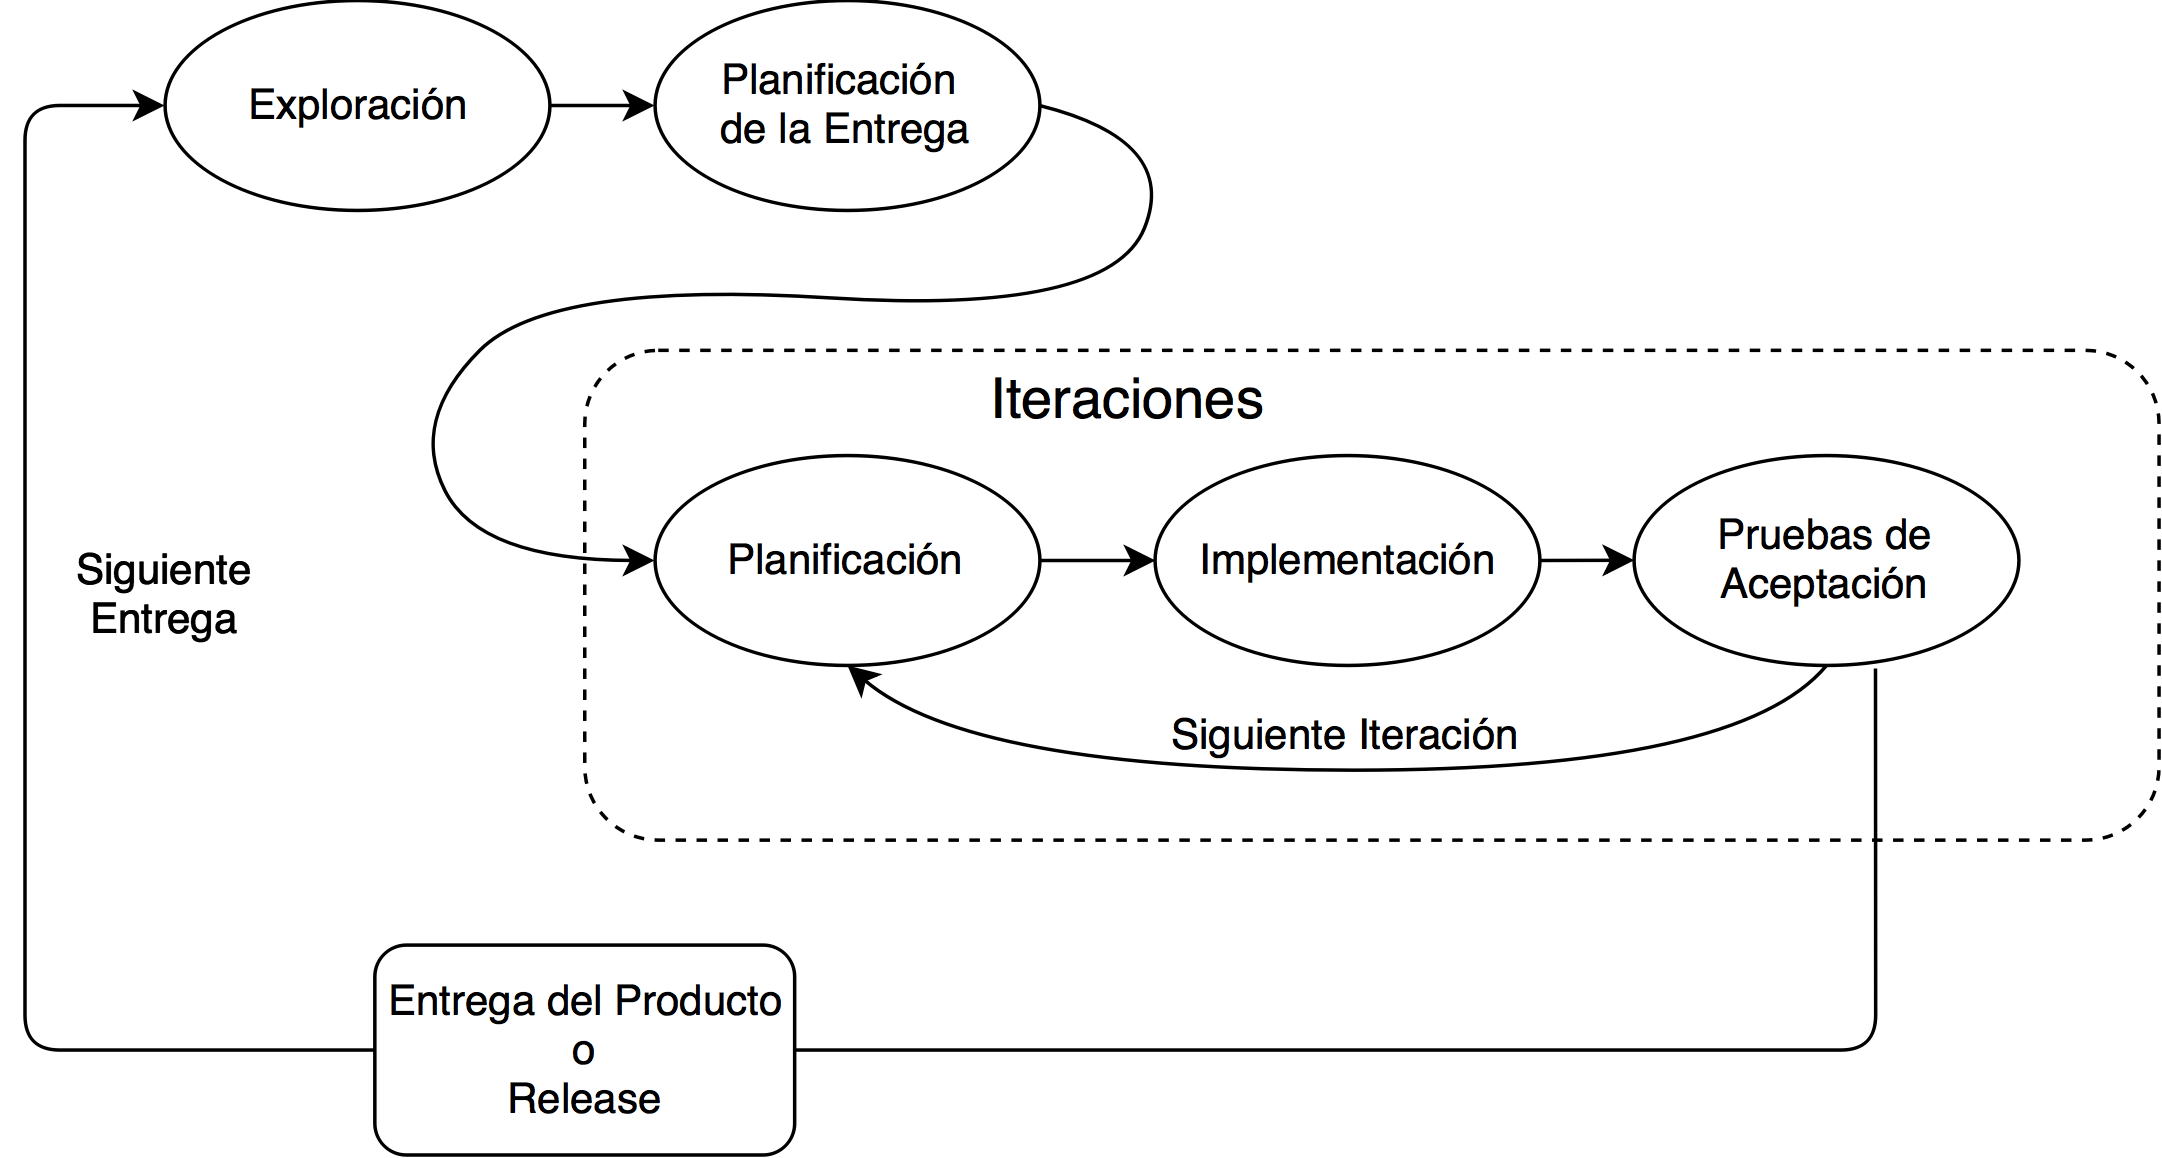
\includegraphics[width=1\textwidth]{xp_diagram}
        \end{center}
        \caption*{Fuente: Elaboración propia}
      \end{figure}

      En la figura \ref{fig:xp_diagram} se puede apreciar el proceso de desarrollo de la metodología XP, la cual se explicará a continuación.\\

        \subsection{Planning Game}
        \label{sub:planning_game}

        La fase del planning game consiste de 3 etapas: exploración, planeaci\'on y direcci\'on.\\

        Durante la fase de la \textbf{exploración} los clientes definen lo que desean que tenga el sistema y los desarrolladores estiman el tiempo necesario que necesitan para realizar esas tareas.\\

        Durante la \textbf{planeación} se negocia y se decide cuales de todas las características que los clientes quieren pueden llegar a realizarse en el tiempo dise~ado para una iteración.\\

        Después de la planeación sigue la fase de \textbf{dirección}, durante la cual se desarrolla y actualiza (cuando sea necesario) la planeación ya negociada según lo que se vaya aprendiendo a medida que avanza el desarrollo del proyecto.\\

          \subsubsection{Exploración}
          \label{subs:exploracion}
            Durante esta etapa el cliente escribe las tarjetas de historias de usuario, estas historias definen lo que el cliente quiere que el sistema haga, en otras palabras representan las características que el sistema debería tener implementado.\\

            Una vez que estas tarjetas están escritas, el equipo de desarrollo debe asignarles una estimación en términos del tiempo necesitado para el desarrollo y el riesgo para el producto que pueden llegar a tener las características detalladas en las historias del usuario.\\

            Las historias del usuario se las crea para propósitos de planeación y estimación de tiempo y esfuerzo que cada característica va a necesitar, los detalles se crean y dividen posteriormente cuando las historias están por ser implementadas en las “tareas de ingeniería”.\\
          % end exploracion

          \subsubsection{Planeación}
          \label{subs:planeacion}

            Cuando se tienen las historias del usuario junto con las estimaciones de los desarrolladores, se está listo para una “negociación de aceptación” donde un “calendario de entregas”  es negociado y donde se aceptan qué historias se van a desarrollar primero en cuanto tiempo se van a entregar resultados.\\

          % end planeacion

          \subsubsection{Dirección o Steering}
          \label{subs:steering}

          Esta fase es básicamente comprende el resto del desarrollo del producto hasta que es liberado al mercado o el proyecto es cancelado.\\

          Esta fase consiste en 4 ``movimientos'':

          \begin{description}
            \item[Iteración:] Es durante la iteración cuando se desarrolla el producto, el tiempo que se utiliza para esta fase es de generalmente de una o 2 semanas, dependiendo de la naturaleza del proyecto.

            \item[Recuperación:] Si durante el desarrollo no se completan las características a desarrollar en el tiempo establecido, es durante la recuperación que se re-negocia con el cliente si quiere cambiar la fecha de entrega del release o modificar el alcance del desarrollo (menos historias de usuario).

            \item[Nuevas Historias:] El cliente tiene el derecho de aumentar historias de usuario, las cuales se tienen que estimar y negociar si serán parte del actual desarrollo, en tal caso se tiene que renegociar las fechas de entrega.

            \item[Re-estimación:] Si durante el desarrollo el equipo considera que el plan ya no es correcto, todas las historias que faltan hacer se tienen que re-estimar y el plan se tiene que re-negociar con el cliente.
          \end{description}

        % end planning_game

          \subsection{Iteration Planning Game}
          \label{sub:iteracion}

            % \subsubsection{Iteración}
            % \label{subs:iteracion}

            La fase de Iteración en XP se lo denomina como Iteration Planning Game, esta al igual que  el release planning game consiste en las fases de: Exploración, Planning e Implementaci\'on. Steering.\\

            Hay que tomar en cuenta que la planeación de una iteración en particular es desarrollada al inicio de cada interacción, no se planifican iteraciones por adelantado.\\

            Generalmente cada 3 iteraciones se actualiza el Calendario de Entregas “committed schedule” para reflejar los logros alcanzados por el equipo de desarrollo y el estado del proyecto, también sirve para identificar posibles riesgos.\\

            \subsubsection{Exploración}
            \label{subs:exploracion}

            Durante esta fase el cliente escoge las historias de usuario que serán implementadas en la presente iteración, generalmente se escogen las que aportan más valor al producto o tienen más relevancia en la lógica de negocio del cliente, asi como tambien cualquier historia que no se acabó en una iteración anterior.\\

            Los desarrolladores dividen las historias en Tareas de Ingeniería, las cuales son más pequeñas que las historias, si se encuentra que una Tarea es casi tan grande como una historia es porque es una historia y debería ser dividida en Tareas. Una tarea puede estar relacionada a 2 o mas historias o no estar relacionada con ninguna historia. Dentro de la metodología XP es una buena práctica el escribir las tareas en las  “Index Cards”, similares a las historias, esto debido a que estas tarjetas son fáciles de manipular durante la fase de planeación.\\

            % end exploracion

            \subsubsection{Planeación}
            \label{subs:planeacion}

            Durante esta fase un desarrollador acepta la responsabilidad de implementar una Tarea de acuerdo de su experiencia personal en el área y tecnologías que se usarán en el desarrollo. El desarrollador debe estimar el tiempo necesitado para completar la tarea en un \emph{Ideal Engineering Time} Tiempo de Ingenieria Ideal, siempre hay que considerar que la tarea se deriva de la Historia de usuario que es escogido para la iteración actual, una regla de XP consiste en que no se debe realizar trabajo el cual no se va necesitar ahora, \textbf{YAGNI}\footnote{You aren't gonna need it. En espa\~nol, Tu no lo vas a necesitar \'o No vas a necesitarlo.}.\\

            La Tarea combinada con el nombre del desarrollador responsable, la estimación asignada son parte del \emph{Iteration Schedule} \'o \emph{Plan de la Iteración}, con el cual el equipo de desarrollo es capaz de determinar si la iteración está \emph{floja} o \emph{cargada}, si está \emph{floja} se pueden añadir otras historias a la iteración o si está \emph{cargada} es necesario dividir historias.\\
            Finalmente cuando la carga de trabajo de la iteración está balanceada se procede con la siguiente fase, la \emph{Implementación} de las tareas.


            % end planeacion

            \subsubsection{Implementación}
            \label{subs:implementacion}

            % dentro de la Implementación una Tarea de desarrollar.
            Dentro de lo que es el ciclo de desarrollo de software, \textbf{XP} define el siguiente procedimiento:

            \begin{itemize}
              \item Analizar lo que hay que hacer, esto envuelve lo que es analizar las Tarjetas de Ingeniería y/o las historias de usuario. %, de ser necesario se realiza una sesión CRC.
              \item Escribir Pruebas Unitarias, son bastante útiles para determinar cuando la tarea está completada.
              \item Implementar el código suficiente para lograr que las pruebas unitarias pasen exitosamente.
              \item Simplificar el código si es necesario (Refactor Mercilessly).
              \item Integrar los cambios continuamente (Continuous Integration).
            \end{itemize}
            % end implementacion

            \subsubsection{Registrar el Avance}
            \label{subs:registrar_avance}
            XP define un rol en específico que se encarga de medir el progreso, el Tracker.

            \subsubsection{Verificación}
            \label{subs:verificacion}
            Cada historia lleva asociado test funcionales, que están diseñados para verificar que los criterios de aceptación de cada historia están implementados. \\
            Si durante esta fase las pruebas fallan, la historia de usuario relacionada se marca para volver a trabajar en ella en la siguiente iteración.\\


            % end iteracion

          % end steering



        % end proceso_de_desarrollo
    % end xp


  %
  %
  % Para el presente proyecto de grado se implementará los siguientes roles:
  % Programador, Cliente, Tester, roles que serán representados por mi persona.
  % Tracker y entrenador será representado por el Tutor.
  % Consultor será representado por la docente de proyecto final


  % end metodologia_de_desarrollo

\chapter{Geolocalización} % (fold)
\label{cha:geolocalizacion}

  La Geolocalización o Georreferenciación es un término bastante nuevo, de hecho no aparece en el diccionario de la Real Academia Española, no obstante se lo puede definir como:
% \footnote{http://dle.rae.es/}

  \begin{quote}
    El posicionamiento en el que se define la localización de un objeto espacial (representado mediante un punto, vector, área, volumen) en un sistema de coordenadas y datum determinado. Este proceso es utilizado frecuentemente en los Sistemas de Información Geográfica.\cite{Georreferenciacion}
  \end{quote}

  % Para entender esta definición se necesita explicar algunos términos

  La Georreferenciación antiguamente era bastantemente usada en el ámbito científico, y se necesitaba de instrumental y personal cualificado para su manejo, pero en la actualidad la cantidad de dispositivos con capacidad para geolocalizar un objeto sobre la tierra es bastante común, de hecho todos los smartphones actuales (en general los que se consideran gama media o alta) traen integrados receptores GPS (Global Position System), y sumados a la explosión de aplicaciones  que integran mapas con localización, ya que se puede tener una base de datos con coordenadas, descripciones, etc., que individualmente no aporta mucho valor pero al obtener datos de una gran cantidad de usuarios puede llegar a ser informacion valiosa ya que sirve para tomar decisiones a nivel de negocio, pero interpretar estos datos sería muy difícil sin la ayuda de los \emph{Sistemas de Información Geográfica} o \emph{SIG}.\\

  Un SIG es una herramienta que permite integrar, analizar, mostrar, interpretar y  entender las relaciones, patrones y tendencias de la información geográficamente referenciada \cite{what_is_gis}.
  % \footnote{http://www.esri.com/what-is-gis}
  Por estas razones es que actualmente existe una explosión de estas aplicaciones, donde empresas, particulares y hasta organismos gubernamentales están haciendo uso de estas tecnologías.
  Y las posibilidades son diversas, por ejemplo, si se quisiera planificar la construcción de un colegio se podría integrar los datos del censo con un mapa, identificando los sectores con mayor porcentaje de niños y localizando los sectores más propicios para realizar la construcción del inmueble. En el caso de una catástrofe natural, el tener las rutas de evacuación geolocalizadas y disponibles en un mapa de manera eficiente,  ayudaría en la evacuación de las personas del lugar.\\

  La geolocalización es actualmente una tecnología y una herramienta usada en gran medida por una gran cantidad de aplicaciones web, añadiendo búsquedas y resultados personalizados a nivel país, ciudad, barrio y calle, resultando en una gran variedad de servicios y que actualmente es de gran ayuda en diferentes escenarios. La geolocalización ayuda a moverse por una ciudad, encontrar restaurantes, cines, transporte, etc. actualmente es una de las herramientas mas usadas y desarrolladas a nivel de industria, comercio, turismo, etc. y vale la pena estudiarla y entenderla.\\



  \section{Definiciones} % (fold)
  \label{sec:definiciones}

    En la aplicación desarrollada se requerirá trabajar con datos espaciales, y para ello es necesario entender algunos conceptos envueltos en el manejo de la información geográfica.

    \begin{description}
      \item[Coordenada:] Es una secuencia de n-números que designa la posición de un punto en un espacio n-dimensional.
      \item[Sistema de coordenadas:] Un sistema de coordenadas es  un conjunto de reglas matemáticas que especifican cómo las coordenadas son asignadas  a cada  punto.
      \item[Punto:] Es  la representación de una posición, topológicamente 0-dimensional (no tiene volumen, área, longitud o cualquier otra unidad multi-dimensional).
    \end{description}

    % \section{Coordenada} % (fold)
    % \label{sec:coordenada}
    %   Es una secuencia de n-números que designa la posición de un punto en un espacio n-dimensional. \\
    %   % one of a sequence of n-numbers designating the position of a point (4.17) in n-dimensional space
    %   % NOTA: En un
    %   % NOTE In a coordinate reference system, the numbers shall be qualified by units.

    % % subsection coordenada (end)

    % \section{Sistema de coordenadas} % (fold)
    % \label{sec:sistema_de_coordenadas}
    %   Un sistema de coordenadas es  un conjunto de reglas matemáticas que especifican cómo las coordenadas son asignadas  a cada  punto.
    %   % set of mathematical rules for specifying how coordinates (4.3) are to be assigned to each point (4.17)

    % % subsubsection sistema_de_coordenadas (end)
    % \section{Punto} % (fold)
    % \label{sec:punto}
    %   Es  la representación de una posición, topológicamente 0-dimensional (no tiene volumen, área, longitud o cualquier otra unidad multi-dimensional).
    %   % topological 0-dimensional geometric primitive (4.15), representing a position
    % % subsection punto (end)

    Estas definiciones están desarrolladas en la especificación \emph{Simple Feature Access}, la cual es mantenida por la OGC (Open Geospatial Consortium). Esta especificación define el conjunto de tipos de datos (puntos, línea, polígono, etc) y las operaciones o métodos necesarios para manejar estos datos.

    % \footnote{\url{http://www.opengeospatial.org/standards/sfa}}

  % section definiciones (end)
  \section{Sistema de Coordenadas para datos Geográficos} % (fold)
  \label{sec:sistema_de_coordenadas_para_datos_geograficos}
    Se podría pensar en un sistema de coordenadas como la forma de dar sentido a un \emph{par de coordenadas}, por ejemplo \verb|POINT(-66.1457475 -17.3937285)|, cómo se interpretan estos números?.
    Podría ser la latitud y longitud del campus de la UMSS, o algun punto en el Oceano Pacifico. Es gracias al sistema de coordenadas que se puede ubicar este punto en el Universo.\\


    Una aplicación que maneja datos geográficos tiene que trabajar con sistemas de coordenadas relacionadas con la superficie terrestre, conocidas como coordenadas espaciales o coordenadas globales, que permiten representar la tierra en \emph{3-Dimensiones} (3D), ya que esta es una Esfera, mas especificamente un esferoide oblato\footnote{Un \emph{esferoide oblato} (o elipsoide oblato) es un elipsoide de revolución obtenido por rotación de una elipse alrededor de su eje más corto.}, o en una representación de la superficie terrestre en \emph{2-Dimensiones} (2D), los sistemas de coordenadas se clasifican en: Coordenadas geocéntricas, Coordenadas Geográficas y Coordenadas Proyectadas.

    \subsection{Coordenadas geocéntricas (X,Y,Z)} % (fold)
      \label{sub:coordenadas_geocentricas}
        También conocido como \emph{Coordenadas Cartesianas 3D}, Este sistema tiene como origen el centro de la Tierra, con el \emph{eje X} y el \emph{eje Y} en el plano del ecuador. El \emph{eje X} pasa a través del meridiano de Greenwich, y el \emph{eje Z}  coincide con el eje de rotación de la Tierra. como se puede ver en la figura \ref{fig:coord_geocentric}.

        \begin{figure}[H]
          \begin{center}
            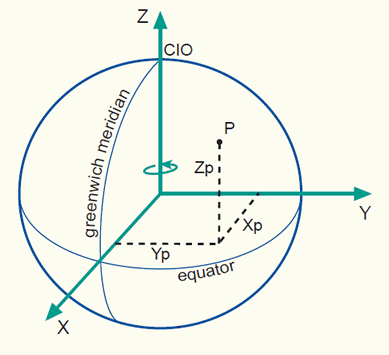
\includegraphics[width=0.7\textwidth]{coord_geocentric}
            \caption{Sistema de coordenadas Geocéntricas}
            \label{fig:coord_geocentric}
            \caption*{Fuente: \cite{coords2009} }
          \end{center}
        \end{figure}

        Este sistema de coordenadas no es muy usado en la representación de datos, pero a veces se lo requiere para análisis de algoritmos y geometría computacional.
      % subsection coordenadas_geocentricas (end)

      \subsection{Coordenadas Geográficas} % (fold)
      \label{sub:coordenadas_geograficas}
        El sistema de coordenadas Geográficas, ver figura \ref{fig:coord_geographic}, utiliza las coordenadas angulares latitud  (\emph{phi} o ${\phi}$) y longitud (\emph{lambda} o ${\lambda}$). Este sistema de coordenadas se expresa en grados, se lo puede representar con la forma \emph{grados:minutos:segundos }\verb|(17° 23' 37.4226" S, 66° 8' 44.691" W)|, o de la forma más común \emph{grados decimales} \verb|(-66.1457475 S, -17.3937285 W)|. \\

  Dentro de ese sistema de coordendas, esta el que es el más ampliamente usado y el que usan por defecto los sistemas \emph{GPS}, es el denominado ``WGS 84'' (\emph{World Geodetic System 1984}) y es el que generalmente la mayoría de las aplicaciones usan para el manejo de mapas. Es el sistema que maneja los más ampliamente conocidos ``latitud y longitud''.\\

        \begin{figure}[H]
          \begin{center}
            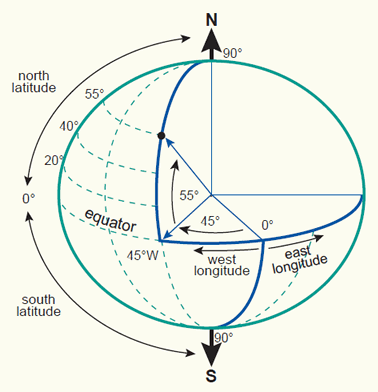
\includegraphics[width=0.7\textwidth]{coord_geographic}
            \caption{Sistema de coordenadas Geográficos}
            \label{fig:coord_geographic}
            \caption*{Fuente: \cite{coords2009} }
          \end{center}
        \end{figure}




      % subsection coordenadas_geograficas (end)

      \subsection{Coordenadas Proyectadas} % (fold)
      \label{sub:coordenadas_proyectadas}
        Un sistema de coordenadas proyectadas es una representación plana y bidimensional de la  tierra. Se basa en un sistema de coordenadas \emph{geográficas esféricas}, pero utiliza unidades de \emph{medida lineales} para las coordenadas, de forma que los cálculos de distancia y área se pueden realizar en términos de esas mismas unidades. \cite{projected}

        Un sistema de coordenadas proyectadas requiere tomar la superficie esférica de la tierra y ``aplanarla'', este procedimiento se lo realiza con la finalidad de tener un mapa representable en una hoja de papel así como en la pantalla de la computadora. Sin embargo este procedimiento introduce diversos tipos de distorsión por lo que existen diferentes clases de proyecciones que varían según la región de la Tierra que se quiere representar.

        La proyección que usan por ejemplo, \emph{Google Maps} y \emph{Open Street Maps} es la \emph{Mercator Projection}, esta proyección está diseñada para preservar los ángulos y las formas de las líneas en forma recta, pero distorsiona los tamaños y las distancias mientras más lejos se encuentran de la línea del Ecuador. Esta proyección se puede apreciar en la figura \ref{fig:mercator_proyection}. \cite{gmaps_osm}

% Google Maps usa la Proyección de Mercator para mostrar su mapa

        \begin{figure}[H]
          \begin{center}
            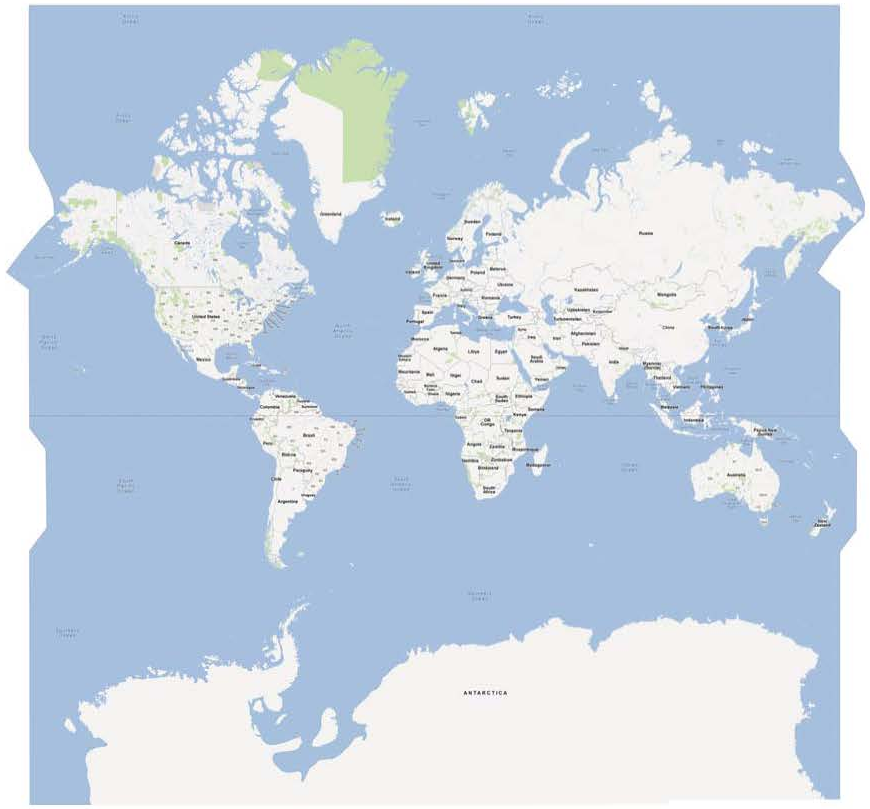
\includegraphics[width=0.6\textwidth]{mercator_proyection}
          \end{center}
          \caption{Sistema de coordenadas Proyectadas}
          \label{fig:mercator_proyection}
          \caption*{Fuente: \cite{coords2009} }
        \end{figure}

        Tal como se puede apreciar en la figura \ref{fig:mercator_proyection}, la distorsión de esta proyección se hace evidente si se observa la zona de Groenlandia ya que parecería tan grande como África o América del Sur, cosa que no es cierta, ya que Groenlandia es casi 14 veces más pequeño que África. A pesar de esta distorsión tan marcada, la \emph{Proyección de Mercator} es una de las más usadas.
         % de hecho Google Maps usa esta proyección.
      % subsection coordenadas_proyectadas (end)

  %
  %     \section{Que se usó en la Aplicación} % (fold)
  %     \label{sec:que_se_uso_en_la_aplicacion}
  %       Es importante entender las diferencias entre los distintos tipos de sistemas de coordenadas porque computacionalmente realizar operaciones sobre los sistemas de coordenadas tiene un costo.
  %       Si se usara el sistema de coordenadas geográfico (WSG84) este es el más apropiado si se necesitaría usar grandes extensiones de la superficie terrestre, que al ser una estructura elipsoidal el costo computacional para realizar las operaciones matemáticas de calcular distancias, intersecciones, etc. es más elevado. En cambio el uso de un sistema de coordenadas proyectado (Mercator Projection) tiene un costo computacional más bajo, ya que se estaría trabajando con un sistema geométrico.\\
  %
  %       % Por otro lado,
  %       También hay tomar en cuenta la base de datos, ya que será esta la que se encargará de manejar los datos espaciales. Al estar usando PostGIS, se puede ver que en su documentacion\footnote{ http://postgis.org/documentation/manual-1.5/ch04.html} que claramente exorta el uso de un sistema geometrico sobre el uso de un sistema geografico si  se va trabajar con datos que cubran una pequena area geografica. Tomando en cuenta esta recomendación y el tamaño del área de estudio (el campus de la UMSS), se procedió a implementar en la base de datos el uso de la proyección Mercator. Se va usar Mercator sobre las otras proyecciones porque aparte de las ventajas que se mencionaron con anterioridad, Google Maps usa esta proyección y ya que se usará este mapa lo más correcto es trabajar con la misma proyección.
  %
  %
  %       % Comoprojected
  %       % PostGIS maneja dos tipos de datos, geográficos y geométricos
  %
  %     % section que_se_uso_en_la_aplicacion (end)
  % % section sistema_de_coordenadas_para_datos_geograficos (end)
  % % \section{Tipo de archivos} % (fold)
  % % \label{sec:tipo_de_archivos}
  % %
  % % section tipo_de_archivos (end)
  %
  % \section{Implementación} % (fold)
  % \label{sec:Implementacion}
  %   Para manejar datos georreferenciados con tecnología JavaScript, ya que se implementó el Backend con NodeJS, se hizo uso de la librería \textbf{KnexJS} para manejar la conexión a la base de datos PostgreSQL, y BookshelfJS para las consultas SQL pero para las consultas con datos geospaciales se realizó a través de esta herramienta pero usando la forma \emph{Raw SQL}\footnote{Raw SQL se refiere a consultas en ``SQL puro'' ya que el fuerte de BookshelfJS es el manejo de las consultas en forma de objetos (ORM), lamentablemente actualmente no existe mucho soporte para manejar datos geoespaciales}.
  %
  %   \begin{center}
  %     \begin{verbatim}
  %       var raw = "SELECT " +
  %                   " ST_AsGeoJSON(geom)::json As geometry," +
  %                   " name," +
  %                   " description," +
  %                   " phone," +
  %                   " level," +
  %                   " gid As id " +
  %                 " FROM place WHERE LOWER(name)
  %                        like LOWER('%" + name + "%')";
  %     \end{verbatim}
  %   \end{center}
  %
  %   De esta forma es que se recupera de la base de datos un lugar georreferenciado, donde este tiene un nombre, una descripción, un teléfono, el nivel o piso donde se encuentra pero lo importante de esta consulta es la obtención del ``punto'' geoespacial del lugar.
  %
  %   \begin{center}
  %     \begin{verbatim}
  %       "POINT (-66.14857015827988 -17.394421906929086)"
  %     \end{verbatim}
  %   \end{center}
  %
  %   % var raw = "SELECT seq, id1 AS node, id2 AS edge, cost
  %   %            FROM pgr_dijkstra('SELECT gid AS id,
  %   %                                     source::integer,
  %   %                                     target::integer,
  %   %                                     st_length(geom) AS cost
  %   %                               FROM public.ways', targetId, sourceId, false, false);";
  %
  %
  %    Este atributo es de tipo \emph{punto} o \emph{point} el cual tiene un \emph{SRID}\footnote{ Spatial Reference System Identifier, El \emph{SRID} corresponde a un sistema de referencia espacial basado en el elipsoide concreto usado para la creación de mapas de tierra plana o de tierra redonda.\cite{msdn_srid} } \emph{3857}\footnote{La proyección Mercator usa el EPSG 3857}, el SRID  es la llave primaria de la tabla \emph{spatial\_ref\_sys} que se crea cuando se inicializa una base de datos que soporte informacion geoespacial (PostGis), esta tabla provee la información necesaria para interpretar y convertir correctamente todas las coordenadas existentes, el \emph{SRID 3857} está definida en la tabla \emph{spatial\_ref\_sys} como ``Popular Visualisation CRS / Mercator''.\\
  %
  %
  %   Obtener la coordenada es el primer paso, seguidamente se debe mostrarlo sobre un mapa, en este caso \emph{Open Street Maps}, como se puede apreciar en la figura \ref{fig:ember_leaflet}, esta interfaz está implementada usando \emph{ember-leaflet}, el cual está principalmente diseñada para ofrecer una mejor experiencia de usuario en celulares smartphones.\\
  %
  %   % \begin{center}
  %   %   \begin{verbatim}
  %   %     var maker = new google.maps.Marker({
  %   %       position: new google.maps.LatLng( lat, lng  )
  %   %       map: UMSS.map
  %   %     });
  %   %   \end{verbatim}
  %   % \end{center}
  %
  %   \begin{verbatim}
  %     {{#leaflet-map lat=lat lng=lng zoom=zoom}}
  %       {{tile-layer url="http://{s}.tile.openstreetmap.fr/hot/{z}/{x}/{y}.png" }}
  %         {{#marker-layer location=location}}
  %           <h3>{{model.name}}</h3>
  %           {{model.description}} <br>
  %           <strong>telf:</strong> {{model.phone}} <br>
  %           <strong>piso </strong>#{{model.level}}
  %       {{/marker-layer}}
  %     {{/leaflet-map}}
  %   \end{verbatim}
  %
  %   \begin{figure}[H]
  %         \begin{center}
  %           \caption{\emph{ember-leaflet} nos ayuda a desplegar un mapa y mostrar un \emph{punto} o \emph{lugar} con un \emph{marcador} y dibuja una línea de color rojo sobre el mapa.}
  %           \label{fig:ember_leaflet}
  %           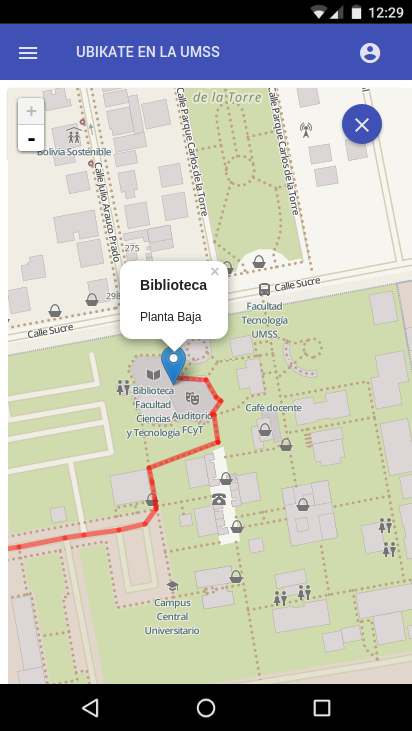
\includegraphics[width=0.5\textwidth]{ember_leaflet}
  %         \end{center}
  %         \caption*{Fuente: Elaboración propia.}
  %   \end{figure}
  %
  %

    % Pero esta coordenada  no sería  fácil de entender sin una adecuada representación sobre un mapa,


  % section Implementacion (end)
  % \section{Los datos} % (fold)
  % \label{sec:los_datos}


  %   Una vez implementada la Base de datos es necesario insertar ``los datos''
  % % section los_datos (end)


  % -------------------------------------------------------------------
  % -------------------------------------------------------------------
% -------------------------------------------------------------------

  % \section{Conclusión} % (fold)
  % \label{sec:geo_conclusion}
  %
    %
    % Los Mapas son herramientas muy útiles a la hora de desplegar información, pero realizar el mapa, crear las fórmulas matemáticas con las cuales se trabajará, determinar cómo se usarán estas fórmulas para una representación adecuada de la superficie terrestre, es una tarea muy compleja. Como programador la tarea más complicada fue determinar el tipo de mapa y el sistema de coordenadas más adecuado para el tipo proyecto que se necesita desarrollar.\\
    %
    % Los términos de longitud y latitud son en un inicio, más fácilmente comprendidos que un sistema proyectado, pero no se puede tomar a la ligera una correcta comprensión del uso de los \emph{sistemas de coordenadas} en una base de datos espacial, un mal uso de estos conceptos puede generar errores a la hora de manejar datos  espaciales o en el resultado de las operaciones sobre estos  datos, llegando a resultados no deseados y que pueden costar más tiempo y dinero en una posterior corrección.\\
    %
    %
    % Para dibujar líneas rectas sobre un mapa hay que tomar en consideración que la tierra no es plana y las líneas que en un mapa parecen líneas rectas, realmente no son rectas, ya que el planeta Tierra es un \emph{esferoide oblato} por lo que las líneas en apariencia rectas tienen la curvatura natural del planeta Tierra. En distancias largas se nota mucho mas la utilidad de usar mapas con \emph{sistemas proyectados}, pero también es cierto que para una área pequeña como es el campus de la Universidad de San Simón este problema no tiene un gran impacto pero no está demás en tomar en cuenta esta característica en el análisis de datos geoespaciales, tomando en cuenta estas caracteristacas de la Geolocalizacion se llego a la conclucion de usar
    % el sistema de \emph{coordenadas projectadas}, mas especificamente la proyección \emph{SRID 3857}.\\
    %
    %
    %
    % La geolocalización es actualmente una tecnología y una herramienta usada en gran medida por una gran cantidad de aplicaciones web, añadiendo búsquedas y resultados personalizados a nivel país, ciudad, barrio y calle, resultando en una gran variedad de servicios y que actualmente es de gran ayuda en diferentes escenarios. La geolocalización ayuda a moverse por una ciudad, encontrar restaurantes, cines, transporte, etc. actualmente es una de las herramientas mas usadas y desarrolladas a nivel de industria, comercio, turismo, etc. y vale la pena estudiarla y entenderla.\\
    %
    %
    %





% ************************************************************
    % Maps are deceivingly simple tools, and cartography a surprisingly complex discipline. While the most trouble many of us will have with a map is figuring out how to fold it, this simplicity belies great sophistication that has been developed over the years.
  % section geo_conclusion (end)


  % \begin{description}
  %   % \item[SIG] Un Sistema de Información Geográfica es una manera de visualizar como es y que está ocurriendo en algún lugar. La posibilidad de incorporar coordenadas con precisión.

  %   % A GIS is a collection of software, normally manipulated by its user through a single interface, and designed to perform a wide range of operations on geographic data.
  %   % Research  Methods in Geography
  %   % Basil Gomez and John Paul Jones III.
  %   % ISBN 978-1-4051-0710-5

  %   \item[Datum]
  %   \item[]
  %   \item[]
  % \end{description}

  % procesar
  % Se tien
  % , Sistema de Posicionamiento Global por sus siglas en espanol
% chapter geolocalizacion (end)

\section{Ruta Óptima} % (fold)
\label{cha:ruta_optima}

En general el mejor camino o el más óptimo para ir de un punto a otro es aquel que toma menos tiempo en ser recorrido, pero para definir que un camino es óptimo hay que tomar en cuenta las características de este, por ejemplo, si se va en coche hay que tomar en cuenta la dirección de las calles, los cruces, etc. si se va caminando hay que ver las características del terreno, caminos cortados, distancias, etc.\\


Encontrar la ruta óptima entre 2 puntos es un problema al cual se enfrentan las personas diariamente, por ejemplo, las empresas de transporte, de correo, etc., necesitan mejorar la eficiencia del trayecto y a la vez reducir el consumo de combustible, para mejorar la atención al cliente y a la vez reducir costos de operación. \\

Dentro el campus Universitario es generalmente prioritario optimizar el tiempo de busqueda de algun lugar o punto de interés al cual se quiera llegar, ya sea como estudiante o visitante externo.\\


Si se analiza el terreno que se va a cubrir con la aplicación, el campus ``Las Cuadras'' de la Universidad Mayor de San Simón ubicado entre las calles Oquendo, Sucre,  Belzu y M. U. López, se tiene que el camino óptimo es siempre el más corto o de menor longitud, el método de desplazamiento que se tomara en cuenta será \emph{caminando}, el terreno es llano y la única restricción es respetar las rutas peatonales.\\

% El problema de la ruta más corta es ampliamente usado por las empresas de transporte, correos, etc., que necesitan mejorar la eficiencia del trayecto y a la vez reducir el consumo de combustible, dentro del campus universitario, reducir el tiempo en el cual encontramos un aula o una oficina mejoraría en gran medida la presentación de la Universidad hacia gente externa que necesitan hacer uso o encontrar algún lugar en especifico ya que lamentablemente esta información actualmente sólo te la pueden ofrecer las personas que conocen el lugar de antemano y aun en esos casos existe la posibilidad de no encontrar el lugar que se está buscando.\\
% La resolución de este problema es la se analizará en este capítulo.

El presente problema se lo podría definir como, encontrar la ruta más corta de un punto a otro punto, donde los puntos están interconectados por una red de caminos. El problema descrito se lo puede resolver y describir como un caso específico de la teoría de grafos.



  \subsection{Grafos} % (fold)
  \label{sec:teoria_grafos}


    % \section{Definiciones} % (fold)
    % \label{sec:grafos_definiciones}
      Inicialmente es necesario aclararar algunos términos usados en la teoría de grafos.

      % El grafo que es la reprentacion

      % \begin{description}
      %   \item[Grafo] Un grafo G consiste en un conjunto  vértices V y un conjunto de aristas A, y se lo escribe como G(V,E).
      %   \item[Vertice]
      % \end{description}

      \begin{itemize}
        \item \textbf{Grafo:} Un \emph{grafo} $G$ consiste en un conjunto de vértices $V$ y un conjunto de aristas $A$, y se lo representa con $G(V,A)$.

        \item  \textbf{Vértice:} El \emph{vértice} \emph{v} es adyacente a \emph{u}, o a un vecino de \emph{u}, si y sólo si $(u,v) \in A$. Los vértices también son llamados nodos.

        \item  \textbf{Arista:}
        Cada \emph{arista} o arco es representada por un par de elementos $(u,v)$, donde los elementos $u,v \in V$, son los nodos que une la arista.

        % Para fines prácticos, no  consideraremos las aristas de la forma (u,u)

        \item \textbf{Grafo no Dirigido:}
        En un \emph{grafo no dirigido} $G$, dos vértices $u$ y $v$ se dice que están conectados si hay un camino en $G$ de $u$ a $v$ (y cómo $G$ no es dirigido, también hay un camino de $v$ a $u$). Un grafo  se denomina completo si para todos los pares $u,v \in V$ existe una arista $(u,v) \in A$.

        % En un \emph{grafo no dirigido}, dado una arista $(u,v)$, $v$ es adyacente de $u$, y simétricamente \emph{u} es adyacente de \emph{v} y si el par de vértices que representan la arista no tiene orden, por lo tanto la arista $(u,v)$ y $(v,u)$ representa la misma arista.

        \item \textbf{Grafo Dirigido:} En cambio en un \emph{grafo dirigido} las aristas $(u,v)$ y $(v,u)$ representan dos diferentes aristas. También se puede anotar un tercer componente, llamado peso o costo, en ese caso estaríamos hablando de un \emph{grafo ponderado}.

        % Un camino en un grafo es una secuencia de nodos $v_{1}$, $v_{2}$, \ldots{}, $v_n$ tal que $(v_{1}, v_{2}), (v_{2}, v_{3}), \ldots{}, (v_{n-1}, v_n)$ son aristas.
        %
      \end{itemize}



    % \end{description}
    % subsection grafos_definiciones (end)
    % \subsection{Representacion de un Grafo} % (fold)
    % \label{sec:representacion_de_un_grafo}
      Existen diversas formas de representar un grafo sea dirigido o no-dirigido, pero entre las mas usadas están la matriz de adyacencias y la lista de adyacencias.

      \subsection{Matriz de adyacencias de un Grafo} % (fold)
      \label{sub:matriz_de_adyacencias_de_un_grafo}
        Sea $G = (V,A)$ un grafo de \emph{n} vértices. La matriz de adyacencias $M$  para $G$ es una matriz $M_{nxn}$ de valores booleanos, donde $M(i,j)$ es verdad si y sólo si existe un arco desde el nodo \emph{i} al nodo \emph{j}.

        \begin{displaymath}
          M(i,j) = \left\{
          \begin{array}{ l l }
            1, & \textrm{si existe la arista } (i,j) \\
            0, & \textrm{en caso contrario}
          \end{array} \right.
        \end{displaymath}


        Las filas y las columnas de la matriz representan los nodos del grafo.
        Cuando el grafo es no-dirigido la matriz de adyacencias es simétrica, como se puede ver en el grafo de la figura \ref{fig:grafo_ponderado} y su correspondiente matriz de adyacencias.
        % El cuadro \ref{tab:matriz} representa la matriz de adyacencias de la figura \ref{fig:grafo_ponderado} representa
        % La matriz de adyacencias, que se puede observar a continuacion, es la  misma matriz de la relación $A$ de $V$ en $V$ porque indica cuales vertices están relacionados o unidos por una arista.


        % \begin{tikzpicture}[->,>=stealth',shorten >=1pt,auto,node distance=3cm,
        %         main node/.style={circle,draw,font=\sffamily\Large\bfseries}]
% !ht
        \begin{figure}[H]
          \begin{center}

            \begin{tikzpicture}[->,>=stealth',shorten>=1pt,auto,node distance=3cm,main node/.style={circle,draw,font=\sffamily\Large\bfseries}]

              \node[main node] (1) {a};
              \node[main node] (2) [below right  of=1] {b};
              \node[main node] (3) [above right of=2] {c};
              \node[main node] (4) [below left of=2] {d};
              \node[main node] (5) [right of=2] {e};
              % \node[main node] (6) [right of=5] {f};
              % \node[main node] (7) [above right of=6] {g};
              % \node[main node] (4) [below right of=1] {d};

              \path[every node/.style={font=\sffamily\small}]
                (1) edge node [auto] {3} (2)
                    edge node[left] {5} (4)
                (2) edge node[left] {8} (3)
                    edge node[right] {4} (4)
                    edge node[auto] {3} (5)
                (3) edge node[left] {7} (5)
                (4) edge node[below] {14} (5);

            \end{tikzpicture}

            \caption{Grafo ponderado no-dirigido}
            \label{fig:grafo_ponderado}
            \caption*{Fuente: Elaboración propia}

          \end{center}
        \end{figure}

        % La matriz de adyacencias, que se puede observar a continuacion, es la  misma matriz de la relación $A$ de $V$ en $V$ porque indica cuales vertices están relacionados o unidos por una arista.


        \begin{table}[H]
          % \label{tab:matriz}
          \begin{center}
            \begin{displaymath}
              M(i,j) =
              \bordermatrix{ ~ & a & b & c & d & e \cr
                             a & 0 & 3 & 0 & 5 & 0 \cr
                             b & 3 & 0 & 8 & 4 & 3 \cr
                             c & 0 & 8 & 0 & 0 & 7 \cr
                             d & 5 & 4 & 0 & 0 & 14\cr
                             e & 0 & 3 & 7 & 14& 0  }
            \end{displaymath}
            \caption*{Matriz de adyacencias del grafo de la figura  \ref{fig:grafo_ponderado}}
          \end{center}
        \end{table}


      % subsubsection matriz_de_adyacencias_de_un_grafo (end)

    % subsection representacion_de_un_grafo (end)
    \subsection{El Problema de la ruta mas corta} % (fold)
    \label{sec:ruta_mas_corta}
      Dados los vértices $v_{i}$ y $v_{j}$ de un grafo $G = (V,A)$ se llama trayectoria mínima o camino minimo  de \(v_i\) a \(v_j\) al numero de aristas del camino de longitud mínima que va desde $v_i$ a $v_j$ y se representa por $d(v_i, v_j)$.

      Cuando en el grafo no exista un camino de $v_i$ a $v_j$ se dice que el camino minimo es $d(v_i, v_j) = \infty$ \\

      Para determinar el camino mínimo que va desde un único vértice a cualquier otro vértice se puede usar el algoritmo de Dijkstra.



      \subsubsection{Algoritmo de Dijkstra} % (fold)
      \label{sub:algoritmo_de_dijkstra}
      El algoritmo de  Dijkstra fue descrito en 1959 por \emph{Edsger Dijkstra}, y permite encontrar la trayectoria más corta entre dos nodos específicos, cuando los valores de los arcos son todos positivos\\

      El algoritmo asigna un etiqueta a cada nodo en el grafo. Esta etiqueta es la distancia que hay desde el nodo \emph{s} escogido como origen a lo largo de la trayectoria más corta encontrada, hasta el nodo que se está etiquetando.\\

      La etiqueta de cada nodo puede estar en 2 estados:

      \begin{itemize}
        \item[\textbf{a.}] Puede ser permanente; en este caso la distancia encontrada es a lo largo de la trayectoria, la más corta de todas las encontradas.
        \item[\textbf{b.}] Puede ser temporal; cuando hay incertidumbre de que la trayectoria encontrada sea la más corta de todas.
      \end{itemize}

      A medida que el método trabaja se cambian gradualmente las etiquetas temporales por etiquetas permanentes. Al comienzo se tiene un conjunto de nodos con etiquetas temporales y el objetivo es hacer que esas etiquetas disminuyan, encontrando trayectorias a esos nodos usando trayectorias a nodos etiquetados permanentemente. Cuando esto se ha logrado, se selecciona el nodo con la etiqueta temporal más pequeña y esta etiqueta se convierte en permanente. El proceso se repite hasta que al nodo terminal \emph{t} se le haya asignado una etiqueta permanente, pero esto puede ocurrir eventualmente, ya que cada vez que el algoritmo es usado, una de las etiquetas es omitida y así el número de nodos con etiquetas temporales decrece a cero. \cite{teoria_grafos} \\


      % subsection algoritmo_de_dijkstra (end)
    % subsection ruta_mas_corta (end)
  % section teoria_grafos (end)


% ********************************************************************
% ********************************************************************
% ********************************************************************

  % \subsection{Conclusi\'on} % (fold)
  % \label{sub:ruta_conclusion}


    % ********************************************************************
    % ********************************************************************
% ********************************************************************

  % section ruta_conclusion (end)
% chapter ruta_optima (end)


  % Algoritmos de busqueda de caminos - ruta corta

  % Como determino que tipo de grafo tengo


  % % \section{La Red} % (fold)
  % % \label{sec:la_red}

  % % % section la_red (end)

  % \section{Algoritmo} % (fold)
  % \label{sec:algoritmo}

  % % section algoritmo (end)

  % \section{Algoritmo de Dijkstra} % (fold)
  % \label{sec:algoritmo_de_dijkstra}

  % % section algoritmo_de_dijkstra (end)

  % % Por lo tanto se implementó un grafo no dirigido (sin dirección), el cual se analizará en este capítulo.


  % Un problema de este tipo es represetable como un proble de teoria de grafos.


  % Cuando se tiene que encontrar un camino o ruta optima entre 2 puntos, se tienen que tomar en cuenta varios puntos


  % El problema de encontrar una ruta optima entre 2 puntos se lo puede resolver/representar como problema de grafos


  % Caminos mínimos en grafos

  % Solución voraz: Algoritmo de Dijkstra

  % para grafos dirigidos (la extensión a no dirigidos es inmediata)
  % genera uno a uno los caminos de un nodo v al resto por orden creciente de longitud
  % usa un conjunto de vértices donde, a cada paso, se guardan los nodos para los que ya se sabe el camino mínimo
  % devuelve un vector indexado por vértices: en cada posición w se guarda el coste del camino mínimo que conecta v con w
  % cada vez que se incorpora un nodo a la solución se comprueba si los caminos todavía no definitivos se pueden acortar pasando por él
  % se supone que el camino mínimo de un nodo a sí mismo tiene coste nulo
  % un valor en la posición w del vector indica que no hay ningún camino desde v a w
  % E.W. Dijkstra:
  % “A note on two problems in connexion with graphs”,
  % Numerical Mathematica, 1, pp. 269-271, 1959.


  \chapter{Caso Estudio: Campus Universitario}
\label{chap:Caso Estudio: Campus Universitario}


En el presente proyecto se implementó una aplicación web móvil, como ya se explico, este tipo de aplicaciones son básicamente páginas web, con amplia funcionalidad e implementadas específicamente para su uso en dispositivos móviles, tablets o smartphones, para lo cual se investigó las tecnologías, arquitecturas y los frameworks de desarrollo que actualmente usan este tipo de aplicaciones, una de los concepto que se estudió fue de las \emph{aplicaciones de página única}, concepto que se empezó a discutir a principios de 2003, y se puso de moda con la aparición de frameworks JavaScript que agilizan y facilitan en gran medida la implementación de aplicaciones web, tales como \emph{AngularJS}, \emph{BackboneJS} y en el 2010 \emph{EmberJS}. \\

Es necesario reconocer las diferentes partes con la que cuenta una aplicación web móvil como una aplicación de página única diseñada para dispositivos móviles, es necesario implementar un REST API que se encargue de hacer las consultas a la base de datos y que el cliente pueda consumir la información obtenida de la base de datos así como también el camino inverso, la base de datos necesita manejar informacion geoespacial y el cliente necesita que la aplicación sea optimizada para su uso en dispositivos móviles. Tomando en cuenta estos requerimientos se puede separar el desarrollo del proyecto en los siguientes apartados. \\



\section{Generar el mapa con información geográfica}
\label{sec:generar_mapa_rutas}

Para poder responder al problema de encontrar una ruta óptima entre 2 puntos dentro del campus universitario, se necesita de un mapa que contenga todas las rutas que existen dentro del campus.\\

 %
 %
 % \section{Campus Universitario}
 % \label{sec:ruta_corta_umss}

 En primer lugar fue necesario obtener un grafo ponderado no-dirigido que represente un mapa de los caminos que existen dentro del campus Universitario.\\

 Para obtener este mapa se procedió a caminar a través del campus de la UMSS con un GPS Garmin Nuvi 1300, el cual es un dispositivo GPS básico pero cumple con la función de guardar información geográfica, los archivos generados tienen extensión \emph{gpx}, que básicamente es un fichero XML estándar usado para compartir datos entre GPS's, se recorrieron los principales caminos que existen e interconectan las distintas facultades y oficinas dentro del campus universitario. Una vez realizado este recorrido, se procedió a extraer la información del dispositivo GPS, se utilizó el archivo \emph{current.gpx} para exportar la información  a un archivo \emph{shapefile}, para esta tarea se utilizó QGis, con el cual se acabó editando las rutas recogidas por el GPS.\\

% \footnote{Un shapefile es un archivo de formato sencillo y no topológico que se utiliza para almacenar la ubicación geométrica y la información de atributos de las entidades geográficas.\cite{what_is_shapefile} }

 Este paso fue necesario porque el mapa extraído del GPS es una línea única, pero para que nos sirva para el objetivo de buscar una ruta óptima, es necesario que esta línea sea dividida o separada en muchas líneas, las cuales son las aristas y los extremos de las líneas serán los nodos o vértices del grafo.\\

 Implementando el algoritmo de \emph{Dijkstra} en el grafo resultante es lo que nos permitir\'a encontrar la ruta más corta dentro del campus Universitario, al tener una gran cantidad de información resultante de la obtención de datos mediante un dispositivo GPS se hace imprescindible usar una base de datos que nos ayude con esta tarea, para lo cual se usó la base de datos PostgreSQL añadiendolo PostGIS y pgRouting, herramientas ampliamente utilizadas en el manejo de datos geo-espaciales.\\

  % el grafo representa el mapa de caminos  pueda ser usado en una base de datos  “ruteable”, esto significa que el mapa de una sola línea hay que separarlo o dividirlo en muchas líneas.\\


 Técnicamente esta línea única es representada como un \emph{POLYLINE} el cual consiste en una o más partes. Una parte es una secuencia conectada de dos o más puntos. Las partes pueden o no estar conectadas entre sí. Las partes pueden o no intersectarse entre sí, para transformar este POLYLINE necesitamos separar todas sus partes y convertirlas en objetos \emph{LINESTRING} únicos, y a este conjunto de LINESTRINGs es el que se va a usar en la base de datos como mapa de ``rutas''.\cite{esri_shapefile}\\

 \begin{figure}[H]
   \begin{center}
     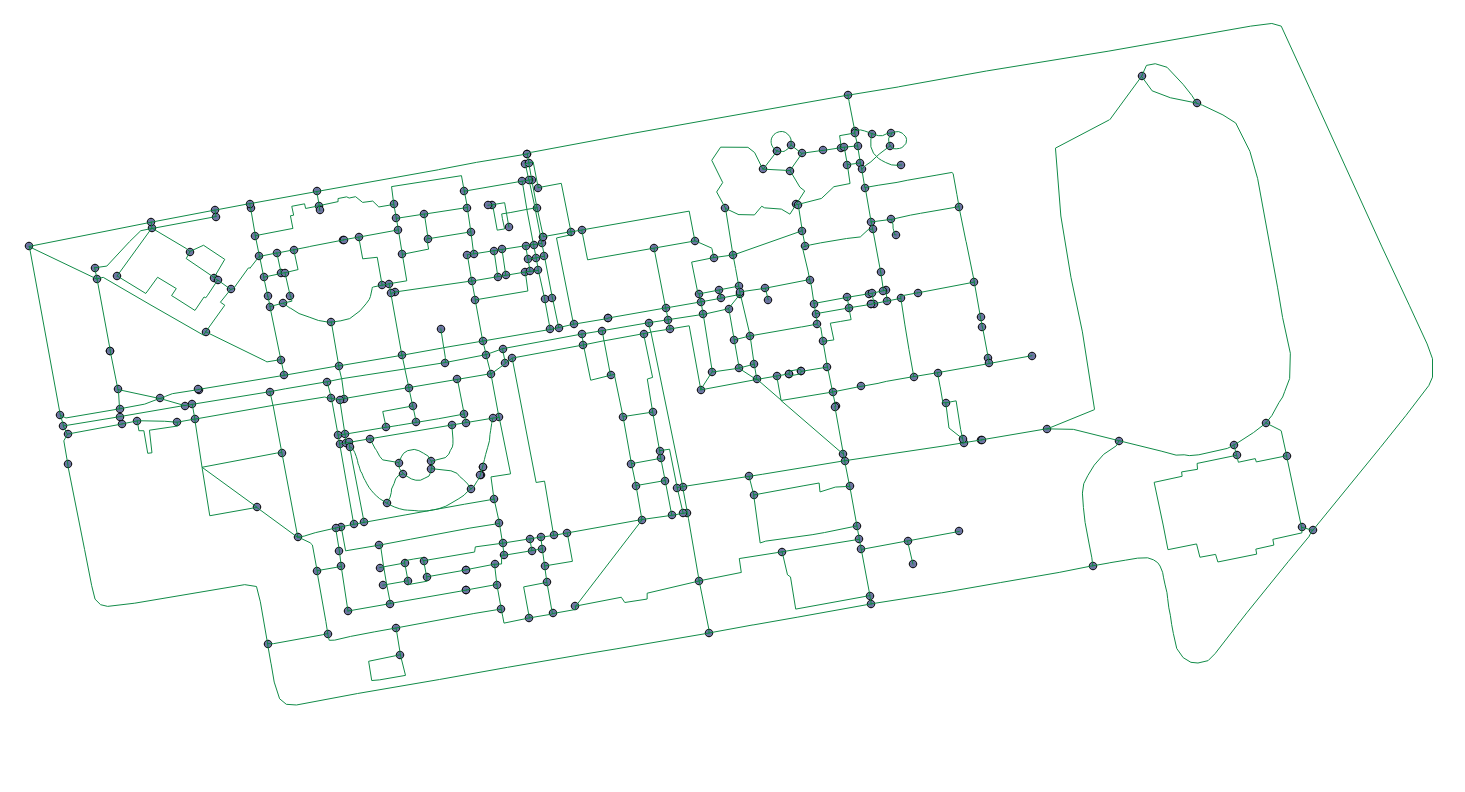
\includegraphics[width=1\textwidth]{shapefile_umss_v1}
     \caption{Shapefile del campus Universitario.}
     \label{fig:shapefile_umss_v1}
     \caption*{Fuente: Elaboración propia}
   \end{center}
 \end{figure}

 En la figura \ref{fig:shapefile_umss_v1} se puede apreciar el shapefile resultante de la división del POLYLINE original, las líneas que conforman el mapa de las rutas del campus Universitario, donde cada línea es una arista y los puntos son los nodos del grafo no-dirigido, que será usado para la resolución del problema de la ruta más corta en el presente proyecto de grado.\\

 Para una mejor apreciación del grafo que consta de 1164 aristas y 1003 vértices, se lo puede ver en combinación o proyectada en un mapa de rutas del campus de la Universidad Mayor de San Simón ubicado entre las calles Oquendo, Sucre y  Belzu de la ciudad de Cochabamba - Bolivia, se puede referir a la siguiente figura \ref{fig:shapefile_umss_v2}.

 \begin{figure}[H]
   \begin{center}
     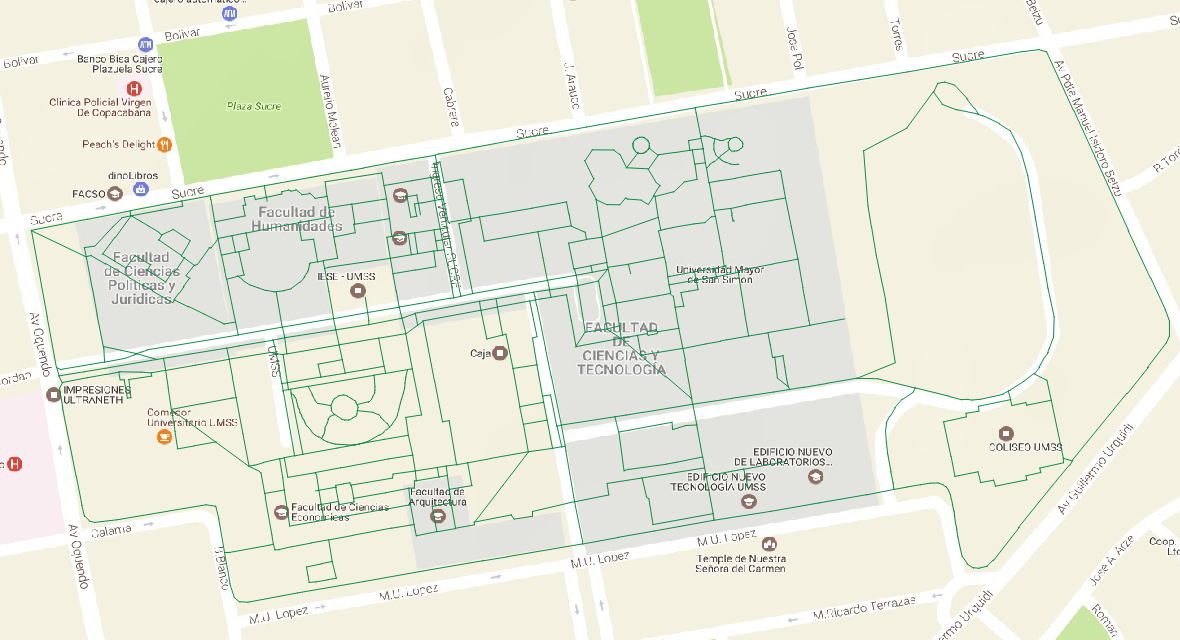
\includegraphics[width=1\textwidth]{shapefile_umss_v2}
     \caption{Shapefile sobre el campus Universitario de la UMSS.}
     \label{fig:shapefile_umss_v2}
     \caption*{Fuente: Elaboración propia}
   \end{center}
 \end{figure}


 \subsection{Facultad de Derecho}
 \label{sub:facultad_derecho}

 La facultad de Derecho cuenta con alrededor de 178 vértices y 88 aristas, está ubicada al nor-oeste del Campus Universitario, en la esquina de la calle Oquendo y Sucre, dentro del campus colinda con la facultad de Humanidades hacia el Nor-Este y hacia el Sur-Oeste está la facultad de Economía.

 \begin{figure}[H]
   \begin{center}
     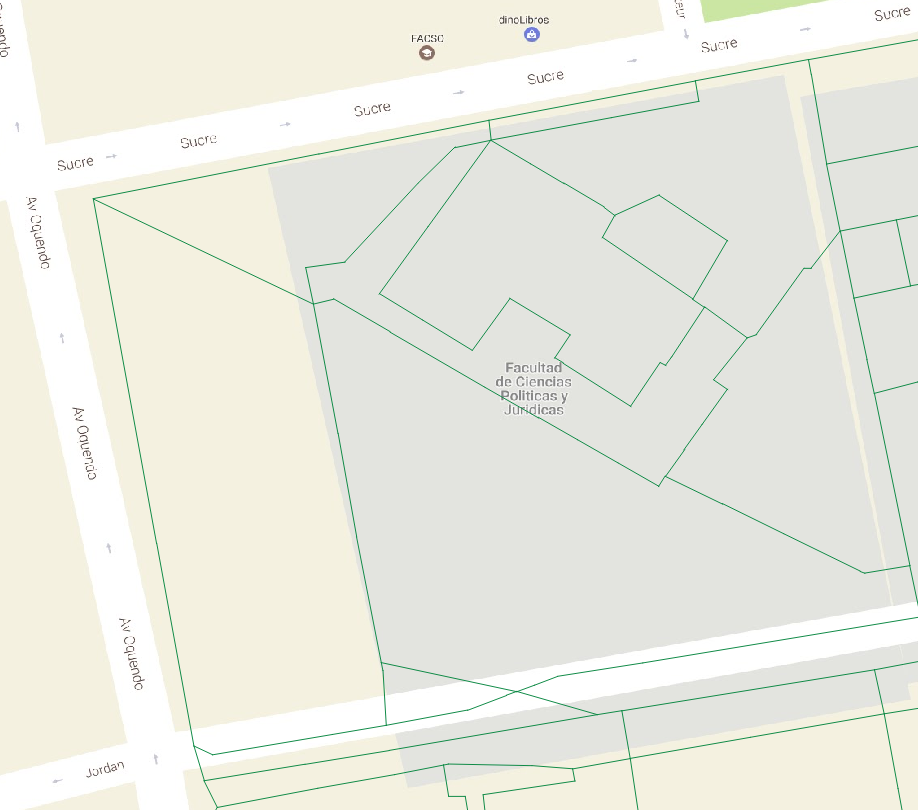
\includegraphics[width=0.75\textwidth]{fac_derecho}
     \caption{Facultad de Derecho - UMSS}
     \label{fig:fac_derecho}
     \caption*{Fuente: Elaboración propia}
   \end{center}
 \end{figure}

 En la figura \ref{fig:fac_derecho} se puede observar en la línea verde los caminos o rutas dentro de la facultad de derecho de la UMSS, proyectada sobre el mapa de Google Maps, para lograr esta representación se utilizó QGIS ya que la información geográfica de la ruta está contenida en un archivo shapefile y el mapa se lo obtiene usando el API de Google Maps gracias al plugin de QGIS, \emph{QuickMapServices}.

 % \footnote{http://nextgis.com/blog/quickmapservices/}.


\subsection{Facultad de Economía}
\label{sub:facultad_economia}

La facultad de Economía está compuesta de XX aristas y XXX vértices, está ubicada en el sector Sur-Oeste del campus Universitario, colinda con las calles Oquendo y M. U. López, dentro del campus al Nor-Este se encuentra la facultad de Arquitectura y al Nor-Oeste la facultad de Derecho, tal como se puede apreciar en la figura \ref{fig:fac_economia}.

\begin{figure}[H]
 \begin{center}
   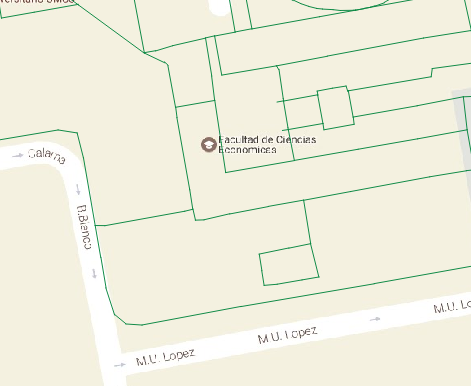
\includegraphics[width=0.75\textwidth]{fac_economia}
   \caption{Facultad de Economia - UMSS}
   \label{fig:fac_economia}
   \caption*{Fuente: Elaboración propia}
 \end{center}
\end{figure}



\subsection{Facultad de Humanidades}
\label{sub:facultad_humanidades}

La facultad de Humanidades está compuesta por XX aristas y XXX vértices, colinda con la calle Sucre hacia el Nor-Oeste, dentro del campus Universitario se encuentra la facultad de Tecnología hacia el Nor-Este, hacia el Sur-Oeste está la Facultad de Derecho y al Sur-Este se encuentra la Facultad de Arquitectura, en la figura \ref{fig:fac_humanidades} se puede apreciar la facultad de Humanidades dentro del campus Universitario sobrepuesto con el mapa de rutas identificado por la línea verde.

\begin{figure}[H]
 \begin{center}
   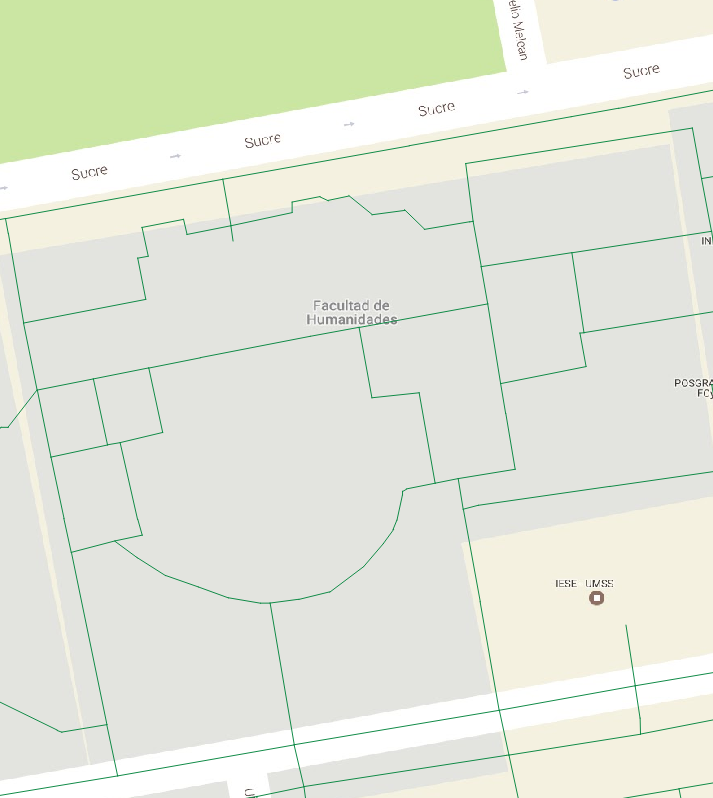
\includegraphics[width=0.75\textwidth]{fac_humanidades}
   \caption{Facultad de Humanidades - UMSS}
   \label{fig:fac_humanidades}
   \caption*{Fuente: Elaboración propia}
 \end{center}
\end{figure}


\subsection{Facultad de Tecnología}
\label{sub:facultad_tecnologia}

La facultad de Tecnología se encuentra en el extremo Nor-Este dentro del campus Universitario y cuenta con XX aristas y XXX vértices, la facultad de tecnología colinda hacia el Nor-Oeste con la calle Sucre, y hacia el Este con la calle Belzu, dentro del campus Universitario colinda con las facultades de Arquitectura y Humanidades que se encuentran hacia el Sur-Este y Sur-Oeste correspondientemente, en la siguiente figura \ref{fig:fac_tecno} se puede apreciar el mapa de rutas de la facultad de Tecnología.

\begin{figure}[H]
 \begin{center}
   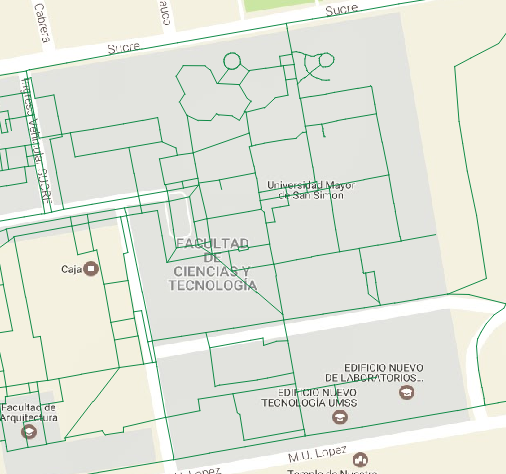
\includegraphics[width=0.75\textwidth]{fac_tecno}
   \caption{Facultad de Tecnologia - UMSS}
   \label{fig:fac_tecno}
   \caption*{Fuente: Elaboración propia}
 \end{center}
\end{figure}

\subsection{Facultad de Arquitectura}
\label{sub:facultad_arquitectura}

El grafo correspondiente a la facultad de Arquitectura cuenta con XX aristas y XXX vértices, la facultad colinda con la calle M. U. Lopez, dentro de los predios del campus Universitario se halla entre las facultades de Economía hacia el Sur-Este y con la facultad de Tecnología hacia el Nor-Oeste, el grafo se puede apreciar en la siguiente figura \ref{fig:fac_arqui}.

\begin{figure}[H]
 \begin{center}
   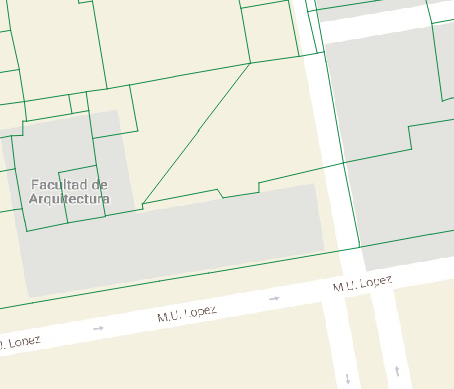
\includegraphics[width=0.75\textwidth]{fac_arqui}
   \caption{Facultad de Arquitectura - UMSS}
   \label{fig:fac_arqui}
   \caption*{Fuente: Elaboración propia}
 \end{center}
\end{figure}






\section{Backend}
\label{sec:Backend}

El backend de la aplicación comprende el manejo de la información y cómo es procesada para su consumo por parte del frontend y almacenamiento en la base de datos, por lo tanto se pueden observar dentro del backend, 2 secciones claramente diferenciadas: el servidor web y la base de datos.\\




\subsection{Servidor Web}
\label{sub:servidor_web}

Un servidor web se puede referir a 2 cosas, la primera es la máquina en la cual se instalará y alojara toda la lógica de negocio que requiere la aplicación, la segunda se refiere a la capacidad de poder recibir y dar información al cliente del servidor, el segundo caso es también conocido como un \emph{servicio web} el cual será discutido en esta sección.\\

El servidor web es el encargado de enviar la página HTML la primera vez que el cliente hace un request al servidor, una vez que la página está cargada el servidor solo se encarga de enviar y recibir información de la base de datos al cliente.\\

El servidor web será construido con \emph{Express JS}, para lo cual primeramente se necesita instalar \emph{Node JS}, \emph{Express JS} cuenta con una herramienta para la consola, \emph{express-generator}, entonces solo es necesario crear un projecto Express y empezar a implementar la lógica de negocio.\\

El servidor se va a encargar de hablar con la base de datos y también necesita ofrecer una interfaz por la cual pueda recibir datos y entregar datos, en pocas palabras un \emph{API}, implementar un \emph{API} con \emph{Express} es bastante sencillo, para trabajar con la base de datos se instaló una librería \emph{BookshelfJS} para poder escribir las consultas y trabajar con la base de datos como si se tratara de objetos, este patrón se denomina \emph{ORM} o \emph{Object-Relational-Model}, básicamente mapea las tablas y las relaciones existentes como objetos dentro del paradigma \emph{OOP} y el framework se encarga de traducirlo a lenguaje \emph{SQL} que es el lenguaje que entienden las bases de datos, \emph{BookshelfJS} también permite escribir las consultas en lenguaje \emph{SQL} si fuera necesario, como en el presente caso ya que al  trabajar con una herramienta específica, \emph{pgRouting}, las consultas son personalizadas.\\

% \begin{minted}{js}
 \begin{center}
   \begin{verbatim}
     var getPlace = (req, res) => {
       var id = req.params.id;
       var raw = "SELECT " +
                 " ST_AsGeoJSON(geom)::json As geometry," +
                 " name," +
                 " description," +
                 " phone," +
                 " level," +
                 " gid As id " +
                 " FROM place WHERE gid = " + id;
       Bookshelf.knex.raw(raw)
         .then((data) => {
           res.json(data.rows[0]);
       })
         .catch((error) => {
           console.log(error);
           res.send("Error");
       });
     };
   \end{verbatim}
 \end{center}
 %  \end{minted}

Como en la anterior consulta, se requiere obtener la información de un lugar, por lo tanto se necesita  usar la forma \emph{Raw SQL} o consultas en ``SQL puro'' ya que el fuerte de \emph{BookshelfJS} es el manejo de las consultas en forma de objetos (ORM), lamentablemente actualmente no existe mucho soporte para manejar datos geoespaciales por parte de frameworks ORM.\\

% De esta forma se obtiene de la base de datos la infor  donde este
Una vez que se obtiene la información del lugar; nombre, descripcion, telefono, el nivel o piso, pero lo importante de esta consulta es la obtención del ``punto'' geoespacial del lugar. Estos datos son importantes para implementar la lógica de negocio.\\


\begin{center}
 \begin{verbatim}
   "POINT (-66.14857015827988 -17.394421906929086)"
 \end{verbatim}
\end{center}

% var raw = "SELECT seq, id1 AS node, id2 AS edge, cost
%            FROM pgr_dijkstra('SELECT gid AS id,
%                                     source::integer,
%                                     target::integer,
%                                     st_length(geom) AS cost
%                               FROM public.ways', targetId, sourceId, false, false);";


Este atributo es de tipo \emph{punto} o \emph{point} el cual tiene un \emph{SRID} o \emph{Spatial Reference System Identifier}, el \emph{SRID} corresponde a un sistema de referencia espacial basado en el elipsoide concreto usado para la creación de mapas de tierra plana o de tierra redonda.\cite{msdn_srid}\\

El \emph{SRID 3857} también conocido como \emph{EPSG 3857} es la implementada en la \emph{Proyección de Mercator}, el SRID  es la llave primaria de la tabla \emph{spatial\_ref\_sys} que se crea cuando se inicializa \emph{PostGis} en una base de datos para que esta soporte informacion geoespacial, esta tabla provee la información necesaria para interpretar y convertir correctamente todas las coordenadas existentes, el \emph{SRID 3857} está definida en la tabla \emph{spatial\_ref\_sys} como ``Popular Visualisation CRS / Mercator''.\\

En resumen el servidor web será el encargado de recibir información y devolver una respuesta de acuerdo a los datos que recupere de la base de datos, para tal efecto se utilizan las direcciones URL, las cuales de acuerdo al protocolo HTTP se pueden definir de acuerdo a la acción que el servidor necesita procesar, para lograr esta comunicación es necesario definir nuestro API.\\


\subsubsection{Implementación del REST API}
\label{subs:Implementacion del REST API}



El servidor necesita reconocer las peticiones que le llegan del cliente, para lo cual es necesario ``mapear'' un URI a una acción específica, las cuales ya están preparadas para comunicarse con la base de datos, no hay restricción en la declaración de las URIs pero para una mejor comprensión del API que se está desarrollando es necesario seguir convenciones que aseguran que cualquier desarrollador pueda comprender el API presentado y pueda ser fácilmente consumido por cualquier aplicación que requiera acceder a la información que disponible, un API REST es el que cumple con estas características.
En primer lugar es necesario crear las URIs que serán ``entendidas'' por el servidor, esto se logra declarando en el servicio creado con \emph{Express.JS}, tal como se puede apreciar en el siguiente bloque de código, cada URI se lo relaciona a un modelo en específico de acuerdo a la acción que se requiere, tal como se puede observar en el cuadro \ref{tab:rest} las URIs declaradas en el API cumplen con tal característica.\\


% \begin{minted}{js}[label=express_api,caption=Declarando API REST con ExpressJS]
\begin{center}
  \begin{lstlisting}[label=express_api,caption=Declarando API REST con ExpressJS]
        const router = express.Router();
        router.get('/', places.getAll);
        router.get('/:id', places.getPlace);
        router.post('/', places.newPlace);
        router.put('/:id', places.editPlace);
        router.delete('/:id', places.deletePlace);

        app.use('/api/v1/places', router);
  \end{lstlisting}
\end{center}
% \end{minted}

% En el código

  %
  % Para lograr todo este comportamiento  es necesario declarar, en el archivo
  % que controla las rutas dentro de la aplicación, \textbf{routes}, que el
  % recurso \textbf{user} es \emph{restful}, tal como se muestra en la figura \ref{fig:rest}\\

  % \begin{figure}[!hbp]
  %   \begin{center}
  %     \caption[REST - routes.rb]{config/routes.rb}
  %     \label{fig:rest}
  %     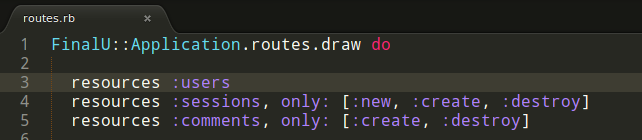
\includegraphics[width=1\textwidth]{rest}
  %     \caption*{Fuente: }
  %   \end{center}
  % \end{figure}

  El cuadro \ref{tab:rest} muestra como se puede leer las peticiones al API de \textbf{places}, las acciones mostradas son las que se pueden encontrar en un API REST pero no es necesario declararlas todas para considerar a que un API es restful.\\


  \begin{table}[!hbp]
    \begin{center}

      \begin{tabularx}{0.75\textwidth}{ l l l  X }
        \toprule
        \multicolumn{1}{c}{\textbf{HTTP}} &
        \multicolumn{1}{c}{\textbf{URI}}  &
        % \multicolumn{1}{c}{\textbf{C}}  &
        \multicolumn{1}{c}{\textbf{ACCI\'ON}} &
        \multicolumn{1}{c}{\textbf{USADO PARA}}  \\
        \multicolumn{1}{c}{\textbf{request}} & & & \\

        \midrule
        GET     &  /places    &  index    & devuelve una lista con todos los lugares\\
        POST    &  /places    &  create   & inserta un nuevo lugar en la bd\\
        GET     &  /places/1  &  show     & muestra el lugar con identificador \emph{1}\\
        PUT     &  /places/1  &  update   & actualiza los datos de un lugar específico\\
        DELETE  &  /places/1  &  delete   & elimina el lugar con id = 1 de la bd\\
        \bottomrule
      \end{tabularx}

      \caption[recursos REST]{REST URIs para los lugares}
      \label{tab:rest}

      \caption*{Fuente: Elaboración propia}
    \end{center}
  \end{table}

  % Tal como se ve en el cuadro \ref{tab:rest}, Rails maneja los request HTTP de acuerdo con
  % el tipo de llamada que se realice, este trabajo lo realiza el \textbf{router},
  % que reconoce las URLs y los despacha a una \textbf{acción} del controlador,
  % todo este proceso ya está implementado en el núcleo de Rails por lo tanto  es automático y el programador
  % no necesita más configuración que la mostrada en la figura \ref{fig:rest},
  % obedeciendo al principio de \emph{Convención sobre configuración}\\

  % % no son más que métodos dentro del \emph{user\_controller.rb}
  % el cual
  % es parte del controlador de la arquitectura MVC.\\

  % The Rails router recognizes URLs and dispatches them to a controller’s action. It can also generate paths and URLs, avoiding the need to hardcode strings in your views.

  Por ejemplo, si se genera una petición GET hacia la direcci\'on
  \mbox{\emph{/places/1}}  el servidor interpreta la dirección y responde
  mostrando la información del lugar “1” y en cambio si se genera
  una petición PUT a la misma direcci\'on \emph{/places/1} se ejecuta la acción \textbf{update} y se actualizan los datos del lugar ``1''.

  % \textbf{usuarios} actualizando la información del usuario “1”. \\

  Siguiendo la convención de un API REST ayuda a entender el flujo que tiene un recurso,
  las URL son legibles y únicos para cada recurso. Por lo tanto la implementación   de los recursos se hace de forma más limpia y ordenada, situaciones que son   claves para el mantenimiento y la extensibilidad del sistema.




\subsection{La Base de Datos}
\label{sub:data_base}

     %
     % \subsection{Que se us\'o en la Aplicaci\'on} % (fold)
     % \label{sub:que_se_uso_en_la_aplicacion}
        Para preparar la base de datos es importante entender las diferencias entre los distintos tipos de sistemas de coordenadas porque computacionalmente realizar operaciones sobre los sistemas de coordenadas tiene un costo.\\

       Si se usara el sistema de coordenadas geográfico (WSG84) este es el más apropiado si se necesitaría usar grandes extensiones de la superficie terrestre, que al ser una estructura elipsoidal el costo computacional para realizar las operaciones matemáticas de calcular distancias, intersecciones, etc. es más elevado. En cambio el uso de un sistema de coordenadas proyectado (Mercator Projection) tiene un costo computacional más bajo, ya que se estaría trabajando con un sistema geométrico.\\

       % Por otro lado,
       También hay tomar en cuenta la base de datos, ya que será esta la que se encargará de manejar los datos espaciales. Al estar usando PostGIS, se puede ver que en su documentación que claramente exhorta el uso de un sistema geométrico sobre el uso de un sistema geográfico si  se va trabajar con datos que cubran una pequeña área geográfica. Tomando en cuenta esta recomendación y el tamaño del área de estudio (el campus de la UMSS), se procedió a implementar en la base de datos el uso de la proyección Mercator. Se va usar Mercator sobre las otras proyecciones porque aparte de las ventajas que se mencionaron con anterioridad, Google Maps usa esta proyección y ya que se usará este mapa lo más correcto es trabajar con la misma proyección. \\

% \footnote{ http://postgis.org/documentation/manual-1.5/ch04.html} documentacion Postgis

       Toda la información geoespacial recolectada necesariamente debe ser almacenada, para lo cual se investigó las diferentes bases de datos disponibles y tras la tarea de investigar acerca de ese problema se procede a instalar \emph{PostgreSQL 9.4.8} sobre Linux \emph{Ubuntu 15.10}, y para manejar datos geoespaciales se necesitó instalar \emph{PostGIS 2.1.8}.\\


       \subsubsection{Los lugares}
       \label{subs:Los lugares}

       En primer lugar se recolectó la información de los lugares, que la aplicación contendrá  de forma inicial, al igual que para recolectar las rutas se hizo uso de un \emph{GPS Garmin Nuvi 1300}, el cual cuenta con la opción de guardar locaciones como favoritos, entonces solo fue necesario estar cerca del lugar que se desea guardar y activar esa opción del GPS, este guarda la información en un archivo \emph{.gpx} y con la ayuda de \emph{QGIS} se genero el archivo shapefile correspondiente.\\

       Posteriormente es necesario pasar la información geoespacial del shapefile a la base de datos, para esta tarea se hizo uso de una herramienta disponible para postgres, \emph{shp2pgsql}, que permite la conversión de un archivo shapefile a un archivo sql.

       % $ shp2pgsql -s 4326 -I -S -c -d ~/Documents/places.shp > places.sql
       \begin{verbatim}
         $ shp2pgsql -s 3785 -I -S -c -d ~/Documents/places.shp > places.sql
       \end{verbatim}

       Con el anterior comando se tiene como resultado un archivo \emph{.sql}, el cual es ingresado en la base de datos ya configurada, de esta forma nuestra base de datos para a contener una tabla geoespacial con datos de tipo \emph{POINT}, los cuales representan los lugares dentro del campus de la UMSS.\\

       % \begin{verbatim}
       %   $ shp2pgsql -s 4326 -I -S -c -d ~/Documents/ways.shp > ways.sql
       % \end{verbatim}
       %
       % De la misma forma es necesario pasar la información de las rutas contenidas en un archivo shapefile a un archivo sql, en este caso creará una tabla \emph{WAYS}.\\

       El archivo \emph{sql} resultante es usado para popular la base de datos con la información inicial de los lugares que contiene el campus universitario, para tal tarea se usó el siguiente comando.\\
       % Los archivos resultantes \emph{sql} son usados para popular la base de datos .\\

       \begin{verbatim}
         $ psql -d db_ubikate -U db_admin -f /Documents/places.sql
       \end{verbatim}

       \begin{figure}[H]
         \begin{center}
           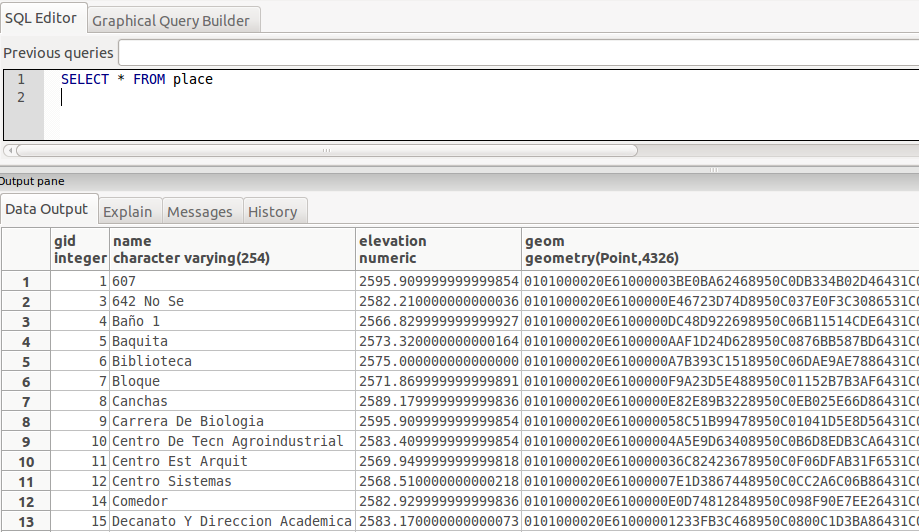
\includegraphics[width=1\textwidth]{iteration1/postgres_places}
           \caption{Herramienta gráfica de PostgreSQL (\emph{pgAdmin}).}
           \label{fig:postgres_places}
           \caption*{Fuente: Elaboración propia}
         \end{center}
       \end{figure}
        % con la tabla de Lugares desplegada.

       En la figura \ref{fig:postgres_places} se puede observar que la columna \emph{Elevation} contiene datos que el GPS Garmin Nuvi 1300 genera al momento de guardar un punto, en el presente caso es irrelevante.\\

       \subsubsection{Las Rutas}
       \label{subs:Las Rutas}

       Después de generar un archivo shapefile en la sección \ref{sec:generar_mapa_rutas}, se procede a popular la base de datos del mismo modo que se hizo con la información de los lugares. Para las rutas se genera una tabla nombrada \emph{ways}.\\

       Posteriormente se procede a preparar la tabla \emph{ways} para que soporte las funciones instaladas por pgRouting.
       % Una vez poblada la base de datos se procede a cargar la misma con la información obtenida en RF011, para tal efecto es necesario primeramente crear una tabla que contendrá los LINESTRING contenidos en el shapefile, esta operación es similar a la realizada en la tarea - RF003 (\ref{sub:RF003}). Una vez que ya se tiene la tabla a la llamamos \emph{ways},
       Es necesario ejecutar un query propio de \emph{pgRouting} el cual tiene como objetivo analizar los datos geo-espaciales de la tabla y añadirle una \emph{topología}.\\

       \begin{verbatim}
         select pgr_createTopology('ways', 0.00000001, 'geom', 'gid');
       \end{verbatim}

       Dentro lo que es la \emph{topología geoespacial} existe una aplicación que se lo conoce como \emph{topología de red}. La \emph{topología de red} representa las relaciones entre segmentos en una red lineal o una colección de segmentos de línea. \cite{osgeo_journal_topology} \\

       En un \emph{SIG} la topología ayuda a mejorar el análisis de datos geo-espaciales, para resolver el problema de la ruta corta \emph{pgRouting} genera una \emph{topología de red} usando los datos que existen en la tabla \emph{ways}, es necesario ejecutar una instrucción, la que se muestra a continuación y \emph{pgRouting} se encarga de llenar los datos que se pueden observar en la figura \ref{fig:postgres_ways}, las columnas \emph{source} y \emph{target} son populadas con el análisis topológico y en la figura \ref{fig:postgres_vertices}, se puede observar que la tabla \emph{ways\_vertices\_pgr} es creada enteramente en la ejecución de la instrucción.\\

       \begin{figure}[H]
         \begin{center}
           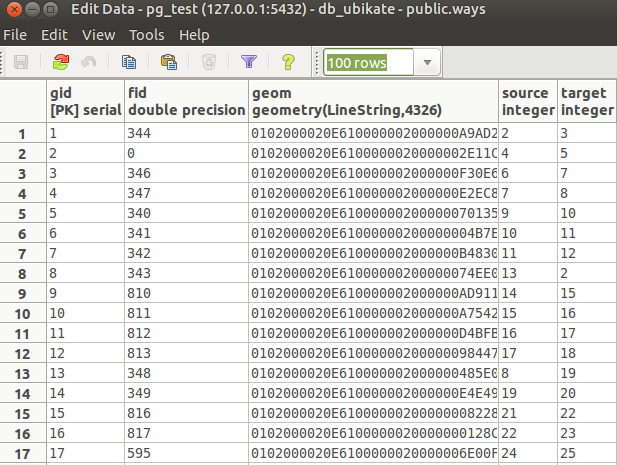
\includegraphics[width=1\textwidth]{iteration2/postgres_ways}
           \caption{Vista de la tabla \emph{ways}.}
           \label{fig:postgres_ways}
           \caption*{Fuente: Elaboración propia}
         \end{center}
       \end{figure}

       En la figura \ref{fig:postgres_ways} se puede apreciar que cada fila es una parte de la línea original obtenida por el dispositivo GPS y explosionada por QGIS, hay que notar que las columnas \emph{source} y \emph{target} hacen referencia a los nodos o vértices que la primera línea tiene en sus extremos, la primera línea o fila está identificada por la columna \emph{gid}.\\

       En la siguiente figura \ref{fig:postgres_vertices} se observa la tabla \emph{ways\_vertices\_pgr} que contiene los vértices creados a partir del análisis de los datos en la tabla \emph{ways}.

       \begin{figure}[H]
         \begin{center}
           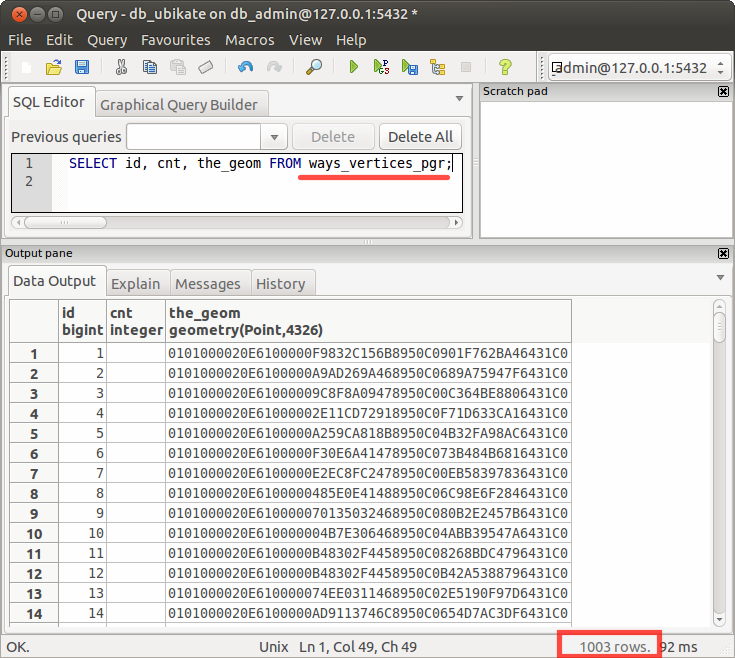
\includegraphics[width=1\textwidth]{iteration2/postgres_vertices}
           \caption{Vista de la tabla \emph{ways\_vertices\_pgr}.}
           \label{fig:postgres_vertices}
           \caption*{Fuente: Elaboración propia}
         \end{center}
       \end{figure}

       Para entender los datos generados hay leer la información de las 2 tablas, por ejemplo en la primera  fila (gid 1) de la tabla \emph{ways}, se observa que el contenido de la columna \emph{source} es igual a \textbf{2} y \emph{target} es igual a \textbf{3}, eso quiere decir que los vértices del LINESTRING de la fila 1 son los vértices con \textbf{id} 2 y 3 respectivamente de la tabla \emph{ways\_vertices\_pgr}.\\


       Todo el conjunto de vértices y líneas de estas tablas se podría representar con una Matriz de adyacencias, explicada en \ref{sub:representacion_de_un_grafo}, y usada en la resolución de la ruta mas corta, mas específicamente con el algoritmo de Dijkstra.\\

       \begin{center}
         \begin{lstlisting}[label=pgr_dijkstra,caption=Algoritmo de Dijkstra implementado en \emph{pgRouting}]
           SELECT seq, id1 AS node, id2 AS edge, cost
           FROM pgr_dijkstra(SELECT gid AS id,
                                     source::integer,
                                     target::integer,
                                     st_length(geom) AS cost
                              FROM public.ways, targetId, sourceId, false, false);
         \end{lstlisting}
       \end{center}


       La anterior consulta SQL es una llamada al método \emph{pgr\_dijkstra} implementado en \emph{pgRouting} el cual solo puede ser utilizado una vez que la base de datos está preparada para tal efecto, es decir necesitamos que la tabla de rutas \emph{ways} tenga la topología de red y también es necesario los ids de los nodos de destino y origen, \emph{targetId} y \emph{sourceId} respectivamente, estos dos últimos datos son obtenidos por una combinación de acciones ya que los nodos son propios del mapa de rutas y el punto destino es en realidad un lugar el cual está ubicado en otra tabla y el punto origen es donde se encuentra el cliente dentro del campus Universitario, por lo tanto una vez obtenido los punto geo-referenciados del lugar de la tabla \emph{places} y el punto donde se encuentra parado el cliente se obtienen los nodos ``más'' cercanos a estos puntos, gracias a que \emph{PostGIS} ya lo tiene implementado, encontrar el nodo más cercano es tan fácil como ejecutar la siguiente consulta SQL, donde \emph{lon} y \emph{lat} son la longitud y latitud del lugar.

       \begin{verbatim}
           SELECT id
           FROM ways_vertices_pgr
           ORDER BY the_geom <-> ST_GeometryFromText('POINT(lon lat)', 4326)
           LIMIT 1
       \end{verbatim}

       Una vez ejecutado el método \emph{pgr\_dijkstra} se obtiene un conjunto de líneas, que son un conjunto de latitudes y longitudes que representa la ruta más corta entre el punto origen y el punto destino, esta informacion realmente no dice nada a la persona que lo lee por lo tanto requiere ser procesada para poder ser consumida desde el navegador, este proceso es llevada a cabo en el servidor y entregada al cliente en formato GeoJSON.\\


       % En la figura XX, se puede ver la tabla \emph{WAYS} con las rutas generadas.





       % Como projected
       % PostGIS maneja dos tipos de datos, geográficos y geométricos

     % section que_se_uso_en_la_aplicacion (end)
 % section sistema_de_coordenadas_para_datos_geograficos (end)
 % \section{Tipo de archivos} % (fold)
 % \label{sec:tipo_de_archivos}
 %
 % section tipo_de_archivos (end)

 % \subsection{Implementaci\'on} % (fold)
 % \label{sub:Implementacion}


   % Para manejar datos georreferenciados con tecnología JavaScript, ya que se implementó el Backend con NodeJS, se hizo uso de la librería \textbf{KnexJS} para manejar la conexión a la base de datos PostgreSQL, y BookshelfJS para las consultas SQL pero para las consultas con datos geoespaciales se realizó a través de esta herramienta pero usando la forma \emph{Raw SQL}\footnote{Raw SQL se refiere a consultas en ``SQL puro'' ya que el fuerte de BookshelfJS es el manejo de las consultas en forma de objetos (ORM), lamentablemente actualmente no existe mucho soporte para manejar datos geoespaciales}.


% Para implementar la comunicación con la base de datos se

% El proyecto

% La estructura de archivos dentro del proyecto \emph{Express} se puede observar en la figura \ref{fig:express_structure}, donde se puede observar las secciones principales de routing, que se encarga de direccionar las peticiones web de acuerdo del protocolo HTTP, la sección de \emph{views} dónde están los templates

% \begin{figure}[H]
%   \begin{center}
%     \caption[Express Application Structure]{Estructura de archivos de una Aplicación \emph{Express}}
%     \label{fig:express_structure}
%     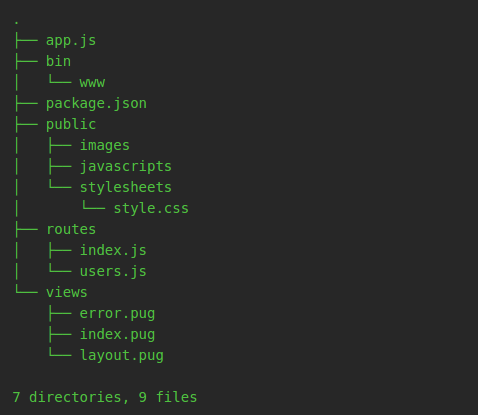
\includegraphics[width=1\textwidth]{express_structure}
%     \caption*{Fuente: https://expressjs.com}
%   \end{center}
% \end{figure}

% Dentro del proyecto \emph{Express} definimos una sección donde localizamos la conexión y las consultas a la base de datos, y otra sección donde



 %
 % Para manejar datos georreferenciados con tecnología JavaScript, ya que se implementó el Backend con NodeJS, se hizo uso de la librería \textbf{KnexJS} para manejar la conexión a la base de datos PostgreSQL, y BookshelfJS para las consultas SQL pero para las consultas con datos geoespaciales se realizó a través de esta herramienta pero usando la forma \emph{Raw SQL}\footnote{Raw SQL se refiere a consultas en ``SQL puro'' ya que el fuerte de BookshelfJS es el manejo de las consultas en forma de objetos (ORM), lamentablemente actualmente no existe mucho soporte para manejar datos geoespaciales}.
 %
 % \begin{center}
 %   \begin{verbatim}
 %     var raw = "SELECT " +
 %                 " ST_AsGeoJSON(geom)::json As geometry," +
 %                 " name," +
 %                 " description," +
 %                 " phone," +
 %                 " level," +
 %                 " gid As id " +
 %               " FROM place WHERE LOWER(name)
 %                      like LOWER('%" + name + "%')";
 %   \end{verbatim}
 % \end{center}

 % De esta forma es que se recupera de la base de datos un lugar georreferenciado, donde este tiene un nombre, una descripción, un teléfono, el nivel o piso donde se encuentra pero lo importante de esta consulta es la obtención del ``punto'' geoespacial del lugar.
 %
 % \begin{center}
 %   \begin{verbatim}
 %     "POINT (-66.14857015827988 -17.394421906929086)"
 %   \end{verbatim}
 % \end{center}
 %
 % % var raw = "SELECT seq, id1 AS node, id2 AS edge, cost
 % %            FROM pgr_dijkstra('SELECT gid AS id,
 % %                                     source::integer,
 % %                                     target::integer,
 % %                                     st_length(geom) AS cost
 % %                               FROM public.ways', targetId, sourceId, false, false);";
 %
 %
 %  Este atributo es de tipo \emph{punto} \'o \emph{point} el cual tiene un \emph{SRID}\footnote{ Spatial Reference System Identifier, El \emph{SRID} corresponde a un sistema de referencia espacial basado en el elipsoide concreto usado para la creación de mapas de tierra plana o de tierra redonda.\cite{msdn_srid} } \emph{3857}\footnote{La proyección Mercator usa el EPSG 3857}, el SRID  es la llave primaria de la tabla \emph{spatial\_ref\_sys} que se crea cuando se inicializa una base de datos que soporte informacion geoespacial (PostGis), esta tabla provee la información necesaria para interpretar y convertir correctamente todas las coordenadas existentes, el \emph{SRID 3857} está definida en la tabla \emph{spatial\_ref\_sys} como ``Popular Visualisation CRS / Mercator''.\\


 Obtener la coordenada es el primer paso, seguidamente se debe mostrarlo sobre un mapa, en este caso \emph{Open Street Maps}, como se puede apreciar en la figura \ref{fig:ember_leaflet}, esta interfaz está implementada usando \emph{ember-leaflet}, el cual está principalmente dise\~nada para ofrecer una mejor experiencia de usuario en celulares smartphones.\\

 % \begin{center}
 %   \begin{verbatim}
 %     var maker = new google.maps.Marker({
 %       position: new google.maps.LatLng( lat, lng  )
 %       map: UMSS.map
 %     });
 %   \end{verbatim}
 % \end{center}

 \begin{verbatim}
   {{#leaflet-map lat=lat lng=lng zoom=zoom}}
     {{tile-layer url="http://{s}.tile.openstreetmap.fr/hot/{z}/{x}/{y}.png" }}
       {{#marker-layer location=location}}
         <h3>{{model.name}}</h3>
         {{model.description}} <br>
         <strong>telf:</strong> {{model.phone}} <br>
         <strong>piso </strong>#{{model.level}}
     {{/marker-layer}}
   {{/leaflet-map}}
 \end{verbatim}

 \begin{figure}[H]
       \begin{center}
         \caption{\emph{ember-leaflet} nos ayuda a desplegar un mapa y mostrar un \emph{punto} o \emph{lugar} con un \emph{marcador} y dibuja una línea de color rojo sobre el mapa.}
         \label{fig:ember_leaflet}
         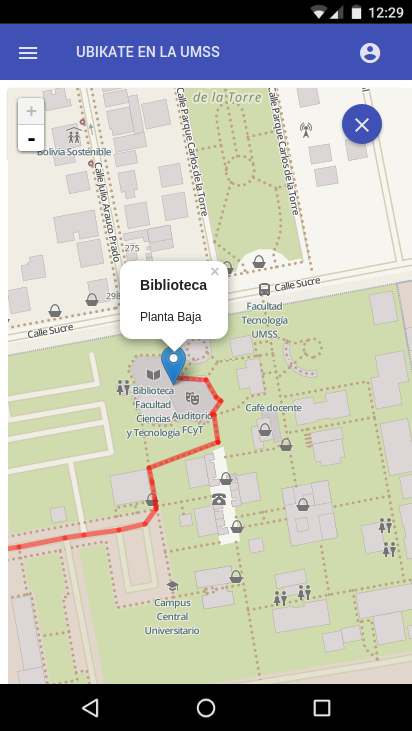
\includegraphics[width=0.5\textwidth]{ember_leaflet}
       \end{center}
       \caption*{Fuente: Elaboración propia.}
 \end{figure}


\section{Crear el Frontend}
\label{sec:Crear el Frontend}


El frontend como ya se mencionó es la vista de la aplicación, es donde el usuario interactúa con la aplicación, en el presente proyecto se implementó usando \emph{Ember.JS}, el cual es un framework de desarrollo JavaScript orientado a crear Aplicaciones de Página Única, esto quiere decir que una vez que se carge la pagina la primera vez ya no se recargara la pagina como tal, en cambio se actualizará de acuerdo como el usuario interactúa con la aplicación.\\

Ya que el proyecto se enfocara en la creación de una aplicación web optimizada para su uso en celulares, es primordial que el ``look and feel'' de la aplicación sea lo más parecido a una aplicación móvil nativa, para lograr este efecto se utilizó \emph{ember-paper}, que ya trae implementado componentes (botones, listas, links, menús de navegación, etc.) con un comportamiento que emula a una aplicación móvil nativa.\\

% Para empezar esta tarea se procedió a instalar y configurar el framework de desarrollo Ember JS, que nos ayudará en la implementación del frontend de la aplicación o la capa que interactúa con el usuaria, y Express JS, el cual manejara el backend de la aplicación, básicamente se encarga de la lógica del sistema y la comunicación con la base de datos.\\

\emph{EmberJS} está basado en ``Convención sobre Configuración'', ya que la gran mayoría de los problemas con que uno se puede enfrentar a la hora de crear una aplicación web ya fueron resueltas por la comunidad de desarrollo, por lo tanto ya se llegó a un patrón o convención de cómo se debería resolver algún determinado problema, \emph{EmberJS} implementa y sugiere soluciones a problemas comunes, para que de esa forma el desarrollo no se enfoque  en resolver problemas ya resueltos (configuración) si no en implementar en la lógica del negocio de la aplicación, que al final es lo que le da valor al producto que queremos desarrollar y también para que si en un futuro otro desarrollador empieza a trabajar en el proyecto, sea capaz de entender la estructura y el diseño de la aplicación de forma sencilla. Por lo tanto nos enfocaremos en analizar cómo se resolvieron los problemas: de cómo mostrar los lugares, geolocalizar el lugar sobre un mapa, mostrar la ruta más corta dentro del campus Universitario, manejo de los usuario y como mostrar el reporte de los lugares más visitados.

\subsection{Mostrar los Lugares}
\label{sub:Mostrar los Lugares}




%
% Para empezar esta tarea se procedió a instalar \emph{Ember.JS}, que al ser un paquete \emph{Node.JS} solo es necesario ejecutar el siguiente comando.
%
% \begin{verbatim}
%   $ npm install -g ember-cli
% \end{verbatim}
%
% Posteriormente se puede observar


Durante la investigación de esta tarea se encontró \emph{ember-leaflet}, una librería o plugin que contiene las herramientas para poder cargar y usar un servicio de mapas.\\

Para instalar esta librería solo se necesita ejecutar el siguiente comando y posteriormente ya se puede empezar a utilizarla.\\

\begin{verbatim}
 $ ember install ember-leaflet
\end{verbatim}

El resultado de la investigación puede apreciar en el marco teórico, en la sección que describe la librería, \emph{ember-leaflet}. \ref{sec:ember_js}





\begin{figure}[H]
 \begin{center}
   \caption{Vista de la lista de Lugares registrados en el sistema.}
   \label{fig:places_index}
   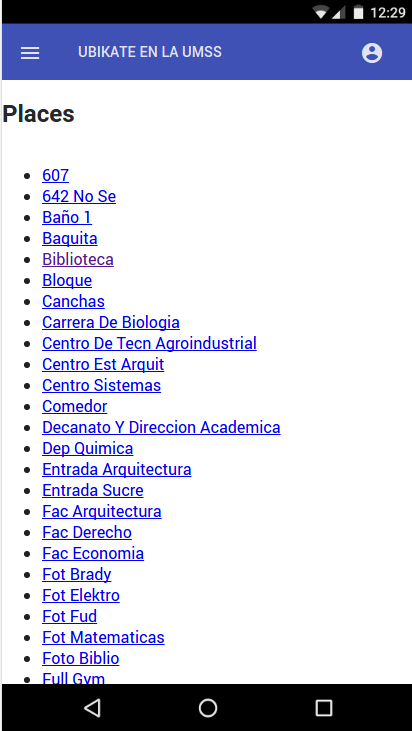
\includegraphics[width=0.5\textwidth]{iteration1/places_index}
   \caption*{Fuente: Elaboración propia}
 \end{center}
\end{figure}


\begin{figure}[H]
 \begin{center}
   \caption{Vista de la búsqueda de lugares a través de un cajón de búsqueda.}
   \label{fig:places_search}
   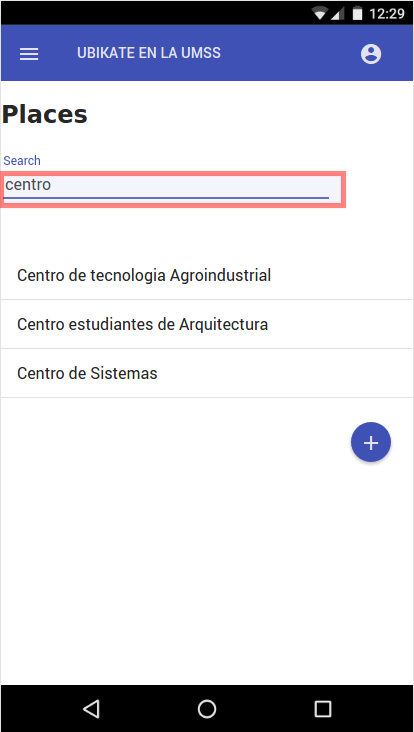
\includegraphics[width=0.5\textwidth]{iteration1/places_search}
   \caption*{Fuente: Elaboración propia}
 \end{center}
\end{figure}


Para implementar esta funcionalidad del sistema fue necesario utilizar las funcionalidad de Ember JS.

\begin{verbatim}
 {{#paper-item class="md-1-line" onClick=(transition-to 'places.show' place)}}
     <div class="md-list-item-text">
         <span>{{place.name}}</span>
     </div>
 {{/paper-item}}
\end{verbatim}


\begin{figure}[H]
   \label{fig:place_show}
   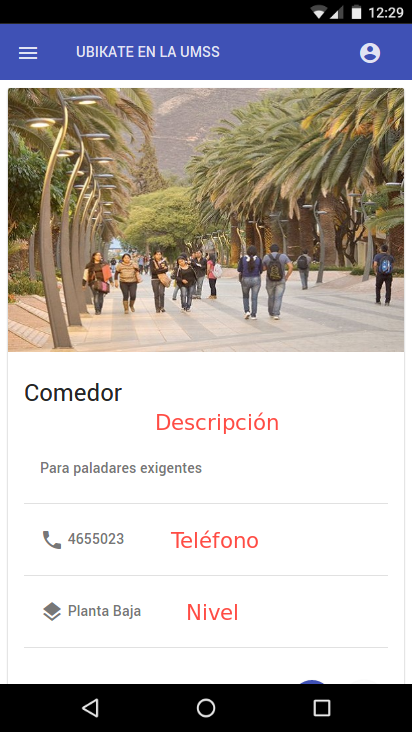
\includegraphics[width=0.5\textwidth]{iteration1/place_show}
   \caption*{Fuente: Elaboración propia}
 \end{center}
\end{figure}





\subsection{Mostrar los Rutas}
\label{sub:Mostrar los Rutas}


\subsection{Manejo de Usuarios}
\label{sub:Manejo de Usuarios}



\section{Informe de los datos}
\label{sec:Informe de los datos}

  \chapter{Desarrollo}
\label{chap:desarrollo}



En el presente proyecto se implementó una aplicación web móvil, como ya se explico, este tipo de aplicaciones son básicamente páginas web, con amplia funcionalidad e implementadas específicamente para su uso en dispositivos móviles, tablets o smartphones, para lo cual se investigó las tecnologías, arquitecturas y los frameworks de desarrollo que actualmente usan este tipo de aplicaciones, una de los concepto que se estudió fue de las \emph{aplicaciones de página única}, concepto que se empezó a discutir a principios de 2003, y se puso de moda con la aparición de frameworks JavaScript que agilizan y facilitan en gran medida la implementación de aplicaciones web, tales como \emph{AngularJS}, \emph{BackboneJS} y en el 2010 \emph{EmberJS}. \\

Es necesario reconocer las diferentes partes con la que cuenta una aplicación web móvil como una aplicación de página única diseñada para dispositivos móviles, es necesario implementar un REST API que se encargue de hacer las consultas a la base de datos y que el cliente pueda consumir la información obtenida de la base de datos así como también el camino inverso, la base de datos necesita manejar informacion geoespacial y el cliente necesita que la aplicación sea optimizada para su uso en dispositivos móviles. Tomando en cuenta estos requerimientos se puede separar el desarrollo del proyecto en los siguientes apartados. \\


\section{Iteración 1}
\label{sec:iteracion_1}

% Para la primera iteración se implementaron las historias de usuario con más relevancia dentro de la lógica de negocio del cliente, estas son generalmente las que tienen mayor impacto en el sistema a desarrollar. \\

%
% \subsection{Iteration Planning Meeting}
% \label{sub:Iteration Planning Meeting}

\subsection{Planificación}

En esta etapa se analizaran las Historias de Usuario seleccionadas para esta iteración, y se las dividirá en \emph{tareas de ingeniería}. \\

% \begin{itemize}
%   \item \textbf{Planificación de la Iteración 1:} En esta etapa se analizan las Historias de Usuario seleccionadas para esta iteración, y se las divide en \emph{tareas de ingeniería}.
% \end{itemize}
  %
  % \subsection{Exploración y Planeación}
  % \label{subs:Exploración y Planeación}


% En un equipo de desarrollo formado por varias personas, las fases de Exploración y Planeación se las realiza por separado, primeramente en la fase de \emph{exploración} los desarrolladores se apropian de alguna de las historias de usuario planeadas para la iteración y procede a dividir la historia de usuario en \emph{Tareas de Ingeniería}, posteriormente en la fase de la \emph{Planeación}, todos los desarrolladores estiman las tareas de acuerdo a criterio propio. \\
%
% Tomando en cuenta que el equipo de desarrollo está compuesto solo por mi persona, para la implementación del presente proyecto de grado, las fases de Exploración y Planeación se las realizó al mismo tiempo. \\
%
% Para la primera iteración se determinó que las historias de usuario a implementar serían la 1 y la 2.   \\
% %
% Posteriormente como tarea del desarrollador se procede a dividir las historias de usuario en Tareas de Ingeniería, en la tabla se determinaron las Tareas pertenecientes a la historia de usuario 2, dentro lo que es la planeación se debe repartir las tareas entre los desarrolladores, pero ya que el equipo de desarrollo se traduce a mi persona, todas las tareas recaen sobre mi responsabilidad, como parte de la planeación es necesario estimar las tareas,

% En esta etapa se analizan las Historias de Usuario seleccionadas para esta iteración, y se las divide en \emph{tareas de ingeniería}.

  % \subsubsection{Tareas del US01}
  % \label{sub:us01_tasks}

En primer lugar se analizará la \emph{historia de usuario} US01, tal como se puede ver en el cuadro \ref{tab:US01}.

  
\begin{table}[H]
  \begin{center}
    \begin{tabularx}{0.75\textwidth}{ X }
      \toprule
      \textbf{Historia de Usuario:} US01
      \makebox[6cm][r]{\textbf{Prioridad:} Alta \space} \\
      \makebox[4cm][r]{}
      \makebox[6cm][r]{\textbf{Riesgo:} Medio} \\
      \textbf{Nombre:} Implementar la lista de lugares.\\

      % \textbf{Prioridad:} Alta \\
      % \textbf{Riesgo:} Alta \\

      % \addlinespace
      % \textbf{Nombre:} Verificar el Formulario de Registro \\

      \addlinespace
      \textbf{Descripción:} \\
      \tab Yo como visitante\\
      \tab Deseo ver una lista de lugares \\
      % & Deseo ingresar el nombre de un lugar\\
      \tab Para encontrar el lugar al que deseo ir\\

      \addlinespace
      \textbf{Criterios de Aceptación:} \\
      \tab Quiero tener los lugares en una base de datos \\
      \tab Quiero ver una lista de lugares\\
      \tab Quiero filtrar la lista de lugares por el nombre o parte de este\\

      \bottomrule
    \end{tabularx}
    \caption{Historia de Usuario - US01}
    \label{tab:US01}
  \end{center}
\end{table}


    \begin{table}[H]
  \begin{center}
    \begin{tabularx}{0.75\textwidth}{ X }
      \toprule
      \textbf{Número de Tarea:} T001
      \makebox[1cm][r]{}
      \makebox[6cm][r]{\textbf{Historia de Usuario:} US01} \\

      \addlinespace
      \textbf{Descripción:} Crear un archivo shapefile con información inicial de lugares principales dentro el campus de la UMSS. \\

      \addlinespace
      \textbf{Tipo de Tarea:} Desarrollo
      % \makebox[1cm][r]{}
      \makebox[6cm][r]{\textbf{Estimación [dias]:} 1} \\

      \addlinespace
      \textbf{Programador Responsable:} Edmundo Figueroa \\

      \bottomrule
    \end{tabularx}
    \caption{Tarea de Ingeniería - T001}
    \label{tab:T001}
  \end{center}
\end{table}


\begin{table}[H]
  \begin{center}
    \begin{tabularx}{0.75\textwidth}{ X }
      \toprule
      \textbf{Número de Tarea:} T002
      \makebox[1cm][r]{}
      \makebox[6cm][r]{\textbf{Historia de Usuario:} US01} \\

      \addlinespace
      \textbf{Descripción:} Crear una base de datos que pueda manejar información geoespacial. \\

      \addlinespace
      \textbf{Tipo de Tarea:} Desarrollo
      % \makebox[1cm][r]{}
      \makebox[6cm][r]{\textbf{Estimación [dias]:} 1} \\

      \addlinespace
      \textbf{Programador Responsable:} Edmundo Figueroa \\

      \bottomrule
    \end{tabularx}
    \caption{Tarea de Ingeniería - T002}
    \label{tab:T002}
  \end{center}
\end{table}

\begin{table}[H]
  \begin{center}
    \begin{tabularx}{0.75\textwidth}{ X }
      \toprule
      \textbf{Número de Tarea:} T003
      \makebox[1cm][r]{}
      \makebox[6cm][r]{\textbf{Historia de Usuario:} US01} \\

      \addlinespace
      \textbf{Descripción:} Popular la base de datos creada en T002 con la información de T001. \\

      \addlinespace
      \textbf{Tipo de Tarea:} Desarrollo
      \makebox[6cm][r]{\textbf{Estimación [dias]:} 0.5} \\

      \addlinespace
      \textbf{Programador Responsable:} Edmundo Figueroa \\

      \bottomrule
    \end{tabularx}
    \caption{Tarea de Ingeniería - T003}
    \label{tab:T003}
  \end{center}
\end{table}

\begin{table}[H]
  \begin{center}
    \begin{tabularx}{0.75\textwidth}{ X }
      \toprule
      \textbf{Número de Tarea:} T004
      \makebox[1cm][r]{}
      \makebox[6cm][r]{\textbf{Historia de Usuario:} US01} \\

      \addlinespace
      \textbf{Descripción:} Mostrar una lista de los lugares. \\

      \addlinespace
      \textbf{Tipo de Tarea:} Desarrollo
      \makebox[6cm][r]{\textbf{Estimación [dias]:} 2} \\

      \addlinespace
      \textbf{Programador Responsable:} Edmundo Figueroa \\

      \bottomrule
    \end{tabularx}
    \caption{Tarea de Ingeniería - T004}
    \label{tab:T004}
  \end{center}
\end{table}


\begin{table}[H]
  \begin{center}
    \begin{tabularx}{0.75\textwidth}{ X }
      \toprule
      \textbf{Número de Tarea:} T005
      \makebox[1cm][r]{}
      \makebox[6cm][r]{\textbf{Historia de Usuario:} US01} \\

      \addlinespace
      \textbf{Descripción:} Filtrar los lugares ingresando el nombre o parte de este. \\

      \addlinespace
      \textbf{Tipo de Tarea:} Desarrollo
      \makebox[6cm][r]{\textbf{Estimación [dias]:} 1} \\

      \addlinespace
      \textbf{Programador Responsable:} Edmundo Figueroa \\

      \bottomrule
    \end{tabularx}
    \caption{Tarea de Ingeniería - T005}
    \label{tab:T005}
  \end{center}
\end{table}


  % \subsubsection{Tareas del US02}
  % \label{sub:us02_tasks}

Posteriormente se analizará la la \emph{historia de usuario} US02, ver el cuadro \ref{tab:US02}.

  
\begin{table}[H]
 \begin{center}
   \begin{tabularx}{0.75\textwidth}{ X }
     \toprule
     \textbf{Historia de Usuario:} US02
     \makebox[6cm][r]{\textbf{Prioridad:} Baja} \\
     \makebox[4cm][r]{}
     \makebox[6cm][r]{\textbf{Riesgo:} Alto} \\

     \addlinespace
     \textbf{Nombre:} Implementar la vista de la información del lugar.\\
     
     \addlinespace
     \textbf{Descripción:} \\
     \tab Yo como visitante\\
     \tab Deseo ver la información de un lugar\\
     % & Deseo ingresar el nombre de un lugar\\
     \tab Para decidir si es el lugar que estoy buscando\\

     \addlinespace
     \textbf{Criterios de Aceptación:} \\
     \tab Quiero leer una descripción del lugar \\
     \tab Quiero ver un teléfono asociado al lugar\\
     \tab Quiero ver en qué piso se encuentra el lugar\\

     \bottomrule
   \end{tabularx}
   \caption{Historia de Usuario - US02}
   \label{tab:US02}
 \end{center}
\end{table}


    \begin{table}[H]
  \begin{center}
    \begin{tabularx}{0.75\textwidth}{ X }
      \toprule
      \textbf{Número de Tarea:} T006
      \makebox[1cm][r]{}
      \makebox[6cm][r]{\textbf{Historia de Usuario:} US02} \\

      \addlinespace
      \textbf{Descripción:} Mostrar la Descripcion del lugar. \\

      \addlinespace
      \textbf{Tipo de Tarea:} Desarrollo
      \makebox[6cm][r]{\textbf{Estimación [dias]:} 0.5} \\

      \addlinespace
      \textbf{Programador Responsable:} Edmundo Figueroa \\

      \bottomrule
    \end{tabularx}
    \caption{Tarea de Ingeniería - T006}
    \label{tab:T006}
  \end{center}
\end{table}


\begin{table}[H]
  \begin{center}
    \begin{tabularx}{0.75\textwidth}{ X }
      \toprule
      \textbf{Número de Tarea:} T007
      \makebox[1cm][r]{}
      \makebox[6cm][r]{\textbf{Historia de Usuario:} US02} \\

      \addlinespace
      \textbf{Descripción:} Mostrar el telefono del lugar. \\

      \addlinespace
      \textbf{Tipo de Tarea:} Desarrollo
      % \makebox[1cm][r]{}
      \makebox[6cm][r]{\textbf{Estimación [dias]:} 0.5} \\

      \addlinespace
      \textbf{Programador Responsable:} Edmundo Figueroa \\

      \bottomrule
    \end{tabularx}
    \caption{Tarea de Ingeniería - T007}
    \label{tab:T007}
  \end{center}
\end{table}

\begin{table}[H]
  \begin{center}
    \begin{tabularx}{0.75\textwidth}{ X }
      \toprule
      \textbf{Número de Tarea:} T008
      \makebox[1cm][r]{}
      \makebox[6cm][r]{\textbf{Historia de Usuario:} US02} \\

      \addlinespace
      \textbf{Descripción:} Mostrar el nivel o el piso del lugar. \\

      \addlinespace
      \textbf{Tipo de Tarea:} Desarrollo
      \makebox[6cm][r]{\textbf{Estimación [dias]:} 0.5} \\

      \addlinespace
      \textbf{Programador Responsable:} Edmundo Figueroa \\

      \bottomrule
    \end{tabularx}
    \caption{Tarea de Ingeniería - T008}
    \label{tab:T008}
  \end{center}
\end{table}

\begin{table}[H]
  \begin{center}
    \begin{tabularx}{0.75\textwidth}{ X }
      \toprule
      \textbf{Número de Tarea:} T009
      \makebox[1cm][r]{}
      \makebox[6cm][r]{\textbf{Historia de Usuario:} US02} \\

      \addlinespace
      \textbf{Descripción:} Mostrar una imagen o foto del lugar. \\

      \addlinespace
      \textbf{Tipo de Tarea:} Desarrollo
      \makebox[6cm][r]{\textbf{Estimación [dias]:} 2} \\

      \addlinespace
      \textbf{Programador Responsable:} Edmundo Figueroa \\

      \bottomrule
    \end{tabularx}
    \caption{Tarea de Ingeniería - T009}
    \label{tab:T009}
  \end{center}
\end{table}


    %
    % \begin{itemize}
    %   \item \textbf{Implementación de la Iteración 1:}
    % \end{itemize}




\subsection{Diseño}


\begin{itemize}
  \item \textbf{Diagrama Entidad - Relación:}

En la figura \ref{fig:er_lugar}, se observa el diagrama Entidad - Relación correspondiente a los \emph{lugares} dentro del campus Universitario.

\begin{figure}[H]
  \begin{center}
    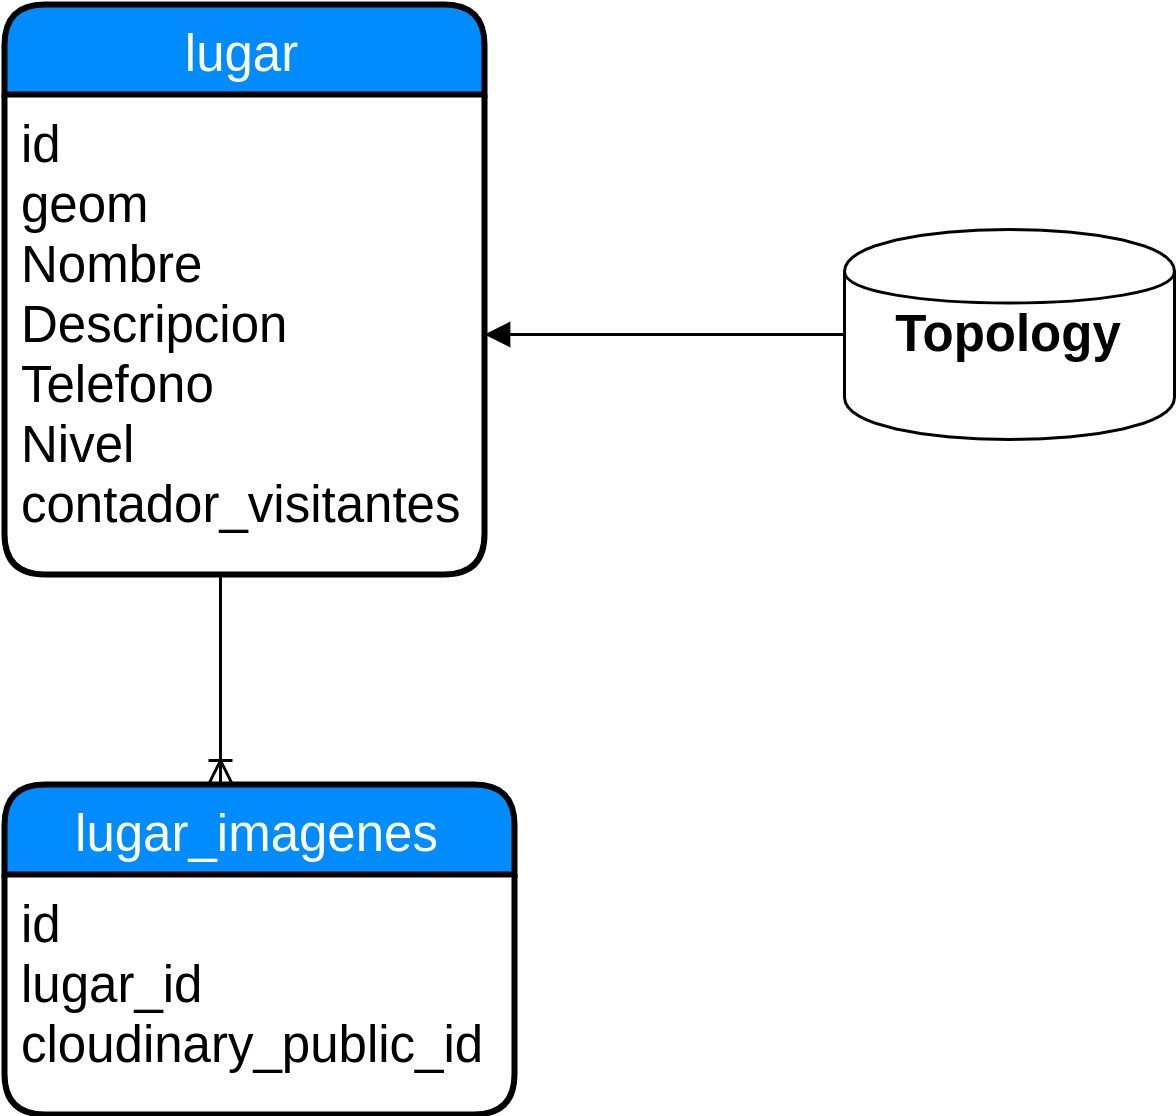
\includegraphics[width=0.4\textwidth]{diagramas/er_lugar}
  \end{center}
  \caption{Diagrama ER: Lugares}
  \label{fig:er_lugar}
  \caption*{Fuente: Elaboración propia}
\end{figure}



\item \textbf{Diagrama de Secuencia:}

En la figura \ref{fig:sequence_ver_lugar}, se observa el diagrama de secuencia correspondiente obtención de la lista e información de lugares.


\begin{figure}[H]
  \begin{center}
    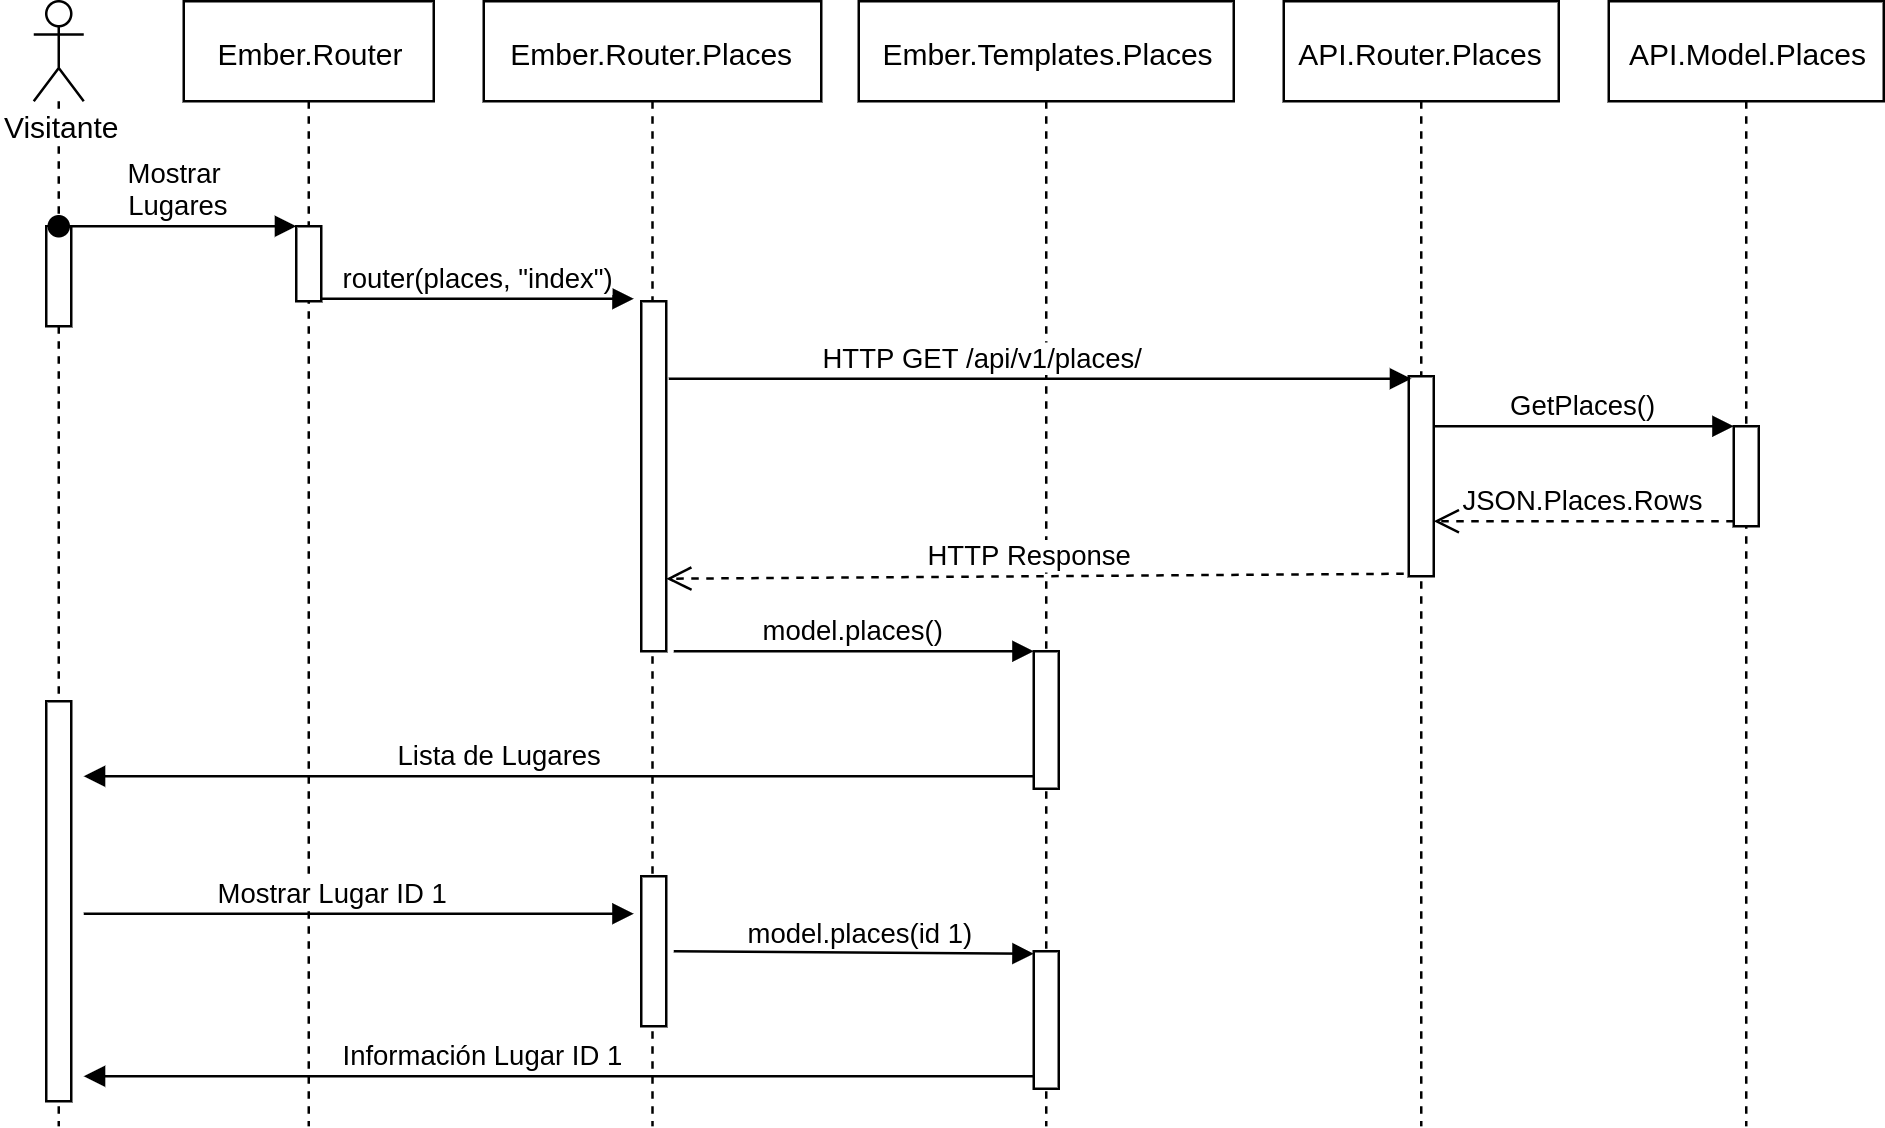
\includegraphics[width=0.9\textwidth]{diagramas/sequence_ver_lugar}
  \end{center}
  \caption{Diagrama de Secuencia: Lista e Información de Lugares}
  \label{fig:sequence_ver_lugar}
  \caption*{Fuente: Elaboración propia}
\end{figure}



\item \textbf{Diagrama de Clases:}


En la figura \ref{fig:clases_lugares}, se observa el diagrama de clases correspondiente a los lugares y la información de estos.

\begin{figure}[H]
\begin{center}
  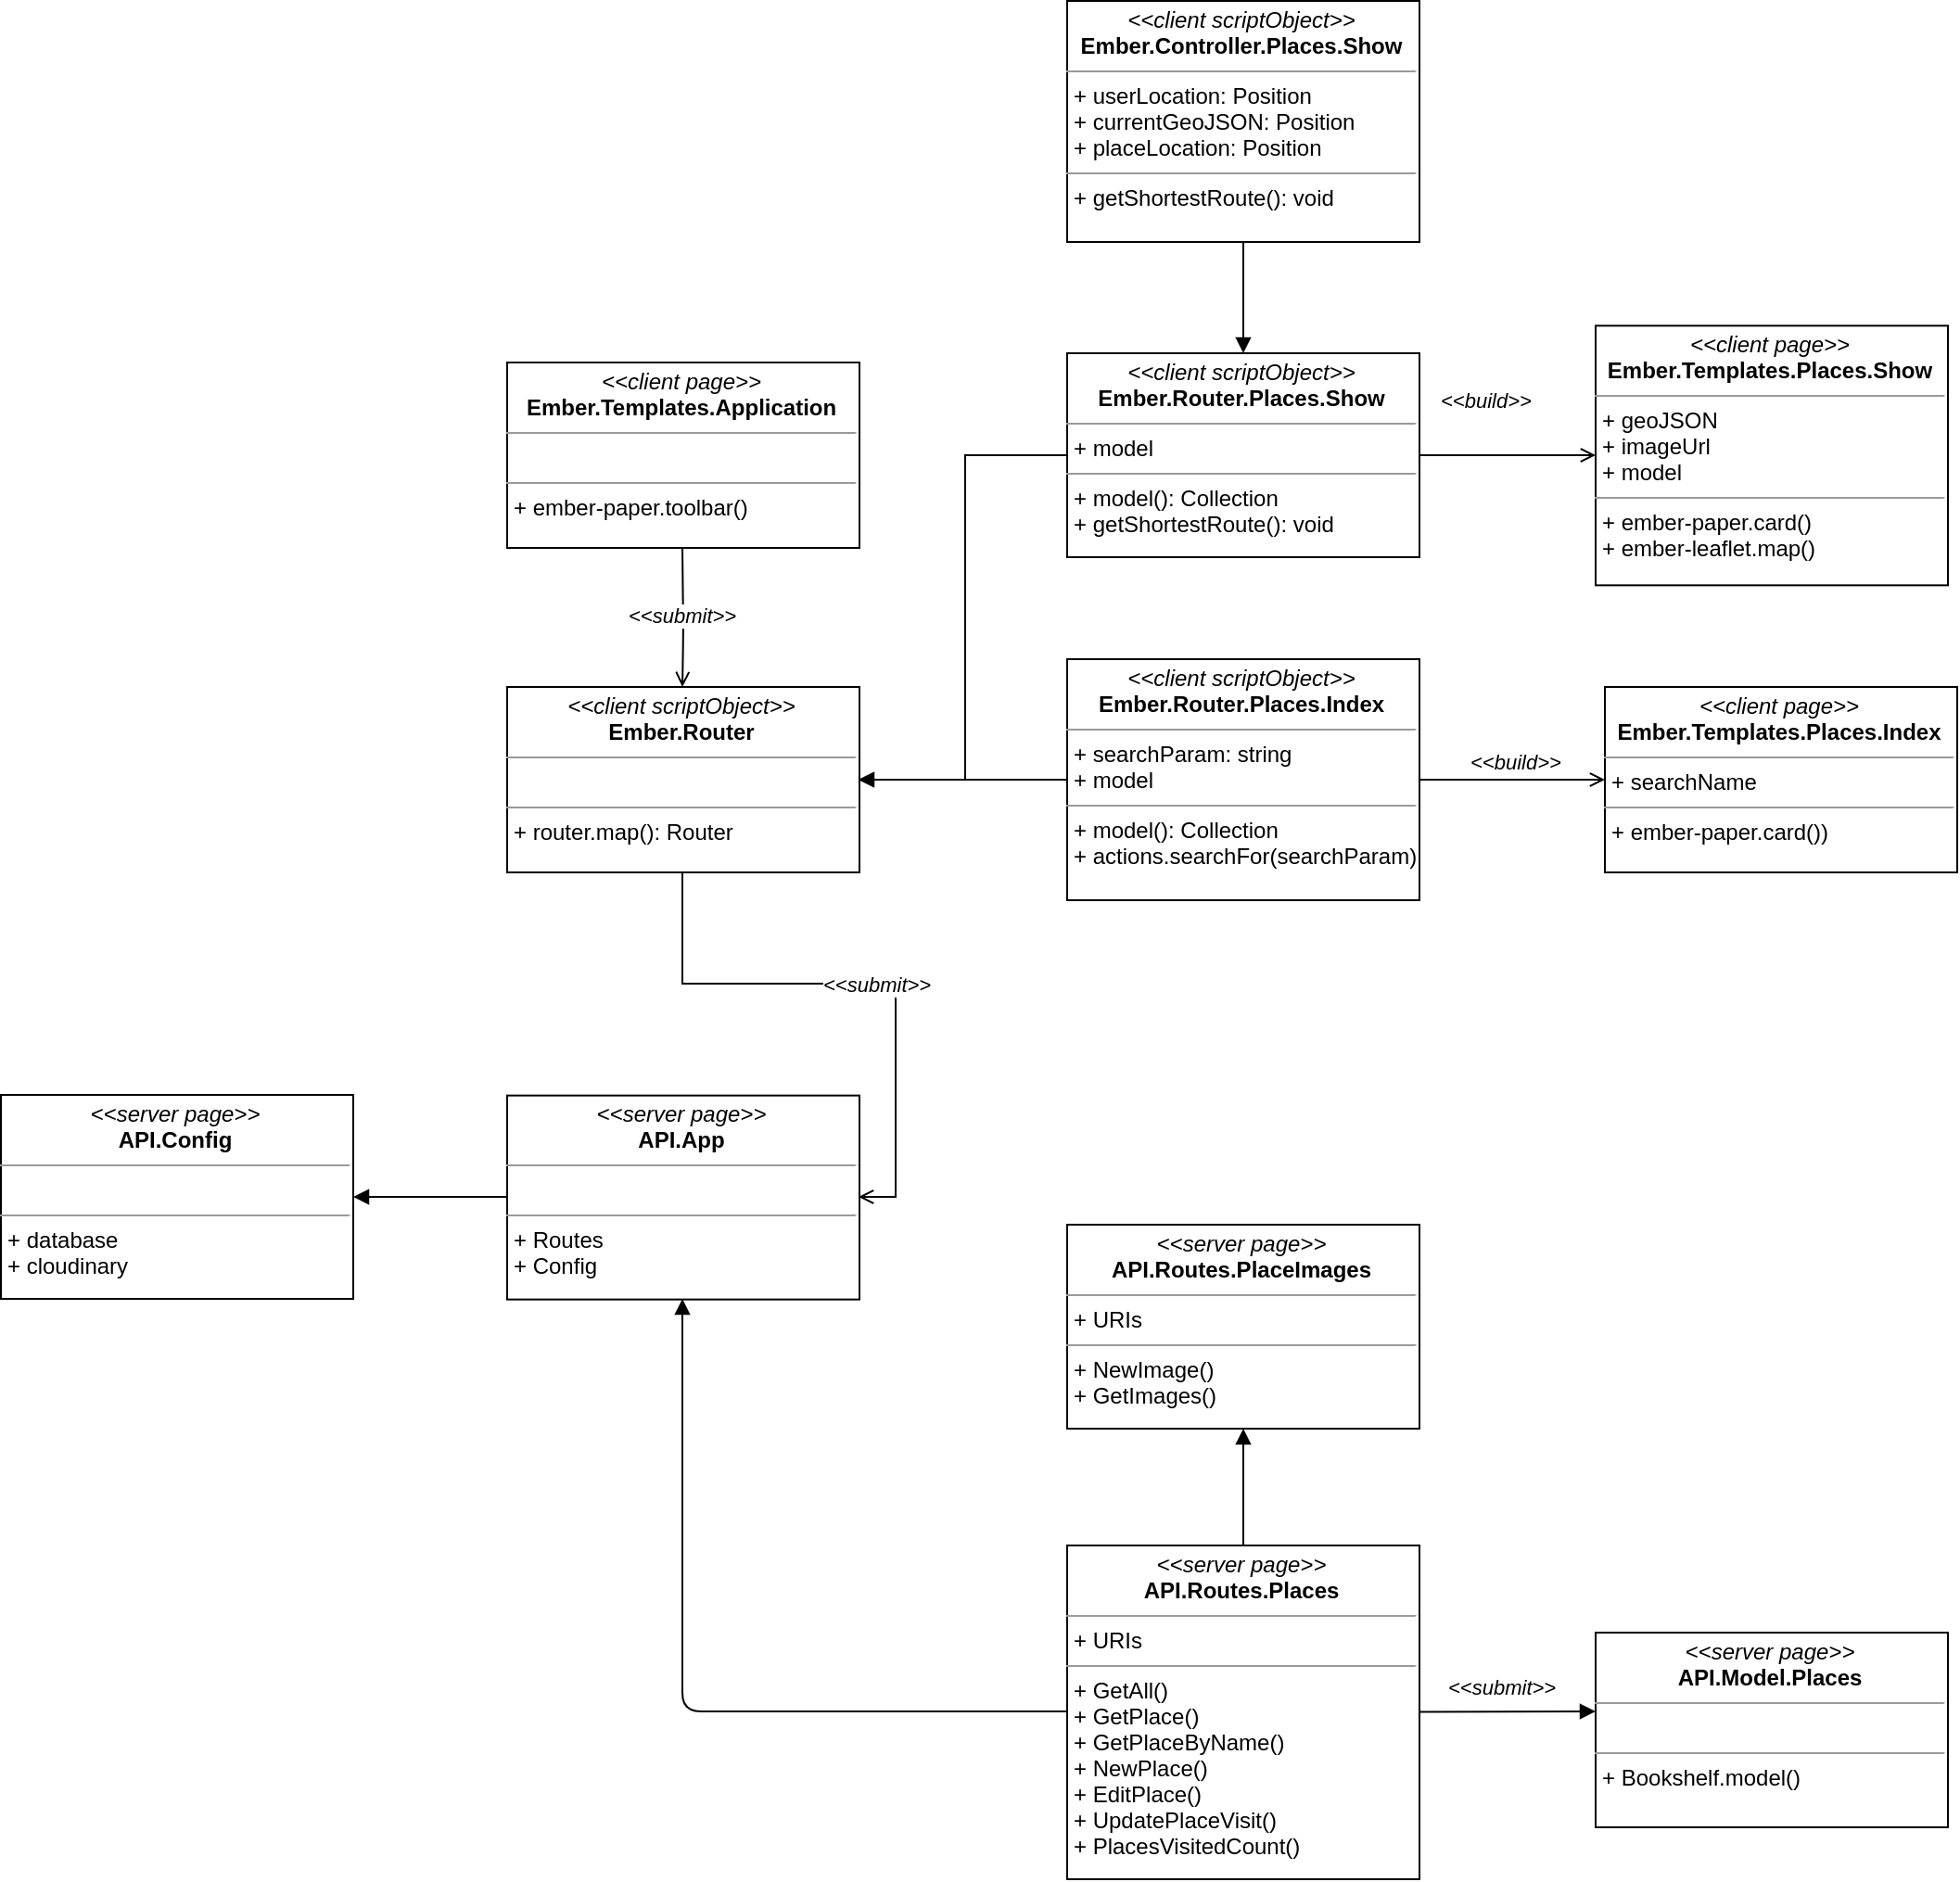
\includegraphics[width=0.9\textwidth]{diagramas/clases_lugares}
\end{center}
\caption{Diagrama de Clases: Lugares}
\label{fig:clases_lugares}
\caption*{Fuente: Elaboración propia}
\end{figure}


\end{itemize}


\subsection{Implementación}
% \label{sub:implementacion_iteracion_1}

    \subsubsection{Recolecion de la informacion de los lugares}
% \label{subs:Los lugares}

En primer lugar se recolectó la información de los lugares que la aplicación contendrá  de forma inicial, al igual que para recolectar las rutas se hizo uso de un \emph{GPS Garmin Nuvi 1300}, el cual cuenta con la opción de guardar locaciones como favoritos, entonces solo fue necesario estar cerca del lugar que se desea guardar y activar esa opción del GPS, este guarda la información en un archivo \emph{.gpx} y con la ayuda de \emph{QGIS} se genero el archivo shapefile correspondiente.\\

Posteriormente es necesario pasar la información geoespacial del shapefile a la base de datos, para esta tarea se hizo uso de una herramienta disponible para postgres, \emph{shp2pgsql}, que permite la conversión de un archivo shapefile a un archivo sql.

% $ shp2pgsql -s 4326 -I -S -c -d ~/Documents/places.shp > places.sql
\begin{verbatim}
  $ shp2pgsql -s 3785 -I -S -c -d ~/Documents/places.shp > places.sql
\end{verbatim}

Con el anterior comando se tiene como resultado un archivo \emph{.sql}, el cual es ingresado en la base de datos ya configurada, de esta forma nuestra base de datos para a contener una tabla geoespacial con datos de tipo \emph{POINT}, los cuales representan los lugares dentro del campus de la UMSS.\\

% \begin{verbatim}
%   $ shp2pgsql -s 4326 -I -S -c -d ~/Documents/ways.shp > ways.sql
% \end{verbatim}
%
% De la misma forma es necesario pasar la información de las rutas contenidas en un archivo shapefile a un archivo sql, en este caso creará una tabla \emph{WAYS}.\\

El archivo \emph{sql} resultante es usado para popular la base de datos con la información inicial de los lugares que contiene el campus universitario, para tal tarea se usó el siguiente comando.\\
% Los archivos resultantes \emph{sql} son usados para popular la base de datos .\\

\begin{verbatim}
  $ psql -d db_ubikate -U db_admin -f /Documents/places.sql
\end{verbatim}

\begin{figure}[H]
  \begin{center}
    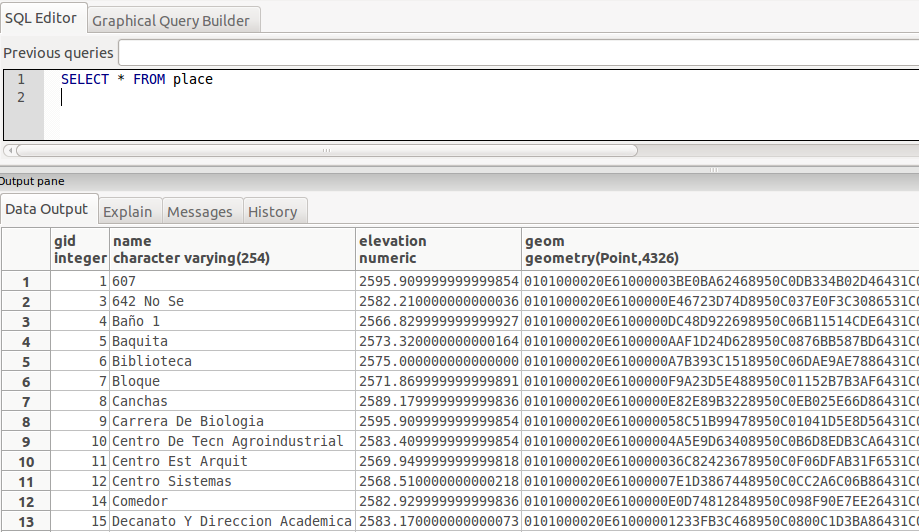
\includegraphics[width=1\textwidth]{iteration1/postgres_places}
    \caption{Herramienta gráfica de PostgreSQL (\emph{pgAdmin}).}
    \label{fig:postgres_places}
    \caption*{Fuente: Elaboración propia}
  \end{center}
\end{figure}
 % con la tabla de Lugares desplegada.

En la figura \ref{fig:postgres_places} se puede observar que la columna \emph{Elevation} contiene datos que el GPS Garmin Nuvi 1300 genera al momento de guardar un punto, en el presente caso es irrelevante.\\


Una vez que se tiene populada la base de datos con la informacion de los lugares es necesario implementar el como se comunicara el backend con el frontend, este como ya se explico se implementara un Servicio Web basado en un API REST.\\



\subsubsection{Implementación del REST API}
\label{subs:Implementacion del REST API}



El servidor necesita reconocer las peticiones que le llegan del cliente, para lo cual es necesario ``mapear'' un URI a una acción específica, las cuales ya están preparadas para comunicarse con la base de datos, no hay restricción en la declaración de las URIs pero para una mejor comprensión del API que se está desarrollando es necesario seguir convenciones que aseguran que cualquier desarrollador pueda comprender el API presentado y pueda ser fácilmente consumido por cualquier aplicación que requiera acceder a la información que disponible, un API REST es el que cumple con estas características.
En primer lugar es necesario crear las URIs que serán ``entendidas'' por el servidor, esto se logra declarando en el servicio creado con \emph{Express.JS}, tal como se puede apreciar en el siguiente bloque de código, cada URI se lo relaciona a un modelo en específico de acuerdo a la acción que se requiere, tal como se puede observar en el cuadro \ref{tab:rest} las URIs declaradas en el API cumplen con tal característica.\\


% \begin{minted}{js}[label=express_api,caption=Declarando API REST con ExpressJS]
\begin{center}
  \begin{lstlisting}[label=express_api,caption=Declarando API REST con ExpressJS]

        const router = express.Router();
        router.get('/', places.getAll);
        router.get('/:id', places.getPlace);
        router.post('/', places.newPlace);
        router.put('/:id', places.editPlace);
        router.delete('/:id', places.deletePlace);

        app.use('/api/v1/places', router);

  \end{lstlisting}
\end{center}
% \end{minted}

% En el código

  %
  % Para lograr todo este comportamiento  es necesario declarar, en el archivo
  % que controla las rutas dentro de la aplicación, \textbf{routes}, que el
  % recurso \textbf{user} es \emph{restful}, tal como se muestra en la figura \ref{fig:rest}\\

  % \begin{figure}[!hbp]
  %   \begin{center}
  %     \caption[REST - routes.rb]{config/routes.rb}
  %     \label{fig:rest}
  %     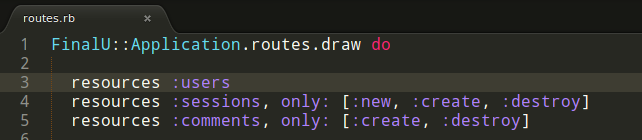
\includegraphics[width=1\textwidth]{rest}
  %     \caption*{Fuente: }
  %   \end{center}
  % \end{figure}

  El cuadro \ref{tab:rest} muestra como se puede leer las peticiones al API de \textbf{places}, las acciones mostradas son las que se pueden encontrar en un API REST pero no es necesario declararlas todas para considerar a que un API es restful.\\


  \begin{table}[H]
    \begin{center}

      \begin{tabularx}{0.75\textwidth}{ l l l  X }
        \toprule
        \multicolumn{1}{c}{\textbf{HTTP}} &
        \multicolumn{1}{c}{\textbf{URI}}  &
        % \multicolumn{1}{c}{\textbf{C}}  &
        \multicolumn{1}{c}{\textbf{ACCI\'ON}} &
        \multicolumn{1}{c}{\textbf{USADO PARA}}  \\
        \multicolumn{1}{c}{\textbf{request}} & & & \\

        \midrule
        GET     &  /places    &  index    & devuelve una lista con todos los lugares\\
        POST    &  /places    &  create   & inserta un nuevo lugar en la bd\\
        GET     &  /places/1  &  show     & muestra el lugar con identificador \emph{1}\\
        PUT     &  /places/1  &  update   & actualiza los datos de un lugar específico\\
        DELETE  &  /places/1  &  delete   & elimina el lugar con id = 1 de la bd\\
        \bottomrule
      \end{tabularx}

      \caption[recursos REST]{REST URIs para los lugares}
      \label{tab:rest}

      \caption*{Fuente: Elaboración propia}
    \end{center}
  \end{table}

  % Tal como se ve en el cuadro \ref{tab:rest}, Rails maneja los request HTTP de acuerdo con
  % el tipo de llamada que se realice, este trabajo lo realiza el \textbf{router},
  % que reconoce las URLs y los despacha a una \textbf{acción} del controlador,
  % todo este proceso ya está implementado en el núcleo de Rails por lo tanto  es automático y el programador
  % no necesita más configuración que la mostrada en la figura \ref{fig:rest},
  % obedeciendo al principio de \emph{Convención sobre configuración}\\

  % % no son más que métodos dentro del \emph{user\_controller.rb}
  % el cual
  % es parte del controlador de la arquitectura MVC.\\

  % The Rails router recognizes URLs and dispatches them to a controller’s action. It can also generate paths and URLs, avoiding the need to hardcode strings in your views.

  Por ejemplo, si se genera una petición GET hacia la direccion
  \mbox{\emph{/places/1}}  el servidor interpreta la dirección y responde
  mostrando la información del lugar “1” y en cambio si se genera
  una petición \emph{PUT} a la misma direccion \emph{/places/1} se ejecuta la acción \textbf{update} y se actualizan los datos del lugar ``1''. \\

  % \textbf{usuarios} actualizando la información del usuario “1”. \\

  Siguiendo la convención de un API REST ayuda a entender el flujo que tiene un recurso,
  las URL son legibles y únicos para cada recurso. Por lo tanto la implementación   de los recursos se hace de forma más limpia y ordenada, situaciones que son   claves para el mantenimiento y la extensibilidad del sistema. \\


Una vez implementado el servicio web, necesitamos empezar con el desarrollo del frontend de la aplicacion, que como ya se explico se usara \emph{EmberJS} para esta tarea. \\


\subsubsection{Mostrar los lugares}


\emph{EmberJS} tiene que consumir la informacion del API implementado, por lo tanto se hara una llamada \emph{GET} al URI \emph{places/}, dentro de la estructura de \emph{EmberJS} se tiene que implementar en el \emph{Router} dedicado al URI correspondiente. El siguiente metodo es el encarado de hacer la llamada y obtener la lista de lugares del API

\begin{center}
  \begin{lstlisting}[label=model_places_index,caption=Obtener la lista de lugares del API]

    model() {
        var url = (ENV.APP.API_HOST || '') + '/api/v1/places/';
        return jQuery.ajax({
          url: url,
          type: 'GET'
        });
      }

  \end{lstlisting}
\end{center}

Una vez obtenido la lista de lugares es necesario para el visitante que la lista este disponible en el navegador, para lo cual se usara el \emph{template} de \emph{EmberJs} correspondiente al URI, \emph{templates/places/index.hbs}.

\begin{center}
  \begin{lstlisting}[label=template_places_index,caption=Template de la lista de lugares]

    {{#paper-list}}
      {{#each model.data as |place|}}
        {{#paper-item class="md-1-line" onClick=(transition-to 'places.show' place)}}
            <div class="md-list-item-text">
                <span>{{place.name}}</span>
            </div>
        {{/paper-item}}
        {{paper-divider}}
      {{/each}}
    {{/paper-list}}

  \end{lstlisting}
\end{center}

En la anterior implementacion se hizo uso de \emph{ember-paper}, que como ya se explico ayudara en el ``look and feel'' de la aplicacion, el cual se puede observar en la figura \ref{fig:places_index}, la lista de lugares es mostrada en el navegador en un dispositivo movil.


\begin{figure}[H]
  \begin{center}
    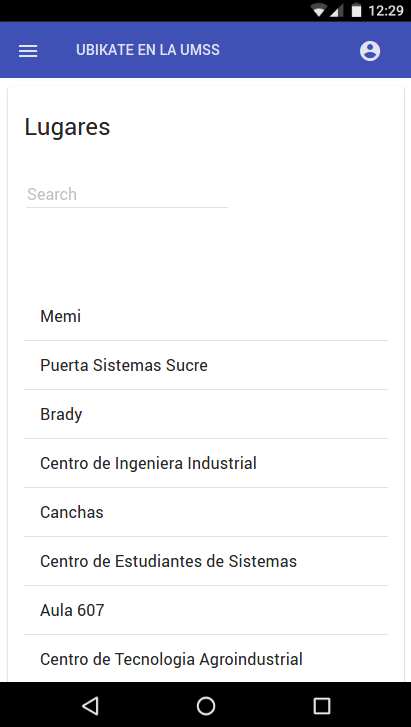
\includegraphics[width=0.3\textwidth]{iteration1/places_index_2}
    \caption{Lista de Lugares}
    \label{fig:places_index}
    \caption*{Fuente: Elaboración propia}
  \end{center}
\end{figure}


\subsubsection{Busqueda de los lugares}
\label{subs:busqueda de los lugares}

Para la implementacion de la busqueda de los lugares, un de los criterios de aceptacion es que sea posible la busqueda usando el nombre del lugar o parte del mismo, es necesario anadir un \emph{URI} adicional a nuestro servicio web, que obtenga de la base de datos un conjunto de lugares que concuerden con el criterio de busqueda, a continuacion se puede ver el URI implementado en la servicio web. \\

\begin{center}
  \begin{lstlisting}[label=endpoint_search_place,caption=Implementacion de la busqueda de lugares en el Servicio Web]

    router.get('places/search/:name', places.getPlacesByName);

  \end{lstlisting}
\end{center}


\subsubsection{Mostrar informacion del lugar}
\label{subs:Mostrar informacion del lugar}

La obtencion de la informacion de un lugar corresponde al URI \emph{places/:id} usando el verbo HTTP \emph{GET}, el cual obtiene la informacion en formato JSON, entonces se necesita mostrar esta informacion en el navegador, para lo cual el template correspondente al URI llegaria a ser \emph{templates/places/show}.

\begin{center}
  \begin{lstlisting}[label=template_places_show,caption=Template para mostrar la informacion de un lugar]
      {{#text.headline}}{{model.name}}{{/text.headline}}
      {{#card.content}}
          {{#paper-list}}
              {{model.description}}
              {{/paper-item}}
                  {{paper-icon "local_phone"}} {{model.phone}}
              {{/paper-item}}
              {{#paper-item class="md-2-line" }}
                  {{paper-icon "layers"}} Piso N# {{model.level}}
              {{/paper-item}}
          {{/paper-list}}
      {{/card.content}}

  \end{lstlisting}
\end{center}

El resultado del template renderizado en el navegador se puede apreciar en la figura \ref{fig:place_show}.

\begin{figure}[H]
  \begin{center}
    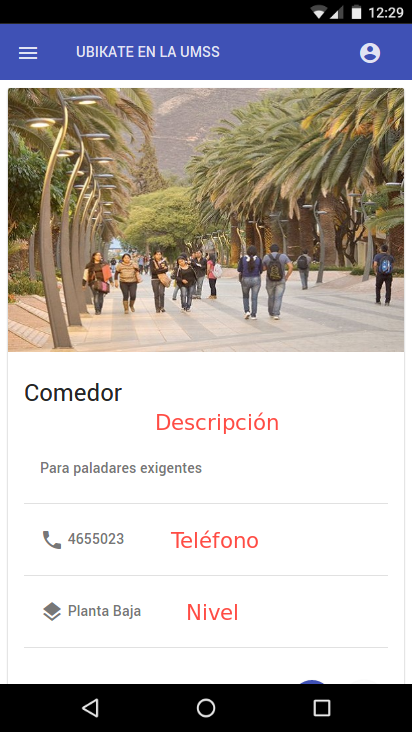
\includegraphics[width=0.3\textwidth]{iteration1/place_show}
    \caption{Vista de la Información de un Lugar.}
    \label{fig:place_show}
    \caption*{Fuente: Elaboración propia}
  \end{center}
\end{figure}




% En la figura \ref{fig:places_index}, se puede observar un


\subsection{Pruebas de Aceptación}

\begin{table}[H]
  \begin{center}
    \begin{tabularx}{0.75\textwidth}{ X }
      \toprule
      \textbf{Codigo:} CP001
      \makebox[3cm][r]{}
      \makebox[6cm][r]{\textbf{Historia de Usuario:} US01} \\

      \addlinespace
      \textbf{Nombre:} Verificar la lista de lugares. \\

      \addlinespace
      \textbf{Descripción:} Validar que un usuario visitante puede ver la lista de lugares cuando ingresa al menú \emph{lugares}. \\

      \addlinespace
      \textbf{Condiciones de Ejecución:} \\
      \tab \textbf{a.} El usuario no debe estar registrado. \\
      \tab \textbf{b.} Deben existir lugares registrados en el sistema.\\

      \addlinespace
      \textbf{Entradas / Pasos de Ejecución:}  \\
      \tab \textbf{1.} Hacer tap sobre el botón \emph{menú} en la esquina superior-izquierda. \\
      \tab \textbf{2.} Seleccionar el menú \emph{lugares}.\\

      \addlinespace
      \textbf{Resultado Esperado:} El Usuario debe ver una lista con los lugares registrados en la Condición de Ejecución \emph{b}.  \\

      \addlinespace
      \textbf{Evaluación de la Prueba:} Prueba exitosa. \\

      \bottomrule
    \end{tabularx}
    \caption{Prueba de Aceptación - CP001}
    \label{tab:CP001}
  \end{center}
\end{table}

\begin{table}[H]
  \begin{center}
    \begin{tabularx}{0.75\textwidth}{ X }
      \toprule
      \textbf{Codigo:} CP002
      \makebox[3cm][r]{}
      \makebox[6cm][r]{\textbf{Historia de Usuario:} US01} \\

      \addlinespace
      \textbf{Nombre:} Verificar la busqueda de lugares. \\

      \addlinespace
      \textbf{Descripción:} Validar que un usuario puede filtrar un lugar de la lista mediante el nombre. \\

      \addlinespace
      \textbf{Condiciones de Ejecución:} Ingresar en la base de datos el lugar con nombre ``MEMI''. \\

      \addlinespace
      \textbf{Entradas / Pasos de Ejecución:}  \\
      \tab \textbf{1.} Hacer tap sobre el botón \emph{menú} en la esquina superior-izquierda. \\
      \tab \textbf{2.} Seleccionar el menú \emph{lugares}.\\
      \tab \textbf{3.} Ingresar el nombre ``MEMI'' en el cajón de búsqueda.\\


      \addlinespace
      \textbf{Resultado Esperado:} Se debe mostrar un solo item en la lista de lugares con el nombre ``MEMI'' desplegado.\\

      \addlinespace
      \textbf{Evaluación de la Prueba:} Prueba exitosa. \\

      \bottomrule
    \end{tabularx}
    \caption{Prueba de Aceptación - CP002}
    \label{tab:CP002}
  \end{center}
\end{table}

\begin{table}[H]
  \begin{center}
    \begin{tabularx}{0.75\textwidth}{ X }
      \toprule
      \textbf{Codigo:} CP003
      \makebox[3cm][r]{}
      \makebox[6cm][r]{\textbf{Historia de Usuario:} US02} \\

      \addlinespace
      \textbf{Nombre:} Verificar la información de un lugar. \\

      \addlinespace
      \textbf{Descripción:} Validar que un usuario puede ver la descripción, el teléfono, el nivel y la foto de un lugar. \\

      \addlinespace
      \textbf{Condiciones de Ejecución:} Ingresar en la base de datos el lugar con nombre ``MEMI'' con su información completa. \\

      \addlinespace
      \textbf{Entradas / Pasos de Ejecución:}  \\
      \tab \textbf{1.} Hacer tap sobre el botón \emph{menú} en la esquina superior-izquierda. \\
      \tab \textbf{2.} Seleccionar el menú \emph{lugares}.\\
      \tab \textbf{3.} En la lista de lugares seleccionar el item ``MEMI''.\\

      \addlinespace
      \textbf{Resultado Esperado:} Se debe mostrar una pantalla con la foto del lugar ``MEMI'', su descripción, el teléfono y el nivel.\\

      \addlinespace
      \textbf{Evaluación de la Prueba:} Prueba exitosa. \\

      \bottomrule
    \end{tabularx}
    \caption{Prueba de Aceptación - CP003}
    \label{tab:CP003}
  \end{center}
\end{table}



\subsubsection{Resultado de las pruebas de la Iteración 1}

Al finalizar la Iteración 1, se ejecutaron todas las pruebas escritas durante la presente iteración, en el cuadro \ref{tab:regresion_1} se puede ver el detalle.


\begin{table}[H]
  \begin{center}
    \begin{tabularx}{0.8\textwidth}{ c  X  c }
      \toprule
        \textbf{Código} &
        \multicolumn{1}{c}{\textbf{Título de la Prueba}} &
        \textbf{Resultado}\\

      \midrule
        CP001
        &
        Verificar la lista de lugares.
        &
        Exitoso \\

\addlinespace
CP002
&
Verificar la busqueda de lugares.
&
Exitoso \\

\addlinespace
CP003
&
Verificar la información de un lugar.
&
Exitoso \\

\addlinespace
CP004
&
Verificar la lista de lugares cuando se busca un lugar no registrado.
&
Exitoso \\

\addlinespace
CP005
&
Verificar la información de un lugar mediante el URI.
&
Exitoso \\

\addlinespace
CP006
&
Verificar que el \emph{Menú} sea desplegado dinámicamente.
&
Exitoso \\



      \bottomrule
    \end{tabularx}
    \caption{Pruebas de regresión de la Iteración 1}
    \label{tab:regresion_1}
  \end{center}
\end{table}


\begin{itemize}
  \item Se ejecutaron 5 pruebas de funcionalidad, todas pasaron exitosamente.
  \item Se ejecutó 1 prueba de usabilidad, pasó exitosamente.
\end{itemize}


\section{Iteración 2}
\label{sec:iteracion_2}

Después de que finalizó la primera iteración y ya que todas las pruebas pasaron exitosamente, se continúa con la segunda iteración.


\subsection{Iteration Planning Meeting}
\label{sub:iteration2_planning_meeting}


Al igual que la primera iteración, las fases de exploración y planeación se realizan al mismo tiempo, en el sentido que no es necesario repartir las tareas resultantes de la exploración, por lo tanto al mismo tiempo en que se determinan las tareas se puede realizar la estimación de las mismas.

  \subsubsection{Exploración y Planeación}
  \label{subs:iteration2_exploracion_planeacion}

  Para la segunda iteración se toman en cuenta todas las historias de usuario restantes, y de acuerdo al criterio de escoger las siguientes historias más relevantes y de mayor valor para el producto, se escogió la historia de usuario #4.\\

  Como parte de la fase de Exploración se toma la historia de usuario #4 y la dividimos en las Tareas de Ingeniería, las cuales serán trabajadas en la fase de la Implementación.

  En la siguente tabla se especificaran las tareas correspondientes a la historia de usuario #4 \ref{tab:us04_tasks}. \\

  \subsection{Tareas del US04}
  \label{sub:us04_tasks}

    \begin{table}[H]
  \begin{center}
    \begin{tabularx}{\textwidth}{ c  X  C{2.3cm} }
      \toprule
        \textbf{Código} &
        \multicolumn{1}{c}{\textbf{Tarea}} &
        \textbf{Estimación [dias]}\\

      \midrule
        T011
        &
        Crear un archivo shapefile con información inicial de lugares principales dentro el campus de la UMSS.
        &
        2 \\

      \addlinespace
        T012
        &
        Preparar la base de datos para manejar información geográfica de rutas.
        &
        1 \\
      %
      % \addlinespace
      %   T013
      %   &
      %   Investigar e instalar una herramienta que permita usar un servicio de mapas.
      %   &
      %   1 \\

      % \addlinespace
      %   T014
      %   &
      %   El usuario puede ver un mapa usando un servicio del campus de la UMSS.
      %   &
      %   0.5 \\

      % \addlinespace
      %   T015
      %   &
      %   El usuario puede ver un marcador sobre el lugar.
      %   &
      %   0.5 \\
      %
      % \addlinespace
      %   T016
      %   &
      %   El marcador tiene información básica del lugar, nombre, piso.
      %   &
      %   0.5 \\

      \addlinespace
        T017
        &
        El usuario puede ver un marcador mostrando el lugar actual donde se encuentra (el usuario).
        &
        0.5 \\

      \addlinespace
        T018
        &
        Desarrollar un módulo que encuentra la ruta más corta usando la base de datos con información geográfica ruteable de T012.
        &
        2 \\

      \addlinespace
        T019
        &
        El usuario puede ver una línea roja que une el marcador de la posición del usuario con el marcador del lugar.
        &
        1 \\

      % \addlinespace
      %   TS003
      %   &
      %   Crear pruebas de funcionalidad del US04.
      %   &
      %   1 \\

      \addlinespace
      \midrule
        & \multicolumn{1}{R{7cm}}{\textbf{Total: }}
        & 10 \\

      \bottomrule
    \end{tabularx}
    \caption{Tareas del US04}
    \label{tab:us04_tasks}
  \end{center}
\end{table}


  \subsection{Calendario de Entregas}
  \label{subs:schedule_2}

    % \begin{table}[!ht]
%
% \end{table}
\begin{table}[H]

  \begin{center}

\begin{ganttchart}[
  canvas/.append style={fill=none, draw=black!5, line width=.75pt},
  hgrid style/.style={draw=black!5, line width=.75pt},
  vgrid={*1{draw=black!5, line width=.75pt}},
  %today=0,
  % today label=Semana 3,
  today rule/.style={
    draw=black!64,
    dash pattern=on 3.5pt off 4.5pt,
    line width=1.5pt
  },
  today label font=\small\bfseries,
  title/.style={draw=none, fill=none},
  title label font=\bfseries\footnotesize,
  title label node/.append style={below=7pt},
  include title in canvas=false,
  bar label font=\mdseries\small\color{black!70},
  bar label node/.append style={left=2cm},
  bar/.append style={draw=none, fill=black!63},
  bar incomplete/.append style={fill=barblue},
  bar progress label font=\mdseries\footnotesize\color{black!70},
  group incomplete/.append style={fill=groupblue},
    group left shift=0,
    group right shift=0,
    group height=.5,
    group peaks tip position=0,
    group label node/.append style={left=.6cm},
    group progress label font=\bfseries\small,
    link/.style={-latex, line width=1.5pt, linkred},
    link label font=\scriptsize\bfseries,
    link label node/.append style={below left=-2pt and 0pt},
  ]{1}{12}
  \gantttitle{Calendario de Entregasde de la Iteración 2}{7} \\[grid]
  \gantttitle{Semana 1}{7}
  \gantttitle{Semana 2}{7} \\
  % \gantttitle{Noviembre}{4} \\
  \gantttitle[title label node/.append style={below left=7pt and -3pt}]{D\'ia:\quad15}{0}
  \gantttitlelist{16,...,30}{1} \\
  % \ganttgroup[progress=0]{Historias de Usuario}{1}{8} \\
  \ganttbar[
    progress=0,
    name=bar1
  ]{\textbf{User Story 04}}{1}{12} \\
  % \ganttbar[
  %   progress=0,
  %   name=bar2
  % ]{\textbf{User Story 03}}{10}{12} \\
  % \ganttbar[
  %   progress=0,
  %   name=bar3
  % ]{\textbf{Iteración 3}}{5}{6} \\
  % \ganttbar[
  %   progress=0,
  %   name=bar4
  % ]{\textbf{Iteración 4}}{7}{8} \\
  % \ganttbar[
  %   progress=100,
  %   name=bar5
  % ]{\textbf{Actividad 5}}{5}{7} \\
  % \ganttbar[
  %   progress=80,
  % ]{\textbf{Actividad 6}}{8}{8} \\
  % \ganttbar[
  %   progress=49,
  % ]{\textbf{Actividad 7}}{9}{11} \\
  % \ganttmilestone{Hito 1}{11}{11}  \\
  % \ganttmilestone{Hito 2}{12}{12} \\
  %

  % \ganttmilestone{Q6 report}{24}{24} \\
  % \ganttmilestone{M1: Project finished}{8}{8}

  % \ganttlink[link type=f-s]{bar1}{bar2}
  % \ganttlink[link type=f-s]{bar2}{bar3}
  % \ganttlink[link type=f-s]{bar3}{bar4}

\end{ganttchart}

\caption{Calendario de Entregas de la Iteración 2}
\label{tab:calendario_entregas_iteracion_2}

\end{center}
\end{table}



\subsection{Implementación}
\label{sub:implementacion_iteracion_1}

Durante esta fase es donde se implementaran las tareas especificadas en la tabla \ref{tab:us04_tasks}.

\subsubsection{RF011}
\label{subs:RF011}

% Crear un archivo shapefile con la información geográfica de las rutas internas del campus de la UMSS

% Como ya se explico en \ref{sec:ruta_corta_umss}, esta tarea se llevo a cabo recabando la informacion geoespacial con un dispositivo GPS y exportando los datos resultantes a un archivo shapefile, el cual se puede apreciar en \ref{fig:shapefile_umss_v1}.

\subsubsection{RF012}
\label{subs:RF012}

% Preparar la base de datos para manejar información geográfica de rutas

% Para realizar esta tarea se procedió a instalar pgRouting, el resultado de esta tarea se puede apreciar en el manual de instalación ## \\
%
% Una vez configurada la base de datos se procede a cargar la misma con la informacion obtenida en RF011, para tal efecto es necesario primeramente crear una tabla que contendra los LINESTRING contenidos en el shapefile, esta operacion es similar a la realizada en la tarea - RF003 (\ref{sub:RF003}). Una vez que ya se tiene la tabla a la llamamos \emph{ways}, se necesita ejecutar un query propio de \emph{pgRouting} el cual tiene como objetivo analizar los datos geo-espaciales de la tabla y a\~nadirle una \emph{topologia}.
%
% Dentro lo que es la \emph{topologia geoespacial} existe una aplicacion que se lo conoce como \emph{topología de red}. La \emph{topología de red} representa las relaciones entre segmentos en una red lineal o una colección de segmentos de línea\cite{osgeo_journal_topology}.
% En un \emph{SIG} la topologia ayuda a mejorar el analisis de datos geo-espaciales, para resolver el problema de la ruta corta \emph{pgRouting} genera una \emph{topología de red} usando los datos que existen en la tabla \emph{ways}, es necesario ejecutar una instruccion, la que se muestra a continiacion y \emph{pgRouting} se encarga de llenar los datos que se pueden observar en la figura \ref{fig:postgres_ways}, las columnas \emph{source} y \emph{target} son populadas con el analisis topologico y en la figura \ref{fig:postgres_vertices}, se puede observar que la tabla \emph{ways\_vertices\_pgr} es creada enteramente en la ejecucion de la instruccion.
%
% \begin{verbatim}
%   select pgr_createTopology('ways', 0.00000001, 'geom', 'gid');
% \end{verbatim}
%
% \begin{figure}[H]
%   \begin{center}
%     \caption{Vista de la tabla \emph{ways} en la base de datos PostgreSQL.}
%     \label{fig:postgres_ways}
%     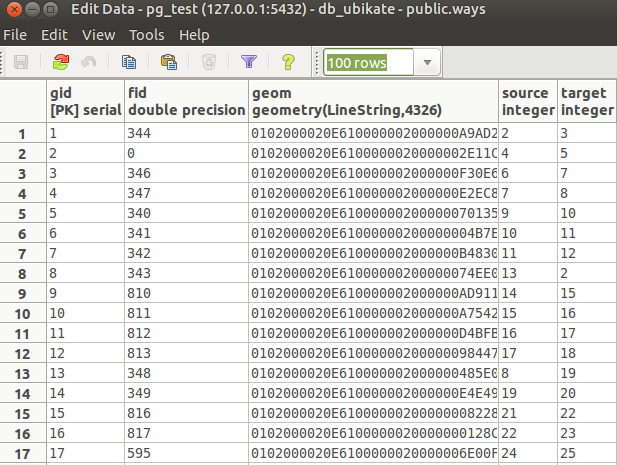
\includegraphics[width=1\textwidth]{iteration2/postgres_ways}
%     \caption*{Fuente: Elaboración propia}
%   \end{center}
% \end{figure}
%
% En la figura \ref{fig:postgres_ways} se puede apreciar que cada fila es una parte de la línea original obtenida por el dispositivo GPS y explisionada por QGIS, hay que notar que las columnas \emph{source} y \emph{target} hacen referencia a los nodos o vertices que la primera linea tiene en sus extremos, la primera linea o fila esta identificada por la columna \emph{gid}.\\
%
% En la siguiente figura \ref{fig:postgres_vertices} se observa la tabla \emph{ways\_vertices\_pgr} que contiene los vertices creados a partir del analisis de los datos en la tabla \emph{ways}.
%
% \begin{figure}[H]
%   \begin{center}
%     \caption{Vista de la tabla \emph{ways\_vertices\_pgr} en la base de datos PostgreSQL.}
%     \label{fig:postgres_vertices}
%     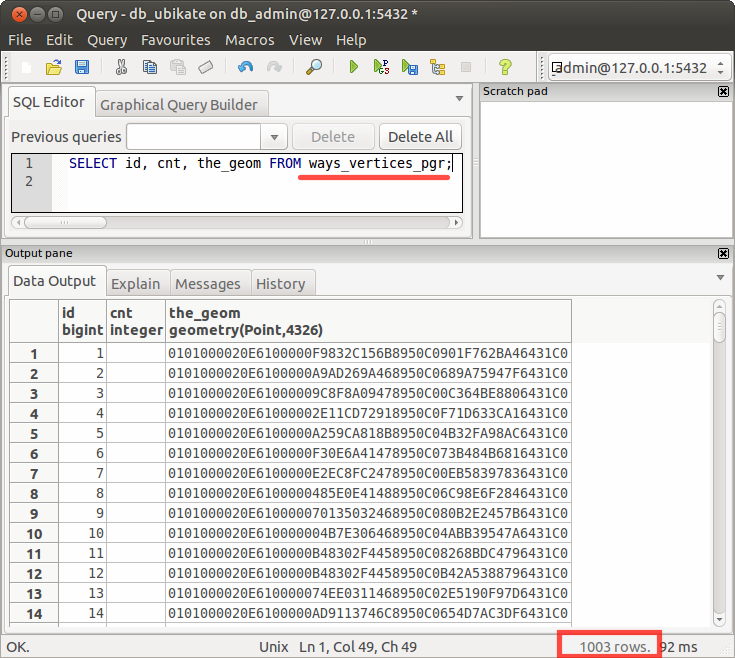
\includegraphics[width=1\textwidth]{iteration2/postgres_vertices}
%     \caption*{Fuente: Elaboración propia}
%   \end{center}
% \end{figure}
%
% Para entender los datos generados hay leer la informacion de las 2 tablas, por ejemplo en la primera  fila (gid 1) de la tabla \emph{ways}, se observa que el contenido de la columna \emph{source} es igual a \textbf{2} y \emph{target} es igual a \textbf{3}, eso quiere decir que los vertices del LINESTRING de la fila 1 son los vertices con \textbf{id} 2 y 3 respectivamente de la tabla \emph{ways\_vertices\_pgr}.\\
%
%
% Todo el conjunto de vertices y lineas de estas tablas se podria representar con una Matriz de adyacencias, explicada en \ref{sub:representacion_de_un_grafo}, y usada en la resolucion de la ruta mas corta, mas especificamente con el algoritmo de Dijkstra.

\subsubsection{RF013}
\label{subs:RF013}

% Investigar e instalar una herramienta que permita usar un servicio de mapas
% Durante la investigacion de esta tarea se encontro \emph{ember-leaflet}, una libreria o plugin que contiene las herramientas para poder cargar y usar un servicio de mapas.\\
%
% Para instalar esta libreria solo se necesita ejecutar el siguiente comando y posteriormente ya se puede empezar a utilizarla.\\
%
% \begin{verbatim}
%   $ ember install ember-leaflet
% \end{verbatim}
%
% El resultado de la investigacion puede apreciar en el marco teórico, en la sección que describe la librería, \emph{ember-leaflet}. \ref{sec:ember_js}

\subsubsection{RF014}
\label{subs:RF014}

% El usuario puede ver un mapa usando un servicio del campus de la UMSS

% Para completar esta tarea se hizo uso de la herramienta \emph{ember-leaflet}, con la cual se puede desplegar un mapa en el browser y optimizada para dispositivos moviles.\\
%
% \begin{verbatim}
%   {{#leaflet-map lat=lat lng=lng zoom=zoom}}
%     {{tile-layer
%       url="http://{s}.tile.openstreetmap.fr/hot/{z}/{x}/{y}.png"
%     }}
%   {{/leaflet-map}}
% \end{verbatim}
%
% Con la anterior instrucción se accede al servicio de \emph{Open Street Maps}, de la cual obtenemos los datos necesarios para renderizar un mapa en el browser. Los atributos de \emph{lat} y \emph{lng} se acceden de la capa del controlador de la aplicacion, son la latitud y longitud respectivamente, la convinacion de ambos datos es la locacion donde se va a ubicar el renderizado del mapa.\\

% Esta librería es la nos ayudará a insertar fácilmente los marcadores que irán sobre los lugares o la líneas que mostraran la ruta más corta
%
% Como resultado de esta tarea se puede apreciar la siguiente figura,

\subsubsection{RF015}
\label{subs:RF015}
% El usuario puede ver un marcador sobre el lugar

% Para completar esta tarea se continuó usando la librería \emph{ember-leaflet}, la cual permite que con la siguiente instrucción se despliegue un marcador sobre el mapa renderizado del API de \emph{Open Street Maps}.
%
% \begin{verbatim}
%   {{#marker-layer location=userLocation}} {{/marker-layer}}
% \end{verbatim}
%
% El resultado de la tarea se puede observar en la figura \ref{fig:baquita_place}.

\subsubsection{RF016}
\label{subs:RF016}
% marcador se  tiene información básica del lugar, nombre, piso

% Para poder mostrar la informacion del lugar sobre el marcador creado en RF015 se hizo uso de la librería \emph{ember-leaflet}, al igual que dicha tarea, solo se necesito de una instruccion para poder desplegar la informacion necesaria.
%
% \begin{verbatim}
%   {{#marker-layer location=location}}
%     h3>{{model.name}}</h3>
%     {{model.description}}
%     <strong>telf:</strong> {{model.phone}}
%     <strong>piso#</strong> {{model.level}}
%   {{/marker-layer}}
% \end{verbatim}
%
% En la figura \ref{fig:baquita_place} se puede apreciar el marcador con la información desplegada del lugar ``Baquita''.
%
% \begin{figure}[H]
%   \begin{center}
%     \caption{Tooltip con la información de un lugar.}
%     \label{fig:baquita_place}
%     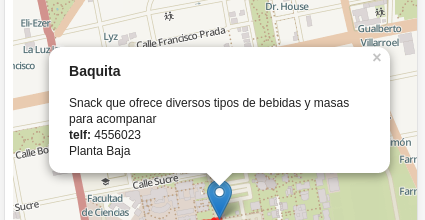
\includegraphics[width=1\textwidth]{iteration2/baquita_place}
%     \caption*{Fuente: Elaboración propia.}
%   \end{center}
% \end{figure}


\subsubsection{RF017}
\label{subs:RF017}
% El usuario puede ver un marcador mostrando el lugar actual donde se encuentra (el usuario)

% Para encontrar la locación del usuario se uso el API de geolocalización propio de HTML5, que en un smarthphone puede acceder y usar los recursos nativos de un smartphone, es necesaria la aceptacion del usuario mediante un mensaje que el navegador desplega, la locacion es encontrada mediante la triangulacion de Coordenadas por GPS (el mas exacto a la hora de encontrar la locacion del dispositvo), Wi-Fi, GSM o CDMA. Solo es necesaria la ejecucion de la siguente linea para ponder obetener la posición actual del usuario usando el API de geolocalización de HTML5.
%
% \begin{verbatim}
%   var coords = Geolocation.getCurrentPosition();
%   var latitud = coords.latitude;
%   var longitud = coords.longitude;
% \end{verbatim}
%
% La \emph{latitud} y \emph{longitud} obtenidas es fácilmente trasladado al mapa usando \emph{ember-leaflet} mediante un marcador, como se puede apreciar en la siguiente figura.
%
% \begin{figure}[H]
%   \begin{center}
%     \caption{Tooltip con la latitud y longitud de la posición actual del usuario.}
%     \label{fig:location_marker}
%     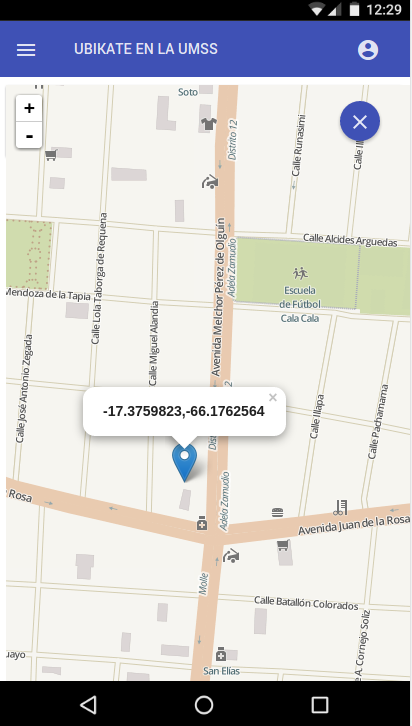
\includegraphics[width=0.5\textwidth]{iteration2/location_marker}
%     \caption*{Fuente: Elaboración propia.}
%   \end{center}
% \end{figure}

\subsubsection{RF018}
\label{subs:RF018}
% Desarrollar un módulo que encuentra la ruta más corta usando la base de datos con información geográfica ruteable de RF012

% Durante esta tarea se investigó la mejor forma de encontrar la ruta más corta y se llegó a la conclusión de usar la combinación de \emph{Postgres + Postgis + pgRouting}, esta investigación se puede apreciar en el marco teórico.\\
%
% Para hallar la ruta más corta se necesita usar las características de la base de datos para poder analizar los datos geográficos almacenados en la Tarea RF012, como el análisis que se requiere hacer es caro osea el costo de procesador para realizar los calculos necesarios es elevado, lo mas recomendable es que este trabajo sea realizado en el backend de la aplicacion por la base de datos.\\
%
% Tambien hay que tomar en cuenta que la tierra no es plana y las líneas que en un mapa parecen lineas rectas, realmente no son rectas, ya que el planeta Tierra es un \emph{esferoide oblato}\footnote{Un \emph{esferoide oblato} (o elipsoide oblato) es un elipsoide de revolución obtenido por rotación de una elipse alrededor de su eje más corto.} por lo que las lineas en apariencia rectas tienen la curvatura natural del planeta Tierra. En distancias largas esto tiene un gran impacto al manejar o utilizar mapas projectados, pero tambien es cierto que para una área pequeña como es el campus de la Universidad de San Simón este problema no tiene un gran impacto pero no está demás en tomar en cuenta esta característica del análisis de datos geoespaciales, como se explico en el capitulo \ref{cha:geolocalizacion}, para el presente proyecto se usara el proyeccion \emph{SRID 3857}.\\

% Una vez que se tienen en cuanta estas variables es necesaria la resolucion del problema de la ruta más corta, \emph{pgRouting} tiene varios métodos implementados para el analisis de datos geo-espaciales en la resolucion de este problema, para el presente proyecto se usara el algoritmo de \emph{Dijkstra}, explicado en el capítulo \ref{cha:ruta_optima}.\\
%
% Tomando en cuenta los conceptos aprendidos y las herramientas investigadas es que se desarrollo el modulo que encuentra la ruta mas corta.

% La siguiente SQL query está diseñado y explicado en la documentación de pgRouting {ref - link}, básicamente se necesita especificar el nodo inicio y el nodo destino y la base de datos se encarga de analizar la tabla creada en RF012, para que el algoritmo de Dijkstra funcione hay que darle un Costo a cada uno de los tramos pertenecientes a la Matriz, en este caso el costo será la longitud del tramo(st_length(geom) AS cost),  el costo de ir del punto A al punto B puede no ser la misma que de ir del punto B al punto A a pesar de ser una única línea, por ejemplo si la circulación fuera en un solo sentido  como en el caso de las rutas para automoviles, en este caso como es una ruta peatonal se simplifica un poco el problema, entonces como datos de entrada tenemos el punto donde se encuentra el usuario extraído por RF017 y el punto del lugar buscado extraído por RF0##, tomando en cuenta estos datos se armó el siguiente query,

% var raw = "SELECT seq, id1 AS node, id2 AS edge, cost " +
%             "FROM pgr_dijkstra('SELECT gid AS id, source::integer, target::integer, st_length(geom) AS cost " +
%             "                   FROM public.ways', " + targetId + ", " + sourceId + ", false, false);";

\subsubsection{RF019}
\label{subs:RF019}
% El usuario puede ver una línea roja que une el marcador de la posición del usuario con el marcador del lugar
% Como resultado de la tarea RF018 se tiene un conjunto de datos en formato de latitud y longitud que conforman líneas, las cuales representan la ruta más corta, pero al final es solo un montón de números, útiles pero para el usuario esta información es difícil de procesar, el usuario necesita información que sea fácil de entender y no existe mejor herramienta disponible para esta tarea que mostrar la \emph{ruta} de forma visual, esto quiere decir que se necesita mostrar la ruta sobre un \emph{mapa}, en la aplicación se usará \emph{ember-leaflet} para desplegar el mapa ofrecido por los servicios de OpenStreetMaps y también para mostrar ruta más corta mediante una línea de color rojo.\\
%
% Para resolver esta tarea se creó un servicio API usando ExpressJS, la cual se encarga obtener la información extraída de la base de datos y transformarla en un objeto JSON (GeoJSON), este objeto contiene la información geoespacial necesaria para ``dibujar'' la línea roja entre 2 puntos georeferenciados, uno de los cuales es el lugar al que se quiere llegar y el otro es la ubicación actual del usuario. \\
%
% \begin{verbatim}
%   ENV.APP.API_HOST + '/api/v1/ways/route/' + sourceData.id + '/' + targetData.id;
%
%   GET /api/v1/ways/route/930/77 200 276.217 ms - 3911
%
%   $ curl http://localhost:3000/api/v1/ways/route/930/77 | python -m json.tool                                                       [3:04:52]
%   % Total    % Received % Xferd  Average Speed   Time    Time     Time  Current
%                                  Dload  Upload   Total   Spent    Left  Speed
% 100  3911  100  3911    0     0   161k      0 --:--:-- --:--:-- --:--:--  166k
% {
%     "features": [
%         {
%             "geometry": {
%                 "coordinates": [
%                     [
%                         -66.1467397848201,
%                         -17.3935321732846
%                     ],
%                     [
%                         -66.1467190789842,
%                         -17.3935294725234
%                     ]
%                 ],
%                 "type": "LineString"
%             },
%             "type": "Feature"
%         },
%
% \end{verbatim}
% % /api/v1/ways/route/
%
% % Este objeto es representado en el mapa usando ember-leaflet con la siguiente instrucción,
% %
% % {{#geojson-layer geoJSON=currentGeoJSON color='red' }}
% % {{/geojson-layer}}
%
% Y se puede observar en el mapa una línea roja que representa la ruta más corta entre el punto donde se encuentra el usuario y el punto del lugar a buscar.
%
% \begin{figure}[H]
%   \begin{center}
%     \caption{Ruta más corta dibujada con una línea roja.}
%     \label{fig:short_way_place}
%     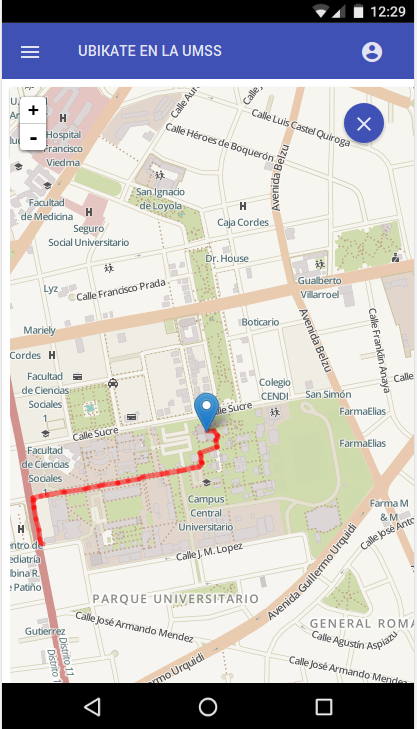
\includegraphics[width=0.5\textwidth]{iteration2/short_way_place}
%     \caption*{Fuente: Elaboración propia.}
%   \end{center}
% \end{figure}

\subsubsection{TS004}
\label{subs:TS004}

Pruebas funcionales

\subsection{Registrar el Avance}
\label{sub:iteracion2_avance}

\subsection{Verificación}
\label{sub:iteracion2_verificacion}

\section{Iteración 3}
\label{sec:iteracion_3}

% Al igual que al principio de la segunda iteración, se esperan los resultados de las pruebas realizadas para poder empezar con la planificación de la tercera iteración.

% \subsection{Iteration Planning Meeting}
% \label{sub:iteration2_planning_meeting}


% Los resultados de las pruebas realizadas se analizan para determinar si los criterios de aceptación, de las historias de usuario trabajadas en la segunda iteración, se cumplen para poder continuar con las historias que continúan sin ser desarrolladas, en caso que las pruebas fallen, es necesario continuar con la implementación de las historias inconclusas.\\
%
% En el caso del presente proyecto, las pruebas pasaron exitosamente y se aceptaron los criterios de aceptación de las historias de usuario trabajadas, por lo tanto se procede con la primera fase del “Iteration Planning”. \\

%
% \subsection{Exploración y Planeación}
% \label{sub:iteration2_exploracion_planeacion}

% Esta fase generalmente se realiza en 2 pasos pero será realizada al mismo tiempo, ya que en la exploración se definen las tareas a realizar y en la planeación se asigna estas tareas al equipo de desarrollo, el cual tiene que estimar las tareas, pero como el equipo de desarrollo está compuesto por mi persona, puedo definir las tareas y asignarles una estimación en el mismo paso.\\
%
% Para la Iteración 3, se trabajarán las historias de usuario 6 y 7, de las que a continuación se definirán sus tareas de ingeniería. \\


\subsection{Planificación de la Iteración 3}

  A continuación se analizará la \emph{historia de usuario} US06, ver el cuadro \ref{tab:US06}.

    
\begin{table}[H]
\begin{center}
  \begin{tabularx}{0.75\textwidth}{ X }
    \toprule
    \textbf{Historia de Usuario:} US06
    \makebox[6cm][r]{\textbf{Prioridad:} Alta} \\
    \makebox[4cm][r]{}
    \makebox[6cm][r]{\textbf{Riesgo:} Alto} \\

    \addlinespace
    \textbf{Nombre:} Añadir más lugares al sistema.\\

    \addlinespace
    \textbf{Descripción:} \\
    \tab Yo como usuario registrado.\\
    \tab Deseo añadir más lugares al sistema. \\
    \tab Para mejorar los criterios de busqueda. \\

    \addlinespace
    \textbf{Criterios de Aceptación:} \\
    \tab Quiero que sea posible anadir un lugar si no lo encuentro en la lista de lugares. \\
    \tab Quiero ver un formulario para poder ingresar los datos de un nuevo lugar.\\
    \tab Quiero pararme cerca o en el lugar que necesito añadir para georeferenciarlo. \\

    \bottomrule
  \end{tabularx}
  \caption{Historia de Usuario - US06}
  \label{tab:US06}
\end{center}
\end{table}


    \begin{table}[H]
  \begin{center}
    \begin{tabularx}{0.75\textwidth}{ X }
      \toprule
      \textbf{Número de Tarea:} T019
      \makebox[1cm][r]{}
      \makebox[6cm][r]{\textbf{Historia de Usuario:} US06} \\

      \addlinespace
      \textbf{Descripción:} Implementar en el backend el \emph{endpoint} para añadir y editar usuarios. \\

      \addlinespace
      \textbf{Tipo de Tarea:} Desarrollo
      \makebox[6cm][r]{\textbf{Estimación [dias]:} 1} \\

      \addlinespace
      \textbf{Programador Responsable:} Edmundo Figueroa \\

      \bottomrule
    \end{tabularx}
    \caption{Tarea de Ingeniería - T019}
    \label{tab:T019}
  \end{center}
\end{table}


\begin{table}[H]
  \begin{center}
    \begin{tabularx}{0.75\textwidth}{ X }
      \toprule
      \textbf{Número de Tarea:} T020
      \makebox[1cm][r]{}
      \makebox[6cm][r]{\textbf{Historia de Usuario:} US06} \\

      \addlinespace
      \textbf{Descripción:} Mostrar un botón para añadir lugares solamente a usuarios registrados. \\

      \addlinespace
      \textbf{Tipo de Tarea:} Desarrollo
      % \makebox[1cm][r]{}
      \makebox[6cm][r]{\textbf{Estimación [dias]:} 0.5} \\

      \addlinespace
      \textbf{Programador Responsable:} Edmundo Figueroa \\

      \bottomrule
    \end{tabularx}
    \caption{Tarea de Ingeniería - T020}
    \label{tab:T020}
  \end{center}
\end{table}

\begin{table}[H]
  \begin{center}
    \begin{tabularx}{0.75\textwidth}{ X }
      \toprule
      \textbf{Número de Tarea:} T021
      \makebox[1cm][r]{}
      \makebox[6cm][r]{\textbf{Historia de Usuario:} US06} \\

      \addlinespace
      \textbf{Descripción:} Mostrar un formulario para añadir más lugares, con el nombre del lugar, descripción, teléfono y nivel. \\

      \addlinespace
      \textbf{Tipo de Tarea:} Desarrollo
      \makebox[6cm][r]{\textbf{Estimación [dias]:} 0.5} \\

      \addlinespace
      \textbf{Programador Responsable:} Edmundo Figueroa \\

      \bottomrule
    \end{tabularx}
    \caption{Tarea de Ingeniería - T021}
    \label{tab:T021}
  \end{center}
\end{table}

\begin{table}[H]
  \begin{center}
    \begin{tabularx}{0.75\textwidth}{ X }
      \toprule
      \textbf{Número de Tarea:} T022
      \makebox[1cm][r]{}
      \makebox[6cm][r]{\textbf{Historia de Usuario:} US06} \\

      \addlinespace
      \textbf{Descripción:} Registrar las coordenadas del lugar al momento de crear un nuevo lugar. \\

      \addlinespace
      \textbf{Tipo de Tarea:} Desarrollo
      \makebox[6cm][r]{\textbf{Estimación [dias]:} 1} \\

      \addlinespace
      \textbf{Programador Responsable:} Edmundo Figueroa \\

      \bottomrule
    \end{tabularx}
    \caption{Tarea de Ingeniería - T022}
    \label{tab:T022}
  \end{center}
\end{table}


\begin{table}[H]
  \begin{center}
    \begin{tabularx}{0.75\textwidth}{ X }
      \toprule
      \textbf{Número de Tarea:} T023
      \makebox[1cm][r]{}
      \makebox[6cm][r]{\textbf{Historia de Usuario:} US06} \\

      \addlinespace
      \textbf{Descripción:} Implementar el modulo para poder agregar una foto a un lugar. \\

      \addlinespace
      \textbf{Tipo de Tarea:} Desarrollo
      \makebox[6cm][r]{\textbf{Estimación [dias]:} 1} \\

      \addlinespace
      \textbf{Programador Responsable:} Edmundo Figueroa \\

      \bottomrule
    \end{tabularx}
    \caption{Tarea de Ingeniería - T023}
    \label{tab:T023}
  \end{center}
\end{table}


  A continuación se analizará la \emph{historia de usuario} US07, ver el cuadro \ref{tab:US07}.

    
\begin{table}[H]
\begin{center}
 \begin{tabularx}{0.75\textwidth}{ X }
   \toprule
   \textbf{Historia de Usuario:} US07
   \makebox[6cm][r]{\textbf{Prioridad:} Alta} \\
   \makebox[4cm][r]{}
   \makebox[6cm][r]{\textbf{Riesgo:} Alto} \\

   \addlinespace
   \textbf{Nombre:} Editar la información de un lugar.\\

   \addlinespace
   \textbf{Descripción:} \\
   \tab Yo como usuario registrado.\\
   \tab Deseo editar la información de un lugar. \\
   \tab Para mejorar o corregir la información de ese lugar. \\

   \addlinespace
   \textbf{Criterios de Aceptación:} \\
   \tab Al entrar a la información de un lugar quiero ser el único que vea un icono para poder entrar a la edición de los datos. \\
   \tab Quiero acceder a un formulario que muestre la información actual del lugar y poder editar la información mostrada. \\

   \bottomrule
 \end{tabularx}
 \caption{Historia de Usuario - US07}
 \label{tab:US07}
\end{center}
\end{table}


    \begin{table}[H]
  \begin{center}
    \begin{tabularx}{0.75\textwidth}{ X }
      \toprule
      \textbf{Número de Tarea:} T024
      \makebox[1cm][r]{}
      \makebox[6cm][r]{\textbf{Historia de Usuario:} US07} \\

      \addlinespace
      \textbf{Descripción:} Implementar el modulo para editar lugares. \\

      \addlinespace
      \textbf{Tipo de Tarea:} Desarrollo
      \makebox[6cm][r]{\textbf{Estimación [dias]:} 1} \\

      \addlinespace
      \textbf{Programador Responsable:} Edmundo Figueroa \\

      \bottomrule
    \end{tabularx}
    \caption{Tarea de Ingeniería - T024}
    \label{tab:T024}
  \end{center}
\end{table}


\begin{table}[H]
  \begin{center}
    \begin{tabularx}{0.75\textwidth}{ X }
      \toprule
      \textbf{Número de Tarea:} T025
      \makebox[1cm][r]{}
      \makebox[6cm][r]{\textbf{Historia de Usuario:} US07} \\

      \addlinespace
      \textbf{Descripción:} Mostrar un botón para editar un lugar solamente a usuarios administradores. \\

      \addlinespace
      \textbf{Tipo de Tarea:} Desarrollo
      % \makebox[1cm][r]{}
      \makebox[6cm][r]{\textbf{Estimación [dias]:} 0.5} \\

      \addlinespace
      \textbf{Programador Responsable:} Edmundo Figueroa \\

      \bottomrule
    \end{tabularx}
    \caption{Tarea de Ingeniería - T025}
    \label{tab:T025}
  \end{center}
\end{table}

\begin{table}[H]
  \begin{center}
    \begin{tabularx}{0.75\textwidth}{ X }
      \toprule
      \textbf{Número de Tarea:} T026
      \makebox[1cm][r]{}
      \makebox[6cm][r]{\textbf{Historia de Usuario:} US07} \\

      \addlinespace
      \textbf{Descripción:} Mostrar la información actual del lugar en el formalario de edicion. \\

      \addlinespace
      \textbf{Tipo de Tarea:} Desarrollo
      \makebox[6cm][r]{\textbf{Estimación [dias]:} 0.5} \\

      \addlinespace
      \textbf{Programador Responsable:} Edmundo Figueroa \\

      \bottomrule
    \end{tabularx}
    \caption{Tarea de Ingeniería - T026}
    \label{tab:T026}
  \end{center}
\end{table}

\begin{table}[H]
  \begin{center}
    \begin{tabularx}{0.75\textwidth}{ X }
      \toprule
      \textbf{Número de Tarea:} T027
      \makebox[1cm][r]{}
      \makebox[6cm][r]{\textbf{Historia de Usuario:} US07} \\

      \addlinespace
      \textbf{Descripción:} Mostrar un boton para eliminar el lugar solamente a un usuario administrador. \\

      \addlinespace
      \textbf{Tipo de Tarea:} Desarrollo
      \makebox[6cm][r]{\textbf{Estimación [dias]:} 1} \\

      \addlinespace
      \textbf{Programador Responsable:} Edmundo Figueroa \\

      \bottomrule
    \end{tabularx}
    \caption{Tarea de Ingeniería - T027}
    \label{tab:T027}
  \end{center}
\end{table}



% \subsubsection{Tareas del US06}
% \label{sub:us06_tasks}

% \begin{table}[H]
  \begin{center}
    \begin{tabularx}{\textwidth}{ c  X  C{2.3cm} }
      \toprule
        \textbf{Código} &
        \multicolumn{1}{c}{\textbf{Tarea}} &
        \textbf{Estimación [dias]}\\

      \midrule
        T020
        &
        El usuario podrá ver un link hacia el formulario para añadir más lugares desde la lista de lugares existentes.
        &
        0.5 \\

      \addlinespace
        T021
        &
        El usuario podrá ver un formulario para añadir un lugar con información básica. por ejemplo, el nombre del lugar, descripción, teléfono.
        &
        1 \\

      \addlinespace
        T022
        &
        El usuario deberá estar cerca del lugar que desea añadir para poder georeferenciarlo.
        &
        1 \\

      \addlinespace
        T023
        &
        Un usuario no-administrador no debería poder ver el formulario para añadir lugares.
        &
        1 \\


      \addlinespace
        P004
        &
        Crear pruebas de funcionalidad del US05.
        &
        0.5 \\

      \addlinespace
      \midrule
        & \multicolumn{1}{R{7cm}}{\textbf{Total: }}
        & 4 \\

      \bottomrule
    \end{tabularx}
    \caption{Tareas del US05}
    \label{tab:us05_tasks}
  \end{center}
\end{table}

%
%
% \subsubsection{Tareas del US07}
% \label{sub:us07_tasks}

  % \begin{table}[H]
  \begin{center}
    \begin{tabularx}{\textwidth}{ c  X  C{2.3cm} }
      \toprule
        \textbf{Código} &
        \multicolumn{1}{c}{\textbf{Tarea}} &
        \textbf{Estimación [dias]}\\

      \midrule
      T024
      &
      Implementar en el backend el \emph{endpoint} para eliminar usuarios.
      &
      0.5 \\

      \addlinespace
        T024
        &
        Mostrar un boton solamente al administrador para editar un lugar.
        &
        0.5 \\

      \addlinespace
        T025
        &
        Mostrar la información actual del lugar en el formalario de edicion
        % El usuario debería poder ver la información actual del lugar en el formulario para editar el lugar.
        &
        1 \\

      \addlinespace
        T026
        &
        Mostrar un boton para eliminar el lugar solamente a un usuario administrador.
        % El usuario no-administrador no debería poder ver el link hacia el formulario para editar el lugar.
        &
        1 \\

      \addlinespace
        P005
        &
        Crear pruebas de funcionalidad del US06.
        &
        0.5 \\

      \addlinespace
      \midrule
        & \multicolumn{1}{R{7cm}}{\textbf{Total: }}
        & 3 \\

      \bottomrule
    \end{tabularx}
    \caption{Tareas del US06}
    \label{tab:us06_tasks}
  \end{center}
\end{table}



  % \subsection{Implementación}
  % \label{sub:implementacion_iteracion_3}

  \subsection{Implementación de la Iteración 3}


      
% \subsubsection{Implementar módulo para añadir lugares al sistema}
\subsubsection{Registro de Lugares en el sistema}

Para registrar un \emph{lugar} primeramente se implementó el formulario que se usará para recolectar la información del \emph{lugar}, el formulario fue creado usando \emph{EmberJs} y se lo puede ver en la figura \ref{fig:new_place}. \\

\begin{figure}[H]
     \begin{center}
       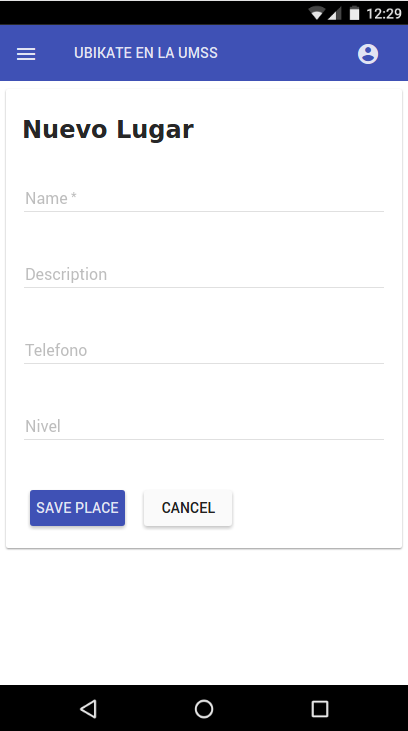
\includegraphics[width=0.3\textwidth]{new_place}

       \caption{Formulario para añadir un nuevo \emph{lugar}.}
       \label{fig:new_place}
       \caption*{Fuente: Elaboración propia.}
     \end{center}
\end{figure}

Posteriormente es necesario crear la petición HTTP desde el controlador de \emph{EmberJS} hacia el API, en el cuerpo de la petición se incluye la posición georeferenciada del celular utilizando el API de Geolocalización de HTML5 usada anteriormente para encontrar la ubicación del usuario, también se incluye el nombre, la descripción, el teléfono y el nivel del \emph{lugar}. En el codigo \ref{new_place_request} se puede ver la implementación de la petición.


% En la figura \ref{fig:new_place} se puede ver el formulario implementado usando \emph{ember-paper}, el cual colecciona los datos que se quieren introducir y se los envía al backend usando una llamada AJAX, como se puede ver en el siguiente código, para crear la petición POST se obtiene las coordenadas actuales del dispositivo móvil además de los datos recolectados del formulario y que con la ayuda de \emph{JQuery} es enviado al API el cual maneja la información recibida y se encarga de insertar los datos en la base de datos.\\

% \newpage
\begin{center}
 \begin{lstlisting}[label=new_place_request,caption=POST request creado en el controlador de \emph{ember}]

   var payload = {
       name: nombre,
       description: descripcion,
       phone: telefono,
       level: nivel,
       lat: latitud,
       lon: longitud
   };

   var url = (ENV.APP.API_HOST || '') + '/api/v1/places/';
   jQuery.post(url, payload).then(
       function(data) {
           var transition = controller.get('transition');
           if (transition) {
               self.transitionTo('places.show');
           } else {
               self.transitionTo('places');
           }
       },
       function(error) {
           controller.set('message', error.responseText);
       }
   );

 \end{lstlisting}
\end{center}

% En esta iteración se implementó la opción de añadir más lugares al sistema, de editarlos y eliminarlos, y la primera tarea es crear las consultas SQL para llevar a cabo las tareas. \\

% por lo que es necesario crear las consultas SQL que insertaran los datos enviados desde el dispositivo móvil al servidor. \\

% Como requisito para insertar un nuevo ``lugar'', se requiere que el usuario esté posicionado en el ``lugar'' ya que se usaran sus coordenadas para posicionar el ``lugar''. Las coordenadas del usuario son obtenidas usando el API de Geolocalización propia de HTML5, usada anteriormente para encontrar la ubicación del usuario \emph{visitante} en la iteración 2.\\

% Posteriormente se necesita implementar el formulario que el usuario usará para insertar los datos del ``lugar'': el nombre, la descripción, el teléfono y el nivel.\\

% Para insertar un ``lugar''  en la base de datos se usó el codigo \ref{new_place}, donde se puede observar la consulta SQL usada, para la cual se necesita capturar la latitud y longitud respectiva donde se encuentra el usuario, además de los datos del ``lugar''.\\

La petición creada es recibida en el API utilizando el \emph{endpoint} RESTful designado para ello, \verb|router.post('/', places.newPlace);|, el \emph{endpoint} se encarga de mandar la información recibida hacia la base de de datos, tomando en cuenta que la posición del lugar es un tipo especial de la base de datos, la latitud y longitud necesitan ser transformadas al momento de insertar el \emph{lugar} en la base de datos, como se muestra en el codigo \ref{cod-new_place_api}.


\begin{center}
 \begin{lstlisting}[label=cod-new_place_api,caption=Insertar un ``lugar'' en la base de datos.]

   router.post('/', places.newPlace);

   var newPlace = (req, res) => {
       var name = req.body.name || '';
       var lat = req.body.lat || '';
       var lon = req.body.lon || '';
       var description = req.body.description || '';
       var phone = req.body.phone || '';
       var level = req.body.level || '';

       let raw = `insert into place (name, geom, description, phone, level)
                  values ('${name}',
                          ST_GeomFromText('POINT(${lon} ${lat})', 3875),
                          '${description}',
                          '${phone}',
                          '${level}'
                         );`;

       Knex.raw(raw)
           .then(function(data) {
               res.json({
                   "message": "Place saved successfully!",
                   "data": data
               });
           })
           .catch(function(error) {
               res.send("Error:", error);
           });
   };

 \end{lstlisting}
\end{center}




% Para la creación de un ``lugar'' es necesario implementar un \emph{endpoint} en el API y siguiendo las convenciones REST se , para que como ya se explicó anteriormente el frontend pueda comunicarse con el backend. \\

% En el API de la aplicación, se implementó un \emph{endpoint} para que pueda manejar los \emph{request} del cliente para añadir un lugar, este \emph{request} es enviado usando el verbo HTTP \emph{POST}, que como ya se explicó es el usado en un REST API para crear objetos. \\

\subsubsection{Edición de la información del Lugar}

Para editar de la información de un lugar se rehusó el formulario ya creado para el registro del mismo, pero populando los campos con la información actual del lugar, el resultado se lo puede ver en la figura \ref{fig:place_edit_form}. \\

\begin{figure}[H]
     \begin{center}
       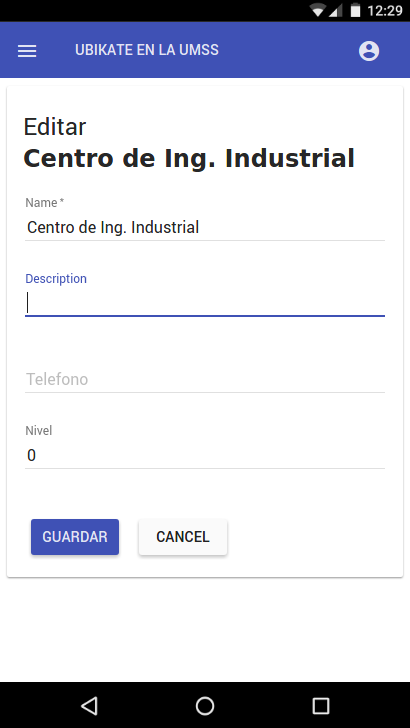
\includegraphics[width=0.3\textwidth]{place_edit_form}

       \caption{Formulario para editar un \emph{lugar}}
       \label{fig:place_edit_form}
       \caption*{Fuente: Elaboración propia.}
     \end{center}
\end{figure}


Los cambios a la información del \emph{lugar} son enviados al API mediante una petición PUT, siguiendo los lineamientos del REST API implementado, esta petición se puede ver en el codigo \ref{cod-edit_place_request}.

% \newpage
\begin{center}
 \begin{lstlisting}[label=cod-edit_place_request,caption=Petición HTTP para editar un lugar.]

   router.put('/:id', places.editPlace);

   var body = {
       name: name,
       description: description,
       phone: phone,
       level: level
   };

   var url = (ENV.APP.API_HOST || '') + `/api/v1/places/${id}`;
   jQuery.ajax({
       url: url,
       type: 'put',
       data: body
   }).then(
       function(data) {
           self.transitionTo('places.show', id);
       },
       function(error) {
           controller.set('message', error.responseText);
       }
   );

 \end{lstlisting}
\end{center}

A diferencia del registro del \emph{lugar}, que guarda la posición georeferenciada al momento de registrar el \emph{lugar}, en la edición de los datos no se está tomando en cuenta este dato porque se noto que generalmente cuando se requiere actualizar los datos del \emph{lugar}, el usuario no se encuentra en la posición original del \emph{lugar} y este dato se pierde, corrompiendo la base de datos. Es por esta razón que se decidió que no se actualizará la posición geográfica del \emph{lugar} sin alguna opción explícita que advierta al usuario de las consecuencias de esta acción, pero como tal tarea no se halla dentro de la \emph{historia de usuario} que se esta implementado, se tomo la decisión de realizarla en una futura iteración.








% \subsubsection{Eliminar un lugar}

% Una vez implementado la lógica para añadir un ``lugar'', se implementó los módulos para poder eliminar el ``lugar'', para esto se añadió un botón en la lista de lugares, el cual despliega un mensaje de advertencia al usuario de que está por eliminar un ``lugar'' y que la acción es irreversible, por lo tanto este botón sólo está disponible para un usuario \emph{administrador}. \\
%
% La verbo  HTTP \emph{DELETE} es el que de acuerdo a la implementación del API REST es el adecuado para eliminar un lugar, por lo tanto es el que se usó en la aplicación. En el codigo \ref{delete_place_enpoint} se puede observar el \emph{endpoint} implementado en el API que se encarga de manejar las peticiones \emph{DELETE} creando una consulta SQL que elimina el lugar de la base de datos.\\
%
% \begin{center}
%   \begin{lstlisting}[label=delete_place_enpoint,caption=DELETE request elimina un lugar.]
%
%     router.delete('/:id', places.deletePlace);
%
%     var deletePlace = (req, res) => {
%         var id = req.params.id;
%
%         Place.forge({
%             gid: id
%         })
%         .destroy()
%         .then(function(model) {
%             res.json({
%                 "message": "Place deleted successfully!"
%             });
%         })
%         .catch(function(err) {
%             res.status(500);
%         });
%     };
%
%   \end{lstlisting}
% \end{center}
%
% En el anterior codigo se puede apreciar la bondad de usar un manejador de bases de datos como \emph{Bookshelf} ya que usando el método \verb|destroy()|, se encarga automáticamente de crear la consulta SQL para eliminar una tupla de la base de datos.\\


  \subsection{Pruebas de Aceptación de la Iteración 3}

      \begin{table}[H]
  \begin{center}
    \begin{tabularx}{0.75\textwidth}{ X }
      \toprule
      \textbf{Codigo:} CP012
      \makebox[3cm][r]{}
      \makebox[6cm][r]{\textbf{Historia de Usuario:} US06} \\

      \addlinespace
      \textbf{Tipo:} Prueba de Funcionalidad - Positiva. \\

      \addlinespace
      \textbf{Nombre:} Verificar el registro de lugares. \\

      \addlinespace
      \textbf{Descripción:} Validar que un usuario registrado puede añadir un lugar nuevo al sistema. \\

      \addlinespace
      \textbf{Condiciones de Ejecución:} \\
      \tab \textbf{a.} El usuario debe estar registrado. \\
      % \tab \textbf{b.} Registrar un lugar dentro del campus Universitario.\\

      \addlinespace
      \textbf{Entradas / Pasos de Ejecución:}  \\
      \tab \textbf{1.} Seleccionar el menú \emph{Lugares}. \\
      \tab \textbf{2.} Hacer tap sobre el icono de registro de lugares.\\
      \tab \textbf{3.} Ingresar el Nombre del lugar.\\
      \tab \textbf{4.} Ingresar una Descripción del lugar.\\
      \tab \textbf{5.} Ingresar el Teléfono del lugar.\\
      \tab \textbf{6.} Ingresar el Nivel del lugar.\\
      \tab \textbf{7.} Aceptar el formulario.\\


      \addlinespace
      \textbf{Resultado Esperado:} Una vista de la información del lugar es desplegada con los datos ingresados en los pasos.  \\

      \addlinespace
      \textbf{Evaluación de la Prueba:} Prueba exitosa. \\

      \bottomrule
    \end{tabularx}
    \caption{Prueba de Aceptación - CP012}
    \label{tab:CP012}
  \end{center}
\end{table}

\begin{table}[H]
  \begin{center}
    \begin{tabularx}{0.75\textwidth}{ X }
      \toprule
      \textbf{Codigo:} CP013
      \makebox[3cm][r]{}
      \makebox[6cm][r]{\textbf{Historia de Usuario:} US07} \\

      \addlinespace
      \textbf{Tipo:} Prueba de Funcionalidad - Positiva. \\

      \addlinespace
      \textbf{Nombre:} Verificar la edición de la información de un lugar. \\

      \addlinespace
      \textbf{Descripción:} Validar que un usuario registrado puede editar la información de un lugar. \\

      \addlinespace
      \textbf{Condiciones de Ejecución:} \\
      \tab \textbf{a.} El usuario debe estar registrado. \\
      \tab \textbf{b.} Registrar un lugar dentro del campus Universitario.\\

      \addlinespace
      \textbf{Entradas / Pasos de Ejecución:}  \\
      \tab \textbf{1.} Seleccionar el menú \emph{Lugares}. \\
      \tab \textbf{2.} Buscar el lugar registrado en las condiciones.\\
      \tab \textbf{3.} Editar el Nombre del lugar.\\
      \tab \textbf{4.} Editar la Descripción del lugar.\\
      \tab \textbf{5.} Editar el Teléfono del lugar.\\
      \tab \textbf{6.} Editar el Nivel del lugar.\\
      \tab \textbf{7.} Aceptar el formulario.\\


      \addlinespace
      \textbf{Resultado Esperado:} Una vista de la información del lugar es desplegada con la información editada en los pasos.  \\

      \addlinespace
      \textbf{Evaluación de la Prueba:} Prueba exitosa. \\

      \bottomrule
    \end{tabularx}
    \caption{Prueba de Aceptación - CP013}
    \label{tab:CP013}
  \end{center}
\end{table}


\begin{table}[H]
  \begin{center}
    \begin{tabularx}{0.75\textwidth}{ X }
      \toprule
      \textbf{Codigo:} CP014
      \makebox[3cm][r]{}
      \makebox[6cm][r]{\textbf{Historia de Usuario:} US06} \\

      \addlinespace
      \textbf{Tipo:} Prueba de Funcionalidad - Negativa. \\

      \addlinespace
      \textbf{Nombre:} Verificar que no pueda registrar un lugar fuera del campus Universitario. \\

      \addlinespace
      \textbf{Descripción:} Validar que los lugares que están fuera del campus Universitario no pueda ser registrado en el sistema. \\

      \addlinespace
      \textbf{Condiciones de Ejecución:} \\
      \tab \textbf{a.} El usuario debe estar registrado. \\
      \tab \textbf{b.} El usuario debe estar fuera de los predios del Campus Universitario.\\

      \addlinespace
      \textbf{Entradas / Pasos de Ejecución:}  \\
      \tab \textbf{1.} Seleccionar el menú \emph{Lugares}. \\
      \tab \textbf{2.} Hacer tap sobre el icono de registro de lugares.\\

      \addlinespace
      \textbf{Resultado Esperado:} Un mensaje debería ser desplegado informando que no se pueden registrar Lugares fuera del Campus Universitario.  \\

      \addlinespace
      \textbf{Evaluación de la Prueba:} Prueba fallada. \\

      \bottomrule
    \end{tabularx}
    \caption{Prueba de Aceptación - CP014}
    \label{tab:CP014}
  \end{center}
\end{table}


\begin{table}[H]
  \begin{center}
    \begin{tabularx}{0.75\textwidth}{ X }
      \toprule
      \textbf{Codigo:} CP015
      \makebox[3cm][r]{}
      \makebox[6cm][r]{\textbf{Historia de Usuario:} US06, US07} \\

      \addlinespace
      \textbf{Tipo:} Prueba de Usabilidad. \\

      \addlinespace
      \textbf{Nombre:} Verificar los campos de texto de los formularios de registro y edición. \\

      \addlinespace
      \textbf{Descripción:} Validar que los campos de texto dentro los formularios de registro y edición de lugares no exceda la longitud de la pantalla del dispositivo móvil. \\

      \addlinespace
      \textbf{Condiciones de Ejecución:} \\
      \tab \textbf{a.} El usuario debe estar registrado. \\
      % \tab \textbf{b.} El usuario debe estar fuera de los predios del Campus Universitario.\\

      \addlinespace
      \textbf{Entradas / Pasos de Ejecución:}  \\
      \tab \textbf{1.} Seleccionar el menú \emph{Lugares}. \\
      \tab \textbf{2.} Presionar el icono de registro de lugares.\\
      \tab \textbf{3.} Insertar texto en los campos de descripción, teléfono y nombre.\\
      \tab \textbf{4.} Repetir para el formulario de edición de lugares.\\

      \addlinespace
      \textbf{Resultado Esperado:} El texto escrito no debería sobrepasar la longitud del dispositivo móvil en los formularios de registro y edición de lugares.  \\

      \addlinespace
      \textbf{Evaluación de la Prueba:} Prueba exitosa. \\

      \bottomrule
    \end{tabularx}
    \caption{Prueba de Aceptación - CP015}
    \label{tab:CP015}
  \end{center}
\end{table}


  % \subsection{Registrar el Avance}
  % \label{sub:iteracion3_avance}

  % \subsection{Verificación}
  % \label{sub:iteracion3_verificacion}

\section{Iteración 3}
\label{sec:iteracion_3}

Al igual que al principio de la segunda iteración, se esperan los resultados de las pruebas realizadas para poder empezar con la planificación de la tercera iteración.

\subsection{Iteration Planning Meeting}
\label{sub:iteration2_planning_meeting}


Los resultados de las pruebas realizadas se analizan para determinar si los criterios de aceptación, de las historias de usuario trabajadas en la segunda iteración, se cumplen para poder continuar con las historias que continúan sin ser desarrolladas, en caso que las pruebas fallen, es necesario continuar con la implementación de las historias inconclusas.\\

En el caso del presente proyecto, las pruebas pasaron exitosamente y se aceptaron los criterios de aceptación de las historias de usuario trabajadas, por lo tanto se procede con la primera fase del “Iteration Planning”. \\


\subsection{Exploración y Planeación}
\label{sub:iteration2_exploracion_planeacion}

Esta fase generalmente se realiza en 2 pasos pero será realizada al mismo tiempo, ya que en la exploración se definen las tareas a realizar y en la planeación se asigna estas tareas al equipo de desarrollo, el cual tiene que estimar las tareas, pero como el equipo de desarrollo está compuesto por mi persona, puedo definir las tareas y asignarles una estimación en el mismo paso.\\

Para la Iteración 3, se trabajarán las historias de usuario 5 y 6, de las cuales serán definidas sus tareas de desarrollo en las siguientes tablas.


\subsection{Tareas del US05}
\label{sub:us05_tasks}

  \begin{table}[H]
  \begin{center}
    \begin{tabularx}{\textwidth}{ c  X  C{2.3cm} }
      \toprule
        \textbf{Código} &
        \multicolumn{1}{c}{\textbf{Tarea}} &
        \textbf{Estimación [dias]}\\

      \midrule
        RF020
        &
        El usuario podrá ver un link hacia el formulario para añadir más lugares desde la lista de lugares existentes.
        &
        0.5 \\

      \addlinespace
        RF021
        &
        El usuario podrá ver un formulario para añadir un lugar con información básica. por ejemplo, el nombre del lugar, descripción, teléfono.
        &
        1 \\

      \addlinespace
        RF022
        &
        El usuario deberá estar cerca del lugar que desea añadir para poder georeferenciarlo.
        &
        1 \\

      \addlinespace
        RF023
        &
        Un usuario no-administrador no debería poder ver el formulario para añadir lugares.
        &
        1 \\


      \addlinespace
        TS004
        &
        Crear pruebas de funcionalidad del US05.
        &
        0.5 \\

      \addlinespace
      \midrule
        & \multicolumn{1}{R{7cm}}{\textbf{Total: }}
        & 4 \\

      \bottomrule
    \end{tabularx}
    \caption{Tareas del US05}
    \label{tab:us05_tasks}
  \end{center}
\end{table}


\subsection{Tareas del US06}
\label{sub:us06_tasks}

  \begin{table}[H]
  \begin{center}
    \begin{tabularx}{\textwidth}{ c  X  C{2.3cm} }
      \toprule
        \textbf{Código} &
        \multicolumn{1}{c}{\textbf{Tarea}} &
        \textbf{Estimación [dias]}\\

      \midrule
        T020
        &
        El usuario podrá ver un link hacia el formulario para añadir más lugares desde la lista de lugares existentes.
        &
        0.5 \\

      \addlinespace
        T021
        &
        El usuario podrá ver un formulario para añadir un lugar con información básica. por ejemplo, el nombre del lugar, descripción, teléfono.
        &
        1 \\

      \addlinespace
        T022
        &
        El usuario deberá estar cerca del lugar que desea añadir para poder georeferenciarlo.
        &
        1 \\

      \addlinespace
        T023
        &
        Un usuario no-administrador no debería poder ver el formulario para añadir lugares.
        &
        1 \\


      \addlinespace
        P004
        &
        Crear pruebas de funcionalidad del US05.
        &
        0.5 \\

      \addlinespace
      \midrule
        & \multicolumn{1}{R{7cm}}{\textbf{Total: }}
        & 4 \\

      \bottomrule
    \end{tabularx}
    \caption{Tareas del US05}
    \label{tab:us05_tasks}
  \end{center}
\end{table}



  \chapter{Iteration Planning Game Ubikate UMSS}
\label{chap:Iteraciones}

\section{Iteración 1}
\label{sec:iteracion_1}

% Para la primera iteración se implementaron las historias de usuario con más relevancia dentro de la lógica de negocio del cliente, estas son generalmente las que tienen mayor impacto en el sistema a desarrollar. \\

%
% \subsection{Iteration Planning Meeting}
% \label{sub:Iteration Planning Meeting}

\subsection{Planificación}

En esta etapa se analizaran las Historias de Usuario seleccionadas para esta iteración, y se las dividirá en \emph{tareas de ingeniería}. \\

% \begin{itemize}
%   \item \textbf{Planificación de la Iteración 1:} En esta etapa se analizan las Historias de Usuario seleccionadas para esta iteración, y se las divide en \emph{tareas de ingeniería}.
% \end{itemize}
  %
  % \subsection{Exploración y Planeación}
  % \label{subs:Exploración y Planeación}


% En un equipo de desarrollo formado por varias personas, las fases de Exploración y Planeación se las realiza por separado, primeramente en la fase de \emph{exploración} los desarrolladores se apropian de alguna de las historias de usuario planeadas para la iteración y procede a dividir la historia de usuario en \emph{Tareas de Ingeniería}, posteriormente en la fase de la \emph{Planeación}, todos los desarrolladores estiman las tareas de acuerdo a criterio propio. \\
%
% Tomando en cuenta que el equipo de desarrollo está compuesto solo por mi persona, para la implementación del presente proyecto de grado, las fases de Exploración y Planeación se las realizó al mismo tiempo. \\
%
% Para la primera iteración se determinó que las historias de usuario a implementar serían la 1 y la 2.   \\
% %
% Posteriormente como tarea del desarrollador se procede a dividir las historias de usuario en Tareas de Ingeniería, en la tabla se determinaron las Tareas pertenecientes a la historia de usuario 2, dentro lo que es la planeación se debe repartir las tareas entre los desarrolladores, pero ya que el equipo de desarrollo se traduce a mi persona, todas las tareas recaen sobre mi responsabilidad, como parte de la planeación es necesario estimar las tareas,

% En esta etapa se analizan las Historias de Usuario seleccionadas para esta iteración, y se las divide en \emph{tareas de ingeniería}.

  % \subsubsection{Tareas del US01}
  % \label{sub:us01_tasks}

En primer lugar se analizará la \emph{historia de usuario} US01, tal como se puede ver en el cuadro \ref{tab:US01}.

  
\begin{table}[H]
  \begin{center}
    \begin{tabularx}{0.75\textwidth}{ X }
      \toprule
      \textbf{Historia de Usuario:} US01
      \makebox[6cm][r]{\textbf{Prioridad:} Alta \space} \\
      \makebox[4cm][r]{}
      \makebox[6cm][r]{\textbf{Riesgo:} Medio} \\
      \textbf{Nombre:} Implementar la lista de lugares.\\

      % \textbf{Prioridad:} Alta \\
      % \textbf{Riesgo:} Alta \\

      % \addlinespace
      % \textbf{Nombre:} Verificar el Formulario de Registro \\

      \addlinespace
      \textbf{Descripción:} \\
      \tab Yo como visitante\\
      \tab Deseo ver una lista de lugares \\
      % & Deseo ingresar el nombre de un lugar\\
      \tab Para encontrar el lugar al que deseo ir\\

      \addlinespace
      \textbf{Criterios de Aceptación:} \\
      \tab Quiero tener los lugares en una base de datos \\
      \tab Quiero ver una lista de lugares\\
      \tab Quiero filtrar la lista de lugares por el nombre o parte de este\\

      \bottomrule
    \end{tabularx}
    \caption{Historia de Usuario - US01}
    \label{tab:US01}
  \end{center}
\end{table}


    \begin{table}[H]
  \begin{center}
    \begin{tabularx}{0.75\textwidth}{ X }
      \toprule
      \textbf{Número de Tarea:} T001
      \makebox[1cm][r]{}
      \makebox[6cm][r]{\textbf{Historia de Usuario:} US01} \\

      \addlinespace
      \textbf{Descripción:} Crear un archivo shapefile con información inicial de lugares principales dentro el campus de la UMSS. \\

      \addlinespace
      \textbf{Tipo de Tarea:} Desarrollo
      % \makebox[1cm][r]{}
      \makebox[6cm][r]{\textbf{Estimación [dias]:} 1} \\

      \addlinespace
      \textbf{Programador Responsable:} Edmundo Figueroa \\

      \bottomrule
    \end{tabularx}
    \caption{Tarea de Ingeniería - T001}
    \label{tab:T001}
  \end{center}
\end{table}


\begin{table}[H]
  \begin{center}
    \begin{tabularx}{0.75\textwidth}{ X }
      \toprule
      \textbf{Número de Tarea:} T002
      \makebox[1cm][r]{}
      \makebox[6cm][r]{\textbf{Historia de Usuario:} US01} \\

      \addlinespace
      \textbf{Descripción:} Crear una base de datos que pueda manejar información geoespacial. \\

      \addlinespace
      \textbf{Tipo de Tarea:} Desarrollo
      % \makebox[1cm][r]{}
      \makebox[6cm][r]{\textbf{Estimación [dias]:} 1} \\

      \addlinespace
      \textbf{Programador Responsable:} Edmundo Figueroa \\

      \bottomrule
    \end{tabularx}
    \caption{Tarea de Ingeniería - T002}
    \label{tab:T002}
  \end{center}
\end{table}

\begin{table}[H]
  \begin{center}
    \begin{tabularx}{0.75\textwidth}{ X }
      \toprule
      \textbf{Número de Tarea:} T003
      \makebox[1cm][r]{}
      \makebox[6cm][r]{\textbf{Historia de Usuario:} US01} \\

      \addlinespace
      \textbf{Descripción:} Popular la base de datos creada en T002 con la información de T001. \\

      \addlinespace
      \textbf{Tipo de Tarea:} Desarrollo
      \makebox[6cm][r]{\textbf{Estimación [dias]:} 0.5} \\

      \addlinespace
      \textbf{Programador Responsable:} Edmundo Figueroa \\

      \bottomrule
    \end{tabularx}
    \caption{Tarea de Ingeniería - T003}
    \label{tab:T003}
  \end{center}
\end{table}

\begin{table}[H]
  \begin{center}
    \begin{tabularx}{0.75\textwidth}{ X }
      \toprule
      \textbf{Número de Tarea:} T004
      \makebox[1cm][r]{}
      \makebox[6cm][r]{\textbf{Historia de Usuario:} US01} \\

      \addlinespace
      \textbf{Descripción:} Mostrar una lista de los lugares. \\

      \addlinespace
      \textbf{Tipo de Tarea:} Desarrollo
      \makebox[6cm][r]{\textbf{Estimación [dias]:} 2} \\

      \addlinespace
      \textbf{Programador Responsable:} Edmundo Figueroa \\

      \bottomrule
    \end{tabularx}
    \caption{Tarea de Ingeniería - T004}
    \label{tab:T004}
  \end{center}
\end{table}


\begin{table}[H]
  \begin{center}
    \begin{tabularx}{0.75\textwidth}{ X }
      \toprule
      \textbf{Número de Tarea:} T005
      \makebox[1cm][r]{}
      \makebox[6cm][r]{\textbf{Historia de Usuario:} US01} \\

      \addlinespace
      \textbf{Descripción:} Filtrar los lugares ingresando el nombre o parte de este. \\

      \addlinespace
      \textbf{Tipo de Tarea:} Desarrollo
      \makebox[6cm][r]{\textbf{Estimación [dias]:} 1} \\

      \addlinespace
      \textbf{Programador Responsable:} Edmundo Figueroa \\

      \bottomrule
    \end{tabularx}
    \caption{Tarea de Ingeniería - T005}
    \label{tab:T005}
  \end{center}
\end{table}


  % \subsubsection{Tareas del US02}
  % \label{sub:us02_tasks}

Posteriormente se analizará la la \emph{historia de usuario} US02, ver el cuadro \ref{tab:US02}.

  
\begin{table}[H]
 \begin{center}
   \begin{tabularx}{0.75\textwidth}{ X }
     \toprule
     \textbf{Historia de Usuario:} US02
     \makebox[6cm][r]{\textbf{Prioridad:} Baja} \\
     \makebox[4cm][r]{}
     \makebox[6cm][r]{\textbf{Riesgo:} Alto} \\

     \addlinespace
     \textbf{Nombre:} Implementar la vista de la información del lugar.\\
     
     \addlinespace
     \textbf{Descripción:} \\
     \tab Yo como visitante\\
     \tab Deseo ver la información de un lugar\\
     % & Deseo ingresar el nombre de un lugar\\
     \tab Para decidir si es el lugar que estoy buscando\\

     \addlinespace
     \textbf{Criterios de Aceptación:} \\
     \tab Quiero leer una descripción del lugar \\
     \tab Quiero ver un teléfono asociado al lugar\\
     \tab Quiero ver en qué piso se encuentra el lugar\\

     \bottomrule
   \end{tabularx}
   \caption{Historia de Usuario - US02}
   \label{tab:US02}
 \end{center}
\end{table}


    \begin{table}[H]
  \begin{center}
    \begin{tabularx}{0.75\textwidth}{ X }
      \toprule
      \textbf{Número de Tarea:} T006
      \makebox[1cm][r]{}
      \makebox[6cm][r]{\textbf{Historia de Usuario:} US02} \\

      \addlinespace
      \textbf{Descripción:} Mostrar la Descripcion del lugar. \\

      \addlinespace
      \textbf{Tipo de Tarea:} Desarrollo
      \makebox[6cm][r]{\textbf{Estimación [dias]:} 0.5} \\

      \addlinespace
      \textbf{Programador Responsable:} Edmundo Figueroa \\

      \bottomrule
    \end{tabularx}
    \caption{Tarea de Ingeniería - T006}
    \label{tab:T006}
  \end{center}
\end{table}


\begin{table}[H]
  \begin{center}
    \begin{tabularx}{0.75\textwidth}{ X }
      \toprule
      \textbf{Número de Tarea:} T007
      \makebox[1cm][r]{}
      \makebox[6cm][r]{\textbf{Historia de Usuario:} US02} \\

      \addlinespace
      \textbf{Descripción:} Mostrar el telefono del lugar. \\

      \addlinespace
      \textbf{Tipo de Tarea:} Desarrollo
      % \makebox[1cm][r]{}
      \makebox[6cm][r]{\textbf{Estimación [dias]:} 0.5} \\

      \addlinespace
      \textbf{Programador Responsable:} Edmundo Figueroa \\

      \bottomrule
    \end{tabularx}
    \caption{Tarea de Ingeniería - T007}
    \label{tab:T007}
  \end{center}
\end{table}

\begin{table}[H]
  \begin{center}
    \begin{tabularx}{0.75\textwidth}{ X }
      \toprule
      \textbf{Número de Tarea:} T008
      \makebox[1cm][r]{}
      \makebox[6cm][r]{\textbf{Historia de Usuario:} US02} \\

      \addlinespace
      \textbf{Descripción:} Mostrar el nivel o el piso del lugar. \\

      \addlinespace
      \textbf{Tipo de Tarea:} Desarrollo
      \makebox[6cm][r]{\textbf{Estimación [dias]:} 0.5} \\

      \addlinespace
      \textbf{Programador Responsable:} Edmundo Figueroa \\

      \bottomrule
    \end{tabularx}
    \caption{Tarea de Ingeniería - T008}
    \label{tab:T008}
  \end{center}
\end{table}

\begin{table}[H]
  \begin{center}
    \begin{tabularx}{0.75\textwidth}{ X }
      \toprule
      \textbf{Número de Tarea:} T009
      \makebox[1cm][r]{}
      \makebox[6cm][r]{\textbf{Historia de Usuario:} US02} \\

      \addlinespace
      \textbf{Descripción:} Mostrar una imagen o foto del lugar. \\

      \addlinespace
      \textbf{Tipo de Tarea:} Desarrollo
      \makebox[6cm][r]{\textbf{Estimación [dias]:} 2} \\

      \addlinespace
      \textbf{Programador Responsable:} Edmundo Figueroa \\

      \bottomrule
    \end{tabularx}
    \caption{Tarea de Ingeniería - T009}
    \label{tab:T009}
  \end{center}
\end{table}


    %
    % \begin{itemize}
    %   \item \textbf{Implementación de la Iteración 1:}
    % \end{itemize}




\subsection{Diseño}


\begin{itemize}
  \item \textbf{Diagrama Entidad - Relación:}

En la figura \ref{fig:er_lugar}, se observa el diagrama Entidad - Relación correspondiente a los \emph{lugares} dentro del campus Universitario.

\begin{figure}[H]
  \begin{center}
    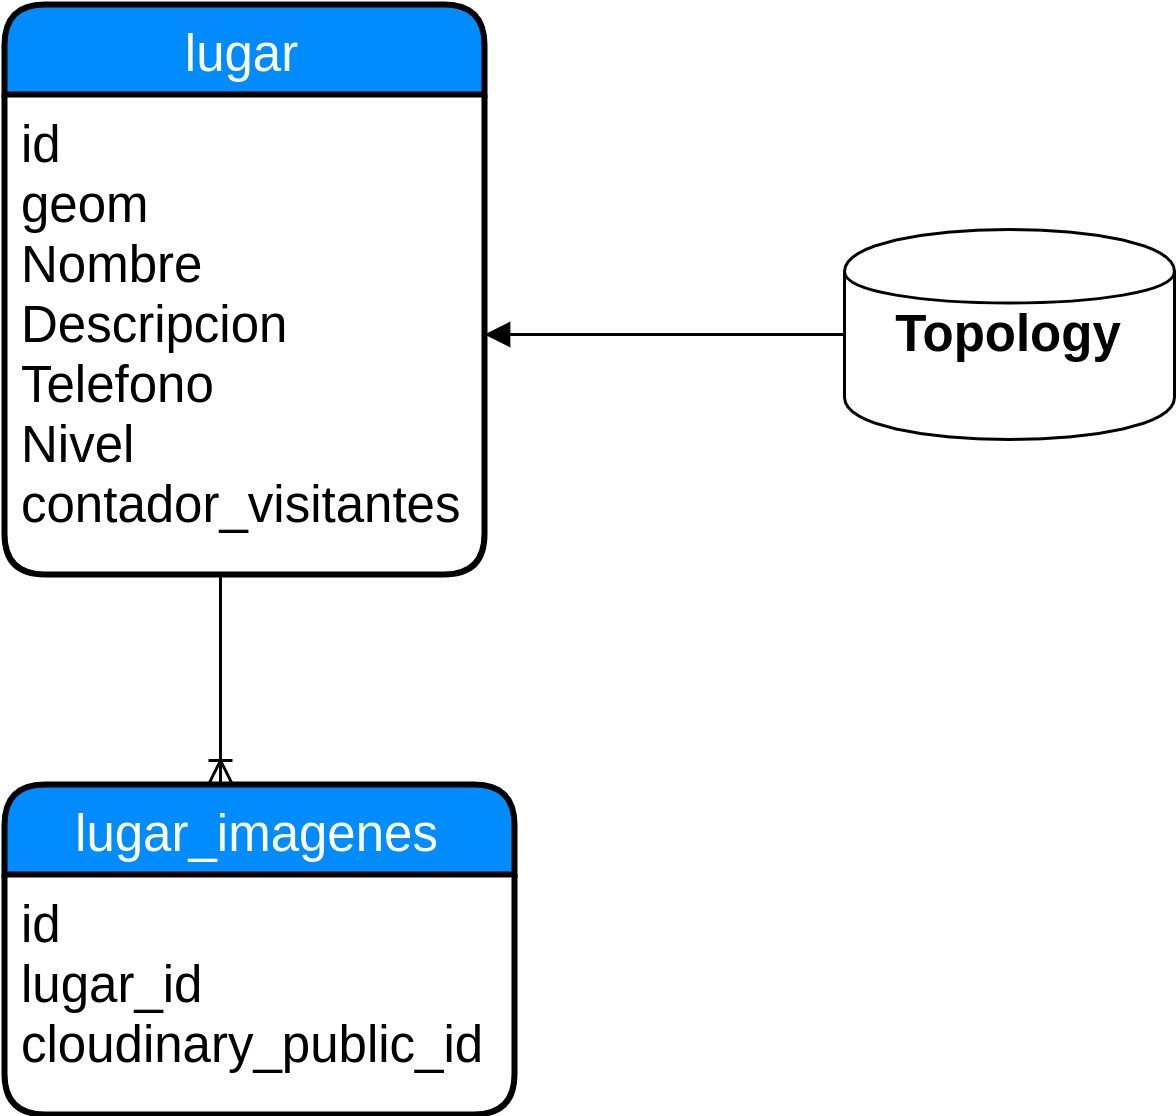
\includegraphics[width=0.4\textwidth]{diagramas/er_lugar}
  \end{center}
  \caption{Diagrama ER: Lugares}
  \label{fig:er_lugar}
  \caption*{Fuente: Elaboración propia}
\end{figure}



\item \textbf{Diagrama de Secuencia:}

En la figura \ref{fig:sequence_ver_lugar}, se observa el diagrama de secuencia correspondiente obtención de la lista e información de lugares.


\begin{figure}[H]
  \begin{center}
    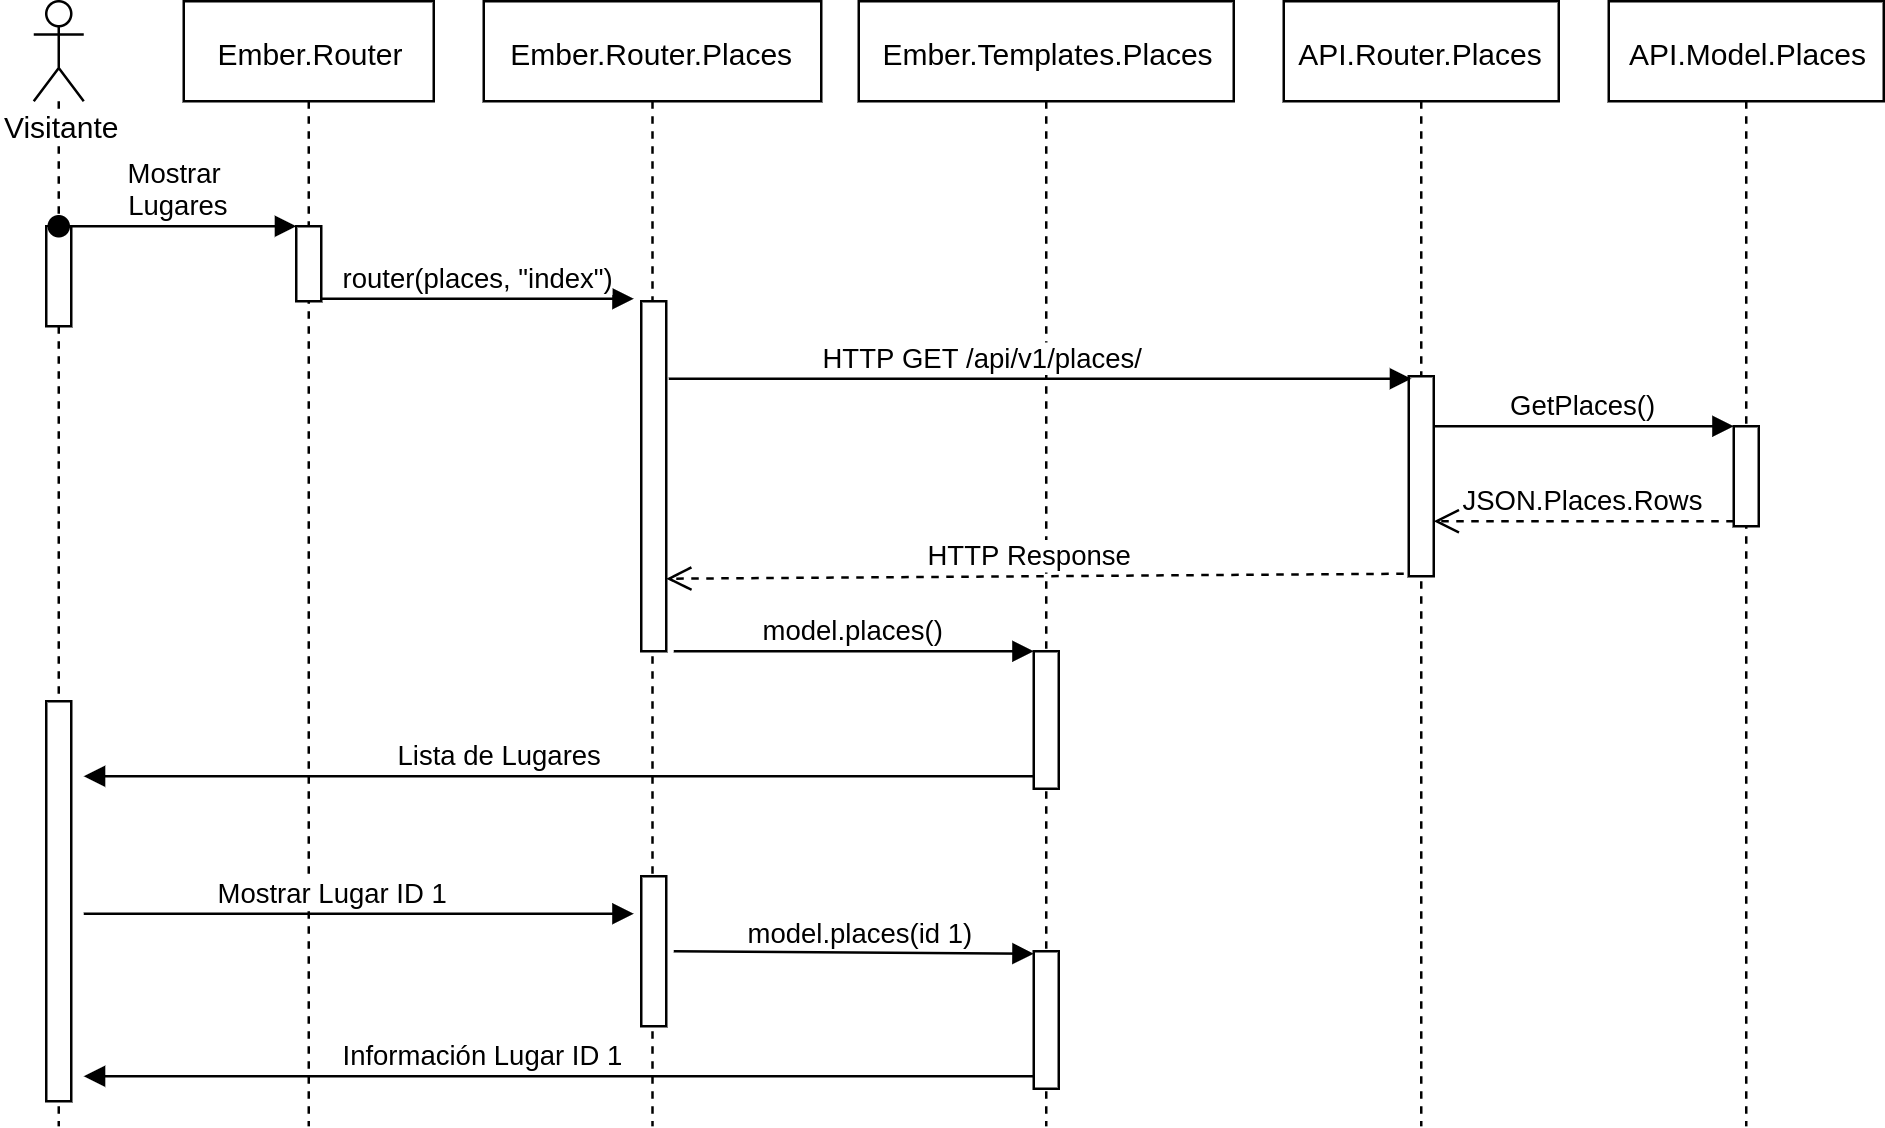
\includegraphics[width=0.9\textwidth]{diagramas/sequence_ver_lugar}
  \end{center}
  \caption{Diagrama de Secuencia: Lista e Información de Lugares}
  \label{fig:sequence_ver_lugar}
  \caption*{Fuente: Elaboración propia}
\end{figure}



\item \textbf{Diagrama de Clases:}


En la figura \ref{fig:clases_lugares}, se observa el diagrama de clases correspondiente a los lugares y la información de estos.

\begin{figure}[H]
\begin{center}
  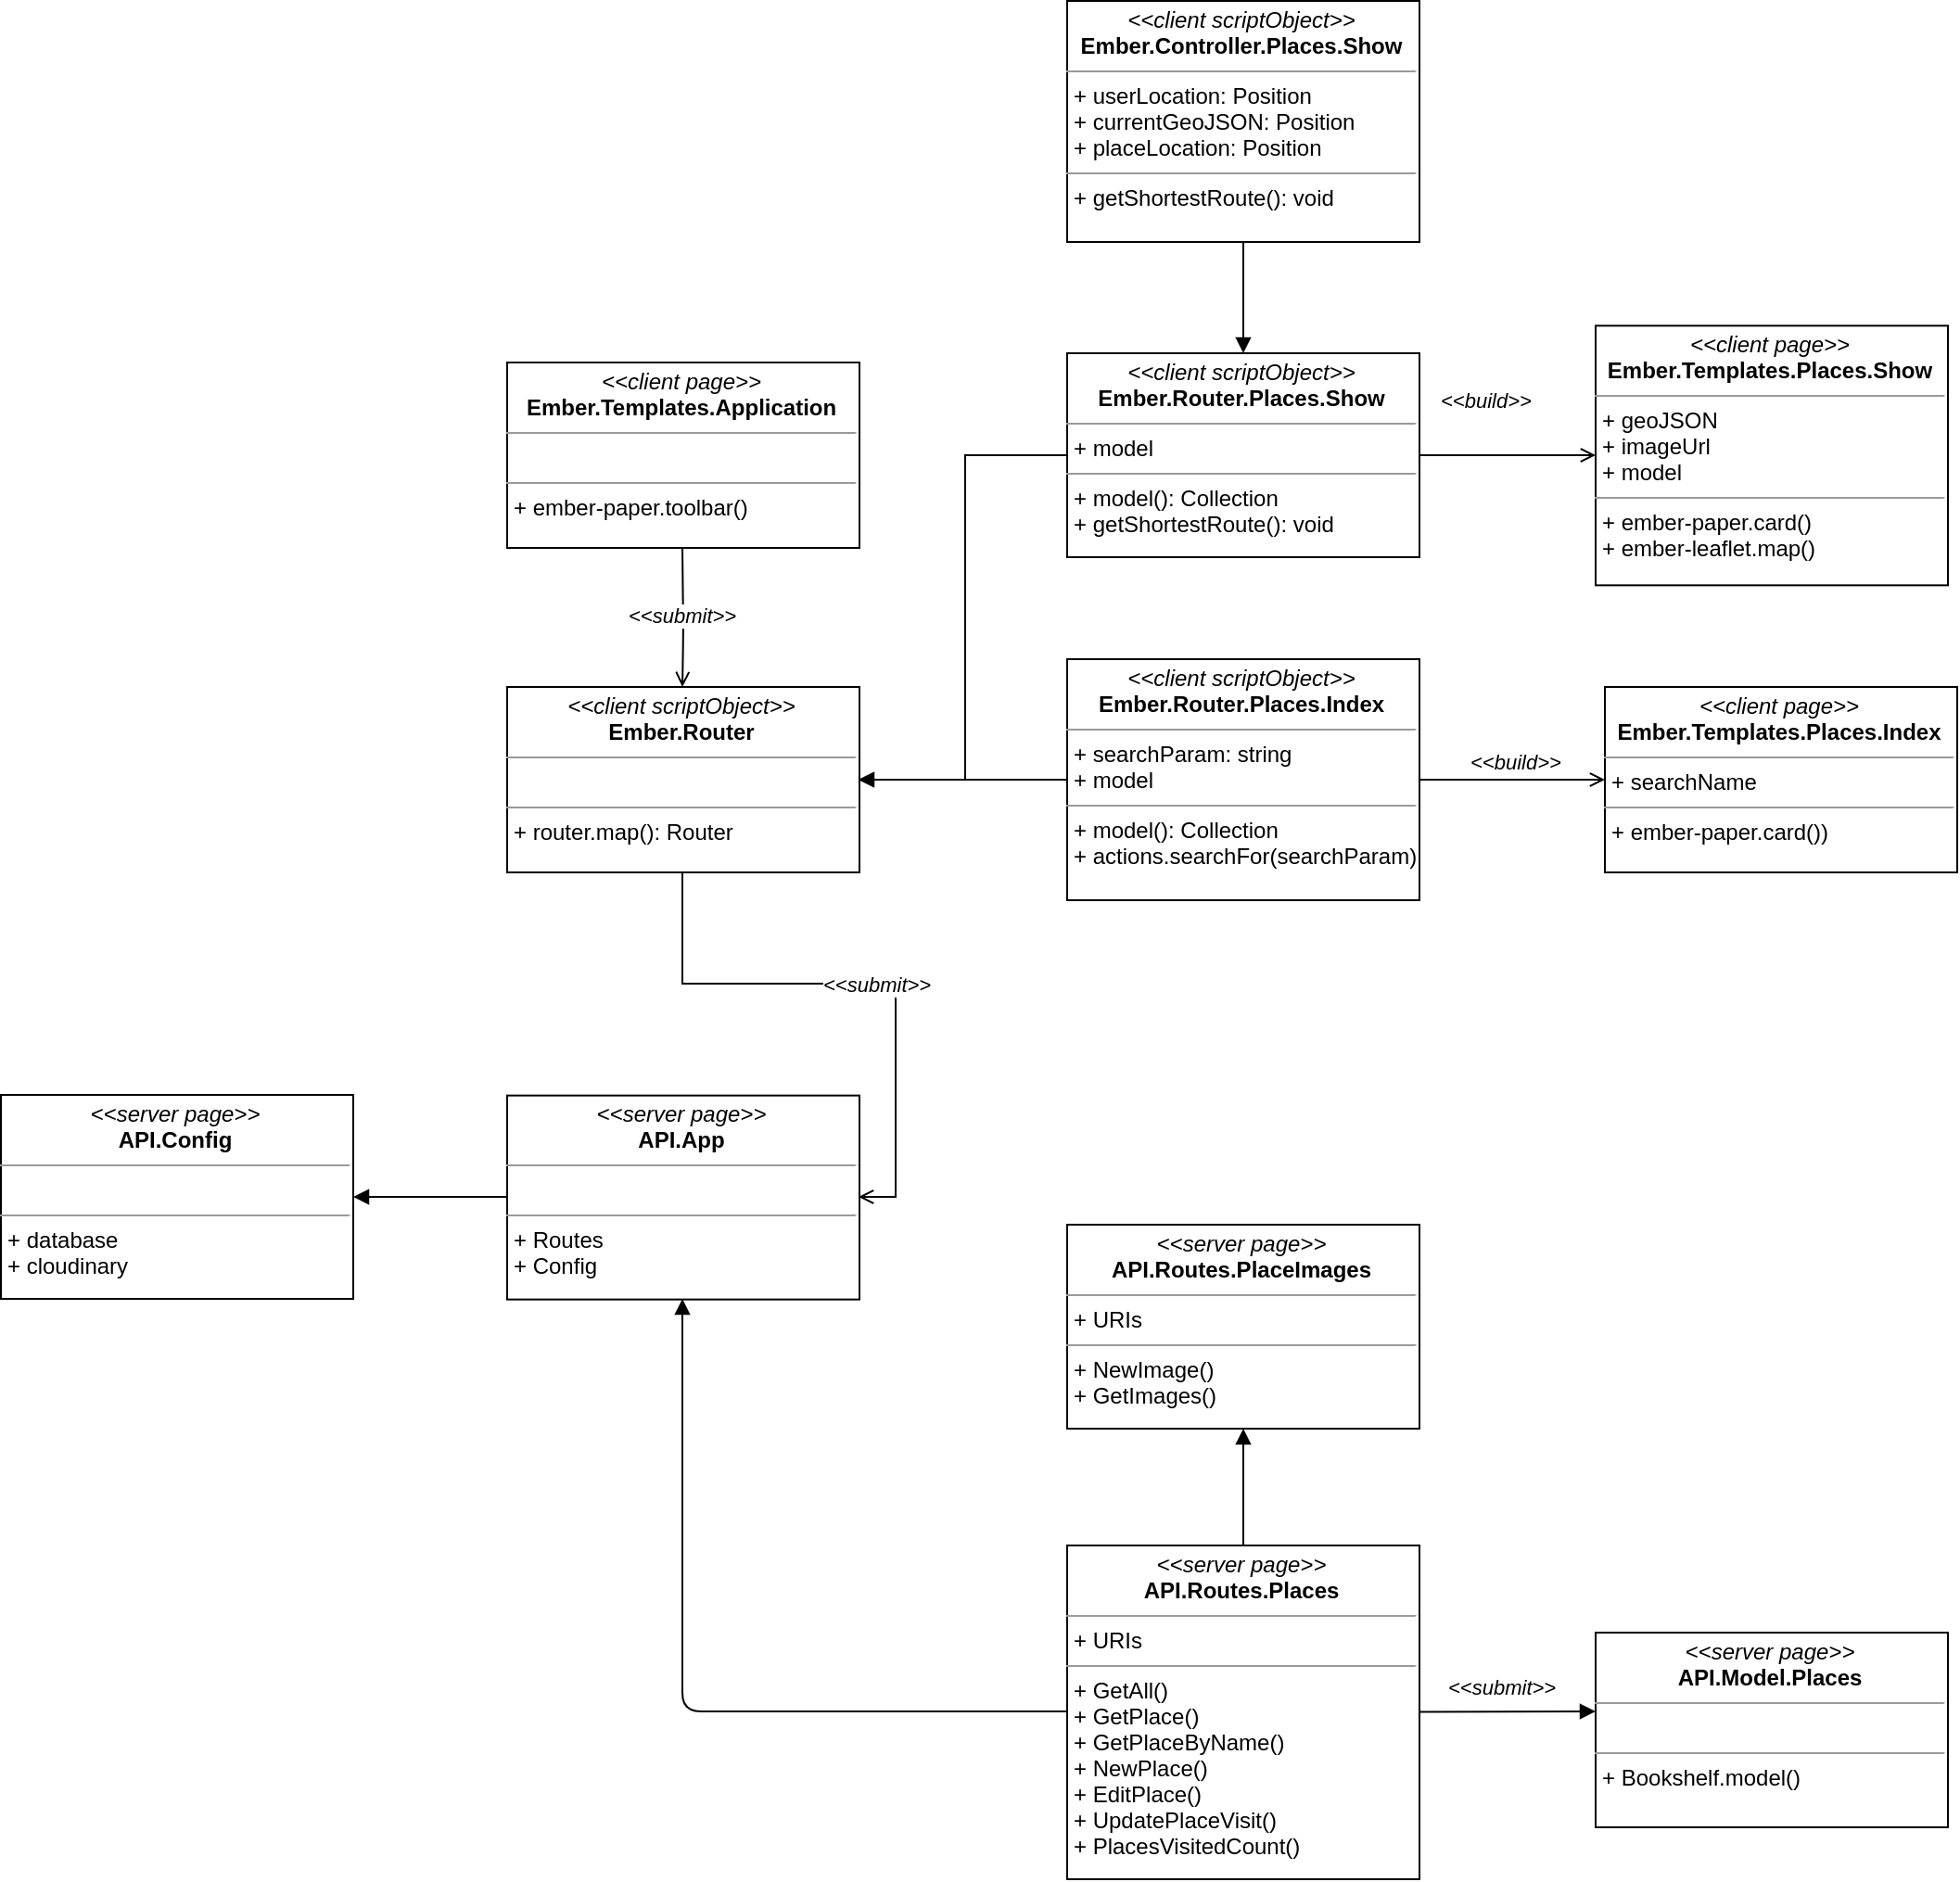
\includegraphics[width=0.9\textwidth]{diagramas/clases_lugares}
\end{center}
\caption{Diagrama de Clases: Lugares}
\label{fig:clases_lugares}
\caption*{Fuente: Elaboración propia}
\end{figure}


\end{itemize}


\subsection{Implementación}
% \label{sub:implementacion_iteracion_1}

    \subsubsection{Recolecion de la informacion de los lugares}
% \label{subs:Los lugares}

En primer lugar se recolectó la información de los lugares que la aplicación contendrá  de forma inicial, al igual que para recolectar las rutas se hizo uso de un \emph{GPS Garmin Nuvi 1300}, el cual cuenta con la opción de guardar locaciones como favoritos, entonces solo fue necesario estar cerca del lugar que se desea guardar y activar esa opción del GPS, este guarda la información en un archivo \emph{.gpx} y con la ayuda de \emph{QGIS} se genero el archivo shapefile correspondiente.\\

Posteriormente es necesario pasar la información geoespacial del shapefile a la base de datos, para esta tarea se hizo uso de una herramienta disponible para postgres, \emph{shp2pgsql}, que permite la conversión de un archivo shapefile a un archivo sql.

% $ shp2pgsql -s 4326 -I -S -c -d ~/Documents/places.shp > places.sql
\begin{verbatim}
  $ shp2pgsql -s 3785 -I -S -c -d ~/Documents/places.shp > places.sql
\end{verbatim}

Con el anterior comando se tiene como resultado un archivo \emph{.sql}, el cual es ingresado en la base de datos ya configurada, de esta forma nuestra base de datos para a contener una tabla geoespacial con datos de tipo \emph{POINT}, los cuales representan los lugares dentro del campus de la UMSS.\\

% \begin{verbatim}
%   $ shp2pgsql -s 4326 -I -S -c -d ~/Documents/ways.shp > ways.sql
% \end{verbatim}
%
% De la misma forma es necesario pasar la información de las rutas contenidas en un archivo shapefile a un archivo sql, en este caso creará una tabla \emph{WAYS}.\\

El archivo \emph{sql} resultante es usado para popular la base de datos con la información inicial de los lugares que contiene el campus universitario, para tal tarea se usó el siguiente comando.\\
% Los archivos resultantes \emph{sql} son usados para popular la base de datos .\\

\begin{verbatim}
  $ psql -d db_ubikate -U db_admin -f /Documents/places.sql
\end{verbatim}

\begin{figure}[H]
  \begin{center}
    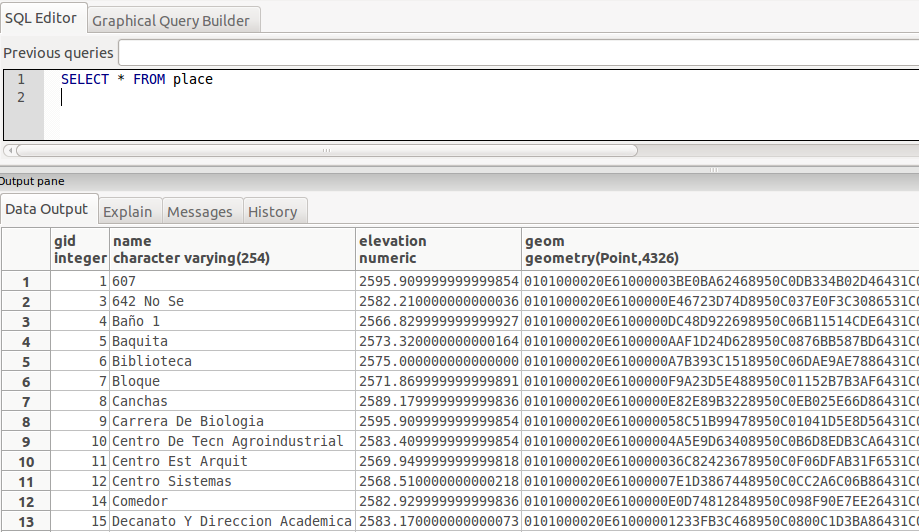
\includegraphics[width=1\textwidth]{iteration1/postgres_places}
    \caption{Herramienta gráfica de PostgreSQL (\emph{pgAdmin}).}
    \label{fig:postgres_places}
    \caption*{Fuente: Elaboración propia}
  \end{center}
\end{figure}
 % con la tabla de Lugares desplegada.

En la figura \ref{fig:postgres_places} se puede observar que la columna \emph{Elevation} contiene datos que el GPS Garmin Nuvi 1300 genera al momento de guardar un punto, en el presente caso es irrelevante.\\


Una vez que se tiene populada la base de datos con la informacion de los lugares es necesario implementar el como se comunicara el backend con el frontend, este como ya se explico se implementara un Servicio Web basado en un API REST.\\



\subsubsection{Implementación del REST API}
\label{subs:Implementacion del REST API}



El servidor necesita reconocer las peticiones que le llegan del cliente, para lo cual es necesario ``mapear'' un URI a una acción específica, las cuales ya están preparadas para comunicarse con la base de datos, no hay restricción en la declaración de las URIs pero para una mejor comprensión del API que se está desarrollando es necesario seguir convenciones que aseguran que cualquier desarrollador pueda comprender el API presentado y pueda ser fácilmente consumido por cualquier aplicación que requiera acceder a la información que disponible, un API REST es el que cumple con estas características.
En primer lugar es necesario crear las URIs que serán ``entendidas'' por el servidor, esto se logra declarando en el servicio creado con \emph{Express.JS}, tal como se puede apreciar en el siguiente bloque de código, cada URI se lo relaciona a un modelo en específico de acuerdo a la acción que se requiere, tal como se puede observar en el cuadro \ref{tab:rest} las URIs declaradas en el API cumplen con tal característica.\\


% \begin{minted}{js}[label=express_api,caption=Declarando API REST con ExpressJS]
\begin{center}
  \begin{lstlisting}[label=express_api,caption=Declarando API REST con ExpressJS]

        const router = express.Router();
        router.get('/', places.getAll);
        router.get('/:id', places.getPlace);
        router.post('/', places.newPlace);
        router.put('/:id', places.editPlace);
        router.delete('/:id', places.deletePlace);

        app.use('/api/v1/places', router);

  \end{lstlisting}
\end{center}
% \end{minted}

% En el código

  %
  % Para lograr todo este comportamiento  es necesario declarar, en el archivo
  % que controla las rutas dentro de la aplicación, \textbf{routes}, que el
  % recurso \textbf{user} es \emph{restful}, tal como se muestra en la figura \ref{fig:rest}\\

  % \begin{figure}[!hbp]
  %   \begin{center}
  %     \caption[REST - routes.rb]{config/routes.rb}
  %     \label{fig:rest}
  %     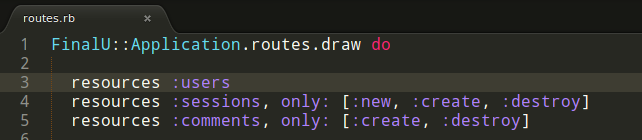
\includegraphics[width=1\textwidth]{rest}
  %     \caption*{Fuente: }
  %   \end{center}
  % \end{figure}

  El cuadro \ref{tab:rest} muestra como se puede leer las peticiones al API de \textbf{places}, las acciones mostradas son las que se pueden encontrar en un API REST pero no es necesario declararlas todas para considerar a que un API es restful.\\


  \begin{table}[H]
    \begin{center}

      \begin{tabularx}{0.75\textwidth}{ l l l  X }
        \toprule
        \multicolumn{1}{c}{\textbf{HTTP}} &
        \multicolumn{1}{c}{\textbf{URI}}  &
        % \multicolumn{1}{c}{\textbf{C}}  &
        \multicolumn{1}{c}{\textbf{ACCI\'ON}} &
        \multicolumn{1}{c}{\textbf{USADO PARA}}  \\
        \multicolumn{1}{c}{\textbf{request}} & & & \\

        \midrule
        GET     &  /places    &  index    & devuelve una lista con todos los lugares\\
        POST    &  /places    &  create   & inserta un nuevo lugar en la bd\\
        GET     &  /places/1  &  show     & muestra el lugar con identificador \emph{1}\\
        PUT     &  /places/1  &  update   & actualiza los datos de un lugar específico\\
        DELETE  &  /places/1  &  delete   & elimina el lugar con id = 1 de la bd\\
        \bottomrule
      \end{tabularx}

      \caption[recursos REST]{REST URIs para los lugares}
      \label{tab:rest}

      \caption*{Fuente: Elaboración propia}
    \end{center}
  \end{table}

  % Tal como se ve en el cuadro \ref{tab:rest}, Rails maneja los request HTTP de acuerdo con
  % el tipo de llamada que se realice, este trabajo lo realiza el \textbf{router},
  % que reconoce las URLs y los despacha a una \textbf{acción} del controlador,
  % todo este proceso ya está implementado en el núcleo de Rails por lo tanto  es automático y el programador
  % no necesita más configuración que la mostrada en la figura \ref{fig:rest},
  % obedeciendo al principio de \emph{Convención sobre configuración}\\

  % % no son más que métodos dentro del \emph{user\_controller.rb}
  % el cual
  % es parte del controlador de la arquitectura MVC.\\

  % The Rails router recognizes URLs and dispatches them to a controller’s action. It can also generate paths and URLs, avoiding the need to hardcode strings in your views.

  Por ejemplo, si se genera una petición GET hacia la direccion
  \mbox{\emph{/places/1}}  el servidor interpreta la dirección y responde
  mostrando la información del lugar “1” y en cambio si se genera
  una petición \emph{PUT} a la misma direccion \emph{/places/1} se ejecuta la acción \textbf{update} y se actualizan los datos del lugar ``1''. \\

  % \textbf{usuarios} actualizando la información del usuario “1”. \\

  Siguiendo la convención de un API REST ayuda a entender el flujo que tiene un recurso,
  las URL son legibles y únicos para cada recurso. Por lo tanto la implementación   de los recursos se hace de forma más limpia y ordenada, situaciones que son   claves para el mantenimiento y la extensibilidad del sistema. \\


Una vez implementado el servicio web, necesitamos empezar con el desarrollo del frontend de la aplicacion, que como ya se explico se usara \emph{EmberJS} para esta tarea. \\


\subsubsection{Mostrar los lugares}


\emph{EmberJS} tiene que consumir la informacion del API implementado, por lo tanto se hara una llamada \emph{GET} al URI \emph{places/}, dentro de la estructura de \emph{EmberJS} se tiene que implementar en el \emph{Router} dedicado al URI correspondiente. El siguiente metodo es el encarado de hacer la llamada y obtener la lista de lugares del API

\begin{center}
  \begin{lstlisting}[label=model_places_index,caption=Obtener la lista de lugares del API]

    model() {
        var url = (ENV.APP.API_HOST || '') + '/api/v1/places/';
        return jQuery.ajax({
          url: url,
          type: 'GET'
        });
      }

  \end{lstlisting}
\end{center}

Una vez obtenido la lista de lugares es necesario para el visitante que la lista este disponible en el navegador, para lo cual se usara el \emph{template} de \emph{EmberJs} correspondiente al URI, \emph{templates/places/index.hbs}.

\begin{center}
  \begin{lstlisting}[label=template_places_index,caption=Template de la lista de lugares]

    {{#paper-list}}
      {{#each model.data as |place|}}
        {{#paper-item class="md-1-line" onClick=(transition-to 'places.show' place)}}
            <div class="md-list-item-text">
                <span>{{place.name}}</span>
            </div>
        {{/paper-item}}
        {{paper-divider}}
      {{/each}}
    {{/paper-list}}

  \end{lstlisting}
\end{center}

En la anterior implementacion se hizo uso de \emph{ember-paper}, que como ya se explico ayudara en el ``look and feel'' de la aplicacion, el cual se puede observar en la figura \ref{fig:places_index}, la lista de lugares es mostrada en el navegador en un dispositivo movil.


\begin{figure}[H]
  \begin{center}
    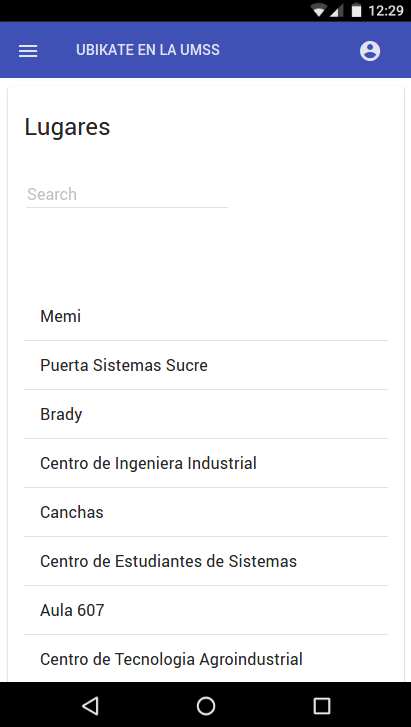
\includegraphics[width=0.3\textwidth]{iteration1/places_index_2}
    \caption{Lista de Lugares}
    \label{fig:places_index}
    \caption*{Fuente: Elaboración propia}
  \end{center}
\end{figure}


\subsubsection{Busqueda de los lugares}
\label{subs:busqueda de los lugares}

Para la implementacion de la busqueda de los lugares, un de los criterios de aceptacion es que sea posible la busqueda usando el nombre del lugar o parte del mismo, es necesario anadir un \emph{URI} adicional a nuestro servicio web, que obtenga de la base de datos un conjunto de lugares que concuerden con el criterio de busqueda, a continuacion se puede ver el URI implementado en la servicio web. \\

\begin{center}
  \begin{lstlisting}[label=endpoint_search_place,caption=Implementacion de la busqueda de lugares en el Servicio Web]

    router.get('places/search/:name', places.getPlacesByName);

  \end{lstlisting}
\end{center}


\subsubsection{Mostrar informacion del lugar}
\label{subs:Mostrar informacion del lugar}

La obtencion de la informacion de un lugar corresponde al URI \emph{places/:id} usando el verbo HTTP \emph{GET}, el cual obtiene la informacion en formato JSON, entonces se necesita mostrar esta informacion en el navegador, para lo cual el template correspondente al URI llegaria a ser \emph{templates/places/show}.

\begin{center}
  \begin{lstlisting}[label=template_places_show,caption=Template para mostrar la informacion de un lugar]
      {{#text.headline}}{{model.name}}{{/text.headline}}
      {{#card.content}}
          {{#paper-list}}
              {{model.description}}
              {{/paper-item}}
                  {{paper-icon "local_phone"}} {{model.phone}}
              {{/paper-item}}
              {{#paper-item class="md-2-line" }}
                  {{paper-icon "layers"}} Piso N# {{model.level}}
              {{/paper-item}}
          {{/paper-list}}
      {{/card.content}}

  \end{lstlisting}
\end{center}

El resultado del template renderizado en el navegador se puede apreciar en la figura \ref{fig:place_show}.

\begin{figure}[H]
  \begin{center}
    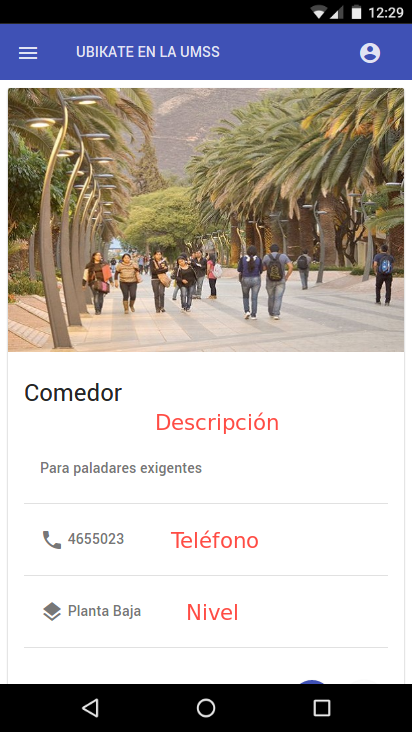
\includegraphics[width=0.3\textwidth]{iteration1/place_show}
    \caption{Vista de la Información de un Lugar.}
    \label{fig:place_show}
    \caption*{Fuente: Elaboración propia}
  \end{center}
\end{figure}




% En la figura \ref{fig:places_index}, se puede observar un


\subsection{Pruebas de Aceptación}

\begin{table}[H]
  \begin{center}
    \begin{tabularx}{0.75\textwidth}{ X }
      \toprule
      \textbf{Codigo:} CP001
      \makebox[3cm][r]{}
      \makebox[6cm][r]{\textbf{Historia de Usuario:} US01} \\

      \addlinespace
      \textbf{Nombre:} Verificar la lista de lugares. \\

      \addlinespace
      \textbf{Descripción:} Validar que un usuario visitante puede ver la lista de lugares cuando ingresa al menú \emph{lugares}. \\

      \addlinespace
      \textbf{Condiciones de Ejecución:} \\
      \tab \textbf{a.} El usuario no debe estar registrado. \\
      \tab \textbf{b.} Deben existir lugares registrados en el sistema.\\

      \addlinespace
      \textbf{Entradas / Pasos de Ejecución:}  \\
      \tab \textbf{1.} Hacer tap sobre el botón \emph{menú} en la esquina superior-izquierda. \\
      \tab \textbf{2.} Seleccionar el menú \emph{lugares}.\\

      \addlinespace
      \textbf{Resultado Esperado:} El Usuario debe ver una lista con los lugares registrados en la Condición de Ejecución \emph{b}.  \\

      \addlinespace
      \textbf{Evaluación de la Prueba:} Prueba exitosa. \\

      \bottomrule
    \end{tabularx}
    \caption{Prueba de Aceptación - CP001}
    \label{tab:CP001}
  \end{center}
\end{table}

\begin{table}[H]
  \begin{center}
    \begin{tabularx}{0.75\textwidth}{ X }
      \toprule
      \textbf{Codigo:} CP002
      \makebox[3cm][r]{}
      \makebox[6cm][r]{\textbf{Historia de Usuario:} US01} \\

      \addlinespace
      \textbf{Nombre:} Verificar la busqueda de lugares. \\

      \addlinespace
      \textbf{Descripción:} Validar que un usuario puede filtrar un lugar de la lista mediante el nombre. \\

      \addlinespace
      \textbf{Condiciones de Ejecución:} Ingresar en la base de datos el lugar con nombre ``MEMI''. \\

      \addlinespace
      \textbf{Entradas / Pasos de Ejecución:}  \\
      \tab \textbf{1.} Hacer tap sobre el botón \emph{menú} en la esquina superior-izquierda. \\
      \tab \textbf{2.} Seleccionar el menú \emph{lugares}.\\
      \tab \textbf{3.} Ingresar el nombre ``MEMI'' en el cajón de búsqueda.\\


      \addlinespace
      \textbf{Resultado Esperado:} Se debe mostrar un solo item en la lista de lugares con el nombre ``MEMI'' desplegado.\\

      \addlinespace
      \textbf{Evaluación de la Prueba:} Prueba exitosa. \\

      \bottomrule
    \end{tabularx}
    \caption{Prueba de Aceptación - CP002}
    \label{tab:CP002}
  \end{center}
\end{table}

\begin{table}[H]
  \begin{center}
    \begin{tabularx}{0.75\textwidth}{ X }
      \toprule
      \textbf{Codigo:} CP003
      \makebox[3cm][r]{}
      \makebox[6cm][r]{\textbf{Historia de Usuario:} US02} \\

      \addlinespace
      \textbf{Nombre:} Verificar la información de un lugar. \\

      \addlinespace
      \textbf{Descripción:} Validar que un usuario puede ver la descripción, el teléfono, el nivel y la foto de un lugar. \\

      \addlinespace
      \textbf{Condiciones de Ejecución:} Ingresar en la base de datos el lugar con nombre ``MEMI'' con su información completa. \\

      \addlinespace
      \textbf{Entradas / Pasos de Ejecución:}  \\
      \tab \textbf{1.} Hacer tap sobre el botón \emph{menú} en la esquina superior-izquierda. \\
      \tab \textbf{2.} Seleccionar el menú \emph{lugares}.\\
      \tab \textbf{3.} En la lista de lugares seleccionar el item ``MEMI''.\\

      \addlinespace
      \textbf{Resultado Esperado:} Se debe mostrar una pantalla con la foto del lugar ``MEMI'', su descripción, el teléfono y el nivel.\\

      \addlinespace
      \textbf{Evaluación de la Prueba:} Prueba exitosa. \\

      \bottomrule
    \end{tabularx}
    \caption{Prueba de Aceptación - CP003}
    \label{tab:CP003}
  \end{center}
\end{table}



\subsubsection{Resultado de las pruebas de la Iteración 1}

Al finalizar la Iteración 1, se ejecutaron todas las pruebas escritas durante la presente iteración, en el cuadro \ref{tab:regresion_1} se puede ver el detalle.


\begin{table}[H]
  \begin{center}
    \begin{tabularx}{0.8\textwidth}{ c  X  c }
      \toprule
        \textbf{Código} &
        \multicolumn{1}{c}{\textbf{Título de la Prueba}} &
        \textbf{Resultado}\\

      \midrule
        CP001
        &
        Verificar la lista de lugares.
        &
        Exitoso \\

\addlinespace
CP002
&
Verificar la busqueda de lugares.
&
Exitoso \\

\addlinespace
CP003
&
Verificar la información de un lugar.
&
Exitoso \\

\addlinespace
CP004
&
Verificar la lista de lugares cuando se busca un lugar no registrado.
&
Exitoso \\

\addlinespace
CP005
&
Verificar la información de un lugar mediante el URI.
&
Exitoso \\

\addlinespace
CP006
&
Verificar que el \emph{Menú} sea desplegado dinámicamente.
&
Exitoso \\



      \bottomrule
    \end{tabularx}
    \caption{Pruebas de regresión de la Iteración 1}
    \label{tab:regresion_1}
  \end{center}
\end{table}


\begin{itemize}
  \item Se ejecutaron 5 pruebas de funcionalidad, todas pasaron exitosamente.
  \item Se ejecutó 1 prueba de usabilidad, pasó exitosamente.
\end{itemize}


\section{Iteración 2}
\label{sec:iteracion_2}

Después de que finalizó la primera iteración y ya que todas las pruebas pasaron exitosamente, se continúa con la segunda iteración.


\subsection{Iteration Planning Meeting}
\label{sub:iteration2_planning_meeting}


Al igual que la primera iteración, las fases de exploración y planeación se realizan al mismo tiempo, en el sentido que no es necesario repartir las tareas resultantes de la exploración, por lo tanto al mismo tiempo en que se determinan las tareas se puede realizar la estimación de las mismas.

  \subsubsection{Exploración y Planeación}
  \label{subs:iteration2_exploracion_planeacion}

  Para la segunda iteración se toman en cuenta todas las historias de usuario restantes, y de acuerdo al criterio de escoger las siguientes historias más relevantes y de mayor valor para el producto, se escogió la historia de usuario #4.\\

  Como parte de la fase de Exploración se toma la historia de usuario #4 y la dividimos en las Tareas de Ingeniería, las cuales serán trabajadas en la fase de la Implementación.

  En la siguente tabla se especificaran las tareas correspondientes a la historia de usuario #4 \ref{tab:us04_tasks}. \\

  \subsection{Tareas del US04}
  \label{sub:us04_tasks}

    \begin{table}[H]
  \begin{center}
    \begin{tabularx}{\textwidth}{ c  X  C{2.3cm} }
      \toprule
        \textbf{Código} &
        \multicolumn{1}{c}{\textbf{Tarea}} &
        \textbf{Estimación [dias]}\\

      \midrule
        T011
        &
        Crear un archivo shapefile con información inicial de lugares principales dentro el campus de la UMSS.
        &
        2 \\

      \addlinespace
        T012
        &
        Preparar la base de datos para manejar información geográfica de rutas.
        &
        1 \\
      %
      % \addlinespace
      %   T013
      %   &
      %   Investigar e instalar una herramienta que permita usar un servicio de mapas.
      %   &
      %   1 \\

      % \addlinespace
      %   T014
      %   &
      %   El usuario puede ver un mapa usando un servicio del campus de la UMSS.
      %   &
      %   0.5 \\

      % \addlinespace
      %   T015
      %   &
      %   El usuario puede ver un marcador sobre el lugar.
      %   &
      %   0.5 \\
      %
      % \addlinespace
      %   T016
      %   &
      %   El marcador tiene información básica del lugar, nombre, piso.
      %   &
      %   0.5 \\

      \addlinespace
        T017
        &
        El usuario puede ver un marcador mostrando el lugar actual donde se encuentra (el usuario).
        &
        0.5 \\

      \addlinespace
        T018
        &
        Desarrollar un módulo que encuentra la ruta más corta usando la base de datos con información geográfica ruteable de T012.
        &
        2 \\

      \addlinespace
        T019
        &
        El usuario puede ver una línea roja que une el marcador de la posición del usuario con el marcador del lugar.
        &
        1 \\

      % \addlinespace
      %   TS003
      %   &
      %   Crear pruebas de funcionalidad del US04.
      %   &
      %   1 \\

      \addlinespace
      \midrule
        & \multicolumn{1}{R{7cm}}{\textbf{Total: }}
        & 10 \\

      \bottomrule
    \end{tabularx}
    \caption{Tareas del US04}
    \label{tab:us04_tasks}
  \end{center}
\end{table}


  \subsection{Calendario de Entregas}
  \label{subs:schedule_2}

    % \begin{table}[!ht]
%
% \end{table}
\begin{table}[H]

  \begin{center}

\begin{ganttchart}[
  canvas/.append style={fill=none, draw=black!5, line width=.75pt},
  hgrid style/.style={draw=black!5, line width=.75pt},
  vgrid={*1{draw=black!5, line width=.75pt}},
  %today=0,
  % today label=Semana 3,
  today rule/.style={
    draw=black!64,
    dash pattern=on 3.5pt off 4.5pt,
    line width=1.5pt
  },
  today label font=\small\bfseries,
  title/.style={draw=none, fill=none},
  title label font=\bfseries\footnotesize,
  title label node/.append style={below=7pt},
  include title in canvas=false,
  bar label font=\mdseries\small\color{black!70},
  bar label node/.append style={left=2cm},
  bar/.append style={draw=none, fill=black!63},
  bar incomplete/.append style={fill=barblue},
  bar progress label font=\mdseries\footnotesize\color{black!70},
  group incomplete/.append style={fill=groupblue},
    group left shift=0,
    group right shift=0,
    group height=.5,
    group peaks tip position=0,
    group label node/.append style={left=.6cm},
    group progress label font=\bfseries\small,
    link/.style={-latex, line width=1.5pt, linkred},
    link label font=\scriptsize\bfseries,
    link label node/.append style={below left=-2pt and 0pt},
  ]{1}{12}
  \gantttitle{Calendario de Entregasde de la Iteración 2}{7} \\[grid]
  \gantttitle{Semana 1}{7}
  \gantttitle{Semana 2}{7} \\
  % \gantttitle{Noviembre}{4} \\
  \gantttitle[title label node/.append style={below left=7pt and -3pt}]{D\'ia:\quad15}{0}
  \gantttitlelist{16,...,30}{1} \\
  % \ganttgroup[progress=0]{Historias de Usuario}{1}{8} \\
  \ganttbar[
    progress=0,
    name=bar1
  ]{\textbf{User Story 04}}{1}{12} \\
  % \ganttbar[
  %   progress=0,
  %   name=bar2
  % ]{\textbf{User Story 03}}{10}{12} \\
  % \ganttbar[
  %   progress=0,
  %   name=bar3
  % ]{\textbf{Iteración 3}}{5}{6} \\
  % \ganttbar[
  %   progress=0,
  %   name=bar4
  % ]{\textbf{Iteración 4}}{7}{8} \\
  % \ganttbar[
  %   progress=100,
  %   name=bar5
  % ]{\textbf{Actividad 5}}{5}{7} \\
  % \ganttbar[
  %   progress=80,
  % ]{\textbf{Actividad 6}}{8}{8} \\
  % \ganttbar[
  %   progress=49,
  % ]{\textbf{Actividad 7}}{9}{11} \\
  % \ganttmilestone{Hito 1}{11}{11}  \\
  % \ganttmilestone{Hito 2}{12}{12} \\
  %

  % \ganttmilestone{Q6 report}{24}{24} \\
  % \ganttmilestone{M1: Project finished}{8}{8}

  % \ganttlink[link type=f-s]{bar1}{bar2}
  % \ganttlink[link type=f-s]{bar2}{bar3}
  % \ganttlink[link type=f-s]{bar3}{bar4}

\end{ganttchart}

\caption{Calendario de Entregas de la Iteración 2}
\label{tab:calendario_entregas_iteracion_2}

\end{center}
\end{table}



\subsection{Implementación}
\label{sub:implementacion_iteracion_1}

Durante esta fase es donde se implementaran las tareas especificadas en la tabla \ref{tab:us04_tasks}.

\subsubsection{RF011}
\label{subs:RF011}

% Crear un archivo shapefile con la información geográfica de las rutas internas del campus de la UMSS

% Como ya se explico en \ref{sec:ruta_corta_umss}, esta tarea se llevo a cabo recabando la informacion geoespacial con un dispositivo GPS y exportando los datos resultantes a un archivo shapefile, el cual se puede apreciar en \ref{fig:shapefile_umss_v1}.

\subsubsection{RF012}
\label{subs:RF012}

% Preparar la base de datos para manejar información geográfica de rutas

% Para realizar esta tarea se procedió a instalar pgRouting, el resultado de esta tarea se puede apreciar en el manual de instalación ## \\
%
% Una vez configurada la base de datos se procede a cargar la misma con la informacion obtenida en RF011, para tal efecto es necesario primeramente crear una tabla que contendra los LINESTRING contenidos en el shapefile, esta operacion es similar a la realizada en la tarea - RF003 (\ref{sub:RF003}). Una vez que ya se tiene la tabla a la llamamos \emph{ways}, se necesita ejecutar un query propio de \emph{pgRouting} el cual tiene como objetivo analizar los datos geo-espaciales de la tabla y a\~nadirle una \emph{topologia}.
%
% Dentro lo que es la \emph{topologia geoespacial} existe una aplicacion que se lo conoce como \emph{topología de red}. La \emph{topología de red} representa las relaciones entre segmentos en una red lineal o una colección de segmentos de línea\cite{osgeo_journal_topology}.
% En un \emph{SIG} la topologia ayuda a mejorar el analisis de datos geo-espaciales, para resolver el problema de la ruta corta \emph{pgRouting} genera una \emph{topología de red} usando los datos que existen en la tabla \emph{ways}, es necesario ejecutar una instruccion, la que se muestra a continiacion y \emph{pgRouting} se encarga de llenar los datos que se pueden observar en la figura \ref{fig:postgres_ways}, las columnas \emph{source} y \emph{target} son populadas con el analisis topologico y en la figura \ref{fig:postgres_vertices}, se puede observar que la tabla \emph{ways\_vertices\_pgr} es creada enteramente en la ejecucion de la instruccion.
%
% \begin{verbatim}
%   select pgr_createTopology('ways', 0.00000001, 'geom', 'gid');
% \end{verbatim}
%
% \begin{figure}[H]
%   \begin{center}
%     \caption{Vista de la tabla \emph{ways} en la base de datos PostgreSQL.}
%     \label{fig:postgres_ways}
%     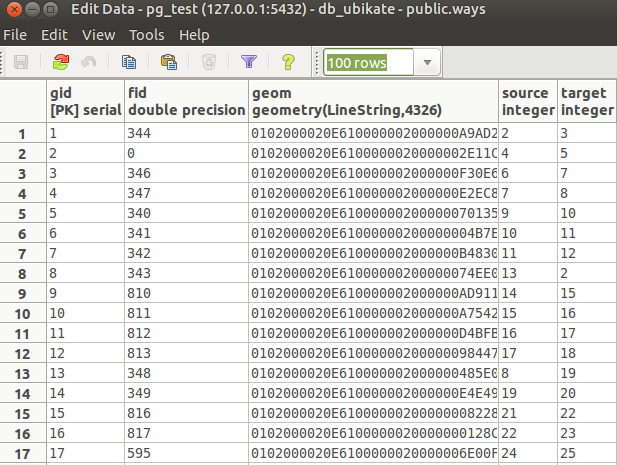
\includegraphics[width=1\textwidth]{iteration2/postgres_ways}
%     \caption*{Fuente: Elaboración propia}
%   \end{center}
% \end{figure}
%
% En la figura \ref{fig:postgres_ways} se puede apreciar que cada fila es una parte de la línea original obtenida por el dispositivo GPS y explisionada por QGIS, hay que notar que las columnas \emph{source} y \emph{target} hacen referencia a los nodos o vertices que la primera linea tiene en sus extremos, la primera linea o fila esta identificada por la columna \emph{gid}.\\
%
% En la siguiente figura \ref{fig:postgres_vertices} se observa la tabla \emph{ways\_vertices\_pgr} que contiene los vertices creados a partir del analisis de los datos en la tabla \emph{ways}.
%
% \begin{figure}[H]
%   \begin{center}
%     \caption{Vista de la tabla \emph{ways\_vertices\_pgr} en la base de datos PostgreSQL.}
%     \label{fig:postgres_vertices}
%     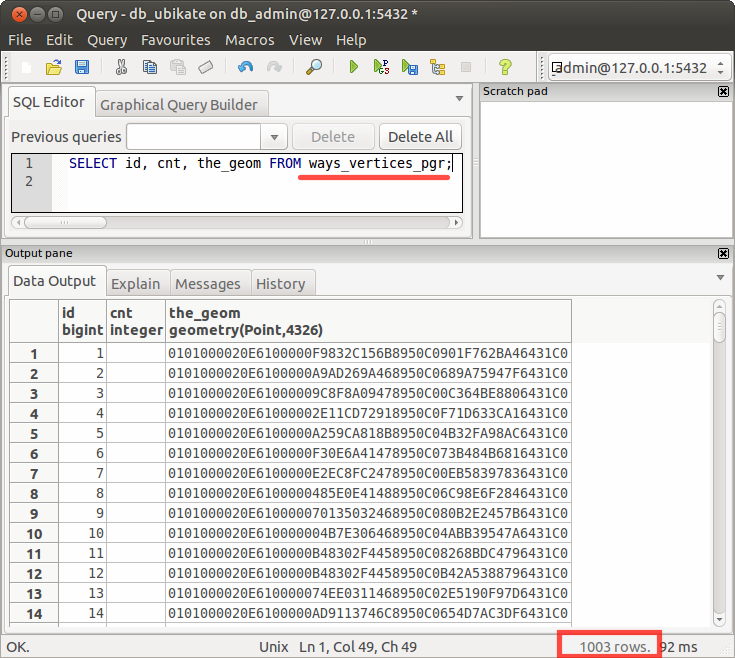
\includegraphics[width=1\textwidth]{iteration2/postgres_vertices}
%     \caption*{Fuente: Elaboración propia}
%   \end{center}
% \end{figure}
%
% Para entender los datos generados hay leer la informacion de las 2 tablas, por ejemplo en la primera  fila (gid 1) de la tabla \emph{ways}, se observa que el contenido de la columna \emph{source} es igual a \textbf{2} y \emph{target} es igual a \textbf{3}, eso quiere decir que los vertices del LINESTRING de la fila 1 son los vertices con \textbf{id} 2 y 3 respectivamente de la tabla \emph{ways\_vertices\_pgr}.\\
%
%
% Todo el conjunto de vertices y lineas de estas tablas se podria representar con una Matriz de adyacencias, explicada en \ref{sub:representacion_de_un_grafo}, y usada en la resolucion de la ruta mas corta, mas especificamente con el algoritmo de Dijkstra.

\subsubsection{RF013}
\label{subs:RF013}

% Investigar e instalar una herramienta que permita usar un servicio de mapas
% Durante la investigacion de esta tarea se encontro \emph{ember-leaflet}, una libreria o plugin que contiene las herramientas para poder cargar y usar un servicio de mapas.\\
%
% Para instalar esta libreria solo se necesita ejecutar el siguiente comando y posteriormente ya se puede empezar a utilizarla.\\
%
% \begin{verbatim}
%   $ ember install ember-leaflet
% \end{verbatim}
%
% El resultado de la investigacion puede apreciar en el marco teórico, en la sección que describe la librería, \emph{ember-leaflet}. \ref{sec:ember_js}

\subsubsection{RF014}
\label{subs:RF014}

% El usuario puede ver un mapa usando un servicio del campus de la UMSS

% Para completar esta tarea se hizo uso de la herramienta \emph{ember-leaflet}, con la cual se puede desplegar un mapa en el browser y optimizada para dispositivos moviles.\\
%
% \begin{verbatim}
%   {{#leaflet-map lat=lat lng=lng zoom=zoom}}
%     {{tile-layer
%       url="http://{s}.tile.openstreetmap.fr/hot/{z}/{x}/{y}.png"
%     }}
%   {{/leaflet-map}}
% \end{verbatim}
%
% Con la anterior instrucción se accede al servicio de \emph{Open Street Maps}, de la cual obtenemos los datos necesarios para renderizar un mapa en el browser. Los atributos de \emph{lat} y \emph{lng} se acceden de la capa del controlador de la aplicacion, son la latitud y longitud respectivamente, la convinacion de ambos datos es la locacion donde se va a ubicar el renderizado del mapa.\\

% Esta librería es la nos ayudará a insertar fácilmente los marcadores que irán sobre los lugares o la líneas que mostraran la ruta más corta
%
% Como resultado de esta tarea se puede apreciar la siguiente figura,

\subsubsection{RF015}
\label{subs:RF015}
% El usuario puede ver un marcador sobre el lugar

% Para completar esta tarea se continuó usando la librería \emph{ember-leaflet}, la cual permite que con la siguiente instrucción se despliegue un marcador sobre el mapa renderizado del API de \emph{Open Street Maps}.
%
% \begin{verbatim}
%   {{#marker-layer location=userLocation}} {{/marker-layer}}
% \end{verbatim}
%
% El resultado de la tarea se puede observar en la figura \ref{fig:baquita_place}.

\subsubsection{RF016}
\label{subs:RF016}
% marcador se  tiene información básica del lugar, nombre, piso

% Para poder mostrar la informacion del lugar sobre el marcador creado en RF015 se hizo uso de la librería \emph{ember-leaflet}, al igual que dicha tarea, solo se necesito de una instruccion para poder desplegar la informacion necesaria.
%
% \begin{verbatim}
%   {{#marker-layer location=location}}
%     h3>{{model.name}}</h3>
%     {{model.description}}
%     <strong>telf:</strong> {{model.phone}}
%     <strong>piso#</strong> {{model.level}}
%   {{/marker-layer}}
% \end{verbatim}
%
% En la figura \ref{fig:baquita_place} se puede apreciar el marcador con la información desplegada del lugar ``Baquita''.
%
% \begin{figure}[H]
%   \begin{center}
%     \caption{Tooltip con la información de un lugar.}
%     \label{fig:baquita_place}
%     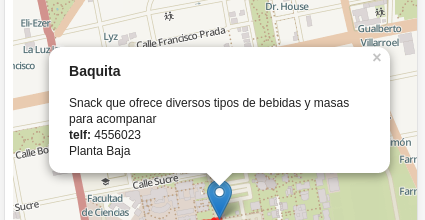
\includegraphics[width=1\textwidth]{iteration2/baquita_place}
%     \caption*{Fuente: Elaboración propia.}
%   \end{center}
% \end{figure}


\subsubsection{RF017}
\label{subs:RF017}
% El usuario puede ver un marcador mostrando el lugar actual donde se encuentra (el usuario)

% Para encontrar la locación del usuario se uso el API de geolocalización propio de HTML5, que en un smarthphone puede acceder y usar los recursos nativos de un smartphone, es necesaria la aceptacion del usuario mediante un mensaje que el navegador desplega, la locacion es encontrada mediante la triangulacion de Coordenadas por GPS (el mas exacto a la hora de encontrar la locacion del dispositvo), Wi-Fi, GSM o CDMA. Solo es necesaria la ejecucion de la siguente linea para ponder obetener la posición actual del usuario usando el API de geolocalización de HTML5.
%
% \begin{verbatim}
%   var coords = Geolocation.getCurrentPosition();
%   var latitud = coords.latitude;
%   var longitud = coords.longitude;
% \end{verbatim}
%
% La \emph{latitud} y \emph{longitud} obtenidas es fácilmente trasladado al mapa usando \emph{ember-leaflet} mediante un marcador, como se puede apreciar en la siguiente figura.
%
% \begin{figure}[H]
%   \begin{center}
%     \caption{Tooltip con la latitud y longitud de la posición actual del usuario.}
%     \label{fig:location_marker}
%     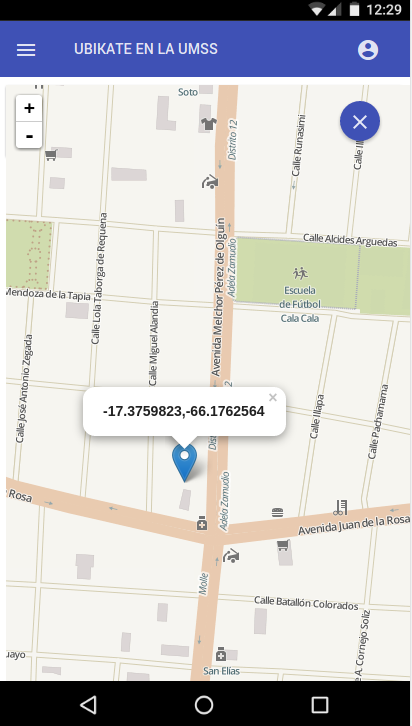
\includegraphics[width=0.5\textwidth]{iteration2/location_marker}
%     \caption*{Fuente: Elaboración propia.}
%   \end{center}
% \end{figure}

\subsubsection{RF018}
\label{subs:RF018}
% Desarrollar un módulo que encuentra la ruta más corta usando la base de datos con información geográfica ruteable de RF012

% Durante esta tarea se investigó la mejor forma de encontrar la ruta más corta y se llegó a la conclusión de usar la combinación de \emph{Postgres + Postgis + pgRouting}, esta investigación se puede apreciar en el marco teórico.\\
%
% Para hallar la ruta más corta se necesita usar las características de la base de datos para poder analizar los datos geográficos almacenados en la Tarea RF012, como el análisis que se requiere hacer es caro osea el costo de procesador para realizar los calculos necesarios es elevado, lo mas recomendable es que este trabajo sea realizado en el backend de la aplicacion por la base de datos.\\
%
% Tambien hay que tomar en cuenta que la tierra no es plana y las líneas que en un mapa parecen lineas rectas, realmente no son rectas, ya que el planeta Tierra es un \emph{esferoide oblato}\footnote{Un \emph{esferoide oblato} (o elipsoide oblato) es un elipsoide de revolución obtenido por rotación de una elipse alrededor de su eje más corto.} por lo que las lineas en apariencia rectas tienen la curvatura natural del planeta Tierra. En distancias largas esto tiene un gran impacto al manejar o utilizar mapas projectados, pero tambien es cierto que para una área pequeña como es el campus de la Universidad de San Simón este problema no tiene un gran impacto pero no está demás en tomar en cuenta esta característica del análisis de datos geoespaciales, como se explico en el capitulo \ref{cha:geolocalizacion}, para el presente proyecto se usara el proyeccion \emph{SRID 3857}.\\

% Una vez que se tienen en cuanta estas variables es necesaria la resolucion del problema de la ruta más corta, \emph{pgRouting} tiene varios métodos implementados para el analisis de datos geo-espaciales en la resolucion de este problema, para el presente proyecto se usara el algoritmo de \emph{Dijkstra}, explicado en el capítulo \ref{cha:ruta_optima}.\\
%
% Tomando en cuenta los conceptos aprendidos y las herramientas investigadas es que se desarrollo el modulo que encuentra la ruta mas corta.

% La siguiente SQL query está diseñado y explicado en la documentación de pgRouting {ref - link}, básicamente se necesita especificar el nodo inicio y el nodo destino y la base de datos se encarga de analizar la tabla creada en RF012, para que el algoritmo de Dijkstra funcione hay que darle un Costo a cada uno de los tramos pertenecientes a la Matriz, en este caso el costo será la longitud del tramo(st_length(geom) AS cost),  el costo de ir del punto A al punto B puede no ser la misma que de ir del punto B al punto A a pesar de ser una única línea, por ejemplo si la circulación fuera en un solo sentido  como en el caso de las rutas para automoviles, en este caso como es una ruta peatonal se simplifica un poco el problema, entonces como datos de entrada tenemos el punto donde se encuentra el usuario extraído por RF017 y el punto del lugar buscado extraído por RF0##, tomando en cuenta estos datos se armó el siguiente query,

% var raw = "SELECT seq, id1 AS node, id2 AS edge, cost " +
%             "FROM pgr_dijkstra('SELECT gid AS id, source::integer, target::integer, st_length(geom) AS cost " +
%             "                   FROM public.ways', " + targetId + ", " + sourceId + ", false, false);";

\subsubsection{RF019}
\label{subs:RF019}
% El usuario puede ver una línea roja que une el marcador de la posición del usuario con el marcador del lugar
% Como resultado de la tarea RF018 se tiene un conjunto de datos en formato de latitud y longitud que conforman líneas, las cuales representan la ruta más corta, pero al final es solo un montón de números, útiles pero para el usuario esta información es difícil de procesar, el usuario necesita información que sea fácil de entender y no existe mejor herramienta disponible para esta tarea que mostrar la \emph{ruta} de forma visual, esto quiere decir que se necesita mostrar la ruta sobre un \emph{mapa}, en la aplicación se usará \emph{ember-leaflet} para desplegar el mapa ofrecido por los servicios de OpenStreetMaps y también para mostrar ruta más corta mediante una línea de color rojo.\\
%
% Para resolver esta tarea se creó un servicio API usando ExpressJS, la cual se encarga obtener la información extraída de la base de datos y transformarla en un objeto JSON (GeoJSON), este objeto contiene la información geoespacial necesaria para ``dibujar'' la línea roja entre 2 puntos georeferenciados, uno de los cuales es el lugar al que se quiere llegar y el otro es la ubicación actual del usuario. \\
%
% \begin{verbatim}
%   ENV.APP.API_HOST + '/api/v1/ways/route/' + sourceData.id + '/' + targetData.id;
%
%   GET /api/v1/ways/route/930/77 200 276.217 ms - 3911
%
%   $ curl http://localhost:3000/api/v1/ways/route/930/77 | python -m json.tool                                                       [3:04:52]
%   % Total    % Received % Xferd  Average Speed   Time    Time     Time  Current
%                                  Dload  Upload   Total   Spent    Left  Speed
% 100  3911  100  3911    0     0   161k      0 --:--:-- --:--:-- --:--:--  166k
% {
%     "features": [
%         {
%             "geometry": {
%                 "coordinates": [
%                     [
%                         -66.1467397848201,
%                         -17.3935321732846
%                     ],
%                     [
%                         -66.1467190789842,
%                         -17.3935294725234
%                     ]
%                 ],
%                 "type": "LineString"
%             },
%             "type": "Feature"
%         },
%
% \end{verbatim}
% % /api/v1/ways/route/
%
% % Este objeto es representado en el mapa usando ember-leaflet con la siguiente instrucción,
% %
% % {{#geojson-layer geoJSON=currentGeoJSON color='red' }}
% % {{/geojson-layer}}
%
% Y se puede observar en el mapa una línea roja que representa la ruta más corta entre el punto donde se encuentra el usuario y el punto del lugar a buscar.
%
% \begin{figure}[H]
%   \begin{center}
%     \caption{Ruta más corta dibujada con una línea roja.}
%     \label{fig:short_way_place}
%     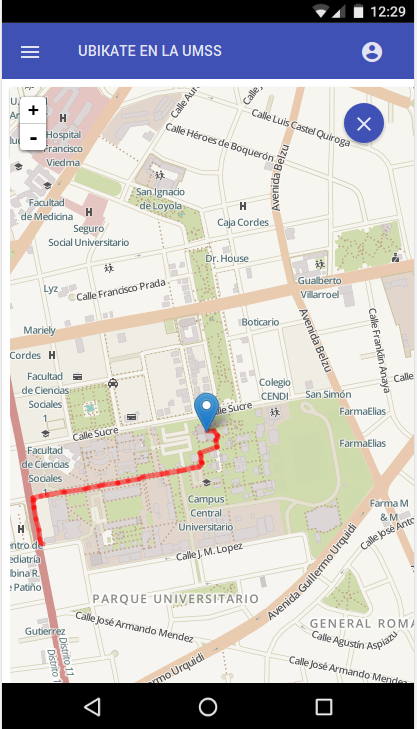
\includegraphics[width=0.5\textwidth]{iteration2/short_way_place}
%     \caption*{Fuente: Elaboración propia.}
%   \end{center}
% \end{figure}

\subsubsection{TS004}
\label{subs:TS004}

Pruebas funcionales

\subsection{Registrar el Avance}
\label{sub:iteracion2_avance}

\subsection{Verificación}
\label{sub:iteracion2_verificacion}

\section{Iteración 3}
\label{sec:iteracion_3}

% Al igual que al principio de la segunda iteración, se esperan los resultados de las pruebas realizadas para poder empezar con la planificación de la tercera iteración.

% \subsection{Iteration Planning Meeting}
% \label{sub:iteration2_planning_meeting}


% Los resultados de las pruebas realizadas se analizan para determinar si los criterios de aceptación, de las historias de usuario trabajadas en la segunda iteración, se cumplen para poder continuar con las historias que continúan sin ser desarrolladas, en caso que las pruebas fallen, es necesario continuar con la implementación de las historias inconclusas.\\
%
% En el caso del presente proyecto, las pruebas pasaron exitosamente y se aceptaron los criterios de aceptación de las historias de usuario trabajadas, por lo tanto se procede con la primera fase del “Iteration Planning”. \\

%
% \subsection{Exploración y Planeación}
% \label{sub:iteration2_exploracion_planeacion}

% Esta fase generalmente se realiza en 2 pasos pero será realizada al mismo tiempo, ya que en la exploración se definen las tareas a realizar y en la planeación se asigna estas tareas al equipo de desarrollo, el cual tiene que estimar las tareas, pero como el equipo de desarrollo está compuesto por mi persona, puedo definir las tareas y asignarles una estimación en el mismo paso.\\
%
% Para la Iteración 3, se trabajarán las historias de usuario 6 y 7, de las que a continuación se definirán sus tareas de ingeniería. \\


\subsection{Planificación de la Iteración 3}

  A continuación se analizará la \emph{historia de usuario} US06, ver el cuadro \ref{tab:US06}.

    
\begin{table}[H]
\begin{center}
  \begin{tabularx}{0.75\textwidth}{ X }
    \toprule
    \textbf{Historia de Usuario:} US06
    \makebox[6cm][r]{\textbf{Prioridad:} Alta} \\
    \makebox[4cm][r]{}
    \makebox[6cm][r]{\textbf{Riesgo:} Alto} \\

    \addlinespace
    \textbf{Nombre:} Añadir más lugares al sistema.\\

    \addlinespace
    \textbf{Descripción:} \\
    \tab Yo como usuario registrado.\\
    \tab Deseo añadir más lugares al sistema. \\
    \tab Para mejorar los criterios de busqueda. \\

    \addlinespace
    \textbf{Criterios de Aceptación:} \\
    \tab Quiero que sea posible anadir un lugar si no lo encuentro en la lista de lugares. \\
    \tab Quiero ver un formulario para poder ingresar los datos de un nuevo lugar.\\
    \tab Quiero pararme cerca o en el lugar que necesito añadir para georeferenciarlo. \\

    \bottomrule
  \end{tabularx}
  \caption{Historia de Usuario - US06}
  \label{tab:US06}
\end{center}
\end{table}


    \begin{table}[H]
  \begin{center}
    \begin{tabularx}{0.75\textwidth}{ X }
      \toprule
      \textbf{Número de Tarea:} T019
      \makebox[1cm][r]{}
      \makebox[6cm][r]{\textbf{Historia de Usuario:} US06} \\

      \addlinespace
      \textbf{Descripción:} Implementar en el backend el \emph{endpoint} para añadir y editar usuarios. \\

      \addlinespace
      \textbf{Tipo de Tarea:} Desarrollo
      \makebox[6cm][r]{\textbf{Estimación [dias]:} 1} \\

      \addlinespace
      \textbf{Programador Responsable:} Edmundo Figueroa \\

      \bottomrule
    \end{tabularx}
    \caption{Tarea de Ingeniería - T019}
    \label{tab:T019}
  \end{center}
\end{table}


\begin{table}[H]
  \begin{center}
    \begin{tabularx}{0.75\textwidth}{ X }
      \toprule
      \textbf{Número de Tarea:} T020
      \makebox[1cm][r]{}
      \makebox[6cm][r]{\textbf{Historia de Usuario:} US06} \\

      \addlinespace
      \textbf{Descripción:} Mostrar un botón para añadir lugares solamente a usuarios registrados. \\

      \addlinespace
      \textbf{Tipo de Tarea:} Desarrollo
      % \makebox[1cm][r]{}
      \makebox[6cm][r]{\textbf{Estimación [dias]:} 0.5} \\

      \addlinespace
      \textbf{Programador Responsable:} Edmundo Figueroa \\

      \bottomrule
    \end{tabularx}
    \caption{Tarea de Ingeniería - T020}
    \label{tab:T020}
  \end{center}
\end{table}

\begin{table}[H]
  \begin{center}
    \begin{tabularx}{0.75\textwidth}{ X }
      \toprule
      \textbf{Número de Tarea:} T021
      \makebox[1cm][r]{}
      \makebox[6cm][r]{\textbf{Historia de Usuario:} US06} \\

      \addlinespace
      \textbf{Descripción:} Mostrar un formulario para añadir más lugares, con el nombre del lugar, descripción, teléfono y nivel. \\

      \addlinespace
      \textbf{Tipo de Tarea:} Desarrollo
      \makebox[6cm][r]{\textbf{Estimación [dias]:} 0.5} \\

      \addlinespace
      \textbf{Programador Responsable:} Edmundo Figueroa \\

      \bottomrule
    \end{tabularx}
    \caption{Tarea de Ingeniería - T021}
    \label{tab:T021}
  \end{center}
\end{table}

\begin{table}[H]
  \begin{center}
    \begin{tabularx}{0.75\textwidth}{ X }
      \toprule
      \textbf{Número de Tarea:} T022
      \makebox[1cm][r]{}
      \makebox[6cm][r]{\textbf{Historia de Usuario:} US06} \\

      \addlinespace
      \textbf{Descripción:} Registrar las coordenadas del lugar al momento de crear un nuevo lugar. \\

      \addlinespace
      \textbf{Tipo de Tarea:} Desarrollo
      \makebox[6cm][r]{\textbf{Estimación [dias]:} 1} \\

      \addlinespace
      \textbf{Programador Responsable:} Edmundo Figueroa \\

      \bottomrule
    \end{tabularx}
    \caption{Tarea de Ingeniería - T022}
    \label{tab:T022}
  \end{center}
\end{table}


\begin{table}[H]
  \begin{center}
    \begin{tabularx}{0.75\textwidth}{ X }
      \toprule
      \textbf{Número de Tarea:} T023
      \makebox[1cm][r]{}
      \makebox[6cm][r]{\textbf{Historia de Usuario:} US06} \\

      \addlinespace
      \textbf{Descripción:} Implementar el modulo para poder agregar una foto a un lugar. \\

      \addlinespace
      \textbf{Tipo de Tarea:} Desarrollo
      \makebox[6cm][r]{\textbf{Estimación [dias]:} 1} \\

      \addlinespace
      \textbf{Programador Responsable:} Edmundo Figueroa \\

      \bottomrule
    \end{tabularx}
    \caption{Tarea de Ingeniería - T023}
    \label{tab:T023}
  \end{center}
\end{table}


  A continuación se analizará la \emph{historia de usuario} US07, ver el cuadro \ref{tab:US07}.

    
\begin{table}[H]
\begin{center}
 \begin{tabularx}{0.75\textwidth}{ X }
   \toprule
   \textbf{Historia de Usuario:} US07
   \makebox[6cm][r]{\textbf{Prioridad:} Alta} \\
   \makebox[4cm][r]{}
   \makebox[6cm][r]{\textbf{Riesgo:} Alto} \\

   \addlinespace
   \textbf{Nombre:} Editar la información de un lugar.\\

   \addlinespace
   \textbf{Descripción:} \\
   \tab Yo como usuario registrado.\\
   \tab Deseo editar la información de un lugar. \\
   \tab Para mejorar o corregir la información de ese lugar. \\

   \addlinespace
   \textbf{Criterios de Aceptación:} \\
   \tab Al entrar a la información de un lugar quiero ser el único que vea un icono para poder entrar a la edición de los datos. \\
   \tab Quiero acceder a un formulario que muestre la información actual del lugar y poder editar la información mostrada. \\

   \bottomrule
 \end{tabularx}
 \caption{Historia de Usuario - US07}
 \label{tab:US07}
\end{center}
\end{table}


    \begin{table}[H]
  \begin{center}
    \begin{tabularx}{0.75\textwidth}{ X }
      \toprule
      \textbf{Número de Tarea:} T024
      \makebox[1cm][r]{}
      \makebox[6cm][r]{\textbf{Historia de Usuario:} US07} \\

      \addlinespace
      \textbf{Descripción:} Implementar el modulo para editar lugares. \\

      \addlinespace
      \textbf{Tipo de Tarea:} Desarrollo
      \makebox[6cm][r]{\textbf{Estimación [dias]:} 1} \\

      \addlinespace
      \textbf{Programador Responsable:} Edmundo Figueroa \\

      \bottomrule
    \end{tabularx}
    \caption{Tarea de Ingeniería - T024}
    \label{tab:T024}
  \end{center}
\end{table}


\begin{table}[H]
  \begin{center}
    \begin{tabularx}{0.75\textwidth}{ X }
      \toprule
      \textbf{Número de Tarea:} T025
      \makebox[1cm][r]{}
      \makebox[6cm][r]{\textbf{Historia de Usuario:} US07} \\

      \addlinespace
      \textbf{Descripción:} Mostrar un botón para editar un lugar solamente a usuarios administradores. \\

      \addlinespace
      \textbf{Tipo de Tarea:} Desarrollo
      % \makebox[1cm][r]{}
      \makebox[6cm][r]{\textbf{Estimación [dias]:} 0.5} \\

      \addlinespace
      \textbf{Programador Responsable:} Edmundo Figueroa \\

      \bottomrule
    \end{tabularx}
    \caption{Tarea de Ingeniería - T025}
    \label{tab:T025}
  \end{center}
\end{table}

\begin{table}[H]
  \begin{center}
    \begin{tabularx}{0.75\textwidth}{ X }
      \toprule
      \textbf{Número de Tarea:} T026
      \makebox[1cm][r]{}
      \makebox[6cm][r]{\textbf{Historia de Usuario:} US07} \\

      \addlinespace
      \textbf{Descripción:} Mostrar la información actual del lugar en el formalario de edicion. \\

      \addlinespace
      \textbf{Tipo de Tarea:} Desarrollo
      \makebox[6cm][r]{\textbf{Estimación [dias]:} 0.5} \\

      \addlinespace
      \textbf{Programador Responsable:} Edmundo Figueroa \\

      \bottomrule
    \end{tabularx}
    \caption{Tarea de Ingeniería - T026}
    \label{tab:T026}
  \end{center}
\end{table}

\begin{table}[H]
  \begin{center}
    \begin{tabularx}{0.75\textwidth}{ X }
      \toprule
      \textbf{Número de Tarea:} T027
      \makebox[1cm][r]{}
      \makebox[6cm][r]{\textbf{Historia de Usuario:} US07} \\

      \addlinespace
      \textbf{Descripción:} Mostrar un boton para eliminar el lugar solamente a un usuario administrador. \\

      \addlinespace
      \textbf{Tipo de Tarea:} Desarrollo
      \makebox[6cm][r]{\textbf{Estimación [dias]:} 1} \\

      \addlinespace
      \textbf{Programador Responsable:} Edmundo Figueroa \\

      \bottomrule
    \end{tabularx}
    \caption{Tarea de Ingeniería - T027}
    \label{tab:T027}
  \end{center}
\end{table}



% \subsubsection{Tareas del US06}
% \label{sub:us06_tasks}

% \begin{table}[H]
  \begin{center}
    \begin{tabularx}{\textwidth}{ c  X  C{2.3cm} }
      \toprule
        \textbf{Código} &
        \multicolumn{1}{c}{\textbf{Tarea}} &
        \textbf{Estimación [dias]}\\

      \midrule
        T020
        &
        El usuario podrá ver un link hacia el formulario para añadir más lugares desde la lista de lugares existentes.
        &
        0.5 \\

      \addlinespace
        T021
        &
        El usuario podrá ver un formulario para añadir un lugar con información básica. por ejemplo, el nombre del lugar, descripción, teléfono.
        &
        1 \\

      \addlinespace
        T022
        &
        El usuario deberá estar cerca del lugar que desea añadir para poder georeferenciarlo.
        &
        1 \\

      \addlinespace
        T023
        &
        Un usuario no-administrador no debería poder ver el formulario para añadir lugares.
        &
        1 \\


      \addlinespace
        P004
        &
        Crear pruebas de funcionalidad del US05.
        &
        0.5 \\

      \addlinespace
      \midrule
        & \multicolumn{1}{R{7cm}}{\textbf{Total: }}
        & 4 \\

      \bottomrule
    \end{tabularx}
    \caption{Tareas del US05}
    \label{tab:us05_tasks}
  \end{center}
\end{table}

%
%
% \subsubsection{Tareas del US07}
% \label{sub:us07_tasks}

  % \begin{table}[H]
  \begin{center}
    \begin{tabularx}{\textwidth}{ c  X  C{2.3cm} }
      \toprule
        \textbf{Código} &
        \multicolumn{1}{c}{\textbf{Tarea}} &
        \textbf{Estimación [dias]}\\

      \midrule
      T024
      &
      Implementar en el backend el \emph{endpoint} para eliminar usuarios.
      &
      0.5 \\

      \addlinespace
        T024
        &
        Mostrar un boton solamente al administrador para editar un lugar.
        &
        0.5 \\

      \addlinespace
        T025
        &
        Mostrar la información actual del lugar en el formalario de edicion
        % El usuario debería poder ver la información actual del lugar en el formulario para editar el lugar.
        &
        1 \\

      \addlinespace
        T026
        &
        Mostrar un boton para eliminar el lugar solamente a un usuario administrador.
        % El usuario no-administrador no debería poder ver el link hacia el formulario para editar el lugar.
        &
        1 \\

      \addlinespace
        P005
        &
        Crear pruebas de funcionalidad del US06.
        &
        0.5 \\

      \addlinespace
      \midrule
        & \multicolumn{1}{R{7cm}}{\textbf{Total: }}
        & 3 \\

      \bottomrule
    \end{tabularx}
    \caption{Tareas del US06}
    \label{tab:us06_tasks}
  \end{center}
\end{table}



  % \subsection{Implementación}
  % \label{sub:implementacion_iteracion_3}

  \subsection{Implementación de la Iteración 3}


      
% \subsubsection{Implementar módulo para añadir lugares al sistema}
\subsubsection{Registro de Lugares en el sistema}

Para registrar un \emph{lugar} primeramente se implementó el formulario que se usará para recolectar la información del \emph{lugar}, el formulario fue creado usando \emph{EmberJs} y se lo puede ver en la figura \ref{fig:new_place}. \\

\begin{figure}[H]
     \begin{center}
       \includegraphics[width=0.3\textwidth]{new_place}

       \caption{Formulario para añadir un nuevo \emph{lugar}.}
       \label{fig:new_place}
       \caption*{Fuente: Elaboración propia.}
     \end{center}
\end{figure}

Posteriormente es necesario crear la petición HTTP desde el controlador de \emph{EmberJS} hacia el API, en el cuerpo de la petición se incluye la posición georeferenciada del celular utilizando el API de Geolocalización de HTML5 usada anteriormente para encontrar la ubicación del usuario, también se incluye el nombre, la descripción, el teléfono y el nivel del \emph{lugar}. En el codigo \ref{new_place_request} se puede ver la implementación de la petición.


% En la figura \ref{fig:new_place} se puede ver el formulario implementado usando \emph{ember-paper}, el cual colecciona los datos que se quieren introducir y se los envía al backend usando una llamada AJAX, como se puede ver en el siguiente código, para crear la petición POST se obtiene las coordenadas actuales del dispositivo móvil además de los datos recolectados del formulario y que con la ayuda de \emph{JQuery} es enviado al API el cual maneja la información recibida y se encarga de insertar los datos en la base de datos.\\

% \newpage
\begin{center}
 \begin{lstlisting}[label=new_place_request,caption=POST request creado en el controlador de \emph{ember}]

   var payload = {
       name: nombre,
       description: descripcion,
       phone: telefono,
       level: nivel,
       lat: latitud,
       lon: longitud
   };

   var url = (ENV.APP.API_HOST || '') + '/api/v1/places/';
   jQuery.post(url, payload).then(
       function(data) {
           var transition = controller.get('transition');
           if (transition) {
               self.transitionTo('places.show');
           } else {
               self.transitionTo('places');
           }
       },
       function(error) {
           controller.set('message', error.responseText);
       }
   );

 \end{lstlisting}
\end{center}

% En esta iteración se implementó la opción de añadir más lugares al sistema, de editarlos y eliminarlos, y la primera tarea es crear las consultas SQL para llevar a cabo las tareas. \\

% por lo que es necesario crear las consultas SQL que insertaran los datos enviados desde el dispositivo móvil al servidor. \\

% Como requisito para insertar un nuevo ``lugar'', se requiere que el usuario esté posicionado en el ``lugar'' ya que se usaran sus coordenadas para posicionar el ``lugar''. Las coordenadas del usuario son obtenidas usando el API de Geolocalización propia de HTML5, usada anteriormente para encontrar la ubicación del usuario \emph{visitante} en la iteración 2.\\

% Posteriormente se necesita implementar el formulario que el usuario usará para insertar los datos del ``lugar'': el nombre, la descripción, el teléfono y el nivel.\\

% Para insertar un ``lugar''  en la base de datos se usó el codigo \ref{new_place}, donde se puede observar la consulta SQL usada, para la cual se necesita capturar la latitud y longitud respectiva donde se encuentra el usuario, además de los datos del ``lugar''.\\

La petición creada es recibida en el API utilizando el \emph{endpoint} RESTful designado para ello, \verb|router.post('/', places.newPlace);|, el \emph{endpoint} se encarga de mandar la información recibida hacia la base de de datos, tomando en cuenta que la posición del lugar es un tipo especial de la base de datos, la latitud y longitud necesitan ser transformadas al momento de insertar el \emph{lugar} en la base de datos, como se muestra en el codigo \ref{cod-new_place_api}.


\begin{center}
 \begin{lstlisting}[label=cod-new_place_api,caption=Insertar un ``lugar'' en la base de datos.]

   router.post('/', places.newPlace);

   var newPlace = (req, res) => {
       var name = req.body.name || '';
       var lat = req.body.lat || '';
       var lon = req.body.lon || '';
       var description = req.body.description || '';
       var phone = req.body.phone || '';
       var level = req.body.level || '';

       let raw = `insert into place (name, geom, description, phone, level)
                  values ('${name}',
                          ST_GeomFromText('POINT(${lon} ${lat})', 3875),
                          '${description}',
                          '${phone}',
                          '${level}'
                         );`;

       Knex.raw(raw)
           .then(function(data) {
               res.json({
                   "message": "Place saved successfully!",
                   "data": data
               });
           })
           .catch(function(error) {
               res.send("Error:", error);
           });
   };

 \end{lstlisting}
\end{center}




% Para la creación de un ``lugar'' es necesario implementar un \emph{endpoint} en el API y siguiendo las convenciones REST se , para que como ya se explicó anteriormente el frontend pueda comunicarse con el backend. \\

% En el API de la aplicación, se implementó un \emph{endpoint} para que pueda manejar los \emph{request} del cliente para añadir un lugar, este \emph{request} es enviado usando el verbo HTTP \emph{POST}, que como ya se explicó es el usado en un REST API para crear objetos. \\

\subsubsection{Edición de la información del Lugar}

Para editar de la información de un lugar se rehusó el formulario ya creado para el registro del mismo, pero populando los campos con la información actual del lugar, el resultado se lo puede ver en la figura \ref{fig:place_edit_form}. \\

\begin{figure}[H]
     \begin{center}
       \includegraphics[width=0.3\textwidth]{place_edit_form}

       \caption{Formulario para editar un \emph{lugar}}
       \label{fig:place_edit_form}
       \caption*{Fuente: Elaboración propia.}
     \end{center}
\end{figure}


Los cambios a la información del \emph{lugar} son enviados al API mediante una petición PUT, siguiendo los lineamientos del REST API implementado, esta petición se puede ver en el codigo \ref{cod-edit_place_request}.

% \newpage
\begin{center}
 \begin{lstlisting}[label=cod-edit_place_request,caption=Petición HTTP para editar un lugar.]

   router.put('/:id', places.editPlace);

   var body = {
       name: name,
       description: description,
       phone: phone,
       level: level
   };

   var url = (ENV.APP.API_HOST || '') + `/api/v1/places/${id}`;
   jQuery.ajax({
       url: url,
       type: 'put',
       data: body
   }).then(
       function(data) {
           self.transitionTo('places.show', id);
       },
       function(error) {
           controller.set('message', error.responseText);
       }
   );

 \end{lstlisting}
\end{center}

A diferencia del registro del \emph{lugar}, que guarda la posición georeferenciada al momento de registrar el \emph{lugar}, en la edición de los datos no se está tomando en cuenta este dato porque se noto que generalmente cuando se requiere actualizar los datos del \emph{lugar}, el usuario no se encuentra en la posición original del \emph{lugar} y este dato se pierde, corrompiendo la base de datos. Es por esta razón que se decidió que no se actualizará la posición geográfica del \emph{lugar} sin alguna opción explícita que advierta al usuario de las consecuencias de esta acción, pero como tal tarea no se halla dentro de la \emph{historia de usuario} que se esta implementado, se tomo la decisión de realizarla en una futura iteración.








% \subsubsection{Eliminar un lugar}

% Una vez implementado la lógica para añadir un ``lugar'', se implementó los módulos para poder eliminar el ``lugar'', para esto se añadió un botón en la lista de lugares, el cual despliega un mensaje de advertencia al usuario de que está por eliminar un ``lugar'' y que la acción es irreversible, por lo tanto este botón sólo está disponible para un usuario \emph{administrador}. \\
%
% La verbo  HTTP \emph{DELETE} es el que de acuerdo a la implementación del API REST es el adecuado para eliminar un lugar, por lo tanto es el que se usó en la aplicación. En el codigo \ref{delete_place_enpoint} se puede observar el \emph{endpoint} implementado en el API que se encarga de manejar las peticiones \emph{DELETE} creando una consulta SQL que elimina el lugar de la base de datos.\\
%
% \begin{center}
%   \begin{lstlisting}[label=delete_place_enpoint,caption=DELETE request elimina un lugar.]
%
%     router.delete('/:id', places.deletePlace);
%
%     var deletePlace = (req, res) => {
%         var id = req.params.id;
%
%         Place.forge({
%             gid: id
%         })
%         .destroy()
%         .then(function(model) {
%             res.json({
%                 "message": "Place deleted successfully!"
%             });
%         })
%         .catch(function(err) {
%             res.status(500);
%         });
%     };
%
%   \end{lstlisting}
% \end{center}
%
% En el anterior codigo se puede apreciar la bondad de usar un manejador de bases de datos como \emph{Bookshelf} ya que usando el método \verb|destroy()|, se encarga automáticamente de crear la consulta SQL para eliminar una tupla de la base de datos.\\


  \subsection{Pruebas de Aceptación de la Iteración 3}

      \begin{table}[H]
  \begin{center}
    \begin{tabularx}{0.75\textwidth}{ X }
      \toprule
      \textbf{Codigo:} CP012
      \makebox[3cm][r]{}
      \makebox[6cm][r]{\textbf{Historia de Usuario:} US06} \\

      \addlinespace
      \textbf{Tipo:} Prueba de Funcionalidad - Positiva. \\

      \addlinespace
      \textbf{Nombre:} Verificar el registro de lugares. \\

      \addlinespace
      \textbf{Descripción:} Validar que un usuario registrado puede añadir un lugar nuevo al sistema. \\

      \addlinespace
      \textbf{Condiciones de Ejecución:} \\
      \tab \textbf{a.} El usuario debe estar registrado. \\
      % \tab \textbf{b.} Registrar un lugar dentro del campus Universitario.\\

      \addlinespace
      \textbf{Entradas / Pasos de Ejecución:}  \\
      \tab \textbf{1.} Seleccionar el menú \emph{Lugares}. \\
      \tab \textbf{2.} Hacer tap sobre el icono de registro de lugares.\\
      \tab \textbf{3.} Ingresar el Nombre del lugar.\\
      \tab \textbf{4.} Ingresar una Descripción del lugar.\\
      \tab \textbf{5.} Ingresar el Teléfono del lugar.\\
      \tab \textbf{6.} Ingresar el Nivel del lugar.\\
      \tab \textbf{7.} Aceptar el formulario.\\


      \addlinespace
      \textbf{Resultado Esperado:} Una vista de la información del lugar es desplegada con los datos ingresados en los pasos.  \\

      \addlinespace
      \textbf{Evaluación de la Prueba:} Prueba exitosa. \\

      \bottomrule
    \end{tabularx}
    \caption{Prueba de Aceptación - CP012}
    \label{tab:CP012}
  \end{center}
\end{table}

\begin{table}[H]
  \begin{center}
    \begin{tabularx}{0.75\textwidth}{ X }
      \toprule
      \textbf{Codigo:} CP013
      \makebox[3cm][r]{}
      \makebox[6cm][r]{\textbf{Historia de Usuario:} US07} \\

      \addlinespace
      \textbf{Tipo:} Prueba de Funcionalidad - Positiva. \\

      \addlinespace
      \textbf{Nombre:} Verificar la edición de la información de un lugar. \\

      \addlinespace
      \textbf{Descripción:} Validar que un usuario registrado puede editar la información de un lugar. \\

      \addlinespace
      \textbf{Condiciones de Ejecución:} \\
      \tab \textbf{a.} El usuario debe estar registrado. \\
      \tab \textbf{b.} Registrar un lugar dentro del campus Universitario.\\

      \addlinespace
      \textbf{Entradas / Pasos de Ejecución:}  \\
      \tab \textbf{1.} Seleccionar el menú \emph{Lugares}. \\
      \tab \textbf{2.} Buscar el lugar registrado en las condiciones.\\
      \tab \textbf{3.} Editar el Nombre del lugar.\\
      \tab \textbf{4.} Editar la Descripción del lugar.\\
      \tab \textbf{5.} Editar el Teléfono del lugar.\\
      \tab \textbf{6.} Editar el Nivel del lugar.\\
      \tab \textbf{7.} Aceptar el formulario.\\


      \addlinespace
      \textbf{Resultado Esperado:} Una vista de la información del lugar es desplegada con la información editada en los pasos.  \\

      \addlinespace
      \textbf{Evaluación de la Prueba:} Prueba exitosa. \\

      \bottomrule
    \end{tabularx}
    \caption{Prueba de Aceptación - CP013}
    \label{tab:CP013}
  \end{center}
\end{table}


\begin{table}[H]
  \begin{center}
    \begin{tabularx}{0.75\textwidth}{ X }
      \toprule
      \textbf{Codigo:} CP014
      \makebox[3cm][r]{}
      \makebox[6cm][r]{\textbf{Historia de Usuario:} US06} \\

      \addlinespace
      \textbf{Tipo:} Prueba de Funcionalidad - Negativa. \\

      \addlinespace
      \textbf{Nombre:} Verificar que no pueda registrar un lugar fuera del campus Universitario. \\

      \addlinespace
      \textbf{Descripción:} Validar que los lugares que están fuera del campus Universitario no pueda ser registrado en el sistema. \\

      \addlinespace
      \textbf{Condiciones de Ejecución:} \\
      \tab \textbf{a.} El usuario debe estar registrado. \\
      \tab \textbf{b.} El usuario debe estar fuera de los predios del Campus Universitario.\\

      \addlinespace
      \textbf{Entradas / Pasos de Ejecución:}  \\
      \tab \textbf{1.} Seleccionar el menú \emph{Lugares}. \\
      \tab \textbf{2.} Hacer tap sobre el icono de registro de lugares.\\

      \addlinespace
      \textbf{Resultado Esperado:} Un mensaje debería ser desplegado informando que no se pueden registrar Lugares fuera del Campus Universitario.  \\

      \addlinespace
      \textbf{Evaluación de la Prueba:} Prueba fallada. \\

      \bottomrule
    \end{tabularx}
    \caption{Prueba de Aceptación - CP014}
    \label{tab:CP014}
  \end{center}
\end{table}


\begin{table}[H]
  \begin{center}
    \begin{tabularx}{0.75\textwidth}{ X }
      \toprule
      \textbf{Codigo:} CP015
      \makebox[3cm][r]{}
      \makebox[6cm][r]{\textbf{Historia de Usuario:} US06, US07} \\

      \addlinespace
      \textbf{Tipo:} Prueba de Usabilidad. \\

      \addlinespace
      \textbf{Nombre:} Verificar los campos de texto de los formularios de registro y edición. \\

      \addlinespace
      \textbf{Descripción:} Validar que los campos de texto dentro los formularios de registro y edición de lugares no exceda la longitud de la pantalla del dispositivo móvil. \\

      \addlinespace
      \textbf{Condiciones de Ejecución:} \\
      \tab \textbf{a.} El usuario debe estar registrado. \\
      % \tab \textbf{b.} El usuario debe estar fuera de los predios del Campus Universitario.\\

      \addlinespace
      \textbf{Entradas / Pasos de Ejecución:}  \\
      \tab \textbf{1.} Seleccionar el menú \emph{Lugares}. \\
      \tab \textbf{2.} Presionar el icono de registro de lugares.\\
      \tab \textbf{3.} Insertar texto en los campos de descripción, teléfono y nombre.\\
      \tab \textbf{4.} Repetir para el formulario de edición de lugares.\\

      \addlinespace
      \textbf{Resultado Esperado:} El texto escrito no debería sobrepasar la longitud del dispositivo móvil en los formularios de registro y edición de lugares.  \\

      \addlinespace
      \textbf{Evaluación de la Prueba:} Prueba exitosa. \\

      \bottomrule
    \end{tabularx}
    \caption{Prueba de Aceptación - CP015}
    \label{tab:CP015}
  \end{center}
\end{table}


  % \subsection{Registrar el Avance}
  % \label{sub:iteracion3_avance}

  % \subsection{Verificación}
  % \label{sub:iteracion3_verificacion}




  % \chapter{Geolocalización} % (fold)
\label{cha:geolocalizacion}

  La Geolocalización o Georreferenciación es un término bastante nuevo, de hecho no aparece en el diccionario de la Real Academia Española, no obstante se lo puede definir como:
% \footnote{http://dle.rae.es/}

  \begin{quote}
    El posicionamiento en el que se define la localización de un objeto espacial (representado mediante un punto, vector, área, volumen) en un sistema de coordenadas y datum determinado. Este proceso es utilizado frecuentemente en los Sistemas de Información Geográfica.\cite{Georreferenciacion}
  \end{quote}

  % Para entender esta definición se necesita explicar algunos términos

  La Georreferenciación antiguamente era bastantemente usada en el ámbito científico, y se necesitaba de instrumental y personal cualificado para su manejo, pero en la actualidad la cantidad de dispositivos con capacidad para geolocalizar un objeto sobre la tierra es bastante común, de hecho todos los smartphones actuales (en general los que se consideran gama media o alta) traen integrados receptores GPS (Global Position System), y sumados a la explosión de aplicaciones  que integran mapas con localización, ya que se puede tener una base de datos con coordenadas, descripciones, etc., que individualmente no aporta mucho valor pero al obtener datos de una gran cantidad de usuarios puede llegar a ser informacion valiosa ya que sirve para tomar decisiones a nivel de negocio, pero interpretar estos datos sería muy difícil sin la ayuda de los \emph{Sistemas de Información Geográfica} o \emph{SIG}.\\

  Un SIG es una herramienta que permite integrar, analizar, mostrar, interpretar y  entender las relaciones, patrones y tendencias de la información geográficamente referenciada \cite{what_is_gis}.
  % \footnote{http://www.esri.com/what-is-gis}
  Por estas razones es que actualmente existe una explosión de estas aplicaciones, donde empresas, particulares y hasta organismos gubernamentales están haciendo uso de estas tecnologías.
  Y las posibilidades son diversas, por ejemplo, si se quisiera planificar la construcción de un colegio se podría integrar los datos del censo con un mapa, identificando los sectores con mayor porcentaje de niños y localizando los sectores más propicios para realizar la construcción del inmueble. En el caso de una catástrofe natural, el tener las rutas de evacuación geolocalizadas y disponibles en un mapa de manera eficiente,  ayudaría en la evacuación de las personas del lugar.\\

  La geolocalización es actualmente una tecnología y una herramienta usada en gran medida por una gran cantidad de aplicaciones web, añadiendo búsquedas y resultados personalizados a nivel país, ciudad, barrio y calle, resultando en una gran variedad de servicios y que actualmente es de gran ayuda en diferentes escenarios. La geolocalización ayuda a moverse por una ciudad, encontrar restaurantes, cines, transporte, etc. actualmente es una de las herramientas mas usadas y desarrolladas a nivel de industria, comercio, turismo, etc. y vale la pena estudiarla y entenderla.\\



  \section{Definiciones} % (fold)
  \label{sec:definiciones}

    En la aplicación desarrollada se requerirá trabajar con datos espaciales, y para ello es necesario entender algunos conceptos envueltos en el manejo de la información geográfica.

    \begin{description}
      \item[Coordenada:] Es una secuencia de n-números que designa la posición de un punto en un espacio n-dimensional.
      \item[Sistema de coordenadas:] Un sistema de coordenadas es  un conjunto de reglas matemáticas que especifican cómo las coordenadas son asignadas  a cada  punto.
      \item[Punto:] Es  la representación de una posición, topológicamente 0-dimensional (no tiene volumen, área, longitud o cualquier otra unidad multi-dimensional).
    \end{description}

    % \section{Coordenada} % (fold)
    % \label{sec:coordenada}
    %   Es una secuencia de n-números que designa la posición de un punto en un espacio n-dimensional. \\
    %   % one of a sequence of n-numbers designating the position of a point (4.17) in n-dimensional space
    %   % NOTA: En un
    %   % NOTE In a coordinate reference system, the numbers shall be qualified by units.

    % % subsection coordenada (end)

    % \section{Sistema de coordenadas} % (fold)
    % \label{sec:sistema_de_coordenadas}
    %   Un sistema de coordenadas es  un conjunto de reglas matemáticas que especifican cómo las coordenadas son asignadas  a cada  punto.
    %   % set of mathematical rules for specifying how coordinates (4.3) are to be assigned to each point (4.17)

    % % subsubsection sistema_de_coordenadas (end)
    % \section{Punto} % (fold)
    % \label{sec:punto}
    %   Es  la representación de una posición, topológicamente 0-dimensional (no tiene volumen, área, longitud o cualquier otra unidad multi-dimensional).
    %   % topological 0-dimensional geometric primitive (4.15), representing a position
    % % subsection punto (end)

    Estas definiciones están desarrolladas en la especificación \emph{Simple Feature Access}, la cual es mantenida por la OGC (Open Geospatial Consortium). Esta especificación define el conjunto de tipos de datos (puntos, línea, polígono, etc) y las operaciones o métodos necesarios para manejar estos datos.

    % \footnote{\url{http://www.opengeospatial.org/standards/sfa}}

  % section definiciones (end)
  \section{Sistema de Coordenadas para datos Geográficos} % (fold)
  \label{sec:sistema_de_coordenadas_para_datos_geograficos}
    Se podría pensar en un sistema de coordenadas como la forma de dar sentido a un \emph{par de coordenadas}, por ejemplo \verb|POINT(-66.1457475 -17.3937285)|, cómo se interpretan estos números?.
    Podría ser la latitud y longitud del campus de la UMSS, o algun punto en el Oceano Pacifico. Es gracias al sistema de coordenadas que se puede ubicar este punto en el Universo.\\


    Una aplicación que maneja datos geográficos tiene que trabajar con sistemas de coordenadas relacionadas con la superficie terrestre, conocidas como coordenadas espaciales o coordenadas globales, que permiten representar la tierra en \emph{3-Dimensiones} (3D), ya que esta es una Esfera, mas especificamente un esferoide oblato\footnote{Un \emph{esferoide oblato} (o elipsoide oblato) es un elipsoide de revolución obtenido por rotación de una elipse alrededor de su eje más corto.}, o en una representación de la superficie terrestre en \emph{2-Dimensiones} (2D), los sistemas de coordenadas se clasifican en: Coordenadas geocéntricas, Coordenadas Geográficas y Coordenadas Proyectadas.

    \subsection{Coordenadas geocéntricas (X,Y,Z)} % (fold)
      \label{sub:coordenadas_geocentricas}
        También conocido como \emph{Coordenadas Cartesianas 3D}, Este sistema tiene como origen el centro de la Tierra, con el \emph{eje X} y el \emph{eje Y} en el plano del ecuador. El \emph{eje X} pasa a través del meridiano de Greenwich, y el \emph{eje Z}  coincide con el eje de rotación de la Tierra. como se puede ver en la figura \ref{fig:coord_geocentric}.

        \begin{figure}[H]
          \begin{center}
            \includegraphics[width=0.7\textwidth]{coord_geocentric}
            \caption{Sistema de coordenadas Geocéntricas}
            \label{fig:coord_geocentric}
            \caption*{Fuente: \cite{coords2009} }
          \end{center}
        \end{figure}

        Este sistema de coordenadas no es muy usado en la representación de datos, pero a veces se lo requiere para análisis de algoritmos y geometría computacional.
      % subsection coordenadas_geocentricas (end)

      \subsection{Coordenadas Geográficas} % (fold)
      \label{sub:coordenadas_geograficas}
        El sistema de coordenadas Geográficas, ver figura \ref{fig:coord_geographic}, utiliza las coordenadas angulares latitud  (\emph{phi} o ${\phi}$) y longitud (\emph{lambda} o ${\lambda}$). Este sistema de coordenadas se expresa en grados, se lo puede representar con la forma \emph{grados:minutos:segundos }\verb|(17° 23' 37.4226" S, 66° 8' 44.691" W)|, o de la forma más común \emph{grados decimales} \verb|(-66.1457475 S, -17.3937285 W)|. \\

  Dentro de ese sistema de coordendas, esta el que es el más ampliamente usado y el que usan por defecto los sistemas \emph{GPS}, es el denominado ``WGS 84'' (\emph{World Geodetic System 1984}) y es el que generalmente la mayoría de las aplicaciones usan para el manejo de mapas. Es el sistema que maneja los más ampliamente conocidos ``latitud y longitud''.\\

        \begin{figure}[H]
          \begin{center}
            \includegraphics[width=0.7\textwidth]{coord_geographic}
            \caption{Sistema de coordenadas Geográficos}
            \label{fig:coord_geographic}
            \caption*{Fuente: \cite{coords2009} }
          \end{center}
        \end{figure}




      % subsection coordenadas_geograficas (end)

      \subsection{Coordenadas Proyectadas} % (fold)
      \label{sub:coordenadas_proyectadas}
        Un sistema de coordenadas proyectadas es una representación plana y bidimensional de la  tierra. Se basa en un sistema de coordenadas \emph{geográficas esféricas}, pero utiliza unidades de \emph{medida lineales} para las coordenadas, de forma que los cálculos de distancia y área se pueden realizar en términos de esas mismas unidades. \cite{projected}

        Un sistema de coordenadas proyectadas requiere tomar la superficie esférica de la tierra y ``aplanarla'', este procedimiento se lo realiza con la finalidad de tener un mapa representable en una hoja de papel así como en la pantalla de la computadora. Sin embargo este procedimiento introduce diversos tipos de distorsión por lo que existen diferentes clases de proyecciones que varían según la región de la Tierra que se quiere representar.

        La proyección que usan por ejemplo, \emph{Google Maps} y \emph{Open Street Maps} es la \emph{Mercator Projection}, esta proyección está diseñada para preservar los ángulos y las formas de las líneas en forma recta, pero distorsiona los tamaños y las distancias mientras más lejos se encuentran de la línea del Ecuador. Esta proyección se puede apreciar en la figura \ref{fig:mercator_proyection}. \cite{gmaps_osm}

% Google Maps usa la Proyección de Mercator para mostrar su mapa

        \begin{figure}[H]
          \begin{center}
            \includegraphics[width=0.6\textwidth]{mercator_proyection}
          \end{center}
          \caption{Sistema de coordenadas Proyectadas}
          \label{fig:mercator_proyection}
          \caption*{Fuente: \cite{coords2009} }
        \end{figure}

        Tal como se puede apreciar en la figura \ref{fig:mercator_proyection}, la distorsión de esta proyección se hace evidente si se observa la zona de Groenlandia ya que parecería tan grande como África o América del Sur, cosa que no es cierta, ya que Groenlandia es casi 14 veces más pequeño que África. A pesar de esta distorsión tan marcada, la \emph{Proyección de Mercator} es una de las más usadas.
         % de hecho Google Maps usa esta proyección.
      % subsection coordenadas_proyectadas (end)

  %
  %     \section{Que se usó en la Aplicación} % (fold)
  %     \label{sec:que_se_uso_en_la_aplicacion}
  %       Es importante entender las diferencias entre los distintos tipos de sistemas de coordenadas porque computacionalmente realizar operaciones sobre los sistemas de coordenadas tiene un costo.
  %       Si se usara el sistema de coordenadas geográfico (WSG84) este es el más apropiado si se necesitaría usar grandes extensiones de la superficie terrestre, que al ser una estructura elipsoidal el costo computacional para realizar las operaciones matemáticas de calcular distancias, intersecciones, etc. es más elevado. En cambio el uso de un sistema de coordenadas proyectado (Mercator Projection) tiene un costo computacional más bajo, ya que se estaría trabajando con un sistema geométrico.\\
  %
  %       % Por otro lado,
  %       También hay tomar en cuenta la base de datos, ya que será esta la que se encargará de manejar los datos espaciales. Al estar usando PostGIS, se puede ver que en su documentacion\footnote{ http://postgis.org/documentation/manual-1.5/ch04.html} que claramente exorta el uso de un sistema geometrico sobre el uso de un sistema geografico si  se va trabajar con datos que cubran una pequena area geografica. Tomando en cuenta esta recomendación y el tamaño del área de estudio (el campus de la UMSS), se procedió a implementar en la base de datos el uso de la proyección Mercator. Se va usar Mercator sobre las otras proyecciones porque aparte de las ventajas que se mencionaron con anterioridad, Google Maps usa esta proyección y ya que se usará este mapa lo más correcto es trabajar con la misma proyección.
  %
  %
  %       % Comoprojected
  %       % PostGIS maneja dos tipos de datos, geográficos y geométricos
  %
  %     % section que_se_uso_en_la_aplicacion (end)
  % % section sistema_de_coordenadas_para_datos_geograficos (end)
  % % \section{Tipo de archivos} % (fold)
  % % \label{sec:tipo_de_archivos}
  % %
  % % section tipo_de_archivos (end)
  %
  % \section{Implementación} % (fold)
  % \label{sec:Implementacion}
  %   Para manejar datos georreferenciados con tecnología JavaScript, ya que se implementó el Backend con NodeJS, se hizo uso de la librería \textbf{KnexJS} para manejar la conexión a la base de datos PostgreSQL, y BookshelfJS para las consultas SQL pero para las consultas con datos geospaciales se realizó a través de esta herramienta pero usando la forma \emph{Raw SQL}\footnote{Raw SQL se refiere a consultas en ``SQL puro'' ya que el fuerte de BookshelfJS es el manejo de las consultas en forma de objetos (ORM), lamentablemente actualmente no existe mucho soporte para manejar datos geoespaciales}.
  %
  %   \begin{center}
  %     \begin{verbatim}
  %       var raw = "SELECT " +
  %                   " ST_AsGeoJSON(geom)::json As geometry," +
  %                   " name," +
  %                   " description," +
  %                   " phone," +
  %                   " level," +
  %                   " gid As id " +
  %                 " FROM place WHERE LOWER(name)
  %                        like LOWER('%" + name + "%')";
  %     \end{verbatim}
  %   \end{center}
  %
  %   De esta forma es que se recupera de la base de datos un lugar georreferenciado, donde este tiene un nombre, una descripción, un teléfono, el nivel o piso donde se encuentra pero lo importante de esta consulta es la obtención del ``punto'' geoespacial del lugar.
  %
  %   \begin{center}
  %     \begin{verbatim}
  %       "POINT (-66.14857015827988 -17.394421906929086)"
  %     \end{verbatim}
  %   \end{center}
  %
  %   % var raw = "SELECT seq, id1 AS node, id2 AS edge, cost
  %   %            FROM pgr_dijkstra('SELECT gid AS id,
  %   %                                     source::integer,
  %   %                                     target::integer,
  %   %                                     st_length(geom) AS cost
  %   %                               FROM public.ways', targetId, sourceId, false, false);";
  %
  %
  %    Este atributo es de tipo \emph{punto} o \emph{point} el cual tiene un \emph{SRID}\footnote{ Spatial Reference System Identifier, El \emph{SRID} corresponde a un sistema de referencia espacial basado en el elipsoide concreto usado para la creación de mapas de tierra plana o de tierra redonda.\cite{msdn_srid} } \emph{3857}\footnote{La proyección Mercator usa el EPSG 3857}, el SRID  es la llave primaria de la tabla \emph{spatial\_ref\_sys} que se crea cuando se inicializa una base de datos que soporte informacion geoespacial (PostGis), esta tabla provee la información necesaria para interpretar y convertir correctamente todas las coordenadas existentes, el \emph{SRID 3857} está definida en la tabla \emph{spatial\_ref\_sys} como ``Popular Visualisation CRS / Mercator''.\\
  %
  %
  %   Obtener la coordenada es el primer paso, seguidamente se debe mostrarlo sobre un mapa, en este caso \emph{Open Street Maps}, como se puede apreciar en la figura \ref{fig:ember_leaflet}, esta interfaz está implementada usando \emph{ember-leaflet}, el cual está principalmente diseñada para ofrecer una mejor experiencia de usuario en celulares smartphones.\\
  %
  %   % \begin{center}
  %   %   \begin{verbatim}
  %   %     var maker = new google.maps.Marker({
  %   %       position: new google.maps.LatLng( lat, lng  )
  %   %       map: UMSS.map
  %   %     });
  %   %   \end{verbatim}
  %   % \end{center}
  %
  %   \begin{verbatim}
  %     {{#leaflet-map lat=lat lng=lng zoom=zoom}}
  %       {{tile-layer url="http://{s}.tile.openstreetmap.fr/hot/{z}/{x}/{y}.png" }}
  %         {{#marker-layer location=location}}
  %           <h3>{{model.name}}</h3>
  %           {{model.description}} <br>
  %           <strong>telf:</strong> {{model.phone}} <br>
  %           <strong>piso </strong>#{{model.level}}
  %       {{/marker-layer}}
  %     {{/leaflet-map}}
  %   \end{verbatim}
  %
  %   \begin{figure}[H]
  %         \begin{center}
  %           \caption{\emph{ember-leaflet} nos ayuda a desplegar un mapa y mostrar un \emph{punto} o \emph{lugar} con un \emph{marcador} y dibuja una línea de color rojo sobre el mapa.}
  %           \label{fig:ember_leaflet}
  %           \includegraphics[width=0.5\textwidth]{ember_leaflet}
  %         \end{center}
  %         \caption*{Fuente: Elaboración propia.}
  %   \end{figure}
  %
  %

    % Pero esta coordenada  no sería  fácil de entender sin una adecuada representación sobre un mapa,


  % section Implementacion (end)
  % \section{Los datos} % (fold)
  % \label{sec:los_datos}


  %   Una vez implementada la Base de datos es necesario insertar ``los datos''
  % % section los_datos (end)


  % -------------------------------------------------------------------
  % -------------------------------------------------------------------
% -------------------------------------------------------------------

  % \section{Conclusión} % (fold)
  % \label{sec:geo_conclusion}
  %
    %
    % Los Mapas son herramientas muy útiles a la hora de desplegar información, pero realizar el mapa, crear las fórmulas matemáticas con las cuales se trabajará, determinar cómo se usarán estas fórmulas para una representación adecuada de la superficie terrestre, es una tarea muy compleja. Como programador la tarea más complicada fue determinar el tipo de mapa y el sistema de coordenadas más adecuado para el tipo proyecto que se necesita desarrollar.\\
    %
    % Los términos de longitud y latitud son en un inicio, más fácilmente comprendidos que un sistema proyectado, pero no se puede tomar a la ligera una correcta comprensión del uso de los \emph{sistemas de coordenadas} en una base de datos espacial, un mal uso de estos conceptos puede generar errores a la hora de manejar datos  espaciales o en el resultado de las operaciones sobre estos  datos, llegando a resultados no deseados y que pueden costar más tiempo y dinero en una posterior corrección.\\
    %
    %
    % Para dibujar líneas rectas sobre un mapa hay que tomar en consideración que la tierra no es plana y las líneas que en un mapa parecen líneas rectas, realmente no son rectas, ya que el planeta Tierra es un \emph{esferoide oblato} por lo que las líneas en apariencia rectas tienen la curvatura natural del planeta Tierra. En distancias largas se nota mucho mas la utilidad de usar mapas con \emph{sistemas proyectados}, pero también es cierto que para una área pequeña como es el campus de la Universidad de San Simón este problema no tiene un gran impacto pero no está demás en tomar en cuenta esta característica en el análisis de datos geoespaciales, tomando en cuenta estas caracteristacas de la Geolocalizacion se llego a la conclucion de usar
    % el sistema de \emph{coordenadas projectadas}, mas especificamente la proyección \emph{SRID 3857}.\\
    %
    %
    %
    % La geolocalización es actualmente una tecnología y una herramienta usada en gran medida por una gran cantidad de aplicaciones web, añadiendo búsquedas y resultados personalizados a nivel país, ciudad, barrio y calle, resultando en una gran variedad de servicios y que actualmente es de gran ayuda en diferentes escenarios. La geolocalización ayuda a moverse por una ciudad, encontrar restaurantes, cines, transporte, etc. actualmente es una de las herramientas mas usadas y desarrolladas a nivel de industria, comercio, turismo, etc. y vale la pena estudiarla y entenderla.\\
    %
    %
    %





% ************************************************************
    % Maps are deceivingly simple tools, and cartography a surprisingly complex discipline. While the most trouble many of us will have with a map is figuring out how to fold it, this simplicity belies great sophistication that has been developed over the years.
  % section geo_conclusion (end)


  % \begin{description}
  %   % \item[SIG] Un Sistema de Información Geográfica es una manera de visualizar como es y que está ocurriendo en algún lugar. La posibilidad de incorporar coordenadas con precisión.

  %   % A GIS is a collection of software, normally manipulated by its user through a single interface, and designed to perform a wide range of operations on geographic data.
  %   % Research  Methods in Geography
  %   % Basil Gomez and John Paul Jones III.
  %   % ISBN 978-1-4051-0710-5

  %   \item[Datum]
  %   \item[]
  %   \item[]
  % \end{description}

  % procesar
  % Se tien
  % , Sistema de Posicionamiento Global por sus siglas en espanol
% chapter geolocalizacion (end)

  % \section{Ruta Óptima} % (fold)
\label{cha:ruta_optima}

En general el mejor camino o el más óptimo para ir de un punto a otro es aquel que toma menos tiempo en ser recorrido, pero para definir que un camino es óptimo hay que tomar en cuenta las características de este, por ejemplo, si se va en coche hay que tomar en cuenta la dirección de las calles, los cruces, etc. si se va caminando hay que ver las características del terreno, caminos cortados, distancias, etc.\\


Encontrar la ruta óptima entre 2 puntos es un problema al cual se enfrentan las personas diariamente, por ejemplo, las empresas de transporte, de correo, etc., necesitan mejorar la eficiencia del trayecto y a la vez reducir el consumo de combustible, para mejorar la atención al cliente y a la vez reducir costos de operación. \\

Dentro el campus Universitario es generalmente prioritario optimizar el tiempo de busqueda de algun lugar o punto de interés al cual se quiera llegar, ya sea como estudiante o visitante externo.\\


Si se analiza el terreno que se va a cubrir con la aplicación, el campus ``Las Cuadras'' de la Universidad Mayor de San Simón ubicado entre las calles Oquendo, Sucre,  Belzu y M. U. López, se tiene que el camino óptimo es siempre el más corto o de menor longitud, el método de desplazamiento que se tomara en cuenta será \emph{caminando}, el terreno es llano y la única restricción es respetar las rutas peatonales.\\

% El problema de la ruta más corta es ampliamente usado por las empresas de transporte, correos, etc., que necesitan mejorar la eficiencia del trayecto y a la vez reducir el consumo de combustible, dentro del campus universitario, reducir el tiempo en el cual encontramos un aula o una oficina mejoraría en gran medida la presentación de la Universidad hacia gente externa que necesitan hacer uso o encontrar algún lugar en especifico ya que lamentablemente esta información actualmente sólo te la pueden ofrecer las personas que conocen el lugar de antemano y aun en esos casos existe la posibilidad de no encontrar el lugar que se está buscando.\\
% La resolución de este problema es la se analizará en este capítulo.

El presente problema se lo podría definir como, encontrar la ruta más corta de un punto a otro punto, donde los puntos están interconectados por una red de caminos. El problema descrito se lo puede resolver y describir como un caso específico de la teoría de grafos.



  \subsection{Grafos} % (fold)
  \label{sec:teoria_grafos}


    % \section{Definiciones} % (fold)
    % \label{sec:grafos_definiciones}
      Inicialmente es necesario aclararar algunos términos usados en la teoría de grafos.

      % El grafo que es la reprentacion

      % \begin{description}
      %   \item[Grafo] Un grafo G consiste en un conjunto  vértices V y un conjunto de aristas A, y se lo escribe como G(V,E).
      %   \item[Vertice]
      % \end{description}

      \begin{itemize}
        \item \textbf{Grafo:} Un \emph{grafo} $G$ consiste en un conjunto de vértices $V$ y un conjunto de aristas $A$, y se lo representa con $G(V,A)$.

        \item  \textbf{Vértice:} El \emph{vértice} \emph{v} es adyacente a \emph{u}, o a un vecino de \emph{u}, si y sólo si $(u,v) \in A$. Los vértices también son llamados nodos.

        \item  \textbf{Arista:}
        Cada \emph{arista} o arco es representada por un par de elementos $(u,v)$, donde los elementos $u,v \in V$, son los nodos que une la arista.

        % Para fines prácticos, no  consideraremos las aristas de la forma (u,u)

        \item \textbf{Grafo no Dirigido:}
        En un \emph{grafo no dirigido} $G$, dos vértices $u$ y $v$ se dice que están conectados si hay un camino en $G$ de $u$ a $v$ (y cómo $G$ no es dirigido, también hay un camino de $v$ a $u$). Un grafo  se denomina completo si para todos los pares $u,v \in V$ existe una arista $(u,v) \in A$.

        % En un \emph{grafo no dirigido}, dado una arista $(u,v)$, $v$ es adyacente de $u$, y simétricamente \emph{u} es adyacente de \emph{v} y si el par de vértices que representan la arista no tiene orden, por lo tanto la arista $(u,v)$ y $(v,u)$ representa la misma arista.

        \item \textbf{Grafo Dirigido:} En cambio en un \emph{grafo dirigido} las aristas $(u,v)$ y $(v,u)$ representan dos diferentes aristas. También se puede anotar un tercer componente, llamado peso o costo, en ese caso estaríamos hablando de un \emph{grafo ponderado}.

        % Un camino en un grafo es una secuencia de nodos $v_{1}$, $v_{2}$, \ldots{}, $v_n$ tal que $(v_{1}, v_{2}), (v_{2}, v_{3}), \ldots{}, (v_{n-1}, v_n)$ son aristas.
        %
      \end{itemize}



    % \end{description}
    % subsection grafos_definiciones (end)
    % \subsection{Representacion de un Grafo} % (fold)
    % \label{sec:representacion_de_un_grafo}
      Existen diversas formas de representar un grafo sea dirigido o no-dirigido, pero entre las mas usadas están la matriz de adyacencias y la lista de adyacencias.

      \subsection{Matriz de adyacencias de un Grafo} % (fold)
      \label{sub:matriz_de_adyacencias_de_un_grafo}
        Sea $G = (V,A)$ un grafo de \emph{n} vértices. La matriz de adyacencias $M$  para $G$ es una matriz $M_{nxn}$ de valores booleanos, donde $M(i,j)$ es verdad si y sólo si existe un arco desde el nodo \emph{i} al nodo \emph{j}.

        \begin{displaymath}
          M(i,j) = \left\{
          \begin{array}{ l l }
            1, & \textrm{si existe la arista } (i,j) \\
            0, & \textrm{en caso contrario}
          \end{array} \right.
        \end{displaymath}


        Las filas y las columnas de la matriz representan los nodos del grafo.
        Cuando el grafo es no-dirigido la matriz de adyacencias es simétrica, como se puede ver en el grafo de la figura \ref{fig:grafo_ponderado} y su correspondiente matriz de adyacencias.
        % El cuadro \ref{tab:matriz} representa la matriz de adyacencias de la figura \ref{fig:grafo_ponderado} representa
        % La matriz de adyacencias, que se puede observar a continuacion, es la  misma matriz de la relación $A$ de $V$ en $V$ porque indica cuales vertices están relacionados o unidos por una arista.


        % \begin{tikzpicture}[->,>=stealth',shorten >=1pt,auto,node distance=3cm,
        %         main node/.style={circle,draw,font=\sffamily\Large\bfseries}]
% !ht
        \begin{figure}[H]
          \begin{center}

            \begin{tikzpicture}[->,>=stealth',shorten>=1pt,auto,node distance=3cm,main node/.style={circle,draw,font=\sffamily\Large\bfseries}]

              \node[main node] (1) {a};
              \node[main node] (2) [below right  of=1] {b};
              \node[main node] (3) [above right of=2] {c};
              \node[main node] (4) [below left of=2] {d};
              \node[main node] (5) [right of=2] {e};
              % \node[main node] (6) [right of=5] {f};
              % \node[main node] (7) [above right of=6] {g};
              % \node[main node] (4) [below right of=1] {d};

              \path[every node/.style={font=\sffamily\small}]
                (1) edge node [auto] {3} (2)
                    edge node[left] {5} (4)
                (2) edge node[left] {8} (3)
                    edge node[right] {4} (4)
                    edge node[auto] {3} (5)
                (3) edge node[left] {7} (5)
                (4) edge node[below] {14} (5);

            \end{tikzpicture}

            \caption{Grafo ponderado no-dirigido}
            \label{fig:grafo_ponderado}
            \caption*{Fuente: Elaboración propia}

          \end{center}
        \end{figure}

        % La matriz de adyacencias, que se puede observar a continuacion, es la  misma matriz de la relación $A$ de $V$ en $V$ porque indica cuales vertices están relacionados o unidos por una arista.


        \begin{table}[H]
          % \label{tab:matriz}
          \begin{center}
            \begin{displaymath}
              M(i,j) =
              \bordermatrix{ ~ & a & b & c & d & e \cr
                             a & 0 & 3 & 0 & 5 & 0 \cr
                             b & 3 & 0 & 8 & 4 & 3 \cr
                             c & 0 & 8 & 0 & 0 & 7 \cr
                             d & 5 & 4 & 0 & 0 & 14\cr
                             e & 0 & 3 & 7 & 14& 0  }
            \end{displaymath}
            \caption*{Matriz de adyacencias del grafo de la figura  \ref{fig:grafo_ponderado}}
          \end{center}
        \end{table}


      % subsubsection matriz_de_adyacencias_de_un_grafo (end)

    % subsection representacion_de_un_grafo (end)
    \subsection{El Problema de la ruta mas corta} % (fold)
    \label{sec:ruta_mas_corta}
      Dados los vértices $v_{i}$ y $v_{j}$ de un grafo $G = (V,A)$ se llama trayectoria mínima o camino minimo  de \(v_i\) a \(v_j\) al numero de aristas del camino de longitud mínima que va desde $v_i$ a $v_j$ y se representa por $d(v_i, v_j)$.

      Cuando en el grafo no exista un camino de $v_i$ a $v_j$ se dice que el camino minimo es $d(v_i, v_j) = \infty$ \\

      Para determinar el camino mínimo que va desde un único vértice a cualquier otro vértice se puede usar el algoritmo de Dijkstra.



      \subsubsection{Algoritmo de Dijkstra} % (fold)
      \label{sub:algoritmo_de_dijkstra}
      El algoritmo de  Dijkstra fue descrito en 1959 por \emph{Edsger Dijkstra}, y permite encontrar la trayectoria más corta entre dos nodos específicos, cuando los valores de los arcos son todos positivos\\

      El algoritmo asigna un etiqueta a cada nodo en el grafo. Esta etiqueta es la distancia que hay desde el nodo \emph{s} escogido como origen a lo largo de la trayectoria más corta encontrada, hasta el nodo que se está etiquetando.\\

      La etiqueta de cada nodo puede estar en 2 estados:

      \begin{itemize}
        \item[\textbf{a.}] Puede ser permanente; en este caso la distancia encontrada es a lo largo de la trayectoria, la más corta de todas las encontradas.
        \item[\textbf{b.}] Puede ser temporal; cuando hay incertidumbre de que la trayectoria encontrada sea la más corta de todas.
      \end{itemize}

      A medida que el método trabaja se cambian gradualmente las etiquetas temporales por etiquetas permanentes. Al comienzo se tiene un conjunto de nodos con etiquetas temporales y el objetivo es hacer que esas etiquetas disminuyan, encontrando trayectorias a esos nodos usando trayectorias a nodos etiquetados permanentemente. Cuando esto se ha logrado, se selecciona el nodo con la etiqueta temporal más pequeña y esta etiqueta se convierte en permanente. El proceso se repite hasta que al nodo terminal \emph{t} se le haya asignado una etiqueta permanente, pero esto puede ocurrir eventualmente, ya que cada vez que el algoritmo es usado, una de las etiquetas es omitida y así el número de nodos con etiquetas temporales decrece a cero. \cite{teoria_grafos} \\


      % subsection algoritmo_de_dijkstra (end)
    % subsection ruta_mas_corta (end)
  % section teoria_grafos (end)


% ********************************************************************
% ********************************************************************
% ********************************************************************

  % \subsection{Conclusi\'on} % (fold)
  % \label{sub:ruta_conclusion}


    % ********************************************************************
    % ********************************************************************
% ********************************************************************

  % section ruta_conclusion (end)
% chapter ruta_optima (end)


  % Algoritmos de busqueda de caminos - ruta corta

  % Como determino que tipo de grafo tengo


  % % \section{La Red} % (fold)
  % % \label{sec:la_red}

  % % % section la_red (end)

  % \section{Algoritmo} % (fold)
  % \label{sec:algoritmo}

  % % section algoritmo (end)

  % \section{Algoritmo de Dijkstra} % (fold)
  % \label{sec:algoritmo_de_dijkstra}

  % % section algoritmo_de_dijkstra (end)

  % % Por lo tanto se implementó un grafo no dirigido (sin dirección), el cual se analizará en este capítulo.


  % Un problema de este tipo es represetable como un proble de teoria de grafos.


  % Cuando se tiene que encontrar un camino o ruta optima entre 2 puntos, se tienen que tomar en cuenta varios puntos


  % El problema de encontrar una ruta optima entre 2 puntos se lo puede resolver/representar como problema de grafos


  % Caminos mínimos en grafos

  % Solución voraz: Algoritmo de Dijkstra

  % para grafos dirigidos (la extensión a no dirigidos es inmediata)
  % genera uno a uno los caminos de un nodo v al resto por orden creciente de longitud
  % usa un conjunto de vértices donde, a cada paso, se guardan los nodos para los que ya se sabe el camino mínimo
  % devuelve un vector indexado por vértices: en cada posición w se guarda el coste del camino mínimo que conecta v con w
  % cada vez que se incorpora un nodo a la solución se comprueba si los caminos todavía no definitivos se pueden acortar pasando por él
  % se supone que el camino mínimo de un nodo a sí mismo tiene coste nulo
  % un valor en la posición w del vector indica que no hay ningún camino desde v a w
  % E.W. Dijkstra:
  % “A note on two problems in connexion with graphs”,
  % Numerical Mathematica, 1, pp. 269-271, 1959.

  % \chapter{Desarrollo}
\label{chap:desarrollo}



En el presente proyecto se implementó una aplicación web móvil, como ya se explico, este tipo de aplicaciones son básicamente páginas web, con amplia funcionalidad e implementadas específicamente para su uso en dispositivos móviles, tablets o smartphones, para lo cual se investigó las tecnologías, arquitecturas y los frameworks de desarrollo que actualmente usan este tipo de aplicaciones, una de los concepto que se estudió fue de las \emph{aplicaciones de página única}, concepto que se empezó a discutir a principios de 2003, y se puso de moda con la aparición de frameworks JavaScript que agilizan y facilitan en gran medida la implementación de aplicaciones web, tales como \emph{AngularJS}, \emph{BackboneJS} y en el 2010 \emph{EmberJS}. \\

Es necesario reconocer las diferentes partes con la que cuenta una aplicación web móvil como una aplicación de página única diseñada para dispositivos móviles, es necesario implementar un REST API que se encargue de hacer las consultas a la base de datos y que el cliente pueda consumir la información obtenida de la base de datos así como también el camino inverso, la base de datos necesita manejar informacion geoespacial y el cliente necesita que la aplicación sea optimizada para su uso en dispositivos móviles. Tomando en cuenta estos requerimientos se puede separar el desarrollo del proyecto en los siguientes apartados. \\


\section{Iteración 1}
\label{sec:iteracion_1}

% Para la primera iteración se implementaron las historias de usuario con más relevancia dentro de la lógica de negocio del cliente, estas son generalmente las que tienen mayor impacto en el sistema a desarrollar. \\

%
% \subsection{Iteration Planning Meeting}
% \label{sub:Iteration Planning Meeting}

\subsection{Planificación}

En esta etapa se analizaran las Historias de Usuario seleccionadas para esta iteración, y se las dividirá en \emph{tareas de ingeniería}. \\

% \begin{itemize}
%   \item \textbf{Planificación de la Iteración 1:} En esta etapa se analizan las Historias de Usuario seleccionadas para esta iteración, y se las divide en \emph{tareas de ingeniería}.
% \end{itemize}
  %
  % \subsection{Exploración y Planeación}
  % \label{subs:Exploración y Planeación}


% En un equipo de desarrollo formado por varias personas, las fases de Exploración y Planeación se las realiza por separado, primeramente en la fase de \emph{exploración} los desarrolladores se apropian de alguna de las historias de usuario planeadas para la iteración y procede a dividir la historia de usuario en \emph{Tareas de Ingeniería}, posteriormente en la fase de la \emph{Planeación}, todos los desarrolladores estiman las tareas de acuerdo a criterio propio. \\
%
% Tomando en cuenta que el equipo de desarrollo está compuesto solo por mi persona, para la implementación del presente proyecto de grado, las fases de Exploración y Planeación se las realizó al mismo tiempo. \\
%
% Para la primera iteración se determinó que las historias de usuario a implementar serían la 1 y la 2.   \\
% %
% Posteriormente como tarea del desarrollador se procede a dividir las historias de usuario en Tareas de Ingeniería, en la tabla se determinaron las Tareas pertenecientes a la historia de usuario 2, dentro lo que es la planeación se debe repartir las tareas entre los desarrolladores, pero ya que el equipo de desarrollo se traduce a mi persona, todas las tareas recaen sobre mi responsabilidad, como parte de la planeación es necesario estimar las tareas,

% En esta etapa se analizan las Historias de Usuario seleccionadas para esta iteración, y se las divide en \emph{tareas de ingeniería}.

  % \subsubsection{Tareas del US01}
  % \label{sub:us01_tasks}

En primer lugar se analizará la \emph{historia de usuario} US01, tal como se puede ver en el cuadro \ref{tab:US01}.

  
\begin{table}[H]
  \begin{center}
    \begin{tabularx}{0.75\textwidth}{ X }
      \toprule
      \textbf{Historia de Usuario:} US01
      \makebox[6cm][r]{\textbf{Prioridad:} Alta \space} \\
      \makebox[4cm][r]{}
      \makebox[6cm][r]{\textbf{Riesgo:} Medio} \\
      \textbf{Nombre:} Implementar la lista de lugares.\\

      % \textbf{Prioridad:} Alta \\
      % \textbf{Riesgo:} Alta \\

      % \addlinespace
      % \textbf{Nombre:} Verificar el Formulario de Registro \\

      \addlinespace
      \textbf{Descripción:} \\
      \tab Yo como visitante\\
      \tab Deseo ver una lista de lugares \\
      % & Deseo ingresar el nombre de un lugar\\
      \tab Para encontrar el lugar al que deseo ir\\

      \addlinespace
      \textbf{Criterios de Aceptación:} \\
      \tab Quiero tener los lugares en una base de datos \\
      \tab Quiero ver una lista de lugares\\
      \tab Quiero filtrar la lista de lugares por el nombre o parte de este\\

      \bottomrule
    \end{tabularx}
    \caption{Historia de Usuario - US01}
    \label{tab:US01}
  \end{center}
\end{table}


    \begin{table}[H]
  \begin{center}
    \begin{tabularx}{0.75\textwidth}{ X }
      \toprule
      \textbf{Número de Tarea:} T001
      \makebox[1cm][r]{}
      \makebox[6cm][r]{\textbf{Historia de Usuario:} US01} \\

      \addlinespace
      \textbf{Descripción:} Crear un archivo shapefile con información inicial de lugares principales dentro el campus de la UMSS. \\

      \addlinespace
      \textbf{Tipo de Tarea:} Desarrollo
      % \makebox[1cm][r]{}
      \makebox[6cm][r]{\textbf{Estimación [dias]:} 1} \\

      \addlinespace
      \textbf{Programador Responsable:} Edmundo Figueroa \\

      \bottomrule
    \end{tabularx}
    \caption{Tarea de Ingeniería - T001}
    \label{tab:T001}
  \end{center}
\end{table}


\begin{table}[H]
  \begin{center}
    \begin{tabularx}{0.75\textwidth}{ X }
      \toprule
      \textbf{Número de Tarea:} T002
      \makebox[1cm][r]{}
      \makebox[6cm][r]{\textbf{Historia de Usuario:} US01} \\

      \addlinespace
      \textbf{Descripción:} Crear una base de datos que pueda manejar información geoespacial. \\

      \addlinespace
      \textbf{Tipo de Tarea:} Desarrollo
      % \makebox[1cm][r]{}
      \makebox[6cm][r]{\textbf{Estimación [dias]:} 1} \\

      \addlinespace
      \textbf{Programador Responsable:} Edmundo Figueroa \\

      \bottomrule
    \end{tabularx}
    \caption{Tarea de Ingeniería - T002}
    \label{tab:T002}
  \end{center}
\end{table}

\begin{table}[H]
  \begin{center}
    \begin{tabularx}{0.75\textwidth}{ X }
      \toprule
      \textbf{Número de Tarea:} T003
      \makebox[1cm][r]{}
      \makebox[6cm][r]{\textbf{Historia de Usuario:} US01} \\

      \addlinespace
      \textbf{Descripción:} Popular la base de datos creada en T002 con la información de T001. \\

      \addlinespace
      \textbf{Tipo de Tarea:} Desarrollo
      \makebox[6cm][r]{\textbf{Estimación [dias]:} 0.5} \\

      \addlinespace
      \textbf{Programador Responsable:} Edmundo Figueroa \\

      \bottomrule
    \end{tabularx}
    \caption{Tarea de Ingeniería - T003}
    \label{tab:T003}
  \end{center}
\end{table}

\begin{table}[H]
  \begin{center}
    \begin{tabularx}{0.75\textwidth}{ X }
      \toprule
      \textbf{Número de Tarea:} T004
      \makebox[1cm][r]{}
      \makebox[6cm][r]{\textbf{Historia de Usuario:} US01} \\

      \addlinespace
      \textbf{Descripción:} Mostrar una lista de los lugares. \\

      \addlinespace
      \textbf{Tipo de Tarea:} Desarrollo
      \makebox[6cm][r]{\textbf{Estimación [dias]:} 2} \\

      \addlinespace
      \textbf{Programador Responsable:} Edmundo Figueroa \\

      \bottomrule
    \end{tabularx}
    \caption{Tarea de Ingeniería - T004}
    \label{tab:T004}
  \end{center}
\end{table}


\begin{table}[H]
  \begin{center}
    \begin{tabularx}{0.75\textwidth}{ X }
      \toprule
      \textbf{Número de Tarea:} T005
      \makebox[1cm][r]{}
      \makebox[6cm][r]{\textbf{Historia de Usuario:} US01} \\

      \addlinespace
      \textbf{Descripción:} Filtrar los lugares ingresando el nombre o parte de este. \\

      \addlinespace
      \textbf{Tipo de Tarea:} Desarrollo
      \makebox[6cm][r]{\textbf{Estimación [dias]:} 1} \\

      \addlinespace
      \textbf{Programador Responsable:} Edmundo Figueroa \\

      \bottomrule
    \end{tabularx}
    \caption{Tarea de Ingeniería - T005}
    \label{tab:T005}
  \end{center}
\end{table}


  % \subsubsection{Tareas del US02}
  % \label{sub:us02_tasks}

Posteriormente se analizará la la \emph{historia de usuario} US02, ver el cuadro \ref{tab:US02}.

  
\begin{table}[H]
 \begin{center}
   \begin{tabularx}{0.75\textwidth}{ X }
     \toprule
     \textbf{Historia de Usuario:} US02
     \makebox[6cm][r]{\textbf{Prioridad:} Baja} \\
     \makebox[4cm][r]{}
     \makebox[6cm][r]{\textbf{Riesgo:} Alto} \\

     \addlinespace
     \textbf{Nombre:} Implementar la vista de la información del lugar.\\
     
     \addlinespace
     \textbf{Descripción:} \\
     \tab Yo como visitante\\
     \tab Deseo ver la información de un lugar\\
     % & Deseo ingresar el nombre de un lugar\\
     \tab Para decidir si es el lugar que estoy buscando\\

     \addlinespace
     \textbf{Criterios de Aceptación:} \\
     \tab Quiero leer una descripción del lugar \\
     \tab Quiero ver un teléfono asociado al lugar\\
     \tab Quiero ver en qué piso se encuentra el lugar\\

     \bottomrule
   \end{tabularx}
   \caption{Historia de Usuario - US02}
   \label{tab:US02}
 \end{center}
\end{table}


    \begin{table}[H]
  \begin{center}
    \begin{tabularx}{0.75\textwidth}{ X }
      \toprule
      \textbf{Número de Tarea:} T006
      \makebox[1cm][r]{}
      \makebox[6cm][r]{\textbf{Historia de Usuario:} US02} \\

      \addlinespace
      \textbf{Descripción:} Mostrar la Descripcion del lugar. \\

      \addlinespace
      \textbf{Tipo de Tarea:} Desarrollo
      \makebox[6cm][r]{\textbf{Estimación [dias]:} 0.5} \\

      \addlinespace
      \textbf{Programador Responsable:} Edmundo Figueroa \\

      \bottomrule
    \end{tabularx}
    \caption{Tarea de Ingeniería - T006}
    \label{tab:T006}
  \end{center}
\end{table}


\begin{table}[H]
  \begin{center}
    \begin{tabularx}{0.75\textwidth}{ X }
      \toprule
      \textbf{Número de Tarea:} T007
      \makebox[1cm][r]{}
      \makebox[6cm][r]{\textbf{Historia de Usuario:} US02} \\

      \addlinespace
      \textbf{Descripción:} Mostrar el telefono del lugar. \\

      \addlinespace
      \textbf{Tipo de Tarea:} Desarrollo
      % \makebox[1cm][r]{}
      \makebox[6cm][r]{\textbf{Estimación [dias]:} 0.5} \\

      \addlinespace
      \textbf{Programador Responsable:} Edmundo Figueroa \\

      \bottomrule
    \end{tabularx}
    \caption{Tarea de Ingeniería - T007}
    \label{tab:T007}
  \end{center}
\end{table}

\begin{table}[H]
  \begin{center}
    \begin{tabularx}{0.75\textwidth}{ X }
      \toprule
      \textbf{Número de Tarea:} T008
      \makebox[1cm][r]{}
      \makebox[6cm][r]{\textbf{Historia de Usuario:} US02} \\

      \addlinespace
      \textbf{Descripción:} Mostrar el nivel o el piso del lugar. \\

      \addlinespace
      \textbf{Tipo de Tarea:} Desarrollo
      \makebox[6cm][r]{\textbf{Estimación [dias]:} 0.5} \\

      \addlinespace
      \textbf{Programador Responsable:} Edmundo Figueroa \\

      \bottomrule
    \end{tabularx}
    \caption{Tarea de Ingeniería - T008}
    \label{tab:T008}
  \end{center}
\end{table}

\begin{table}[H]
  \begin{center}
    \begin{tabularx}{0.75\textwidth}{ X }
      \toprule
      \textbf{Número de Tarea:} T009
      \makebox[1cm][r]{}
      \makebox[6cm][r]{\textbf{Historia de Usuario:} US02} \\

      \addlinespace
      \textbf{Descripción:} Mostrar una imagen o foto del lugar. \\

      \addlinespace
      \textbf{Tipo de Tarea:} Desarrollo
      \makebox[6cm][r]{\textbf{Estimación [dias]:} 2} \\

      \addlinespace
      \textbf{Programador Responsable:} Edmundo Figueroa \\

      \bottomrule
    \end{tabularx}
    \caption{Tarea de Ingeniería - T009}
    \label{tab:T009}
  \end{center}
\end{table}


    %
    % \begin{itemize}
    %   \item \textbf{Implementación de la Iteración 1:}
    % \end{itemize}




\subsection{Diseño}


\begin{itemize}
  \item \textbf{Diagrama Entidad - Relación:}

En la figura \ref{fig:er_lugar}, se observa el diagrama Entidad - Relación correspondiente a los \emph{lugares} dentro del campus Universitario.

\begin{figure}[H]
  \begin{center}
    \includegraphics[width=0.4\textwidth]{diagramas/er_lugar}
  \end{center}
  \caption{Diagrama ER: Lugares}
  \label{fig:er_lugar}
  \caption*{Fuente: Elaboración propia}
\end{figure}



\item \textbf{Diagrama de Secuencia:}

En la figura \ref{fig:sequence_ver_lugar}, se observa el diagrama de secuencia correspondiente obtención de la lista e información de lugares.


\begin{figure}[H]
  \begin{center}
    \includegraphics[width=0.9\textwidth]{diagramas/sequence_ver_lugar}
  \end{center}
  \caption{Diagrama de Secuencia: Lista e Información de Lugares}
  \label{fig:sequence_ver_lugar}
  \caption*{Fuente: Elaboración propia}
\end{figure}



\item \textbf{Diagrama de Clases:}


En la figura \ref{fig:clases_lugares}, se observa el diagrama de clases correspondiente a los lugares y la información de estos.

\begin{figure}[H]
\begin{center}
  \includegraphics[width=0.9\textwidth]{diagramas/clases_lugares}
\end{center}
\caption{Diagrama de Clases: Lugares}
\label{fig:clases_lugares}
\caption*{Fuente: Elaboración propia}
\end{figure}


\end{itemize}


\subsection{Implementación}
% \label{sub:implementacion_iteracion_1}

    \subsubsection{Recolecion de la informacion de los lugares}
% \label{subs:Los lugares}

En primer lugar se recolectó la información de los lugares que la aplicación contendrá  de forma inicial, al igual que para recolectar las rutas se hizo uso de un \emph{GPS Garmin Nuvi 1300}, el cual cuenta con la opción de guardar locaciones como favoritos, entonces solo fue necesario estar cerca del lugar que se desea guardar y activar esa opción del GPS, este guarda la información en un archivo \emph{.gpx} y con la ayuda de \emph{QGIS} se genero el archivo shapefile correspondiente.\\

Posteriormente es necesario pasar la información geoespacial del shapefile a la base de datos, para esta tarea se hizo uso de una herramienta disponible para postgres, \emph{shp2pgsql}, que permite la conversión de un archivo shapefile a un archivo sql.

% $ shp2pgsql -s 4326 -I -S -c -d ~/Documents/places.shp > places.sql
\begin{verbatim}
  $ shp2pgsql -s 3785 -I -S -c -d ~/Documents/places.shp > places.sql
\end{verbatim}

Con el anterior comando se tiene como resultado un archivo \emph{.sql}, el cual es ingresado en la base de datos ya configurada, de esta forma nuestra base de datos para a contener una tabla geoespacial con datos de tipo \emph{POINT}, los cuales representan los lugares dentro del campus de la UMSS.\\

% \begin{verbatim}
%   $ shp2pgsql -s 4326 -I -S -c -d ~/Documents/ways.shp > ways.sql
% \end{verbatim}
%
% De la misma forma es necesario pasar la información de las rutas contenidas en un archivo shapefile a un archivo sql, en este caso creará una tabla \emph{WAYS}.\\

El archivo \emph{sql} resultante es usado para popular la base de datos con la información inicial de los lugares que contiene el campus universitario, para tal tarea se usó el siguiente comando.\\
% Los archivos resultantes \emph{sql} son usados para popular la base de datos .\\

\begin{verbatim}
  $ psql -d db_ubikate -U db_admin -f /Documents/places.sql
\end{verbatim}

\begin{figure}[H]
  \begin{center}
    \includegraphics[width=1\textwidth]{iteration1/postgres_places}
    \caption{Herramienta gráfica de PostgreSQL (\emph{pgAdmin}).}
    \label{fig:postgres_places}
    \caption*{Fuente: Elaboración propia}
  \end{center}
\end{figure}
 % con la tabla de Lugares desplegada.

En la figura \ref{fig:postgres_places} se puede observar que la columna \emph{Elevation} contiene datos que el GPS Garmin Nuvi 1300 genera al momento de guardar un punto, en el presente caso es irrelevante.\\


Una vez que se tiene populada la base de datos con la informacion de los lugares es necesario implementar el como se comunicara el backend con el frontend, este como ya se explico se implementara un Servicio Web basado en un API REST.\\



\subsubsection{Implementación del REST API}
\label{subs:Implementacion del REST API}



El servidor necesita reconocer las peticiones que le llegan del cliente, para lo cual es necesario ``mapear'' un URI a una acción específica, las cuales ya están preparadas para comunicarse con la base de datos, no hay restricción en la declaración de las URIs pero para una mejor comprensión del API que se está desarrollando es necesario seguir convenciones que aseguran que cualquier desarrollador pueda comprender el API presentado y pueda ser fácilmente consumido por cualquier aplicación que requiera acceder a la información que disponible, un API REST es el que cumple con estas características.
En primer lugar es necesario crear las URIs que serán ``entendidas'' por el servidor, esto se logra declarando en el servicio creado con \emph{Express.JS}, tal como se puede apreciar en el siguiente bloque de código, cada URI se lo relaciona a un modelo en específico de acuerdo a la acción que se requiere, tal como se puede observar en el cuadro \ref{tab:rest} las URIs declaradas en el API cumplen con tal característica.\\


% \begin{minted}{js}[label=express_api,caption=Declarando API REST con ExpressJS]
\begin{center}
  \begin{lstlisting}[label=express_api,caption=Declarando API REST con ExpressJS]

        const router = express.Router();
        router.get('/', places.getAll);
        router.get('/:id', places.getPlace);
        router.post('/', places.newPlace);
        router.put('/:id', places.editPlace);
        router.delete('/:id', places.deletePlace);

        app.use('/api/v1/places', router);

  \end{lstlisting}
\end{center}
% \end{minted}

% En el código

  %
  % Para lograr todo este comportamiento  es necesario declarar, en el archivo
  % que controla las rutas dentro de la aplicación, \textbf{routes}, que el
  % recurso \textbf{user} es \emph{restful}, tal como se muestra en la figura \ref{fig:rest}\\

  % \begin{figure}[!hbp]
  %   \begin{center}
  %     \caption[REST - routes.rb]{config/routes.rb}
  %     \label{fig:rest}
  %     \includegraphics[width=1\textwidth]{rest}
  %     \caption*{Fuente: }
  %   \end{center}
  % \end{figure}

  El cuadro \ref{tab:rest} muestra como se puede leer las peticiones al API de \textbf{places}, las acciones mostradas son las que se pueden encontrar en un API REST pero no es necesario declararlas todas para considerar a que un API es restful.\\


  \begin{table}[H]
    \begin{center}

      \begin{tabularx}{0.75\textwidth}{ l l l  X }
        \toprule
        \multicolumn{1}{c}{\textbf{HTTP}} &
        \multicolumn{1}{c}{\textbf{URI}}  &
        % \multicolumn{1}{c}{\textbf{C}}  &
        \multicolumn{1}{c}{\textbf{ACCI\'ON}} &
        \multicolumn{1}{c}{\textbf{USADO PARA}}  \\
        \multicolumn{1}{c}{\textbf{request}} & & & \\

        \midrule
        GET     &  /places    &  index    & devuelve una lista con todos los lugares\\
        POST    &  /places    &  create   & inserta un nuevo lugar en la bd\\
        GET     &  /places/1  &  show     & muestra el lugar con identificador \emph{1}\\
        PUT     &  /places/1  &  update   & actualiza los datos de un lugar específico\\
        DELETE  &  /places/1  &  delete   & elimina el lugar con id = 1 de la bd\\
        \bottomrule
      \end{tabularx}

      \caption[recursos REST]{REST URIs para los lugares}
      \label{tab:rest}

      \caption*{Fuente: Elaboración propia}
    \end{center}
  \end{table}

  % Tal como se ve en el cuadro \ref{tab:rest}, Rails maneja los request HTTP de acuerdo con
  % el tipo de llamada que se realice, este trabajo lo realiza el \textbf{router},
  % que reconoce las URLs y los despacha a una \textbf{acción} del controlador,
  % todo este proceso ya está implementado en el núcleo de Rails por lo tanto  es automático y el programador
  % no necesita más configuración que la mostrada en la figura \ref{fig:rest},
  % obedeciendo al principio de \emph{Convención sobre configuración}\\

  % % no son más que métodos dentro del \emph{user\_controller.rb}
  % el cual
  % es parte del controlador de la arquitectura MVC.\\

  % The Rails router recognizes URLs and dispatches them to a controller’s action. It can also generate paths and URLs, avoiding the need to hardcode strings in your views.

  Por ejemplo, si se genera una petición GET hacia la direccion
  \mbox{\emph{/places/1}}  el servidor interpreta la dirección y responde
  mostrando la información del lugar “1” y en cambio si se genera
  una petición \emph{PUT} a la misma direccion \emph{/places/1} se ejecuta la acción \textbf{update} y se actualizan los datos del lugar ``1''. \\

  % \textbf{usuarios} actualizando la información del usuario “1”. \\

  Siguiendo la convención de un API REST ayuda a entender el flujo que tiene un recurso,
  las URL son legibles y únicos para cada recurso. Por lo tanto la implementación   de los recursos se hace de forma más limpia y ordenada, situaciones que son   claves para el mantenimiento y la extensibilidad del sistema. \\


Una vez implementado el servicio web, necesitamos empezar con el desarrollo del frontend de la aplicacion, que como ya se explico se usara \emph{EmberJS} para esta tarea. \\


\subsubsection{Mostrar los lugares}


\emph{EmberJS} tiene que consumir la informacion del API implementado, por lo tanto se hara una llamada \emph{GET} al URI \emph{places/}, dentro de la estructura de \emph{EmberJS} se tiene que implementar en el \emph{Router} dedicado al URI correspondiente. El siguiente metodo es el encarado de hacer la llamada y obtener la lista de lugares del API

\begin{center}
  \begin{lstlisting}[label=model_places_index,caption=Obtener la lista de lugares del API]

    model() {
        var url = (ENV.APP.API_HOST || '') + '/api/v1/places/';
        return jQuery.ajax({
          url: url,
          type: 'GET'
        });
      }

  \end{lstlisting}
\end{center}

Una vez obtenido la lista de lugares es necesario para el visitante que la lista este disponible en el navegador, para lo cual se usara el \emph{template} de \emph{EmberJs} correspondiente al URI, \emph{templates/places/index.hbs}.

\begin{center}
  \begin{lstlisting}[label=template_places_index,caption=Template de la lista de lugares]

    {{#paper-list}}
      {{#each model.data as |place|}}
        {{#paper-item class="md-1-line" onClick=(transition-to 'places.show' place)}}
            <div class="md-list-item-text">
                <span>{{place.name}}</span>
            </div>
        {{/paper-item}}
        {{paper-divider}}
      {{/each}}
    {{/paper-list}}

  \end{lstlisting}
\end{center}

En la anterior implementacion se hizo uso de \emph{ember-paper}, que como ya se explico ayudara en el ``look and feel'' de la aplicacion, el cual se puede observar en la figura \ref{fig:places_index}, la lista de lugares es mostrada en el navegador en un dispositivo movil.


\begin{figure}[H]
  \begin{center}
    \includegraphics[width=0.3\textwidth]{iteration1/places_index_2}
    \caption{Lista de Lugares}
    \label{fig:places_index}
    \caption*{Fuente: Elaboración propia}
  \end{center}
\end{figure}


\subsubsection{Busqueda de los lugares}
\label{subs:busqueda de los lugares}

Para la implementacion de la busqueda de los lugares, un de los criterios de aceptacion es que sea posible la busqueda usando el nombre del lugar o parte del mismo, es necesario anadir un \emph{URI} adicional a nuestro servicio web, que obtenga de la base de datos un conjunto de lugares que concuerden con el criterio de busqueda, a continuacion se puede ver el URI implementado en la servicio web. \\

\begin{center}
  \begin{lstlisting}[label=endpoint_search_place,caption=Implementacion de la busqueda de lugares en el Servicio Web]

    router.get('places/search/:name', places.getPlacesByName);

  \end{lstlisting}
\end{center}


\subsubsection{Mostrar informacion del lugar}
\label{subs:Mostrar informacion del lugar}

La obtencion de la informacion de un lugar corresponde al URI \emph{places/:id} usando el verbo HTTP \emph{GET}, el cual obtiene la informacion en formato JSON, entonces se necesita mostrar esta informacion en el navegador, para lo cual el template correspondente al URI llegaria a ser \emph{templates/places/show}.

\begin{center}
  \begin{lstlisting}[label=template_places_show,caption=Template para mostrar la informacion de un lugar]
      {{#text.headline}}{{model.name}}{{/text.headline}}
      {{#card.content}}
          {{#paper-list}}
              {{model.description}}
              {{/paper-item}}
                  {{paper-icon "local_phone"}} {{model.phone}}
              {{/paper-item}}
              {{#paper-item class="md-2-line" }}
                  {{paper-icon "layers"}} Piso N# {{model.level}}
              {{/paper-item}}
          {{/paper-list}}
      {{/card.content}}

  \end{lstlisting}
\end{center}

El resultado del template renderizado en el navegador se puede apreciar en la figura \ref{fig:place_show}.

\begin{figure}[H]
  \begin{center}
    \includegraphics[width=0.3\textwidth]{iteration1/place_show}
    \caption{Vista de la Información de un Lugar.}
    \label{fig:place_show}
    \caption*{Fuente: Elaboración propia}
  \end{center}
\end{figure}




% En la figura \ref{fig:places_index}, se puede observar un


\subsection{Pruebas de Aceptación}

\begin{table}[H]
  \begin{center}
    \begin{tabularx}{0.75\textwidth}{ X }
      \toprule
      \textbf{Codigo:} CP001
      \makebox[3cm][r]{}
      \makebox[6cm][r]{\textbf{Historia de Usuario:} US01} \\

      \addlinespace
      \textbf{Nombre:} Verificar la lista de lugares. \\

      \addlinespace
      \textbf{Descripción:} Validar que un usuario visitante puede ver la lista de lugares cuando ingresa al menú \emph{lugares}. \\

      \addlinespace
      \textbf{Condiciones de Ejecución:} \\
      \tab \textbf{a.} El usuario no debe estar registrado. \\
      \tab \textbf{b.} Deben existir lugares registrados en el sistema.\\

      \addlinespace
      \textbf{Entradas / Pasos de Ejecución:}  \\
      \tab \textbf{1.} Hacer tap sobre el botón \emph{menú} en la esquina superior-izquierda. \\
      \tab \textbf{2.} Seleccionar el menú \emph{lugares}.\\

      \addlinespace
      \textbf{Resultado Esperado:} El Usuario debe ver una lista con los lugares registrados en la Condición de Ejecución \emph{b}.  \\

      \addlinespace
      \textbf{Evaluación de la Prueba:} Prueba exitosa. \\

      \bottomrule
    \end{tabularx}
    \caption{Prueba de Aceptación - CP001}
    \label{tab:CP001}
  \end{center}
\end{table}

\begin{table}[H]
  \begin{center}
    \begin{tabularx}{0.75\textwidth}{ X }
      \toprule
      \textbf{Codigo:} CP002
      \makebox[3cm][r]{}
      \makebox[6cm][r]{\textbf{Historia de Usuario:} US01} \\

      \addlinespace
      \textbf{Nombre:} Verificar la busqueda de lugares. \\

      \addlinespace
      \textbf{Descripción:} Validar que un usuario puede filtrar un lugar de la lista mediante el nombre. \\

      \addlinespace
      \textbf{Condiciones de Ejecución:} Ingresar en la base de datos el lugar con nombre ``MEMI''. \\

      \addlinespace
      \textbf{Entradas / Pasos de Ejecución:}  \\
      \tab \textbf{1.} Hacer tap sobre el botón \emph{menú} en la esquina superior-izquierda. \\
      \tab \textbf{2.} Seleccionar el menú \emph{lugares}.\\
      \tab \textbf{3.} Ingresar el nombre ``MEMI'' en el cajón de búsqueda.\\


      \addlinespace
      \textbf{Resultado Esperado:} Se debe mostrar un solo item en la lista de lugares con el nombre ``MEMI'' desplegado.\\

      \addlinespace
      \textbf{Evaluación de la Prueba:} Prueba exitosa. \\

      \bottomrule
    \end{tabularx}
    \caption{Prueba de Aceptación - CP002}
    \label{tab:CP002}
  \end{center}
\end{table}

\begin{table}[H]
  \begin{center}
    \begin{tabularx}{0.75\textwidth}{ X }
      \toprule
      \textbf{Codigo:} CP003
      \makebox[3cm][r]{}
      \makebox[6cm][r]{\textbf{Historia de Usuario:} US02} \\

      \addlinespace
      \textbf{Nombre:} Verificar la información de un lugar. \\

      \addlinespace
      \textbf{Descripción:} Validar que un usuario puede ver la descripción, el teléfono, el nivel y la foto de un lugar. \\

      \addlinespace
      \textbf{Condiciones de Ejecución:} Ingresar en la base de datos el lugar con nombre ``MEMI'' con su información completa. \\

      \addlinespace
      \textbf{Entradas / Pasos de Ejecución:}  \\
      \tab \textbf{1.} Hacer tap sobre el botón \emph{menú} en la esquina superior-izquierda. \\
      \tab \textbf{2.} Seleccionar el menú \emph{lugares}.\\
      \tab \textbf{3.} En la lista de lugares seleccionar el item ``MEMI''.\\

      \addlinespace
      \textbf{Resultado Esperado:} Se debe mostrar una pantalla con la foto del lugar ``MEMI'', su descripción, el teléfono y el nivel.\\

      \addlinespace
      \textbf{Evaluación de la Prueba:} Prueba exitosa. \\

      \bottomrule
    \end{tabularx}
    \caption{Prueba de Aceptación - CP003}
    \label{tab:CP003}
  \end{center}
\end{table}



\subsubsection{Resultado de las pruebas de la Iteración 1}

Al finalizar la Iteración 1, se ejecutaron todas las pruebas escritas durante la presente iteración, en el cuadro \ref{tab:regresion_1} se puede ver el detalle.


\begin{table}[H]
  \begin{center}
    \begin{tabularx}{0.8\textwidth}{ c  X  c }
      \toprule
        \textbf{Código} &
        \multicolumn{1}{c}{\textbf{Título de la Prueba}} &
        \textbf{Resultado}\\

      \midrule
        CP001
        &
        Verificar la lista de lugares.
        &
        Exitoso \\

\addlinespace
CP002
&
Verificar la busqueda de lugares.
&
Exitoso \\

\addlinespace
CP003
&
Verificar la información de un lugar.
&
Exitoso \\

\addlinespace
CP004
&
Verificar la lista de lugares cuando se busca un lugar no registrado.
&
Exitoso \\

\addlinespace
CP005
&
Verificar la información de un lugar mediante el URI.
&
Exitoso \\

\addlinespace
CP006
&
Verificar que el \emph{Menú} sea desplegado dinámicamente.
&
Exitoso \\



      \bottomrule
    \end{tabularx}
    \caption{Pruebas de regresión de la Iteración 1}
    \label{tab:regresion_1}
  \end{center}
\end{table}


\begin{itemize}
  \item Se ejecutaron 5 pruebas de funcionalidad, todas pasaron exitosamente.
  \item Se ejecutó 1 prueba de usabilidad, pasó exitosamente.
\end{itemize}


\section{Iteración 2}
\label{sec:iteracion_2}

Después de que finalizó la primera iteración y ya que todas las pruebas pasaron exitosamente, se continúa con la segunda iteración.


\subsection{Iteration Planning Meeting}
\label{sub:iteration2_planning_meeting}


Al igual que la primera iteración, las fases de exploración y planeación se realizan al mismo tiempo, en el sentido que no es necesario repartir las tareas resultantes de la exploración, por lo tanto al mismo tiempo en que se determinan las tareas se puede realizar la estimación de las mismas.

  \subsubsection{Exploración y Planeación}
  \label{subs:iteration2_exploracion_planeacion}

  Para la segunda iteración se toman en cuenta todas las historias de usuario restantes, y de acuerdo al criterio de escoger las siguientes historias más relevantes y de mayor valor para el producto, se escogió la historia de usuario #4.\\

  Como parte de la fase de Exploración se toma la historia de usuario #4 y la dividimos en las Tareas de Ingeniería, las cuales serán trabajadas en la fase de la Implementación.

  En la siguente tabla se especificaran las tareas correspondientes a la historia de usuario #4 \ref{tab:us04_tasks}. \\

  \subsection{Tareas del US04}
  \label{sub:us04_tasks}

    \begin{table}[H]
  \begin{center}
    \begin{tabularx}{\textwidth}{ c  X  C{2.3cm} }
      \toprule
        \textbf{Código} &
        \multicolumn{1}{c}{\textbf{Tarea}} &
        \textbf{Estimación [dias]}\\

      \midrule
        T011
        &
        Crear un archivo shapefile con información inicial de lugares principales dentro el campus de la UMSS.
        &
        2 \\

      \addlinespace
        T012
        &
        Preparar la base de datos para manejar información geográfica de rutas.
        &
        1 \\
      %
      % \addlinespace
      %   T013
      %   &
      %   Investigar e instalar una herramienta que permita usar un servicio de mapas.
      %   &
      %   1 \\

      % \addlinespace
      %   T014
      %   &
      %   El usuario puede ver un mapa usando un servicio del campus de la UMSS.
      %   &
      %   0.5 \\

      % \addlinespace
      %   T015
      %   &
      %   El usuario puede ver un marcador sobre el lugar.
      %   &
      %   0.5 \\
      %
      % \addlinespace
      %   T016
      %   &
      %   El marcador tiene información básica del lugar, nombre, piso.
      %   &
      %   0.5 \\

      \addlinespace
        T017
        &
        El usuario puede ver un marcador mostrando el lugar actual donde se encuentra (el usuario).
        &
        0.5 \\

      \addlinespace
        T018
        &
        Desarrollar un módulo que encuentra la ruta más corta usando la base de datos con información geográfica ruteable de T012.
        &
        2 \\

      \addlinespace
        T019
        &
        El usuario puede ver una línea roja que une el marcador de la posición del usuario con el marcador del lugar.
        &
        1 \\

      % \addlinespace
      %   TS003
      %   &
      %   Crear pruebas de funcionalidad del US04.
      %   &
      %   1 \\

      \addlinespace
      \midrule
        & \multicolumn{1}{R{7cm}}{\textbf{Total: }}
        & 10 \\

      \bottomrule
    \end{tabularx}
    \caption{Tareas del US04}
    \label{tab:us04_tasks}
  \end{center}
\end{table}


  \subsection{Calendario de Entregas}
  \label{subs:schedule_2}

    % \begin{table}[!ht]
%
% \end{table}
\begin{table}[H]

  \begin{center}

\begin{ganttchart}[
  canvas/.append style={fill=none, draw=black!5, line width=.75pt},
  hgrid style/.style={draw=black!5, line width=.75pt},
  vgrid={*1{draw=black!5, line width=.75pt}},
  %today=0,
  % today label=Semana 3,
  today rule/.style={
    draw=black!64,
    dash pattern=on 3.5pt off 4.5pt,
    line width=1.5pt
  },
  today label font=\small\bfseries,
  title/.style={draw=none, fill=none},
  title label font=\bfseries\footnotesize,
  title label node/.append style={below=7pt},
  include title in canvas=false,
  bar label font=\mdseries\small\color{black!70},
  bar label node/.append style={left=2cm},
  bar/.append style={draw=none, fill=black!63},
  bar incomplete/.append style={fill=barblue},
  bar progress label font=\mdseries\footnotesize\color{black!70},
  group incomplete/.append style={fill=groupblue},
    group left shift=0,
    group right shift=0,
    group height=.5,
    group peaks tip position=0,
    group label node/.append style={left=.6cm},
    group progress label font=\bfseries\small,
    link/.style={-latex, line width=1.5pt, linkred},
    link label font=\scriptsize\bfseries,
    link label node/.append style={below left=-2pt and 0pt},
  ]{1}{12}
  \gantttitle{Calendario de Entregasde de la Iteración 2}{7} \\[grid]
  \gantttitle{Semana 1}{7}
  \gantttitle{Semana 2}{7} \\
  % \gantttitle{Noviembre}{4} \\
  \gantttitle[title label node/.append style={below left=7pt and -3pt}]{D\'ia:\quad15}{0}
  \gantttitlelist{16,...,30}{1} \\
  % \ganttgroup[progress=0]{Historias de Usuario}{1}{8} \\
  \ganttbar[
    progress=0,
    name=bar1
  ]{\textbf{User Story 04}}{1}{12} \\
  % \ganttbar[
  %   progress=0,
  %   name=bar2
  % ]{\textbf{User Story 03}}{10}{12} \\
  % \ganttbar[
  %   progress=0,
  %   name=bar3
  % ]{\textbf{Iteración 3}}{5}{6} \\
  % \ganttbar[
  %   progress=0,
  %   name=bar4
  % ]{\textbf{Iteración 4}}{7}{8} \\
  % \ganttbar[
  %   progress=100,
  %   name=bar5
  % ]{\textbf{Actividad 5}}{5}{7} \\
  % \ganttbar[
  %   progress=80,
  % ]{\textbf{Actividad 6}}{8}{8} \\
  % \ganttbar[
  %   progress=49,
  % ]{\textbf{Actividad 7}}{9}{11} \\
  % \ganttmilestone{Hito 1}{11}{11}  \\
  % \ganttmilestone{Hito 2}{12}{12} \\
  %

  % \ganttmilestone{Q6 report}{24}{24} \\
  % \ganttmilestone{M1: Project finished}{8}{8}

  % \ganttlink[link type=f-s]{bar1}{bar2}
  % \ganttlink[link type=f-s]{bar2}{bar3}
  % \ganttlink[link type=f-s]{bar3}{bar4}

\end{ganttchart}

\caption{Calendario de Entregas de la Iteración 2}
\label{tab:calendario_entregas_iteracion_2}

\end{center}
\end{table}



\subsection{Implementación}
\label{sub:implementacion_iteracion_1}

Durante esta fase es donde se implementaran las tareas especificadas en la tabla \ref{tab:us04_tasks}.

\subsubsection{RF011}
\label{subs:RF011}

% Crear un archivo shapefile con la información geográfica de las rutas internas del campus de la UMSS

% Como ya se explico en \ref{sec:ruta_corta_umss}, esta tarea se llevo a cabo recabando la informacion geoespacial con un dispositivo GPS y exportando los datos resultantes a un archivo shapefile, el cual se puede apreciar en \ref{fig:shapefile_umss_v1}.

\subsubsection{RF012}
\label{subs:RF012}

% Preparar la base de datos para manejar información geográfica de rutas

% Para realizar esta tarea se procedió a instalar pgRouting, el resultado de esta tarea se puede apreciar en el manual de instalación ## \\
%
% Una vez configurada la base de datos se procede a cargar la misma con la informacion obtenida en RF011, para tal efecto es necesario primeramente crear una tabla que contendra los LINESTRING contenidos en el shapefile, esta operacion es similar a la realizada en la tarea - RF003 (\ref{sub:RF003}). Una vez que ya se tiene la tabla a la llamamos \emph{ways}, se necesita ejecutar un query propio de \emph{pgRouting} el cual tiene como objetivo analizar los datos geo-espaciales de la tabla y a\~nadirle una \emph{topologia}.
%
% Dentro lo que es la \emph{topologia geoespacial} existe una aplicacion que se lo conoce como \emph{topología de red}. La \emph{topología de red} representa las relaciones entre segmentos en una red lineal o una colección de segmentos de línea\cite{osgeo_journal_topology}.
% En un \emph{SIG} la topologia ayuda a mejorar el analisis de datos geo-espaciales, para resolver el problema de la ruta corta \emph{pgRouting} genera una \emph{topología de red} usando los datos que existen en la tabla \emph{ways}, es necesario ejecutar una instruccion, la que se muestra a continiacion y \emph{pgRouting} se encarga de llenar los datos que se pueden observar en la figura \ref{fig:postgres_ways}, las columnas \emph{source} y \emph{target} son populadas con el analisis topologico y en la figura \ref{fig:postgres_vertices}, se puede observar que la tabla \emph{ways\_vertices\_pgr} es creada enteramente en la ejecucion de la instruccion.
%
% \begin{verbatim}
%   select pgr_createTopology('ways', 0.00000001, 'geom', 'gid');
% \end{verbatim}
%
% \begin{figure}[H]
%   \begin{center}
%     \caption{Vista de la tabla \emph{ways} en la base de datos PostgreSQL.}
%     \label{fig:postgres_ways}
%     \includegraphics[width=1\textwidth]{iteration2/postgres_ways}
%     \caption*{Fuente: Elaboración propia}
%   \end{center}
% \end{figure}
%
% En la figura \ref{fig:postgres_ways} se puede apreciar que cada fila es una parte de la línea original obtenida por el dispositivo GPS y explisionada por QGIS, hay que notar que las columnas \emph{source} y \emph{target} hacen referencia a los nodos o vertices que la primera linea tiene en sus extremos, la primera linea o fila esta identificada por la columna \emph{gid}.\\
%
% En la siguiente figura \ref{fig:postgres_vertices} se observa la tabla \emph{ways\_vertices\_pgr} que contiene los vertices creados a partir del analisis de los datos en la tabla \emph{ways}.
%
% \begin{figure}[H]
%   \begin{center}
%     \caption{Vista de la tabla \emph{ways\_vertices\_pgr} en la base de datos PostgreSQL.}
%     \label{fig:postgres_vertices}
%     \includegraphics[width=1\textwidth]{iteration2/postgres_vertices}
%     \caption*{Fuente: Elaboración propia}
%   \end{center}
% \end{figure}
%
% Para entender los datos generados hay leer la informacion de las 2 tablas, por ejemplo en la primera  fila (gid 1) de la tabla \emph{ways}, se observa que el contenido de la columna \emph{source} es igual a \textbf{2} y \emph{target} es igual a \textbf{3}, eso quiere decir que los vertices del LINESTRING de la fila 1 son los vertices con \textbf{id} 2 y 3 respectivamente de la tabla \emph{ways\_vertices\_pgr}.\\
%
%
% Todo el conjunto de vertices y lineas de estas tablas se podria representar con una Matriz de adyacencias, explicada en \ref{sub:representacion_de_un_grafo}, y usada en la resolucion de la ruta mas corta, mas especificamente con el algoritmo de Dijkstra.

\subsubsection{RF013}
\label{subs:RF013}

% Investigar e instalar una herramienta que permita usar un servicio de mapas
% Durante la investigacion de esta tarea se encontro \emph{ember-leaflet}, una libreria o plugin que contiene las herramientas para poder cargar y usar un servicio de mapas.\\
%
% Para instalar esta libreria solo se necesita ejecutar el siguiente comando y posteriormente ya se puede empezar a utilizarla.\\
%
% \begin{verbatim}
%   $ ember install ember-leaflet
% \end{verbatim}
%
% El resultado de la investigacion puede apreciar en el marco teórico, en la sección que describe la librería, \emph{ember-leaflet}. \ref{sec:ember_js}

\subsubsection{RF014}
\label{subs:RF014}

% El usuario puede ver un mapa usando un servicio del campus de la UMSS

% Para completar esta tarea se hizo uso de la herramienta \emph{ember-leaflet}, con la cual se puede desplegar un mapa en el browser y optimizada para dispositivos moviles.\\
%
% \begin{verbatim}
%   {{#leaflet-map lat=lat lng=lng zoom=zoom}}
%     {{tile-layer
%       url="http://{s}.tile.openstreetmap.fr/hot/{z}/{x}/{y}.png"
%     }}
%   {{/leaflet-map}}
% \end{verbatim}
%
% Con la anterior instrucción se accede al servicio de \emph{Open Street Maps}, de la cual obtenemos los datos necesarios para renderizar un mapa en el browser. Los atributos de \emph{lat} y \emph{lng} se acceden de la capa del controlador de la aplicacion, son la latitud y longitud respectivamente, la convinacion de ambos datos es la locacion donde se va a ubicar el renderizado del mapa.\\

% Esta librería es la nos ayudará a insertar fácilmente los marcadores que irán sobre los lugares o la líneas que mostraran la ruta más corta
%
% Como resultado de esta tarea se puede apreciar la siguiente figura,

\subsubsection{RF015}
\label{subs:RF015}
% El usuario puede ver un marcador sobre el lugar

% Para completar esta tarea se continuó usando la librería \emph{ember-leaflet}, la cual permite que con la siguiente instrucción se despliegue un marcador sobre el mapa renderizado del API de \emph{Open Street Maps}.
%
% \begin{verbatim}
%   {{#marker-layer location=userLocation}} {{/marker-layer}}
% \end{verbatim}
%
% El resultado de la tarea se puede observar en la figura \ref{fig:baquita_place}.

\subsubsection{RF016}
\label{subs:RF016}
% marcador se  tiene información básica del lugar, nombre, piso

% Para poder mostrar la informacion del lugar sobre el marcador creado en RF015 se hizo uso de la librería \emph{ember-leaflet}, al igual que dicha tarea, solo se necesito de una instruccion para poder desplegar la informacion necesaria.
%
% \begin{verbatim}
%   {{#marker-layer location=location}}
%     h3>{{model.name}}</h3>
%     {{model.description}}
%     <strong>telf:</strong> {{model.phone}}
%     <strong>piso#</strong> {{model.level}}
%   {{/marker-layer}}
% \end{verbatim}
%
% En la figura \ref{fig:baquita_place} se puede apreciar el marcador con la información desplegada del lugar ``Baquita''.
%
% \begin{figure}[H]
%   \begin{center}
%     \caption{Tooltip con la información de un lugar.}
%     \label{fig:baquita_place}
%     \includegraphics[width=1\textwidth]{iteration2/baquita_place}
%     \caption*{Fuente: Elaboración propia.}
%   \end{center}
% \end{figure}


\subsubsection{RF017}
\label{subs:RF017}
% El usuario puede ver un marcador mostrando el lugar actual donde se encuentra (el usuario)

% Para encontrar la locación del usuario se uso el API de geolocalización propio de HTML5, que en un smarthphone puede acceder y usar los recursos nativos de un smartphone, es necesaria la aceptacion del usuario mediante un mensaje que el navegador desplega, la locacion es encontrada mediante la triangulacion de Coordenadas por GPS (el mas exacto a la hora de encontrar la locacion del dispositvo), Wi-Fi, GSM o CDMA. Solo es necesaria la ejecucion de la siguente linea para ponder obetener la posición actual del usuario usando el API de geolocalización de HTML5.
%
% \begin{verbatim}
%   var coords = Geolocation.getCurrentPosition();
%   var latitud = coords.latitude;
%   var longitud = coords.longitude;
% \end{verbatim}
%
% La \emph{latitud} y \emph{longitud} obtenidas es fácilmente trasladado al mapa usando \emph{ember-leaflet} mediante un marcador, como se puede apreciar en la siguiente figura.
%
% \begin{figure}[H]
%   \begin{center}
%     \caption{Tooltip con la latitud y longitud de la posición actual del usuario.}
%     \label{fig:location_marker}
%     \includegraphics[width=0.5\textwidth]{iteration2/location_marker}
%     \caption*{Fuente: Elaboración propia.}
%   \end{center}
% \end{figure}

\subsubsection{RF018}
\label{subs:RF018}
% Desarrollar un módulo que encuentra la ruta más corta usando la base de datos con información geográfica ruteable de RF012

% Durante esta tarea se investigó la mejor forma de encontrar la ruta más corta y se llegó a la conclusión de usar la combinación de \emph{Postgres + Postgis + pgRouting}, esta investigación se puede apreciar en el marco teórico.\\
%
% Para hallar la ruta más corta se necesita usar las características de la base de datos para poder analizar los datos geográficos almacenados en la Tarea RF012, como el análisis que se requiere hacer es caro osea el costo de procesador para realizar los calculos necesarios es elevado, lo mas recomendable es que este trabajo sea realizado en el backend de la aplicacion por la base de datos.\\
%
% Tambien hay que tomar en cuenta que la tierra no es plana y las líneas que en un mapa parecen lineas rectas, realmente no son rectas, ya que el planeta Tierra es un \emph{esferoide oblato}\footnote{Un \emph{esferoide oblato} (o elipsoide oblato) es un elipsoide de revolución obtenido por rotación de una elipse alrededor de su eje más corto.} por lo que las lineas en apariencia rectas tienen la curvatura natural del planeta Tierra. En distancias largas esto tiene un gran impacto al manejar o utilizar mapas projectados, pero tambien es cierto que para una área pequeña como es el campus de la Universidad de San Simón este problema no tiene un gran impacto pero no está demás en tomar en cuenta esta característica del análisis de datos geoespaciales, como se explico en el capitulo \ref{cha:geolocalizacion}, para el presente proyecto se usara el proyeccion \emph{SRID 3857}.\\

% Una vez que se tienen en cuanta estas variables es necesaria la resolucion del problema de la ruta más corta, \emph{pgRouting} tiene varios métodos implementados para el analisis de datos geo-espaciales en la resolucion de este problema, para el presente proyecto se usara el algoritmo de \emph{Dijkstra}, explicado en el capítulo \ref{cha:ruta_optima}.\\
%
% Tomando en cuenta los conceptos aprendidos y las herramientas investigadas es que se desarrollo el modulo que encuentra la ruta mas corta.

% La siguiente SQL query está diseñado y explicado en la documentación de pgRouting {ref - link}, básicamente se necesita especificar el nodo inicio y el nodo destino y la base de datos se encarga de analizar la tabla creada en RF012, para que el algoritmo de Dijkstra funcione hay que darle un Costo a cada uno de los tramos pertenecientes a la Matriz, en este caso el costo será la longitud del tramo(st_length(geom) AS cost),  el costo de ir del punto A al punto B puede no ser la misma que de ir del punto B al punto A a pesar de ser una única línea, por ejemplo si la circulación fuera en un solo sentido  como en el caso de las rutas para automoviles, en este caso como es una ruta peatonal se simplifica un poco el problema, entonces como datos de entrada tenemos el punto donde se encuentra el usuario extraído por RF017 y el punto del lugar buscado extraído por RF0##, tomando en cuenta estos datos se armó el siguiente query,

% var raw = "SELECT seq, id1 AS node, id2 AS edge, cost " +
%             "FROM pgr_dijkstra('SELECT gid AS id, source::integer, target::integer, st_length(geom) AS cost " +
%             "                   FROM public.ways', " + targetId + ", " + sourceId + ", false, false);";

\subsubsection{RF019}
\label{subs:RF019}
% El usuario puede ver una línea roja que une el marcador de la posición del usuario con el marcador del lugar
% Como resultado de la tarea RF018 se tiene un conjunto de datos en formato de latitud y longitud que conforman líneas, las cuales representan la ruta más corta, pero al final es solo un montón de números, útiles pero para el usuario esta información es difícil de procesar, el usuario necesita información que sea fácil de entender y no existe mejor herramienta disponible para esta tarea que mostrar la \emph{ruta} de forma visual, esto quiere decir que se necesita mostrar la ruta sobre un \emph{mapa}, en la aplicación se usará \emph{ember-leaflet} para desplegar el mapa ofrecido por los servicios de OpenStreetMaps y también para mostrar ruta más corta mediante una línea de color rojo.\\
%
% Para resolver esta tarea se creó un servicio API usando ExpressJS, la cual se encarga obtener la información extraída de la base de datos y transformarla en un objeto JSON (GeoJSON), este objeto contiene la información geoespacial necesaria para ``dibujar'' la línea roja entre 2 puntos georeferenciados, uno de los cuales es el lugar al que se quiere llegar y el otro es la ubicación actual del usuario. \\
%
% \begin{verbatim}
%   ENV.APP.API_HOST + '/api/v1/ways/route/' + sourceData.id + '/' + targetData.id;
%
%   GET /api/v1/ways/route/930/77 200 276.217 ms - 3911
%
%   $ curl http://localhost:3000/api/v1/ways/route/930/77 | python -m json.tool                                                       [3:04:52]
%   % Total    % Received % Xferd  Average Speed   Time    Time     Time  Current
%                                  Dload  Upload   Total   Spent    Left  Speed
% 100  3911  100  3911    0     0   161k      0 --:--:-- --:--:-- --:--:--  166k
% {
%     "features": [
%         {
%             "geometry": {
%                 "coordinates": [
%                     [
%                         -66.1467397848201,
%                         -17.3935321732846
%                     ],
%                     [
%                         -66.1467190789842,
%                         -17.3935294725234
%                     ]
%                 ],
%                 "type": "LineString"
%             },
%             "type": "Feature"
%         },
%
% \end{verbatim}
% % /api/v1/ways/route/
%
% % Este objeto es representado en el mapa usando ember-leaflet con la siguiente instrucción,
% %
% % {{#geojson-layer geoJSON=currentGeoJSON color='red' }}
% % {{/geojson-layer}}
%
% Y se puede observar en el mapa una línea roja que representa la ruta más corta entre el punto donde se encuentra el usuario y el punto del lugar a buscar.
%
% \begin{figure}[H]
%   \begin{center}
%     \caption{Ruta más corta dibujada con una línea roja.}
%     \label{fig:short_way_place}
%     \includegraphics[width=0.5\textwidth]{iteration2/short_way_place}
%     \caption*{Fuente: Elaboración propia.}
%   \end{center}
% \end{figure}

\subsubsection{TS004}
\label{subs:TS004}

Pruebas funcionales

\subsection{Registrar el Avance}
\label{sub:iteracion2_avance}

\subsection{Verificación}
\label{sub:iteracion2_verificacion}

\section{Iteración 3}
\label{sec:iteracion_3}

% Al igual que al principio de la segunda iteración, se esperan los resultados de las pruebas realizadas para poder empezar con la planificación de la tercera iteración.

% \subsection{Iteration Planning Meeting}
% \label{sub:iteration2_planning_meeting}


% Los resultados de las pruebas realizadas se analizan para determinar si los criterios de aceptación, de las historias de usuario trabajadas en la segunda iteración, se cumplen para poder continuar con las historias que continúan sin ser desarrolladas, en caso que las pruebas fallen, es necesario continuar con la implementación de las historias inconclusas.\\
%
% En el caso del presente proyecto, las pruebas pasaron exitosamente y se aceptaron los criterios de aceptación de las historias de usuario trabajadas, por lo tanto se procede con la primera fase del “Iteration Planning”. \\

%
% \subsection{Exploración y Planeación}
% \label{sub:iteration2_exploracion_planeacion}

% Esta fase generalmente se realiza en 2 pasos pero será realizada al mismo tiempo, ya que en la exploración se definen las tareas a realizar y en la planeación se asigna estas tareas al equipo de desarrollo, el cual tiene que estimar las tareas, pero como el equipo de desarrollo está compuesto por mi persona, puedo definir las tareas y asignarles una estimación en el mismo paso.\\
%
% Para la Iteración 3, se trabajarán las historias de usuario 6 y 7, de las que a continuación se definirán sus tareas de ingeniería. \\


\subsection{Planificación de la Iteración 3}

  A continuación se analizará la \emph{historia de usuario} US06, ver el cuadro \ref{tab:US06}.

    
\begin{table}[H]
\begin{center}
  \begin{tabularx}{0.75\textwidth}{ X }
    \toprule
    \textbf{Historia de Usuario:} US06
    \makebox[6cm][r]{\textbf{Prioridad:} Alta} \\
    \makebox[4cm][r]{}
    \makebox[6cm][r]{\textbf{Riesgo:} Alto} \\

    \addlinespace
    \textbf{Nombre:} Añadir más lugares al sistema.\\

    \addlinespace
    \textbf{Descripción:} \\
    \tab Yo como usuario registrado.\\
    \tab Deseo añadir más lugares al sistema. \\
    \tab Para mejorar los criterios de busqueda. \\

    \addlinespace
    \textbf{Criterios de Aceptación:} \\
    \tab Quiero que sea posible anadir un lugar si no lo encuentro en la lista de lugares. \\
    \tab Quiero ver un formulario para poder ingresar los datos de un nuevo lugar.\\
    \tab Quiero pararme cerca o en el lugar que necesito añadir para georeferenciarlo. \\

    \bottomrule
  \end{tabularx}
  \caption{Historia de Usuario - US06}
  \label{tab:US06}
\end{center}
\end{table}


    \begin{table}[H]
  \begin{center}
    \begin{tabularx}{0.75\textwidth}{ X }
      \toprule
      \textbf{Número de Tarea:} T019
      \makebox[1cm][r]{}
      \makebox[6cm][r]{\textbf{Historia de Usuario:} US06} \\

      \addlinespace
      \textbf{Descripción:} Implementar en el backend el \emph{endpoint} para añadir y editar usuarios. \\

      \addlinespace
      \textbf{Tipo de Tarea:} Desarrollo
      \makebox[6cm][r]{\textbf{Estimación [dias]:} 1} \\

      \addlinespace
      \textbf{Programador Responsable:} Edmundo Figueroa \\

      \bottomrule
    \end{tabularx}
    \caption{Tarea de Ingeniería - T019}
    \label{tab:T019}
  \end{center}
\end{table}


\begin{table}[H]
  \begin{center}
    \begin{tabularx}{0.75\textwidth}{ X }
      \toprule
      \textbf{Número de Tarea:} T020
      \makebox[1cm][r]{}
      \makebox[6cm][r]{\textbf{Historia de Usuario:} US06} \\

      \addlinespace
      \textbf{Descripción:} Mostrar un botón para añadir lugares solamente a usuarios registrados. \\

      \addlinespace
      \textbf{Tipo de Tarea:} Desarrollo
      % \makebox[1cm][r]{}
      \makebox[6cm][r]{\textbf{Estimación [dias]:} 0.5} \\

      \addlinespace
      \textbf{Programador Responsable:} Edmundo Figueroa \\

      \bottomrule
    \end{tabularx}
    \caption{Tarea de Ingeniería - T020}
    \label{tab:T020}
  \end{center}
\end{table}

\begin{table}[H]
  \begin{center}
    \begin{tabularx}{0.75\textwidth}{ X }
      \toprule
      \textbf{Número de Tarea:} T021
      \makebox[1cm][r]{}
      \makebox[6cm][r]{\textbf{Historia de Usuario:} US06} \\

      \addlinespace
      \textbf{Descripción:} Mostrar un formulario para añadir más lugares, con el nombre del lugar, descripción, teléfono y nivel. \\

      \addlinespace
      \textbf{Tipo de Tarea:} Desarrollo
      \makebox[6cm][r]{\textbf{Estimación [dias]:} 0.5} \\

      \addlinespace
      \textbf{Programador Responsable:} Edmundo Figueroa \\

      \bottomrule
    \end{tabularx}
    \caption{Tarea de Ingeniería - T021}
    \label{tab:T021}
  \end{center}
\end{table}

\begin{table}[H]
  \begin{center}
    \begin{tabularx}{0.75\textwidth}{ X }
      \toprule
      \textbf{Número de Tarea:} T022
      \makebox[1cm][r]{}
      \makebox[6cm][r]{\textbf{Historia de Usuario:} US06} \\

      \addlinespace
      \textbf{Descripción:} Registrar las coordenadas del lugar al momento de crear un nuevo lugar. \\

      \addlinespace
      \textbf{Tipo de Tarea:} Desarrollo
      \makebox[6cm][r]{\textbf{Estimación [dias]:} 1} \\

      \addlinespace
      \textbf{Programador Responsable:} Edmundo Figueroa \\

      \bottomrule
    \end{tabularx}
    \caption{Tarea de Ingeniería - T022}
    \label{tab:T022}
  \end{center}
\end{table}


\begin{table}[H]
  \begin{center}
    \begin{tabularx}{0.75\textwidth}{ X }
      \toprule
      \textbf{Número de Tarea:} T023
      \makebox[1cm][r]{}
      \makebox[6cm][r]{\textbf{Historia de Usuario:} US06} \\

      \addlinespace
      \textbf{Descripción:} Implementar el modulo para poder agregar una foto a un lugar. \\

      \addlinespace
      \textbf{Tipo de Tarea:} Desarrollo
      \makebox[6cm][r]{\textbf{Estimación [dias]:} 1} \\

      \addlinespace
      \textbf{Programador Responsable:} Edmundo Figueroa \\

      \bottomrule
    \end{tabularx}
    \caption{Tarea de Ingeniería - T023}
    \label{tab:T023}
  \end{center}
\end{table}


  A continuación se analizará la \emph{historia de usuario} US07, ver el cuadro \ref{tab:US07}.

    
\begin{table}[H]
\begin{center}
 \begin{tabularx}{0.75\textwidth}{ X }
   \toprule
   \textbf{Historia de Usuario:} US07
   \makebox[6cm][r]{\textbf{Prioridad:} Alta} \\
   \makebox[4cm][r]{}
   \makebox[6cm][r]{\textbf{Riesgo:} Alto} \\

   \addlinespace
   \textbf{Nombre:} Editar la información de un lugar.\\

   \addlinespace
   \textbf{Descripción:} \\
   \tab Yo como usuario registrado.\\
   \tab Deseo editar la información de un lugar. \\
   \tab Para mejorar o corregir la información de ese lugar. \\

   \addlinespace
   \textbf{Criterios de Aceptación:} \\
   \tab Al entrar a la información de un lugar quiero ser el único que vea un icono para poder entrar a la edición de los datos. \\
   \tab Quiero acceder a un formulario que muestre la información actual del lugar y poder editar la información mostrada. \\

   \bottomrule
 \end{tabularx}
 \caption{Historia de Usuario - US07}
 \label{tab:US07}
\end{center}
\end{table}


    \begin{table}[H]
  \begin{center}
    \begin{tabularx}{0.75\textwidth}{ X }
      \toprule
      \textbf{Número de Tarea:} T024
      \makebox[1cm][r]{}
      \makebox[6cm][r]{\textbf{Historia de Usuario:} US07} \\

      \addlinespace
      \textbf{Descripción:} Implementar el modulo para editar lugares. \\

      \addlinespace
      \textbf{Tipo de Tarea:} Desarrollo
      \makebox[6cm][r]{\textbf{Estimación [dias]:} 1} \\

      \addlinespace
      \textbf{Programador Responsable:} Edmundo Figueroa \\

      \bottomrule
    \end{tabularx}
    \caption{Tarea de Ingeniería - T024}
    \label{tab:T024}
  \end{center}
\end{table}


\begin{table}[H]
  \begin{center}
    \begin{tabularx}{0.75\textwidth}{ X }
      \toprule
      \textbf{Número de Tarea:} T025
      \makebox[1cm][r]{}
      \makebox[6cm][r]{\textbf{Historia de Usuario:} US07} \\

      \addlinespace
      \textbf{Descripción:} Mostrar un botón para editar un lugar solamente a usuarios administradores. \\

      \addlinespace
      \textbf{Tipo de Tarea:} Desarrollo
      % \makebox[1cm][r]{}
      \makebox[6cm][r]{\textbf{Estimación [dias]:} 0.5} \\

      \addlinespace
      \textbf{Programador Responsable:} Edmundo Figueroa \\

      \bottomrule
    \end{tabularx}
    \caption{Tarea de Ingeniería - T025}
    \label{tab:T025}
  \end{center}
\end{table}

\begin{table}[H]
  \begin{center}
    \begin{tabularx}{0.75\textwidth}{ X }
      \toprule
      \textbf{Número de Tarea:} T026
      \makebox[1cm][r]{}
      \makebox[6cm][r]{\textbf{Historia de Usuario:} US07} \\

      \addlinespace
      \textbf{Descripción:} Mostrar la información actual del lugar en el formalario de edicion. \\

      \addlinespace
      \textbf{Tipo de Tarea:} Desarrollo
      \makebox[6cm][r]{\textbf{Estimación [dias]:} 0.5} \\

      \addlinespace
      \textbf{Programador Responsable:} Edmundo Figueroa \\

      \bottomrule
    \end{tabularx}
    \caption{Tarea de Ingeniería - T026}
    \label{tab:T026}
  \end{center}
\end{table}

\begin{table}[H]
  \begin{center}
    \begin{tabularx}{0.75\textwidth}{ X }
      \toprule
      \textbf{Número de Tarea:} T027
      \makebox[1cm][r]{}
      \makebox[6cm][r]{\textbf{Historia de Usuario:} US07} \\

      \addlinespace
      \textbf{Descripción:} Mostrar un boton para eliminar el lugar solamente a un usuario administrador. \\

      \addlinespace
      \textbf{Tipo de Tarea:} Desarrollo
      \makebox[6cm][r]{\textbf{Estimación [dias]:} 1} \\

      \addlinespace
      \textbf{Programador Responsable:} Edmundo Figueroa \\

      \bottomrule
    \end{tabularx}
    \caption{Tarea de Ingeniería - T027}
    \label{tab:T027}
  \end{center}
\end{table}



% \subsubsection{Tareas del US06}
% \label{sub:us06_tasks}

% \begin{table}[H]
  \begin{center}
    \begin{tabularx}{\textwidth}{ c  X  C{2.3cm} }
      \toprule
        \textbf{Código} &
        \multicolumn{1}{c}{\textbf{Tarea}} &
        \textbf{Estimación [dias]}\\

      \midrule
        T020
        &
        El usuario podrá ver un link hacia el formulario para añadir más lugares desde la lista de lugares existentes.
        &
        0.5 \\

      \addlinespace
        T021
        &
        El usuario podrá ver un formulario para añadir un lugar con información básica. por ejemplo, el nombre del lugar, descripción, teléfono.
        &
        1 \\

      \addlinespace
        T022
        &
        El usuario deberá estar cerca del lugar que desea añadir para poder georeferenciarlo.
        &
        1 \\

      \addlinespace
        T023
        &
        Un usuario no-administrador no debería poder ver el formulario para añadir lugares.
        &
        1 \\


      \addlinespace
        P004
        &
        Crear pruebas de funcionalidad del US05.
        &
        0.5 \\

      \addlinespace
      \midrule
        & \multicolumn{1}{R{7cm}}{\textbf{Total: }}
        & 4 \\

      \bottomrule
    \end{tabularx}
    \caption{Tareas del US05}
    \label{tab:us05_tasks}
  \end{center}
\end{table}

%
%
% \subsubsection{Tareas del US07}
% \label{sub:us07_tasks}

  % \begin{table}[H]
  \begin{center}
    \begin{tabularx}{\textwidth}{ c  X  C{2.3cm} }
      \toprule
        \textbf{Código} &
        \multicolumn{1}{c}{\textbf{Tarea}} &
        \textbf{Estimación [dias]}\\

      \midrule
      T024
      &
      Implementar en el backend el \emph{endpoint} para eliminar usuarios.
      &
      0.5 \\

      \addlinespace
        T024
        &
        Mostrar un boton solamente al administrador para editar un lugar.
        &
        0.5 \\

      \addlinespace
        T025
        &
        Mostrar la información actual del lugar en el formalario de edicion
        % El usuario debería poder ver la información actual del lugar en el formulario para editar el lugar.
        &
        1 \\

      \addlinespace
        T026
        &
        Mostrar un boton para eliminar el lugar solamente a un usuario administrador.
        % El usuario no-administrador no debería poder ver el link hacia el formulario para editar el lugar.
        &
        1 \\

      \addlinespace
        P005
        &
        Crear pruebas de funcionalidad del US06.
        &
        0.5 \\

      \addlinespace
      \midrule
        & \multicolumn{1}{R{7cm}}{\textbf{Total: }}
        & 3 \\

      \bottomrule
    \end{tabularx}
    \caption{Tareas del US06}
    \label{tab:us06_tasks}
  \end{center}
\end{table}



  % \subsection{Implementación}
  % \label{sub:implementacion_iteracion_3}

  \subsection{Implementación de la Iteración 3}


      
% \subsubsection{Implementar módulo para añadir lugares al sistema}
\subsubsection{Registro de Lugares en el sistema}

Para registrar un \emph{lugar} primeramente se implementó el formulario que se usará para recolectar la información del \emph{lugar}, el formulario fue creado usando \emph{EmberJs} y se lo puede ver en la figura \ref{fig:new_place}. \\

\begin{figure}[H]
     \begin{center}
       \includegraphics[width=0.3\textwidth]{new_place}

       \caption{Formulario para añadir un nuevo \emph{lugar}.}
       \label{fig:new_place}
       \caption*{Fuente: Elaboración propia.}
     \end{center}
\end{figure}

Posteriormente es necesario crear la petición HTTP desde el controlador de \emph{EmberJS} hacia el API, en el cuerpo de la petición se incluye la posición georeferenciada del celular utilizando el API de Geolocalización de HTML5 usada anteriormente para encontrar la ubicación del usuario, también se incluye el nombre, la descripción, el teléfono y el nivel del \emph{lugar}. En el codigo \ref{new_place_request} se puede ver la implementación de la petición.


% En la figura \ref{fig:new_place} se puede ver el formulario implementado usando \emph{ember-paper}, el cual colecciona los datos que se quieren introducir y se los envía al backend usando una llamada AJAX, como se puede ver en el siguiente código, para crear la petición POST se obtiene las coordenadas actuales del dispositivo móvil además de los datos recolectados del formulario y que con la ayuda de \emph{JQuery} es enviado al API el cual maneja la información recibida y se encarga de insertar los datos en la base de datos.\\

% \newpage
\begin{center}
 \begin{lstlisting}[label=new_place_request,caption=POST request creado en el controlador de \emph{ember}]

   var payload = {
       name: nombre,
       description: descripcion,
       phone: telefono,
       level: nivel,
       lat: latitud,
       lon: longitud
   };

   var url = (ENV.APP.API_HOST || '') + '/api/v1/places/';
   jQuery.post(url, payload).then(
       function(data) {
           var transition = controller.get('transition');
           if (transition) {
               self.transitionTo('places.show');
           } else {
               self.transitionTo('places');
           }
       },
       function(error) {
           controller.set('message', error.responseText);
       }
   );

 \end{lstlisting}
\end{center}

% En esta iteración se implementó la opción de añadir más lugares al sistema, de editarlos y eliminarlos, y la primera tarea es crear las consultas SQL para llevar a cabo las tareas. \\

% por lo que es necesario crear las consultas SQL que insertaran los datos enviados desde el dispositivo móvil al servidor. \\

% Como requisito para insertar un nuevo ``lugar'', se requiere que el usuario esté posicionado en el ``lugar'' ya que se usaran sus coordenadas para posicionar el ``lugar''. Las coordenadas del usuario son obtenidas usando el API de Geolocalización propia de HTML5, usada anteriormente para encontrar la ubicación del usuario \emph{visitante} en la iteración 2.\\

% Posteriormente se necesita implementar el formulario que el usuario usará para insertar los datos del ``lugar'': el nombre, la descripción, el teléfono y el nivel.\\

% Para insertar un ``lugar''  en la base de datos se usó el codigo \ref{new_place}, donde se puede observar la consulta SQL usada, para la cual se necesita capturar la latitud y longitud respectiva donde se encuentra el usuario, además de los datos del ``lugar''.\\

La petición creada es recibida en el API utilizando el \emph{endpoint} RESTful designado para ello, \verb|router.post('/', places.newPlace);|, el \emph{endpoint} se encarga de mandar la información recibida hacia la base de de datos, tomando en cuenta que la posición del lugar es un tipo especial de la base de datos, la latitud y longitud necesitan ser transformadas al momento de insertar el \emph{lugar} en la base de datos, como se muestra en el codigo \ref{cod-new_place_api}.


\begin{center}
 \begin{lstlisting}[label=cod-new_place_api,caption=Insertar un ``lugar'' en la base de datos.]

   router.post('/', places.newPlace);

   var newPlace = (req, res) => {
       var name = req.body.name || '';
       var lat = req.body.lat || '';
       var lon = req.body.lon || '';
       var description = req.body.description || '';
       var phone = req.body.phone || '';
       var level = req.body.level || '';

       let raw = `insert into place (name, geom, description, phone, level)
                  values ('${name}',
                          ST_GeomFromText('POINT(${lon} ${lat})', 3875),
                          '${description}',
                          '${phone}',
                          '${level}'
                         );`;

       Knex.raw(raw)
           .then(function(data) {
               res.json({
                   "message": "Place saved successfully!",
                   "data": data
               });
           })
           .catch(function(error) {
               res.send("Error:", error);
           });
   };

 \end{lstlisting}
\end{center}




% Para la creación de un ``lugar'' es necesario implementar un \emph{endpoint} en el API y siguiendo las convenciones REST se , para que como ya se explicó anteriormente el frontend pueda comunicarse con el backend. \\

% En el API de la aplicación, se implementó un \emph{endpoint} para que pueda manejar los \emph{request} del cliente para añadir un lugar, este \emph{request} es enviado usando el verbo HTTP \emph{POST}, que como ya se explicó es el usado en un REST API para crear objetos. \\

\subsubsection{Edición de la información del Lugar}

Para editar de la información de un lugar se rehusó el formulario ya creado para el registro del mismo, pero populando los campos con la información actual del lugar, el resultado se lo puede ver en la figura \ref{fig:place_edit_form}. \\

\begin{figure}[H]
     \begin{center}
       \includegraphics[width=0.3\textwidth]{place_edit_form}

       \caption{Formulario para editar un \emph{lugar}}
       \label{fig:place_edit_form}
       \caption*{Fuente: Elaboración propia.}
     \end{center}
\end{figure}


Los cambios a la información del \emph{lugar} son enviados al API mediante una petición PUT, siguiendo los lineamientos del REST API implementado, esta petición se puede ver en el codigo \ref{cod-edit_place_request}.

% \newpage
\begin{center}
 \begin{lstlisting}[label=cod-edit_place_request,caption=Petición HTTP para editar un lugar.]

   router.put('/:id', places.editPlace);

   var body = {
       name: name,
       description: description,
       phone: phone,
       level: level
   };

   var url = (ENV.APP.API_HOST || '') + `/api/v1/places/${id}`;
   jQuery.ajax({
       url: url,
       type: 'put',
       data: body
   }).then(
       function(data) {
           self.transitionTo('places.show', id);
       },
       function(error) {
           controller.set('message', error.responseText);
       }
   );

 \end{lstlisting}
\end{center}

A diferencia del registro del \emph{lugar}, que guarda la posición georeferenciada al momento de registrar el \emph{lugar}, en la edición de los datos no se está tomando en cuenta este dato porque se noto que generalmente cuando se requiere actualizar los datos del \emph{lugar}, el usuario no se encuentra en la posición original del \emph{lugar} y este dato se pierde, corrompiendo la base de datos. Es por esta razón que se decidió que no se actualizará la posición geográfica del \emph{lugar} sin alguna opción explícita que advierta al usuario de las consecuencias de esta acción, pero como tal tarea no se halla dentro de la \emph{historia de usuario} que se esta implementado, se tomo la decisión de realizarla en una futura iteración.








% \subsubsection{Eliminar un lugar}

% Una vez implementado la lógica para añadir un ``lugar'', se implementó los módulos para poder eliminar el ``lugar'', para esto se añadió un botón en la lista de lugares, el cual despliega un mensaje de advertencia al usuario de que está por eliminar un ``lugar'' y que la acción es irreversible, por lo tanto este botón sólo está disponible para un usuario \emph{administrador}. \\
%
% La verbo  HTTP \emph{DELETE} es el que de acuerdo a la implementación del API REST es el adecuado para eliminar un lugar, por lo tanto es el que se usó en la aplicación. En el codigo \ref{delete_place_enpoint} se puede observar el \emph{endpoint} implementado en el API que se encarga de manejar las peticiones \emph{DELETE} creando una consulta SQL que elimina el lugar de la base de datos.\\
%
% \begin{center}
%   \begin{lstlisting}[label=delete_place_enpoint,caption=DELETE request elimina un lugar.]
%
%     router.delete('/:id', places.deletePlace);
%
%     var deletePlace = (req, res) => {
%         var id = req.params.id;
%
%         Place.forge({
%             gid: id
%         })
%         .destroy()
%         .then(function(model) {
%             res.json({
%                 "message": "Place deleted successfully!"
%             });
%         })
%         .catch(function(err) {
%             res.status(500);
%         });
%     };
%
%   \end{lstlisting}
% \end{center}
%
% En el anterior codigo se puede apreciar la bondad de usar un manejador de bases de datos como \emph{Bookshelf} ya que usando el método \verb|destroy()|, se encarga automáticamente de crear la consulta SQL para eliminar una tupla de la base de datos.\\


  \subsection{Pruebas de Aceptación de la Iteración 3}

      \begin{table}[H]
  \begin{center}
    \begin{tabularx}{0.75\textwidth}{ X }
      \toprule
      \textbf{Codigo:} CP012
      \makebox[3cm][r]{}
      \makebox[6cm][r]{\textbf{Historia de Usuario:} US06} \\

      \addlinespace
      \textbf{Tipo:} Prueba de Funcionalidad - Positiva. \\

      \addlinespace
      \textbf{Nombre:} Verificar el registro de lugares. \\

      \addlinespace
      \textbf{Descripción:} Validar que un usuario registrado puede añadir un lugar nuevo al sistema. \\

      \addlinespace
      \textbf{Condiciones de Ejecución:} \\
      \tab \textbf{a.} El usuario debe estar registrado. \\
      % \tab \textbf{b.} Registrar un lugar dentro del campus Universitario.\\

      \addlinespace
      \textbf{Entradas / Pasos de Ejecución:}  \\
      \tab \textbf{1.} Seleccionar el menú \emph{Lugares}. \\
      \tab \textbf{2.} Hacer tap sobre el icono de registro de lugares.\\
      \tab \textbf{3.} Ingresar el Nombre del lugar.\\
      \tab \textbf{4.} Ingresar una Descripción del lugar.\\
      \tab \textbf{5.} Ingresar el Teléfono del lugar.\\
      \tab \textbf{6.} Ingresar el Nivel del lugar.\\
      \tab \textbf{7.} Aceptar el formulario.\\


      \addlinespace
      \textbf{Resultado Esperado:} Una vista de la información del lugar es desplegada con los datos ingresados en los pasos.  \\

      \addlinespace
      \textbf{Evaluación de la Prueba:} Prueba exitosa. \\

      \bottomrule
    \end{tabularx}
    \caption{Prueba de Aceptación - CP012}
    \label{tab:CP012}
  \end{center}
\end{table}

\begin{table}[H]
  \begin{center}
    \begin{tabularx}{0.75\textwidth}{ X }
      \toprule
      \textbf{Codigo:} CP013
      \makebox[3cm][r]{}
      \makebox[6cm][r]{\textbf{Historia de Usuario:} US07} \\

      \addlinespace
      \textbf{Tipo:} Prueba de Funcionalidad - Positiva. \\

      \addlinespace
      \textbf{Nombre:} Verificar la edición de la información de un lugar. \\

      \addlinespace
      \textbf{Descripción:} Validar que un usuario registrado puede editar la información de un lugar. \\

      \addlinespace
      \textbf{Condiciones de Ejecución:} \\
      \tab \textbf{a.} El usuario debe estar registrado. \\
      \tab \textbf{b.} Registrar un lugar dentro del campus Universitario.\\

      \addlinespace
      \textbf{Entradas / Pasos de Ejecución:}  \\
      \tab \textbf{1.} Seleccionar el menú \emph{Lugares}. \\
      \tab \textbf{2.} Buscar el lugar registrado en las condiciones.\\
      \tab \textbf{3.} Editar el Nombre del lugar.\\
      \tab \textbf{4.} Editar la Descripción del lugar.\\
      \tab \textbf{5.} Editar el Teléfono del lugar.\\
      \tab \textbf{6.} Editar el Nivel del lugar.\\
      \tab \textbf{7.} Aceptar el formulario.\\


      \addlinespace
      \textbf{Resultado Esperado:} Una vista de la información del lugar es desplegada con la información editada en los pasos.  \\

      \addlinespace
      \textbf{Evaluación de la Prueba:} Prueba exitosa. \\

      \bottomrule
    \end{tabularx}
    \caption{Prueba de Aceptación - CP013}
    \label{tab:CP013}
  \end{center}
\end{table}


\begin{table}[H]
  \begin{center}
    \begin{tabularx}{0.75\textwidth}{ X }
      \toprule
      \textbf{Codigo:} CP014
      \makebox[3cm][r]{}
      \makebox[6cm][r]{\textbf{Historia de Usuario:} US06} \\

      \addlinespace
      \textbf{Tipo:} Prueba de Funcionalidad - Negativa. \\

      \addlinespace
      \textbf{Nombre:} Verificar que no pueda registrar un lugar fuera del campus Universitario. \\

      \addlinespace
      \textbf{Descripción:} Validar que los lugares que están fuera del campus Universitario no pueda ser registrado en el sistema. \\

      \addlinespace
      \textbf{Condiciones de Ejecución:} \\
      \tab \textbf{a.} El usuario debe estar registrado. \\
      \tab \textbf{b.} El usuario debe estar fuera de los predios del Campus Universitario.\\

      \addlinespace
      \textbf{Entradas / Pasos de Ejecución:}  \\
      \tab \textbf{1.} Seleccionar el menú \emph{Lugares}. \\
      \tab \textbf{2.} Hacer tap sobre el icono de registro de lugares.\\

      \addlinespace
      \textbf{Resultado Esperado:} Un mensaje debería ser desplegado informando que no se pueden registrar Lugares fuera del Campus Universitario.  \\

      \addlinespace
      \textbf{Evaluación de la Prueba:} Prueba fallada. \\

      \bottomrule
    \end{tabularx}
    \caption{Prueba de Aceptación - CP014}
    \label{tab:CP014}
  \end{center}
\end{table}


\begin{table}[H]
  \begin{center}
    \begin{tabularx}{0.75\textwidth}{ X }
      \toprule
      \textbf{Codigo:} CP015
      \makebox[3cm][r]{}
      \makebox[6cm][r]{\textbf{Historia de Usuario:} US06, US07} \\

      \addlinespace
      \textbf{Tipo:} Prueba de Usabilidad. \\

      \addlinespace
      \textbf{Nombre:} Verificar los campos de texto de los formularios de registro y edición. \\

      \addlinespace
      \textbf{Descripción:} Validar que los campos de texto dentro los formularios de registro y edición de lugares no exceda la longitud de la pantalla del dispositivo móvil. \\

      \addlinespace
      \textbf{Condiciones de Ejecución:} \\
      \tab \textbf{a.} El usuario debe estar registrado. \\
      % \tab \textbf{b.} El usuario debe estar fuera de los predios del Campus Universitario.\\

      \addlinespace
      \textbf{Entradas / Pasos de Ejecución:}  \\
      \tab \textbf{1.} Seleccionar el menú \emph{Lugares}. \\
      \tab \textbf{2.} Presionar el icono de registro de lugares.\\
      \tab \textbf{3.} Insertar texto en los campos de descripción, teléfono y nombre.\\
      \tab \textbf{4.} Repetir para el formulario de edición de lugares.\\

      \addlinespace
      \textbf{Resultado Esperado:} El texto escrito no debería sobrepasar la longitud del dispositivo móvil en los formularios de registro y edición de lugares.  \\

      \addlinespace
      \textbf{Evaluación de la Prueba:} Prueba exitosa. \\

      \bottomrule
    \end{tabularx}
    \caption{Prueba de Aceptación - CP015}
    \label{tab:CP015}
  \end{center}
\end{table}


  % \subsection{Registrar el Avance}
  % \label{sub:iteracion3_avance}

  % \subsection{Verificación}
  % \label{sub:iteracion3_verificacion}

\section{Iteración 3}
\label{sec:iteracion_3}

Al igual que al principio de la segunda iteración, se esperan los resultados de las pruebas realizadas para poder empezar con la planificación de la tercera iteración.

\subsection{Iteration Planning Meeting}
\label{sub:iteration2_planning_meeting}


Los resultados de las pruebas realizadas se analizan para determinar si los criterios de aceptación, de las historias de usuario trabajadas en la segunda iteración, se cumplen para poder continuar con las historias que continúan sin ser desarrolladas, en caso que las pruebas fallen, es necesario continuar con la implementación de las historias inconclusas.\\

En el caso del presente proyecto, las pruebas pasaron exitosamente y se aceptaron los criterios de aceptación de las historias de usuario trabajadas, por lo tanto se procede con la primera fase del “Iteration Planning”. \\


\subsection{Exploración y Planeación}
\label{sub:iteration2_exploracion_planeacion}

Esta fase generalmente se realiza en 2 pasos pero será realizada al mismo tiempo, ya que en la exploración se definen las tareas a realizar y en la planeación se asigna estas tareas al equipo de desarrollo, el cual tiene que estimar las tareas, pero como el equipo de desarrollo está compuesto por mi persona, puedo definir las tareas y asignarles una estimación en el mismo paso.\\

Para la Iteración 3, se trabajarán las historias de usuario 5 y 6, de las cuales serán definidas sus tareas de desarrollo en las siguientes tablas.


\subsection{Tareas del US05}
\label{sub:us05_tasks}

  \begin{table}[H]
  \begin{center}
    \begin{tabularx}{\textwidth}{ c  X  C{2.3cm} }
      \toprule
        \textbf{Código} &
        \multicolumn{1}{c}{\textbf{Tarea}} &
        \textbf{Estimación [dias]}\\

      \midrule
        RF020
        &
        El usuario podrá ver un link hacia el formulario para añadir más lugares desde la lista de lugares existentes.
        &
        0.5 \\

      \addlinespace
        RF021
        &
        El usuario podrá ver un formulario para añadir un lugar con información básica. por ejemplo, el nombre del lugar, descripción, teléfono.
        &
        1 \\

      \addlinespace
        RF022
        &
        El usuario deberá estar cerca del lugar que desea añadir para poder georeferenciarlo.
        &
        1 \\

      \addlinespace
        RF023
        &
        Un usuario no-administrador no debería poder ver el formulario para añadir lugares.
        &
        1 \\


      \addlinespace
        TS004
        &
        Crear pruebas de funcionalidad del US05.
        &
        0.5 \\

      \addlinespace
      \midrule
        & \multicolumn{1}{R{7cm}}{\textbf{Total: }}
        & 4 \\

      \bottomrule
    \end{tabularx}
    \caption{Tareas del US05}
    \label{tab:us05_tasks}
  \end{center}
\end{table}


\subsection{Tareas del US06}
\label{sub:us06_tasks}

  \begin{table}[H]
  \begin{center}
    \begin{tabularx}{\textwidth}{ c  X  C{2.3cm} }
      \toprule
        \textbf{Código} &
        \multicolumn{1}{c}{\textbf{Tarea}} &
        \textbf{Estimación [dias]}\\

      \midrule
        T020
        &
        El usuario podrá ver un link hacia el formulario para añadir más lugares desde la lista de lugares existentes.
        &
        0.5 \\

      \addlinespace
        T021
        &
        El usuario podrá ver un formulario para añadir un lugar con información básica. por ejemplo, el nombre del lugar, descripción, teléfono.
        &
        1 \\

      \addlinespace
        T022
        &
        El usuario deberá estar cerca del lugar que desea añadir para poder georeferenciarlo.
        &
        1 \\

      \addlinespace
        T023
        &
        Un usuario no-administrador no debería poder ver el formulario para añadir lugares.
        &
        1 \\


      \addlinespace
        P004
        &
        Crear pruebas de funcionalidad del US05.
        &
        0.5 \\

      \addlinespace
      \midrule
        & \multicolumn{1}{R{7cm}}{\textbf{Total: }}
        & 4 \\

      \bottomrule
    \end{tabularx}
    \caption{Tareas del US05}
    \label{tab:us05_tasks}
  \end{center}
\end{table}



  % \section{Iteración 1}
\label{sec:iteracion_1}

% Para la primera iteración se implementaron las historias de usuario con más relevancia dentro de la lógica de negocio del cliente, estas son generalmente las que tienen mayor impacto en el sistema a desarrollar. \\

%
% \subsection{Iteration Planning Meeting}
% \label{sub:Iteration Planning Meeting}

\subsection{Planificación}

En esta etapa se analizaran las Historias de Usuario seleccionadas para esta iteración, y se las dividirá en \emph{tareas de ingeniería}. \\

% \begin{itemize}
%   \item \textbf{Planificación de la Iteración 1:} En esta etapa se analizan las Historias de Usuario seleccionadas para esta iteración, y se las divide en \emph{tareas de ingeniería}.
% \end{itemize}
  %
  % \subsection{Exploración y Planeación}
  % \label{subs:Exploración y Planeación}


% En un equipo de desarrollo formado por varias personas, las fases de Exploración y Planeación se las realiza por separado, primeramente en la fase de \emph{exploración} los desarrolladores se apropian de alguna de las historias de usuario planeadas para la iteración y procede a dividir la historia de usuario en \emph{Tareas de Ingeniería}, posteriormente en la fase de la \emph{Planeación}, todos los desarrolladores estiman las tareas de acuerdo a criterio propio. \\
%
% Tomando en cuenta que el equipo de desarrollo está compuesto solo por mi persona, para la implementación del presente proyecto de grado, las fases de Exploración y Planeación se las realizó al mismo tiempo. \\
%
% Para la primera iteración se determinó que las historias de usuario a implementar serían la 1 y la 2.   \\
% %
% Posteriormente como tarea del desarrollador se procede a dividir las historias de usuario en Tareas de Ingeniería, en la tabla se determinaron las Tareas pertenecientes a la historia de usuario 2, dentro lo que es la planeación se debe repartir las tareas entre los desarrolladores, pero ya que el equipo de desarrollo se traduce a mi persona, todas las tareas recaen sobre mi responsabilidad, como parte de la planeación es necesario estimar las tareas,

% En esta etapa se analizan las Historias de Usuario seleccionadas para esta iteración, y se las divide en \emph{tareas de ingeniería}.

  % \subsubsection{Tareas del US01}
  % \label{sub:us01_tasks}

En primer lugar se analizará la \emph{historia de usuario} US01, tal como se puede ver en el cuadro \ref{tab:US01}.

  
\begin{table}[H]
  \begin{center}
    \begin{tabularx}{0.75\textwidth}{ X }
      \toprule
      \textbf{Historia de Usuario:} US01
      \makebox[6cm][r]{\textbf{Prioridad:} Alta \space} \\
      \makebox[4cm][r]{}
      \makebox[6cm][r]{\textbf{Riesgo:} Medio} \\
      \textbf{Nombre:} Implementar la lista de lugares.\\

      % \textbf{Prioridad:} Alta \\
      % \textbf{Riesgo:} Alta \\

      % \addlinespace
      % \textbf{Nombre:} Verificar el Formulario de Registro \\

      \addlinespace
      \textbf{Descripción:} \\
      \tab Yo como visitante\\
      \tab Deseo ver una lista de lugares \\
      % & Deseo ingresar el nombre de un lugar\\
      \tab Para encontrar el lugar al que deseo ir\\

      \addlinespace
      \textbf{Criterios de Aceptación:} \\
      \tab Quiero tener los lugares en una base de datos \\
      \tab Quiero ver una lista de lugares\\
      \tab Quiero filtrar la lista de lugares por el nombre o parte de este\\

      \bottomrule
    \end{tabularx}
    \caption{Historia de Usuario - US01}
    \label{tab:US01}
  \end{center}
\end{table}


    \begin{table}[H]
  \begin{center}
    \begin{tabularx}{0.75\textwidth}{ X }
      \toprule
      \textbf{Número de Tarea:} T001
      \makebox[1cm][r]{}
      \makebox[6cm][r]{\textbf{Historia de Usuario:} US01} \\

      \addlinespace
      \textbf{Descripción:} Crear un archivo shapefile con información inicial de lugares principales dentro el campus de la UMSS. \\

      \addlinespace
      \textbf{Tipo de Tarea:} Desarrollo
      % \makebox[1cm][r]{}
      \makebox[6cm][r]{\textbf{Estimación [dias]:} 1} \\

      \addlinespace
      \textbf{Programador Responsable:} Edmundo Figueroa \\

      \bottomrule
    \end{tabularx}
    \caption{Tarea de Ingeniería - T001}
    \label{tab:T001}
  \end{center}
\end{table}


\begin{table}[H]
  \begin{center}
    \begin{tabularx}{0.75\textwidth}{ X }
      \toprule
      \textbf{Número de Tarea:} T002
      \makebox[1cm][r]{}
      \makebox[6cm][r]{\textbf{Historia de Usuario:} US01} \\

      \addlinespace
      \textbf{Descripción:} Crear una base de datos que pueda manejar información geoespacial. \\

      \addlinespace
      \textbf{Tipo de Tarea:} Desarrollo
      % \makebox[1cm][r]{}
      \makebox[6cm][r]{\textbf{Estimación [dias]:} 1} \\

      \addlinespace
      \textbf{Programador Responsable:} Edmundo Figueroa \\

      \bottomrule
    \end{tabularx}
    \caption{Tarea de Ingeniería - T002}
    \label{tab:T002}
  \end{center}
\end{table}

\begin{table}[H]
  \begin{center}
    \begin{tabularx}{0.75\textwidth}{ X }
      \toprule
      \textbf{Número de Tarea:} T003
      \makebox[1cm][r]{}
      \makebox[6cm][r]{\textbf{Historia de Usuario:} US01} \\

      \addlinespace
      \textbf{Descripción:} Popular la base de datos creada en T002 con la información de T001. \\

      \addlinespace
      \textbf{Tipo de Tarea:} Desarrollo
      \makebox[6cm][r]{\textbf{Estimación [dias]:} 0.5} \\

      \addlinespace
      \textbf{Programador Responsable:} Edmundo Figueroa \\

      \bottomrule
    \end{tabularx}
    \caption{Tarea de Ingeniería - T003}
    \label{tab:T003}
  \end{center}
\end{table}

\begin{table}[H]
  \begin{center}
    \begin{tabularx}{0.75\textwidth}{ X }
      \toprule
      \textbf{Número de Tarea:} T004
      \makebox[1cm][r]{}
      \makebox[6cm][r]{\textbf{Historia de Usuario:} US01} \\

      \addlinespace
      \textbf{Descripción:} Mostrar una lista de los lugares. \\

      \addlinespace
      \textbf{Tipo de Tarea:} Desarrollo
      \makebox[6cm][r]{\textbf{Estimación [dias]:} 2} \\

      \addlinespace
      \textbf{Programador Responsable:} Edmundo Figueroa \\

      \bottomrule
    \end{tabularx}
    \caption{Tarea de Ingeniería - T004}
    \label{tab:T004}
  \end{center}
\end{table}


\begin{table}[H]
  \begin{center}
    \begin{tabularx}{0.75\textwidth}{ X }
      \toprule
      \textbf{Número de Tarea:} T005
      \makebox[1cm][r]{}
      \makebox[6cm][r]{\textbf{Historia de Usuario:} US01} \\

      \addlinespace
      \textbf{Descripción:} Filtrar los lugares ingresando el nombre o parte de este. \\

      \addlinespace
      \textbf{Tipo de Tarea:} Desarrollo
      \makebox[6cm][r]{\textbf{Estimación [dias]:} 1} \\

      \addlinespace
      \textbf{Programador Responsable:} Edmundo Figueroa \\

      \bottomrule
    \end{tabularx}
    \caption{Tarea de Ingeniería - T005}
    \label{tab:T005}
  \end{center}
\end{table}


  % \subsubsection{Tareas del US02}
  % \label{sub:us02_tasks}

Posteriormente se analizará la la \emph{historia de usuario} US02, ver el cuadro \ref{tab:US02}.

  
\begin{table}[H]
 \begin{center}
   \begin{tabularx}{0.75\textwidth}{ X }
     \toprule
     \textbf{Historia de Usuario:} US02
     \makebox[6cm][r]{\textbf{Prioridad:} Baja} \\
     \makebox[4cm][r]{}
     \makebox[6cm][r]{\textbf{Riesgo:} Alto} \\

     \addlinespace
     \textbf{Nombre:} Implementar la vista de la información del lugar.\\
     
     \addlinespace
     \textbf{Descripción:} \\
     \tab Yo como visitante\\
     \tab Deseo ver la información de un lugar\\
     % & Deseo ingresar el nombre de un lugar\\
     \tab Para decidir si es el lugar que estoy buscando\\

     \addlinespace
     \textbf{Criterios de Aceptación:} \\
     \tab Quiero leer una descripción del lugar \\
     \tab Quiero ver un teléfono asociado al lugar\\
     \tab Quiero ver en qué piso se encuentra el lugar\\

     \bottomrule
   \end{tabularx}
   \caption{Historia de Usuario - US02}
   \label{tab:US02}
 \end{center}
\end{table}


    \begin{table}[H]
  \begin{center}
    \begin{tabularx}{0.75\textwidth}{ X }
      \toprule
      \textbf{Número de Tarea:} T006
      \makebox[1cm][r]{}
      \makebox[6cm][r]{\textbf{Historia de Usuario:} US02} \\

      \addlinespace
      \textbf{Descripción:} Mostrar la Descripcion del lugar. \\

      \addlinespace
      \textbf{Tipo de Tarea:} Desarrollo
      \makebox[6cm][r]{\textbf{Estimación [dias]:} 0.5} \\

      \addlinespace
      \textbf{Programador Responsable:} Edmundo Figueroa \\

      \bottomrule
    \end{tabularx}
    \caption{Tarea de Ingeniería - T006}
    \label{tab:T006}
  \end{center}
\end{table}


\begin{table}[H]
  \begin{center}
    \begin{tabularx}{0.75\textwidth}{ X }
      \toprule
      \textbf{Número de Tarea:} T007
      \makebox[1cm][r]{}
      \makebox[6cm][r]{\textbf{Historia de Usuario:} US02} \\

      \addlinespace
      \textbf{Descripción:} Mostrar el telefono del lugar. \\

      \addlinespace
      \textbf{Tipo de Tarea:} Desarrollo
      % \makebox[1cm][r]{}
      \makebox[6cm][r]{\textbf{Estimación [dias]:} 0.5} \\

      \addlinespace
      \textbf{Programador Responsable:} Edmundo Figueroa \\

      \bottomrule
    \end{tabularx}
    \caption{Tarea de Ingeniería - T007}
    \label{tab:T007}
  \end{center}
\end{table}

\begin{table}[H]
  \begin{center}
    \begin{tabularx}{0.75\textwidth}{ X }
      \toprule
      \textbf{Número de Tarea:} T008
      \makebox[1cm][r]{}
      \makebox[6cm][r]{\textbf{Historia de Usuario:} US02} \\

      \addlinespace
      \textbf{Descripción:} Mostrar el nivel o el piso del lugar. \\

      \addlinespace
      \textbf{Tipo de Tarea:} Desarrollo
      \makebox[6cm][r]{\textbf{Estimación [dias]:} 0.5} \\

      \addlinespace
      \textbf{Programador Responsable:} Edmundo Figueroa \\

      \bottomrule
    \end{tabularx}
    \caption{Tarea de Ingeniería - T008}
    \label{tab:T008}
  \end{center}
\end{table}

\begin{table}[H]
  \begin{center}
    \begin{tabularx}{0.75\textwidth}{ X }
      \toprule
      \textbf{Número de Tarea:} T009
      \makebox[1cm][r]{}
      \makebox[6cm][r]{\textbf{Historia de Usuario:} US02} \\

      \addlinespace
      \textbf{Descripción:} Mostrar una imagen o foto del lugar. \\

      \addlinespace
      \textbf{Tipo de Tarea:} Desarrollo
      \makebox[6cm][r]{\textbf{Estimación [dias]:} 2} \\

      \addlinespace
      \textbf{Programador Responsable:} Edmundo Figueroa \\

      \bottomrule
    \end{tabularx}
    \caption{Tarea de Ingeniería - T009}
    \label{tab:T009}
  \end{center}
\end{table}


    %
    % \begin{itemize}
    %   \item \textbf{Implementación de la Iteración 1:}
    % \end{itemize}




\subsection{Diseño}


\begin{itemize}
  \item \textbf{Diagrama Entidad - Relación:}

En la figura \ref{fig:er_lugar}, se observa el diagrama Entidad - Relación correspondiente a los \emph{lugares} dentro del campus Universitario.

\begin{figure}[H]
  \begin{center}
    \includegraphics[width=0.4\textwidth]{diagramas/er_lugar}
  \end{center}
  \caption{Diagrama ER: Lugares}
  \label{fig:er_lugar}
  \caption*{Fuente: Elaboración propia}
\end{figure}



\item \textbf{Diagrama de Secuencia:}

En la figura \ref{fig:sequence_ver_lugar}, se observa el diagrama de secuencia correspondiente obtención de la lista e información de lugares.


\begin{figure}[H]
  \begin{center}
    \includegraphics[width=0.9\textwidth]{diagramas/sequence_ver_lugar}
  \end{center}
  \caption{Diagrama de Secuencia: Lista e Información de Lugares}
  \label{fig:sequence_ver_lugar}
  \caption*{Fuente: Elaboración propia}
\end{figure}



\item \textbf{Diagrama de Clases:}


En la figura \ref{fig:clases_lugares}, se observa el diagrama de clases correspondiente a los lugares y la información de estos.

\begin{figure}[H]
\begin{center}
  \includegraphics[width=0.9\textwidth]{diagramas/clases_lugares}
\end{center}
\caption{Diagrama de Clases: Lugares}
\label{fig:clases_lugares}
\caption*{Fuente: Elaboración propia}
\end{figure}


\end{itemize}


\subsection{Implementación}
% \label{sub:implementacion_iteracion_1}

    \subsubsection{Recolecion de la informacion de los lugares}
% \label{subs:Los lugares}

En primer lugar se recolectó la información de los lugares que la aplicación contendrá  de forma inicial, al igual que para recolectar las rutas se hizo uso de un \emph{GPS Garmin Nuvi 1300}, el cual cuenta con la opción de guardar locaciones como favoritos, entonces solo fue necesario estar cerca del lugar que se desea guardar y activar esa opción del GPS, este guarda la información en un archivo \emph{.gpx} y con la ayuda de \emph{QGIS} se genero el archivo shapefile correspondiente.\\

Posteriormente es necesario pasar la información geoespacial del shapefile a la base de datos, para esta tarea se hizo uso de una herramienta disponible para postgres, \emph{shp2pgsql}, que permite la conversión de un archivo shapefile a un archivo sql.

% $ shp2pgsql -s 4326 -I -S -c -d ~/Documents/places.shp > places.sql
\begin{verbatim}
  $ shp2pgsql -s 3785 -I -S -c -d ~/Documents/places.shp > places.sql
\end{verbatim}

Con el anterior comando se tiene como resultado un archivo \emph{.sql}, el cual es ingresado en la base de datos ya configurada, de esta forma nuestra base de datos para a contener una tabla geoespacial con datos de tipo \emph{POINT}, los cuales representan los lugares dentro del campus de la UMSS.\\

% \begin{verbatim}
%   $ shp2pgsql -s 4326 -I -S -c -d ~/Documents/ways.shp > ways.sql
% \end{verbatim}
%
% De la misma forma es necesario pasar la información de las rutas contenidas en un archivo shapefile a un archivo sql, en este caso creará una tabla \emph{WAYS}.\\

El archivo \emph{sql} resultante es usado para popular la base de datos con la información inicial de los lugares que contiene el campus universitario, para tal tarea se usó el siguiente comando.\\
% Los archivos resultantes \emph{sql} son usados para popular la base de datos .\\

\begin{verbatim}
  $ psql -d db_ubikate -U db_admin -f /Documents/places.sql
\end{verbatim}

\begin{figure}[H]
  \begin{center}
    \includegraphics[width=1\textwidth]{iteration1/postgres_places}
    \caption{Herramienta gráfica de PostgreSQL (\emph{pgAdmin}).}
    \label{fig:postgres_places}
    \caption*{Fuente: Elaboración propia}
  \end{center}
\end{figure}
 % con la tabla de Lugares desplegada.

En la figura \ref{fig:postgres_places} se puede observar que la columna \emph{Elevation} contiene datos que el GPS Garmin Nuvi 1300 genera al momento de guardar un punto, en el presente caso es irrelevante.\\


Una vez que se tiene populada la base de datos con la informacion de los lugares es necesario implementar el como se comunicara el backend con el frontend, este como ya se explico se implementara un Servicio Web basado en un API REST.\\



\subsubsection{Implementación del REST API}
\label{subs:Implementacion del REST API}



El servidor necesita reconocer las peticiones que le llegan del cliente, para lo cual es necesario ``mapear'' un URI a una acción específica, las cuales ya están preparadas para comunicarse con la base de datos, no hay restricción en la declaración de las URIs pero para una mejor comprensión del API que se está desarrollando es necesario seguir convenciones que aseguran que cualquier desarrollador pueda comprender el API presentado y pueda ser fácilmente consumido por cualquier aplicación que requiera acceder a la información que disponible, un API REST es el que cumple con estas características.
En primer lugar es necesario crear las URIs que serán ``entendidas'' por el servidor, esto se logra declarando en el servicio creado con \emph{Express.JS}, tal como se puede apreciar en el siguiente bloque de código, cada URI se lo relaciona a un modelo en específico de acuerdo a la acción que se requiere, tal como se puede observar en el cuadro \ref{tab:rest} las URIs declaradas en el API cumplen con tal característica.\\


% \begin{minted}{js}[label=express_api,caption=Declarando API REST con ExpressJS]
\begin{center}
  \begin{lstlisting}[label=express_api,caption=Declarando API REST con ExpressJS]

        const router = express.Router();
        router.get('/', places.getAll);
        router.get('/:id', places.getPlace);
        router.post('/', places.newPlace);
        router.put('/:id', places.editPlace);
        router.delete('/:id', places.deletePlace);

        app.use('/api/v1/places', router);

  \end{lstlisting}
\end{center}
% \end{minted}

% En el código

  %
  % Para lograr todo este comportamiento  es necesario declarar, en el archivo
  % que controla las rutas dentro de la aplicación, \textbf{routes}, que el
  % recurso \textbf{user} es \emph{restful}, tal como se muestra en la figura \ref{fig:rest}\\

  % \begin{figure}[!hbp]
  %   \begin{center}
  %     \caption[REST - routes.rb]{config/routes.rb}
  %     \label{fig:rest}
  %     \includegraphics[width=1\textwidth]{rest}
  %     \caption*{Fuente: }
  %   \end{center}
  % \end{figure}

  El cuadro \ref{tab:rest} muestra como se puede leer las peticiones al API de \textbf{places}, las acciones mostradas son las que se pueden encontrar en un API REST pero no es necesario declararlas todas para considerar a que un API es restful.\\


  \begin{table}[H]
    \begin{center}

      \begin{tabularx}{0.75\textwidth}{ l l l  X }
        \toprule
        \multicolumn{1}{c}{\textbf{HTTP}} &
        \multicolumn{1}{c}{\textbf{URI}}  &
        % \multicolumn{1}{c}{\textbf{C}}  &
        \multicolumn{1}{c}{\textbf{ACCI\'ON}} &
        \multicolumn{1}{c}{\textbf{USADO PARA}}  \\
        \multicolumn{1}{c}{\textbf{request}} & & & \\

        \midrule
        GET     &  /places    &  index    & devuelve una lista con todos los lugares\\
        POST    &  /places    &  create   & inserta un nuevo lugar en la bd\\
        GET     &  /places/1  &  show     & muestra el lugar con identificador \emph{1}\\
        PUT     &  /places/1  &  update   & actualiza los datos de un lugar específico\\
        DELETE  &  /places/1  &  delete   & elimina el lugar con id = 1 de la bd\\
        \bottomrule
      \end{tabularx}

      \caption[recursos REST]{REST URIs para los lugares}
      \label{tab:rest}

      \caption*{Fuente: Elaboración propia}
    \end{center}
  \end{table}

  % Tal como se ve en el cuadro \ref{tab:rest}, Rails maneja los request HTTP de acuerdo con
  % el tipo de llamada que se realice, este trabajo lo realiza el \textbf{router},
  % que reconoce las URLs y los despacha a una \textbf{acción} del controlador,
  % todo este proceso ya está implementado en el núcleo de Rails por lo tanto  es automático y el programador
  % no necesita más configuración que la mostrada en la figura \ref{fig:rest},
  % obedeciendo al principio de \emph{Convención sobre configuración}\\

  % % no son más que métodos dentro del \emph{user\_controller.rb}
  % el cual
  % es parte del controlador de la arquitectura MVC.\\

  % The Rails router recognizes URLs and dispatches them to a controller’s action. It can also generate paths and URLs, avoiding the need to hardcode strings in your views.

  Por ejemplo, si se genera una petición GET hacia la direccion
  \mbox{\emph{/places/1}}  el servidor interpreta la dirección y responde
  mostrando la información del lugar “1” y en cambio si se genera
  una petición \emph{PUT} a la misma direccion \emph{/places/1} se ejecuta la acción \textbf{update} y se actualizan los datos del lugar ``1''. \\

  % \textbf{usuarios} actualizando la información del usuario “1”. \\

  Siguiendo la convención de un API REST ayuda a entender el flujo que tiene un recurso,
  las URL son legibles y únicos para cada recurso. Por lo tanto la implementación   de los recursos se hace de forma más limpia y ordenada, situaciones que son   claves para el mantenimiento y la extensibilidad del sistema. \\


Una vez implementado el servicio web, necesitamos empezar con el desarrollo del frontend de la aplicacion, que como ya se explico se usara \emph{EmberJS} para esta tarea. \\


\subsubsection{Mostrar los lugares}


\emph{EmberJS} tiene que consumir la informacion del API implementado, por lo tanto se hara una llamada \emph{GET} al URI \emph{places/}, dentro de la estructura de \emph{EmberJS} se tiene que implementar en el \emph{Router} dedicado al URI correspondiente. El siguiente metodo es el encarado de hacer la llamada y obtener la lista de lugares del API

\begin{center}
  \begin{lstlisting}[label=model_places_index,caption=Obtener la lista de lugares del API]

    model() {
        var url = (ENV.APP.API_HOST || '') + '/api/v1/places/';
        return jQuery.ajax({
          url: url,
          type: 'GET'
        });
      }

  \end{lstlisting}
\end{center}

Una vez obtenido la lista de lugares es necesario para el visitante que la lista este disponible en el navegador, para lo cual se usara el \emph{template} de \emph{EmberJs} correspondiente al URI, \emph{templates/places/index.hbs}.

\begin{center}
  \begin{lstlisting}[label=template_places_index,caption=Template de la lista de lugares]

    {{#paper-list}}
      {{#each model.data as |place|}}
        {{#paper-item class="md-1-line" onClick=(transition-to 'places.show' place)}}
            <div class="md-list-item-text">
                <span>{{place.name}}</span>
            </div>
        {{/paper-item}}
        {{paper-divider}}
      {{/each}}
    {{/paper-list}}

  \end{lstlisting}
\end{center}

En la anterior implementacion se hizo uso de \emph{ember-paper}, que como ya se explico ayudara en el ``look and feel'' de la aplicacion, el cual se puede observar en la figura \ref{fig:places_index}, la lista de lugares es mostrada en el navegador en un dispositivo movil.


\begin{figure}[H]
  \begin{center}
    \includegraphics[width=0.3\textwidth]{iteration1/places_index_2}
    \caption{Lista de Lugares}
    \label{fig:places_index}
    \caption*{Fuente: Elaboración propia}
  \end{center}
\end{figure}


\subsubsection{Busqueda de los lugares}
\label{subs:busqueda de los lugares}

Para la implementacion de la busqueda de los lugares, un de los criterios de aceptacion es que sea posible la busqueda usando el nombre del lugar o parte del mismo, es necesario anadir un \emph{URI} adicional a nuestro servicio web, que obtenga de la base de datos un conjunto de lugares que concuerden con el criterio de busqueda, a continuacion se puede ver el URI implementado en la servicio web. \\

\begin{center}
  \begin{lstlisting}[label=endpoint_search_place,caption=Implementacion de la busqueda de lugares en el Servicio Web]

    router.get('places/search/:name', places.getPlacesByName);

  \end{lstlisting}
\end{center}


\subsubsection{Mostrar informacion del lugar}
\label{subs:Mostrar informacion del lugar}

La obtencion de la informacion de un lugar corresponde al URI \emph{places/:id} usando el verbo HTTP \emph{GET}, el cual obtiene la informacion en formato JSON, entonces se necesita mostrar esta informacion en el navegador, para lo cual el template correspondente al URI llegaria a ser \emph{templates/places/show}.

\begin{center}
  \begin{lstlisting}[label=template_places_show,caption=Template para mostrar la informacion de un lugar]
      {{#text.headline}}{{model.name}}{{/text.headline}}
      {{#card.content}}
          {{#paper-list}}
              {{model.description}}
              {{/paper-item}}
                  {{paper-icon "local_phone"}} {{model.phone}}
              {{/paper-item}}
              {{#paper-item class="md-2-line" }}
                  {{paper-icon "layers"}} Piso N# {{model.level}}
              {{/paper-item}}
          {{/paper-list}}
      {{/card.content}}

  \end{lstlisting}
\end{center}

El resultado del template renderizado en el navegador se puede apreciar en la figura \ref{fig:place_show}.

\begin{figure}[H]
  \begin{center}
    \includegraphics[width=0.3\textwidth]{iteration1/place_show}
    \caption{Vista de la Información de un Lugar.}
    \label{fig:place_show}
    \caption*{Fuente: Elaboración propia}
  \end{center}
\end{figure}




% En la figura \ref{fig:places_index}, se puede observar un


\subsection{Pruebas de Aceptación}

\begin{table}[H]
  \begin{center}
    \begin{tabularx}{0.75\textwidth}{ X }
      \toprule
      \textbf{Codigo:} CP001
      \makebox[3cm][r]{}
      \makebox[6cm][r]{\textbf{Historia de Usuario:} US01} \\

      \addlinespace
      \textbf{Nombre:} Verificar la lista de lugares. \\

      \addlinespace
      \textbf{Descripción:} Validar que un usuario visitante puede ver la lista de lugares cuando ingresa al menú \emph{lugares}. \\

      \addlinespace
      \textbf{Condiciones de Ejecución:} \\
      \tab \textbf{a.} El usuario no debe estar registrado. \\
      \tab \textbf{b.} Deben existir lugares registrados en el sistema.\\

      \addlinespace
      \textbf{Entradas / Pasos de Ejecución:}  \\
      \tab \textbf{1.} Hacer tap sobre el botón \emph{menú} en la esquina superior-izquierda. \\
      \tab \textbf{2.} Seleccionar el menú \emph{lugares}.\\

      \addlinespace
      \textbf{Resultado Esperado:} El Usuario debe ver una lista con los lugares registrados en la Condición de Ejecución \emph{b}.  \\

      \addlinespace
      \textbf{Evaluación de la Prueba:} Prueba exitosa. \\

      \bottomrule
    \end{tabularx}
    \caption{Prueba de Aceptación - CP001}
    \label{tab:CP001}
  \end{center}
\end{table}

\begin{table}[H]
  \begin{center}
    \begin{tabularx}{0.75\textwidth}{ X }
      \toprule
      \textbf{Codigo:} CP002
      \makebox[3cm][r]{}
      \makebox[6cm][r]{\textbf{Historia de Usuario:} US01} \\

      \addlinespace
      \textbf{Nombre:} Verificar la busqueda de lugares. \\

      \addlinespace
      \textbf{Descripción:} Validar que un usuario puede filtrar un lugar de la lista mediante el nombre. \\

      \addlinespace
      \textbf{Condiciones de Ejecución:} Ingresar en la base de datos el lugar con nombre ``MEMI''. \\

      \addlinespace
      \textbf{Entradas / Pasos de Ejecución:}  \\
      \tab \textbf{1.} Hacer tap sobre el botón \emph{menú} en la esquina superior-izquierda. \\
      \tab \textbf{2.} Seleccionar el menú \emph{lugares}.\\
      \tab \textbf{3.} Ingresar el nombre ``MEMI'' en el cajón de búsqueda.\\


      \addlinespace
      \textbf{Resultado Esperado:} Se debe mostrar un solo item en la lista de lugares con el nombre ``MEMI'' desplegado.\\

      \addlinespace
      \textbf{Evaluación de la Prueba:} Prueba exitosa. \\

      \bottomrule
    \end{tabularx}
    \caption{Prueba de Aceptación - CP002}
    \label{tab:CP002}
  \end{center}
\end{table}

\begin{table}[H]
  \begin{center}
    \begin{tabularx}{0.75\textwidth}{ X }
      \toprule
      \textbf{Codigo:} CP003
      \makebox[3cm][r]{}
      \makebox[6cm][r]{\textbf{Historia de Usuario:} US02} \\

      \addlinespace
      \textbf{Nombre:} Verificar la información de un lugar. \\

      \addlinespace
      \textbf{Descripción:} Validar que un usuario puede ver la descripción, el teléfono, el nivel y la foto de un lugar. \\

      \addlinespace
      \textbf{Condiciones de Ejecución:} Ingresar en la base de datos el lugar con nombre ``MEMI'' con su información completa. \\

      \addlinespace
      \textbf{Entradas / Pasos de Ejecución:}  \\
      \tab \textbf{1.} Hacer tap sobre el botón \emph{menú} en la esquina superior-izquierda. \\
      \tab \textbf{2.} Seleccionar el menú \emph{lugares}.\\
      \tab \textbf{3.} En la lista de lugares seleccionar el item ``MEMI''.\\

      \addlinespace
      \textbf{Resultado Esperado:} Se debe mostrar una pantalla con la foto del lugar ``MEMI'', su descripción, el teléfono y el nivel.\\

      \addlinespace
      \textbf{Evaluación de la Prueba:} Prueba exitosa. \\

      \bottomrule
    \end{tabularx}
    \caption{Prueba de Aceptación - CP003}
    \label{tab:CP003}
  \end{center}
\end{table}



\subsubsection{Resultado de las pruebas de la Iteración 1}

Al finalizar la Iteración 1, se ejecutaron todas las pruebas escritas durante la presente iteración, en el cuadro \ref{tab:regresion_1} se puede ver el detalle.


\begin{table}[H]
  \begin{center}
    \begin{tabularx}{0.8\textwidth}{ c  X  c }
      \toprule
        \textbf{Código} &
        \multicolumn{1}{c}{\textbf{Título de la Prueba}} &
        \textbf{Resultado}\\

      \midrule
        CP001
        &
        Verificar la lista de lugares.
        &
        Exitoso \\

\addlinespace
CP002
&
Verificar la busqueda de lugares.
&
Exitoso \\

\addlinespace
CP003
&
Verificar la información de un lugar.
&
Exitoso \\

\addlinespace
CP004
&
Verificar la lista de lugares cuando se busca un lugar no registrado.
&
Exitoso \\

\addlinespace
CP005
&
Verificar la información de un lugar mediante el URI.
&
Exitoso \\

\addlinespace
CP006
&
Verificar que el \emph{Menú} sea desplegado dinámicamente.
&
Exitoso \\



      \bottomrule
    \end{tabularx}
    \caption{Pruebas de regresión de la Iteración 1}
    \label{tab:regresion_1}
  \end{center}
\end{table}


\begin{itemize}
  \item Se ejecutaron 5 pruebas de funcionalidad, todas pasaron exitosamente.
  \item Se ejecutó 1 prueba de usabilidad, pasó exitosamente.
\end{itemize}


  % \section{Iteración 2}
\label{sec:iteracion_2}

Después de que finalizó la primera iteración y ya que todas las pruebas pasaron exitosamente, se continúa con la segunda iteración.


\subsection{Iteration Planning Meeting}
\label{sub:iteration2_planning_meeting}


Al igual que la primera iteración, las fases de exploración y planeación se realizan al mismo tiempo, en el sentido que no es necesario repartir las tareas resultantes de la exploración, por lo tanto al mismo tiempo en que se determinan las tareas se puede realizar la estimación de las mismas.

  \subsubsection{Exploración y Planeación}
  \label{subs:iteration2_exploracion_planeacion}

  Para la segunda iteración se toman en cuenta todas las historias de usuario restantes, y de acuerdo al criterio de escoger las siguientes historias más relevantes y de mayor valor para el producto, se escogió la historia de usuario #4.\\

  Como parte de la fase de Exploración se toma la historia de usuario #4 y la dividimos en las Tareas de Ingeniería, las cuales serán trabajadas en la fase de la Implementación.

  En la siguente tabla se especificaran las tareas correspondientes a la historia de usuario #4 \ref{tab:us04_tasks}. \\

  \subsection{Tareas del US04}
  \label{sub:us04_tasks}

    \begin{table}[H]
  \begin{center}
    \begin{tabularx}{\textwidth}{ c  X  C{2.3cm} }
      \toprule
        \textbf{Código} &
        \multicolumn{1}{c}{\textbf{Tarea}} &
        \textbf{Estimación [dias]}\\

      \midrule
        T011
        &
        Crear un archivo shapefile con información inicial de lugares principales dentro el campus de la UMSS.
        &
        2 \\

      \addlinespace
        T012
        &
        Preparar la base de datos para manejar información geográfica de rutas.
        &
        1 \\
      %
      % \addlinespace
      %   T013
      %   &
      %   Investigar e instalar una herramienta que permita usar un servicio de mapas.
      %   &
      %   1 \\

      % \addlinespace
      %   T014
      %   &
      %   El usuario puede ver un mapa usando un servicio del campus de la UMSS.
      %   &
      %   0.5 \\

      % \addlinespace
      %   T015
      %   &
      %   El usuario puede ver un marcador sobre el lugar.
      %   &
      %   0.5 \\
      %
      % \addlinespace
      %   T016
      %   &
      %   El marcador tiene información básica del lugar, nombre, piso.
      %   &
      %   0.5 \\

      \addlinespace
        T017
        &
        El usuario puede ver un marcador mostrando el lugar actual donde se encuentra (el usuario).
        &
        0.5 \\

      \addlinespace
        T018
        &
        Desarrollar un módulo que encuentra la ruta más corta usando la base de datos con información geográfica ruteable de T012.
        &
        2 \\

      \addlinespace
        T019
        &
        El usuario puede ver una línea roja que une el marcador de la posición del usuario con el marcador del lugar.
        &
        1 \\

      % \addlinespace
      %   TS003
      %   &
      %   Crear pruebas de funcionalidad del US04.
      %   &
      %   1 \\

      \addlinespace
      \midrule
        & \multicolumn{1}{R{7cm}}{\textbf{Total: }}
        & 10 \\

      \bottomrule
    \end{tabularx}
    \caption{Tareas del US04}
    \label{tab:us04_tasks}
  \end{center}
\end{table}


  \subsection{Calendario de Entregas}
  \label{subs:schedule_2}

    % \begin{table}[!ht]
%
% \end{table}
\begin{table}[H]

  \begin{center}

\begin{ganttchart}[
  canvas/.append style={fill=none, draw=black!5, line width=.75pt},
  hgrid style/.style={draw=black!5, line width=.75pt},
  vgrid={*1{draw=black!5, line width=.75pt}},
  %today=0,
  % today label=Semana 3,
  today rule/.style={
    draw=black!64,
    dash pattern=on 3.5pt off 4.5pt,
    line width=1.5pt
  },
  today label font=\small\bfseries,
  title/.style={draw=none, fill=none},
  title label font=\bfseries\footnotesize,
  title label node/.append style={below=7pt},
  include title in canvas=false,
  bar label font=\mdseries\small\color{black!70},
  bar label node/.append style={left=2cm},
  bar/.append style={draw=none, fill=black!63},
  bar incomplete/.append style={fill=barblue},
  bar progress label font=\mdseries\footnotesize\color{black!70},
  group incomplete/.append style={fill=groupblue},
    group left shift=0,
    group right shift=0,
    group height=.5,
    group peaks tip position=0,
    group label node/.append style={left=.6cm},
    group progress label font=\bfseries\small,
    link/.style={-latex, line width=1.5pt, linkred},
    link label font=\scriptsize\bfseries,
    link label node/.append style={below left=-2pt and 0pt},
  ]{1}{12}
  \gantttitle{Calendario de Entregasde de la Iteración 2}{7} \\[grid]
  \gantttitle{Semana 1}{7}
  \gantttitle{Semana 2}{7} \\
  % \gantttitle{Noviembre}{4} \\
  \gantttitle[title label node/.append style={below left=7pt and -3pt}]{D\'ia:\quad15}{0}
  \gantttitlelist{16,...,30}{1} \\
  % \ganttgroup[progress=0]{Historias de Usuario}{1}{8} \\
  \ganttbar[
    progress=0,
    name=bar1
  ]{\textbf{User Story 04}}{1}{12} \\
  % \ganttbar[
  %   progress=0,
  %   name=bar2
  % ]{\textbf{User Story 03}}{10}{12} \\
  % \ganttbar[
  %   progress=0,
  %   name=bar3
  % ]{\textbf{Iteración 3}}{5}{6} \\
  % \ganttbar[
  %   progress=0,
  %   name=bar4
  % ]{\textbf{Iteración 4}}{7}{8} \\
  % \ganttbar[
  %   progress=100,
  %   name=bar5
  % ]{\textbf{Actividad 5}}{5}{7} \\
  % \ganttbar[
  %   progress=80,
  % ]{\textbf{Actividad 6}}{8}{8} \\
  % \ganttbar[
  %   progress=49,
  % ]{\textbf{Actividad 7}}{9}{11} \\
  % \ganttmilestone{Hito 1}{11}{11}  \\
  % \ganttmilestone{Hito 2}{12}{12} \\
  %

  % \ganttmilestone{Q6 report}{24}{24} \\
  % \ganttmilestone{M1: Project finished}{8}{8}

  % \ganttlink[link type=f-s]{bar1}{bar2}
  % \ganttlink[link type=f-s]{bar2}{bar3}
  % \ganttlink[link type=f-s]{bar3}{bar4}

\end{ganttchart}

\caption{Calendario de Entregas de la Iteración 2}
\label{tab:calendario_entregas_iteracion_2}

\end{center}
\end{table}



\subsection{Implementación}
\label{sub:implementacion_iteracion_1}

Durante esta fase es donde se implementaran las tareas especificadas en la tabla \ref{tab:us04_tasks}.

\subsubsection{RF011}
\label{subs:RF011}

% Crear un archivo shapefile con la información geográfica de las rutas internas del campus de la UMSS

% Como ya se explico en \ref{sec:ruta_corta_umss}, esta tarea se llevo a cabo recabando la informacion geoespacial con un dispositivo GPS y exportando los datos resultantes a un archivo shapefile, el cual se puede apreciar en \ref{fig:shapefile_umss_v1}.

\subsubsection{RF012}
\label{subs:RF012}

% Preparar la base de datos para manejar información geográfica de rutas

% Para realizar esta tarea se procedió a instalar pgRouting, el resultado de esta tarea se puede apreciar en el manual de instalación ## \\
%
% Una vez configurada la base de datos se procede a cargar la misma con la informacion obtenida en RF011, para tal efecto es necesario primeramente crear una tabla que contendra los LINESTRING contenidos en el shapefile, esta operacion es similar a la realizada en la tarea - RF003 (\ref{sub:RF003}). Una vez que ya se tiene la tabla a la llamamos \emph{ways}, se necesita ejecutar un query propio de \emph{pgRouting} el cual tiene como objetivo analizar los datos geo-espaciales de la tabla y a\~nadirle una \emph{topologia}.
%
% Dentro lo que es la \emph{topologia geoespacial} existe una aplicacion que se lo conoce como \emph{topología de red}. La \emph{topología de red} representa las relaciones entre segmentos en una red lineal o una colección de segmentos de línea\cite{osgeo_journal_topology}.
% En un \emph{SIG} la topologia ayuda a mejorar el analisis de datos geo-espaciales, para resolver el problema de la ruta corta \emph{pgRouting} genera una \emph{topología de red} usando los datos que existen en la tabla \emph{ways}, es necesario ejecutar una instruccion, la que se muestra a continiacion y \emph{pgRouting} se encarga de llenar los datos que se pueden observar en la figura \ref{fig:postgres_ways}, las columnas \emph{source} y \emph{target} son populadas con el analisis topologico y en la figura \ref{fig:postgres_vertices}, se puede observar que la tabla \emph{ways\_vertices\_pgr} es creada enteramente en la ejecucion de la instruccion.
%
% \begin{verbatim}
%   select pgr_createTopology('ways', 0.00000001, 'geom', 'gid');
% \end{verbatim}
%
% \begin{figure}[H]
%   \begin{center}
%     \caption{Vista de la tabla \emph{ways} en la base de datos PostgreSQL.}
%     \label{fig:postgres_ways}
%     \includegraphics[width=1\textwidth]{iteration2/postgres_ways}
%     \caption*{Fuente: Elaboración propia}
%   \end{center}
% \end{figure}
%
% En la figura \ref{fig:postgres_ways} se puede apreciar que cada fila es una parte de la línea original obtenida por el dispositivo GPS y explisionada por QGIS, hay que notar que las columnas \emph{source} y \emph{target} hacen referencia a los nodos o vertices que la primera linea tiene en sus extremos, la primera linea o fila esta identificada por la columna \emph{gid}.\\
%
% En la siguiente figura \ref{fig:postgres_vertices} se observa la tabla \emph{ways\_vertices\_pgr} que contiene los vertices creados a partir del analisis de los datos en la tabla \emph{ways}.
%
% \begin{figure}[H]
%   \begin{center}
%     \caption{Vista de la tabla \emph{ways\_vertices\_pgr} en la base de datos PostgreSQL.}
%     \label{fig:postgres_vertices}
%     \includegraphics[width=1\textwidth]{iteration2/postgres_vertices}
%     \caption*{Fuente: Elaboración propia}
%   \end{center}
% \end{figure}
%
% Para entender los datos generados hay leer la informacion de las 2 tablas, por ejemplo en la primera  fila (gid 1) de la tabla \emph{ways}, se observa que el contenido de la columna \emph{source} es igual a \textbf{2} y \emph{target} es igual a \textbf{3}, eso quiere decir que los vertices del LINESTRING de la fila 1 son los vertices con \textbf{id} 2 y 3 respectivamente de la tabla \emph{ways\_vertices\_pgr}.\\
%
%
% Todo el conjunto de vertices y lineas de estas tablas se podria representar con una Matriz de adyacencias, explicada en \ref{sub:representacion_de_un_grafo}, y usada en la resolucion de la ruta mas corta, mas especificamente con el algoritmo de Dijkstra.

\subsubsection{RF013}
\label{subs:RF013}

% Investigar e instalar una herramienta que permita usar un servicio de mapas
% Durante la investigacion de esta tarea se encontro \emph{ember-leaflet}, una libreria o plugin que contiene las herramientas para poder cargar y usar un servicio de mapas.\\
%
% Para instalar esta libreria solo se necesita ejecutar el siguiente comando y posteriormente ya se puede empezar a utilizarla.\\
%
% \begin{verbatim}
%   $ ember install ember-leaflet
% \end{verbatim}
%
% El resultado de la investigacion puede apreciar en el marco teórico, en la sección que describe la librería, \emph{ember-leaflet}. \ref{sec:ember_js}

\subsubsection{RF014}
\label{subs:RF014}

% El usuario puede ver un mapa usando un servicio del campus de la UMSS

% Para completar esta tarea se hizo uso de la herramienta \emph{ember-leaflet}, con la cual se puede desplegar un mapa en el browser y optimizada para dispositivos moviles.\\
%
% \begin{verbatim}
%   {{#leaflet-map lat=lat lng=lng zoom=zoom}}
%     {{tile-layer
%       url="http://{s}.tile.openstreetmap.fr/hot/{z}/{x}/{y}.png"
%     }}
%   {{/leaflet-map}}
% \end{verbatim}
%
% Con la anterior instrucción se accede al servicio de \emph{Open Street Maps}, de la cual obtenemos los datos necesarios para renderizar un mapa en el browser. Los atributos de \emph{lat} y \emph{lng} se acceden de la capa del controlador de la aplicacion, son la latitud y longitud respectivamente, la convinacion de ambos datos es la locacion donde se va a ubicar el renderizado del mapa.\\

% Esta librería es la nos ayudará a insertar fácilmente los marcadores que irán sobre los lugares o la líneas que mostraran la ruta más corta
%
% Como resultado de esta tarea se puede apreciar la siguiente figura,

\subsubsection{RF015}
\label{subs:RF015}
% El usuario puede ver un marcador sobre el lugar

% Para completar esta tarea se continuó usando la librería \emph{ember-leaflet}, la cual permite que con la siguiente instrucción se despliegue un marcador sobre el mapa renderizado del API de \emph{Open Street Maps}.
%
% \begin{verbatim}
%   {{#marker-layer location=userLocation}} {{/marker-layer}}
% \end{verbatim}
%
% El resultado de la tarea se puede observar en la figura \ref{fig:baquita_place}.

\subsubsection{RF016}
\label{subs:RF016}
% marcador se  tiene información básica del lugar, nombre, piso

% Para poder mostrar la informacion del lugar sobre el marcador creado en RF015 se hizo uso de la librería \emph{ember-leaflet}, al igual que dicha tarea, solo se necesito de una instruccion para poder desplegar la informacion necesaria.
%
% \begin{verbatim}
%   {{#marker-layer location=location}}
%     h3>{{model.name}}</h3>
%     {{model.description}}
%     <strong>telf:</strong> {{model.phone}}
%     <strong>piso#</strong> {{model.level}}
%   {{/marker-layer}}
% \end{verbatim}
%
% En la figura \ref{fig:baquita_place} se puede apreciar el marcador con la información desplegada del lugar ``Baquita''.
%
% \begin{figure}[H]
%   \begin{center}
%     \caption{Tooltip con la información de un lugar.}
%     \label{fig:baquita_place}
%     \includegraphics[width=1\textwidth]{iteration2/baquita_place}
%     \caption*{Fuente: Elaboración propia.}
%   \end{center}
% \end{figure}


\subsubsection{RF017}
\label{subs:RF017}
% El usuario puede ver un marcador mostrando el lugar actual donde se encuentra (el usuario)

% Para encontrar la locación del usuario se uso el API de geolocalización propio de HTML5, que en un smarthphone puede acceder y usar los recursos nativos de un smartphone, es necesaria la aceptacion del usuario mediante un mensaje que el navegador desplega, la locacion es encontrada mediante la triangulacion de Coordenadas por GPS (el mas exacto a la hora de encontrar la locacion del dispositvo), Wi-Fi, GSM o CDMA. Solo es necesaria la ejecucion de la siguente linea para ponder obetener la posición actual del usuario usando el API de geolocalización de HTML5.
%
% \begin{verbatim}
%   var coords = Geolocation.getCurrentPosition();
%   var latitud = coords.latitude;
%   var longitud = coords.longitude;
% \end{verbatim}
%
% La \emph{latitud} y \emph{longitud} obtenidas es fácilmente trasladado al mapa usando \emph{ember-leaflet} mediante un marcador, como se puede apreciar en la siguiente figura.
%
% \begin{figure}[H]
%   \begin{center}
%     \caption{Tooltip con la latitud y longitud de la posición actual del usuario.}
%     \label{fig:location_marker}
%     \includegraphics[width=0.5\textwidth]{iteration2/location_marker}
%     \caption*{Fuente: Elaboración propia.}
%   \end{center}
% \end{figure}

\subsubsection{RF018}
\label{subs:RF018}
% Desarrollar un módulo que encuentra la ruta más corta usando la base de datos con información geográfica ruteable de RF012

% Durante esta tarea se investigó la mejor forma de encontrar la ruta más corta y se llegó a la conclusión de usar la combinación de \emph{Postgres + Postgis + pgRouting}, esta investigación se puede apreciar en el marco teórico.\\
%
% Para hallar la ruta más corta se necesita usar las características de la base de datos para poder analizar los datos geográficos almacenados en la Tarea RF012, como el análisis que se requiere hacer es caro osea el costo de procesador para realizar los calculos necesarios es elevado, lo mas recomendable es que este trabajo sea realizado en el backend de la aplicacion por la base de datos.\\
%
% Tambien hay que tomar en cuenta que la tierra no es plana y las líneas que en un mapa parecen lineas rectas, realmente no son rectas, ya que el planeta Tierra es un \emph{esferoide oblato}\footnote{Un \emph{esferoide oblato} (o elipsoide oblato) es un elipsoide de revolución obtenido por rotación de una elipse alrededor de su eje más corto.} por lo que las lineas en apariencia rectas tienen la curvatura natural del planeta Tierra. En distancias largas esto tiene un gran impacto al manejar o utilizar mapas projectados, pero tambien es cierto que para una área pequeña como es el campus de la Universidad de San Simón este problema no tiene un gran impacto pero no está demás en tomar en cuenta esta característica del análisis de datos geoespaciales, como se explico en el capitulo \ref{cha:geolocalizacion}, para el presente proyecto se usara el proyeccion \emph{SRID 3857}.\\

% Una vez que se tienen en cuanta estas variables es necesaria la resolucion del problema de la ruta más corta, \emph{pgRouting} tiene varios métodos implementados para el analisis de datos geo-espaciales en la resolucion de este problema, para el presente proyecto se usara el algoritmo de \emph{Dijkstra}, explicado en el capítulo \ref{cha:ruta_optima}.\\
%
% Tomando en cuenta los conceptos aprendidos y las herramientas investigadas es que se desarrollo el modulo que encuentra la ruta mas corta.

% La siguiente SQL query está diseñado y explicado en la documentación de pgRouting {ref - link}, básicamente se necesita especificar el nodo inicio y el nodo destino y la base de datos se encarga de analizar la tabla creada en RF012, para que el algoritmo de Dijkstra funcione hay que darle un Costo a cada uno de los tramos pertenecientes a la Matriz, en este caso el costo será la longitud del tramo(st_length(geom) AS cost),  el costo de ir del punto A al punto B puede no ser la misma que de ir del punto B al punto A a pesar de ser una única línea, por ejemplo si la circulación fuera en un solo sentido  como en el caso de las rutas para automoviles, en este caso como es una ruta peatonal se simplifica un poco el problema, entonces como datos de entrada tenemos el punto donde se encuentra el usuario extraído por RF017 y el punto del lugar buscado extraído por RF0##, tomando en cuenta estos datos se armó el siguiente query,

% var raw = "SELECT seq, id1 AS node, id2 AS edge, cost " +
%             "FROM pgr_dijkstra('SELECT gid AS id, source::integer, target::integer, st_length(geom) AS cost " +
%             "                   FROM public.ways', " + targetId + ", " + sourceId + ", false, false);";

\subsubsection{RF019}
\label{subs:RF019}
% El usuario puede ver una línea roja que une el marcador de la posición del usuario con el marcador del lugar
% Como resultado de la tarea RF018 se tiene un conjunto de datos en formato de latitud y longitud que conforman líneas, las cuales representan la ruta más corta, pero al final es solo un montón de números, útiles pero para el usuario esta información es difícil de procesar, el usuario necesita información que sea fácil de entender y no existe mejor herramienta disponible para esta tarea que mostrar la \emph{ruta} de forma visual, esto quiere decir que se necesita mostrar la ruta sobre un \emph{mapa}, en la aplicación se usará \emph{ember-leaflet} para desplegar el mapa ofrecido por los servicios de OpenStreetMaps y también para mostrar ruta más corta mediante una línea de color rojo.\\
%
% Para resolver esta tarea se creó un servicio API usando ExpressJS, la cual se encarga obtener la información extraída de la base de datos y transformarla en un objeto JSON (GeoJSON), este objeto contiene la información geoespacial necesaria para ``dibujar'' la línea roja entre 2 puntos georeferenciados, uno de los cuales es el lugar al que se quiere llegar y el otro es la ubicación actual del usuario. \\
%
% \begin{verbatim}
%   ENV.APP.API_HOST + '/api/v1/ways/route/' + sourceData.id + '/' + targetData.id;
%
%   GET /api/v1/ways/route/930/77 200 276.217 ms - 3911
%
%   $ curl http://localhost:3000/api/v1/ways/route/930/77 | python -m json.tool                                                       [3:04:52]
%   % Total    % Received % Xferd  Average Speed   Time    Time     Time  Current
%                                  Dload  Upload   Total   Spent    Left  Speed
% 100  3911  100  3911    0     0   161k      0 --:--:-- --:--:-- --:--:--  166k
% {
%     "features": [
%         {
%             "geometry": {
%                 "coordinates": [
%                     [
%                         -66.1467397848201,
%                         -17.3935321732846
%                     ],
%                     [
%                         -66.1467190789842,
%                         -17.3935294725234
%                     ]
%                 ],
%                 "type": "LineString"
%             },
%             "type": "Feature"
%         },
%
% \end{verbatim}
% % /api/v1/ways/route/
%
% % Este objeto es representado en el mapa usando ember-leaflet con la siguiente instrucción,
% %
% % {{#geojson-layer geoJSON=currentGeoJSON color='red' }}
% % {{/geojson-layer}}
%
% Y se puede observar en el mapa una línea roja que representa la ruta más corta entre el punto donde se encuentra el usuario y el punto del lugar a buscar.
%
% \begin{figure}[H]
%   \begin{center}
%     \caption{Ruta más corta dibujada con una línea roja.}
%     \label{fig:short_way_place}
%     \includegraphics[width=0.5\textwidth]{iteration2/short_way_place}
%     \caption*{Fuente: Elaboración propia.}
%   \end{center}
% \end{figure}

\subsubsection{TS004}
\label{subs:TS004}

Pruebas funcionales

\subsection{Registrar el Avance}
\label{sub:iteracion2_avance}

\subsection{Verificación}
\label{sub:iteracion2_verificacion}

  % \section{Iteración 3}
\label{sec:iteracion_3}

% Al igual que al principio de la segunda iteración, se esperan los resultados de las pruebas realizadas para poder empezar con la planificación de la tercera iteración.

% \subsection{Iteration Planning Meeting}
% \label{sub:iteration2_planning_meeting}


% Los resultados de las pruebas realizadas se analizan para determinar si los criterios de aceptación, de las historias de usuario trabajadas en la segunda iteración, se cumplen para poder continuar con las historias que continúan sin ser desarrolladas, en caso que las pruebas fallen, es necesario continuar con la implementación de las historias inconclusas.\\
%
% En el caso del presente proyecto, las pruebas pasaron exitosamente y se aceptaron los criterios de aceptación de las historias de usuario trabajadas, por lo tanto se procede con la primera fase del “Iteration Planning”. \\

%
% \subsection{Exploración y Planeación}
% \label{sub:iteration2_exploracion_planeacion}

% Esta fase generalmente se realiza en 2 pasos pero será realizada al mismo tiempo, ya que en la exploración se definen las tareas a realizar y en la planeación se asigna estas tareas al equipo de desarrollo, el cual tiene que estimar las tareas, pero como el equipo de desarrollo está compuesto por mi persona, puedo definir las tareas y asignarles una estimación en el mismo paso.\\
%
% Para la Iteración 3, se trabajarán las historias de usuario 6 y 7, de las que a continuación se definirán sus tareas de ingeniería. \\


\subsection{Planificación de la Iteración 3}

  A continuación se analizará la \emph{historia de usuario} US06, ver el cuadro \ref{tab:US06}.

    
\begin{table}[H]
\begin{center}
  \begin{tabularx}{0.75\textwidth}{ X }
    \toprule
    \textbf{Historia de Usuario:} US06
    \makebox[6cm][r]{\textbf{Prioridad:} Alta} \\
    \makebox[4cm][r]{}
    \makebox[6cm][r]{\textbf{Riesgo:} Alto} \\

    \addlinespace
    \textbf{Nombre:} Añadir más lugares al sistema.\\

    \addlinespace
    \textbf{Descripción:} \\
    \tab Yo como usuario registrado.\\
    \tab Deseo añadir más lugares al sistema. \\
    \tab Para mejorar los criterios de busqueda. \\

    \addlinespace
    \textbf{Criterios de Aceptación:} \\
    \tab Quiero que sea posible anadir un lugar si no lo encuentro en la lista de lugares. \\
    \tab Quiero ver un formulario para poder ingresar los datos de un nuevo lugar.\\
    \tab Quiero pararme cerca o en el lugar que necesito añadir para georeferenciarlo. \\

    \bottomrule
  \end{tabularx}
  \caption{Historia de Usuario - US06}
  \label{tab:US06}
\end{center}
\end{table}


    \begin{table}[H]
  \begin{center}
    \begin{tabularx}{0.75\textwidth}{ X }
      \toprule
      \textbf{Número de Tarea:} T019
      \makebox[1cm][r]{}
      \makebox[6cm][r]{\textbf{Historia de Usuario:} US06} \\

      \addlinespace
      \textbf{Descripción:} Implementar en el backend el \emph{endpoint} para añadir y editar usuarios. \\

      \addlinespace
      \textbf{Tipo de Tarea:} Desarrollo
      \makebox[6cm][r]{\textbf{Estimación [dias]:} 1} \\

      \addlinespace
      \textbf{Programador Responsable:} Edmundo Figueroa \\

      \bottomrule
    \end{tabularx}
    \caption{Tarea de Ingeniería - T019}
    \label{tab:T019}
  \end{center}
\end{table}


\begin{table}[H]
  \begin{center}
    \begin{tabularx}{0.75\textwidth}{ X }
      \toprule
      \textbf{Número de Tarea:} T020
      \makebox[1cm][r]{}
      \makebox[6cm][r]{\textbf{Historia de Usuario:} US06} \\

      \addlinespace
      \textbf{Descripción:} Mostrar un botón para añadir lugares solamente a usuarios registrados. \\

      \addlinespace
      \textbf{Tipo de Tarea:} Desarrollo
      % \makebox[1cm][r]{}
      \makebox[6cm][r]{\textbf{Estimación [dias]:} 0.5} \\

      \addlinespace
      \textbf{Programador Responsable:} Edmundo Figueroa \\

      \bottomrule
    \end{tabularx}
    \caption{Tarea de Ingeniería - T020}
    \label{tab:T020}
  \end{center}
\end{table}

\begin{table}[H]
  \begin{center}
    \begin{tabularx}{0.75\textwidth}{ X }
      \toprule
      \textbf{Número de Tarea:} T021
      \makebox[1cm][r]{}
      \makebox[6cm][r]{\textbf{Historia de Usuario:} US06} \\

      \addlinespace
      \textbf{Descripción:} Mostrar un formulario para añadir más lugares, con el nombre del lugar, descripción, teléfono y nivel. \\

      \addlinespace
      \textbf{Tipo de Tarea:} Desarrollo
      \makebox[6cm][r]{\textbf{Estimación [dias]:} 0.5} \\

      \addlinespace
      \textbf{Programador Responsable:} Edmundo Figueroa \\

      \bottomrule
    \end{tabularx}
    \caption{Tarea de Ingeniería - T021}
    \label{tab:T021}
  \end{center}
\end{table}

\begin{table}[H]
  \begin{center}
    \begin{tabularx}{0.75\textwidth}{ X }
      \toprule
      \textbf{Número de Tarea:} T022
      \makebox[1cm][r]{}
      \makebox[6cm][r]{\textbf{Historia de Usuario:} US06} \\

      \addlinespace
      \textbf{Descripción:} Registrar las coordenadas del lugar al momento de crear un nuevo lugar. \\

      \addlinespace
      \textbf{Tipo de Tarea:} Desarrollo
      \makebox[6cm][r]{\textbf{Estimación [dias]:} 1} \\

      \addlinespace
      \textbf{Programador Responsable:} Edmundo Figueroa \\

      \bottomrule
    \end{tabularx}
    \caption{Tarea de Ingeniería - T022}
    \label{tab:T022}
  \end{center}
\end{table}


\begin{table}[H]
  \begin{center}
    \begin{tabularx}{0.75\textwidth}{ X }
      \toprule
      \textbf{Número de Tarea:} T023
      \makebox[1cm][r]{}
      \makebox[6cm][r]{\textbf{Historia de Usuario:} US06} \\

      \addlinespace
      \textbf{Descripción:} Implementar el modulo para poder agregar una foto a un lugar. \\

      \addlinespace
      \textbf{Tipo de Tarea:} Desarrollo
      \makebox[6cm][r]{\textbf{Estimación [dias]:} 1} \\

      \addlinespace
      \textbf{Programador Responsable:} Edmundo Figueroa \\

      \bottomrule
    \end{tabularx}
    \caption{Tarea de Ingeniería - T023}
    \label{tab:T023}
  \end{center}
\end{table}


  A continuación se analizará la \emph{historia de usuario} US07, ver el cuadro \ref{tab:US07}.

    
\begin{table}[H]
\begin{center}
 \begin{tabularx}{0.75\textwidth}{ X }
   \toprule
   \textbf{Historia de Usuario:} US07
   \makebox[6cm][r]{\textbf{Prioridad:} Alta} \\
   \makebox[4cm][r]{}
   \makebox[6cm][r]{\textbf{Riesgo:} Alto} \\

   \addlinespace
   \textbf{Nombre:} Editar la información de un lugar.\\

   \addlinespace
   \textbf{Descripción:} \\
   \tab Yo como usuario registrado.\\
   \tab Deseo editar la información de un lugar. \\
   \tab Para mejorar o corregir la información de ese lugar. \\

   \addlinespace
   \textbf{Criterios de Aceptación:} \\
   \tab Al entrar a la información de un lugar quiero ser el único que vea un icono para poder entrar a la edición de los datos. \\
   \tab Quiero acceder a un formulario que muestre la información actual del lugar y poder editar la información mostrada. \\

   \bottomrule
 \end{tabularx}
 \caption{Historia de Usuario - US07}
 \label{tab:US07}
\end{center}
\end{table}


    \begin{table}[H]
  \begin{center}
    \begin{tabularx}{0.75\textwidth}{ X }
      \toprule
      \textbf{Número de Tarea:} T024
      \makebox[1cm][r]{}
      \makebox[6cm][r]{\textbf{Historia de Usuario:} US07} \\

      \addlinespace
      \textbf{Descripción:} Implementar el modulo para editar lugares. \\

      \addlinespace
      \textbf{Tipo de Tarea:} Desarrollo
      \makebox[6cm][r]{\textbf{Estimación [dias]:} 1} \\

      \addlinespace
      \textbf{Programador Responsable:} Edmundo Figueroa \\

      \bottomrule
    \end{tabularx}
    \caption{Tarea de Ingeniería - T024}
    \label{tab:T024}
  \end{center}
\end{table}


\begin{table}[H]
  \begin{center}
    \begin{tabularx}{0.75\textwidth}{ X }
      \toprule
      \textbf{Número de Tarea:} T025
      \makebox[1cm][r]{}
      \makebox[6cm][r]{\textbf{Historia de Usuario:} US07} \\

      \addlinespace
      \textbf{Descripción:} Mostrar un botón para editar un lugar solamente a usuarios administradores. \\

      \addlinespace
      \textbf{Tipo de Tarea:} Desarrollo
      % \makebox[1cm][r]{}
      \makebox[6cm][r]{\textbf{Estimación [dias]:} 0.5} \\

      \addlinespace
      \textbf{Programador Responsable:} Edmundo Figueroa \\

      \bottomrule
    \end{tabularx}
    \caption{Tarea de Ingeniería - T025}
    \label{tab:T025}
  \end{center}
\end{table}

\begin{table}[H]
  \begin{center}
    \begin{tabularx}{0.75\textwidth}{ X }
      \toprule
      \textbf{Número de Tarea:} T026
      \makebox[1cm][r]{}
      \makebox[6cm][r]{\textbf{Historia de Usuario:} US07} \\

      \addlinespace
      \textbf{Descripción:} Mostrar la información actual del lugar en el formalario de edicion. \\

      \addlinespace
      \textbf{Tipo de Tarea:} Desarrollo
      \makebox[6cm][r]{\textbf{Estimación [dias]:} 0.5} \\

      \addlinespace
      \textbf{Programador Responsable:} Edmundo Figueroa \\

      \bottomrule
    \end{tabularx}
    \caption{Tarea de Ingeniería - T026}
    \label{tab:T026}
  \end{center}
\end{table}

\begin{table}[H]
  \begin{center}
    \begin{tabularx}{0.75\textwidth}{ X }
      \toprule
      \textbf{Número de Tarea:} T027
      \makebox[1cm][r]{}
      \makebox[6cm][r]{\textbf{Historia de Usuario:} US07} \\

      \addlinespace
      \textbf{Descripción:} Mostrar un boton para eliminar el lugar solamente a un usuario administrador. \\

      \addlinespace
      \textbf{Tipo de Tarea:} Desarrollo
      \makebox[6cm][r]{\textbf{Estimación [dias]:} 1} \\

      \addlinespace
      \textbf{Programador Responsable:} Edmundo Figueroa \\

      \bottomrule
    \end{tabularx}
    \caption{Tarea de Ingeniería - T027}
    \label{tab:T027}
  \end{center}
\end{table}



% \subsubsection{Tareas del US06}
% \label{sub:us06_tasks}

% \begin{table}[H]
  \begin{center}
    \begin{tabularx}{\textwidth}{ c  X  C{2.3cm} }
      \toprule
        \textbf{Código} &
        \multicolumn{1}{c}{\textbf{Tarea}} &
        \textbf{Estimación [dias]}\\

      \midrule
        T020
        &
        El usuario podrá ver un link hacia el formulario para añadir más lugares desde la lista de lugares existentes.
        &
        0.5 \\

      \addlinespace
        T021
        &
        El usuario podrá ver un formulario para añadir un lugar con información básica. por ejemplo, el nombre del lugar, descripción, teléfono.
        &
        1 \\

      \addlinespace
        T022
        &
        El usuario deberá estar cerca del lugar que desea añadir para poder georeferenciarlo.
        &
        1 \\

      \addlinespace
        T023
        &
        Un usuario no-administrador no debería poder ver el formulario para añadir lugares.
        &
        1 \\


      \addlinespace
        P004
        &
        Crear pruebas de funcionalidad del US05.
        &
        0.5 \\

      \addlinespace
      \midrule
        & \multicolumn{1}{R{7cm}}{\textbf{Total: }}
        & 4 \\

      \bottomrule
    \end{tabularx}
    \caption{Tareas del US05}
    \label{tab:us05_tasks}
  \end{center}
\end{table}

%
%
% \subsubsection{Tareas del US07}
% \label{sub:us07_tasks}

  % \begin{table}[H]
  \begin{center}
    \begin{tabularx}{\textwidth}{ c  X  C{2.3cm} }
      \toprule
        \textbf{Código} &
        \multicolumn{1}{c}{\textbf{Tarea}} &
        \textbf{Estimación [dias]}\\

      \midrule
      T024
      &
      Implementar en el backend el \emph{endpoint} para eliminar usuarios.
      &
      0.5 \\

      \addlinespace
        T024
        &
        Mostrar un boton solamente al administrador para editar un lugar.
        &
        0.5 \\

      \addlinespace
        T025
        &
        Mostrar la información actual del lugar en el formalario de edicion
        % El usuario debería poder ver la información actual del lugar en el formulario para editar el lugar.
        &
        1 \\

      \addlinespace
        T026
        &
        Mostrar un boton para eliminar el lugar solamente a un usuario administrador.
        % El usuario no-administrador no debería poder ver el link hacia el formulario para editar el lugar.
        &
        1 \\

      \addlinespace
        P005
        &
        Crear pruebas de funcionalidad del US06.
        &
        0.5 \\

      \addlinespace
      \midrule
        & \multicolumn{1}{R{7cm}}{\textbf{Total: }}
        & 3 \\

      \bottomrule
    \end{tabularx}
    \caption{Tareas del US06}
    \label{tab:us06_tasks}
  \end{center}
\end{table}



  % \subsection{Implementación}
  % \label{sub:implementacion_iteracion_3}

  \subsection{Implementación de la Iteración 3}


      
% \subsubsection{Implementar módulo para añadir lugares al sistema}
\subsubsection{Registro de Lugares en el sistema}

Para registrar un \emph{lugar} primeramente se implementó el formulario que se usará para recolectar la información del \emph{lugar}, el formulario fue creado usando \emph{EmberJs} y se lo puede ver en la figura \ref{fig:new_place}. \\

\begin{figure}[H]
     \begin{center}
       \includegraphics[width=0.3\textwidth]{new_place}

       \caption{Formulario para añadir un nuevo \emph{lugar}.}
       \label{fig:new_place}
       \caption*{Fuente: Elaboración propia.}
     \end{center}
\end{figure}

Posteriormente es necesario crear la petición HTTP desde el controlador de \emph{EmberJS} hacia el API, en el cuerpo de la petición se incluye la posición georeferenciada del celular utilizando el API de Geolocalización de HTML5 usada anteriormente para encontrar la ubicación del usuario, también se incluye el nombre, la descripción, el teléfono y el nivel del \emph{lugar}. En el codigo \ref{new_place_request} se puede ver la implementación de la petición.


% En la figura \ref{fig:new_place} se puede ver el formulario implementado usando \emph{ember-paper}, el cual colecciona los datos que se quieren introducir y se los envía al backend usando una llamada AJAX, como se puede ver en el siguiente código, para crear la petición POST se obtiene las coordenadas actuales del dispositivo móvil además de los datos recolectados del formulario y que con la ayuda de \emph{JQuery} es enviado al API el cual maneja la información recibida y se encarga de insertar los datos en la base de datos.\\

% \newpage
\begin{center}
 \begin{lstlisting}[label=new_place_request,caption=POST request creado en el controlador de \emph{ember}]

   var payload = {
       name: nombre,
       description: descripcion,
       phone: telefono,
       level: nivel,
       lat: latitud,
       lon: longitud
   };

   var url = (ENV.APP.API_HOST || '') + '/api/v1/places/';
   jQuery.post(url, payload).then(
       function(data) {
           var transition = controller.get('transition');
           if (transition) {
               self.transitionTo('places.show');
           } else {
               self.transitionTo('places');
           }
       },
       function(error) {
           controller.set('message', error.responseText);
       }
   );

 \end{lstlisting}
\end{center}

% En esta iteración se implementó la opción de añadir más lugares al sistema, de editarlos y eliminarlos, y la primera tarea es crear las consultas SQL para llevar a cabo las tareas. \\

% por lo que es necesario crear las consultas SQL que insertaran los datos enviados desde el dispositivo móvil al servidor. \\

% Como requisito para insertar un nuevo ``lugar'', se requiere que el usuario esté posicionado en el ``lugar'' ya que se usaran sus coordenadas para posicionar el ``lugar''. Las coordenadas del usuario son obtenidas usando el API de Geolocalización propia de HTML5, usada anteriormente para encontrar la ubicación del usuario \emph{visitante} en la iteración 2.\\

% Posteriormente se necesita implementar el formulario que el usuario usará para insertar los datos del ``lugar'': el nombre, la descripción, el teléfono y el nivel.\\

% Para insertar un ``lugar''  en la base de datos se usó el codigo \ref{new_place}, donde se puede observar la consulta SQL usada, para la cual se necesita capturar la latitud y longitud respectiva donde se encuentra el usuario, además de los datos del ``lugar''.\\

La petición creada es recibida en el API utilizando el \emph{endpoint} RESTful designado para ello, \verb|router.post('/', places.newPlace);|, el \emph{endpoint} se encarga de mandar la información recibida hacia la base de de datos, tomando en cuenta que la posición del lugar es un tipo especial de la base de datos, la latitud y longitud necesitan ser transformadas al momento de insertar el \emph{lugar} en la base de datos, como se muestra en el codigo \ref{cod-new_place_api}.


\begin{center}
 \begin{lstlisting}[label=cod-new_place_api,caption=Insertar un ``lugar'' en la base de datos.]

   router.post('/', places.newPlace);

   var newPlace = (req, res) => {
       var name = req.body.name || '';
       var lat = req.body.lat || '';
       var lon = req.body.lon || '';
       var description = req.body.description || '';
       var phone = req.body.phone || '';
       var level = req.body.level || '';

       let raw = `insert into place (name, geom, description, phone, level)
                  values ('${name}',
                          ST_GeomFromText('POINT(${lon} ${lat})', 3875),
                          '${description}',
                          '${phone}',
                          '${level}'
                         );`;

       Knex.raw(raw)
           .then(function(data) {
               res.json({
                   "message": "Place saved successfully!",
                   "data": data
               });
           })
           .catch(function(error) {
               res.send("Error:", error);
           });
   };

 \end{lstlisting}
\end{center}




% Para la creación de un ``lugar'' es necesario implementar un \emph{endpoint} en el API y siguiendo las convenciones REST se , para que como ya se explicó anteriormente el frontend pueda comunicarse con el backend. \\

% En el API de la aplicación, se implementó un \emph{endpoint} para que pueda manejar los \emph{request} del cliente para añadir un lugar, este \emph{request} es enviado usando el verbo HTTP \emph{POST}, que como ya se explicó es el usado en un REST API para crear objetos. \\

\subsubsection{Edición de la información del Lugar}

Para editar de la información de un lugar se rehusó el formulario ya creado para el registro del mismo, pero populando los campos con la información actual del lugar, el resultado se lo puede ver en la figura \ref{fig:place_edit_form}. \\

\begin{figure}[H]
     \begin{center}
       \includegraphics[width=0.3\textwidth]{place_edit_form}

       \caption{Formulario para editar un \emph{lugar}}
       \label{fig:place_edit_form}
       \caption*{Fuente: Elaboración propia.}
     \end{center}
\end{figure}


Los cambios a la información del \emph{lugar} son enviados al API mediante una petición PUT, siguiendo los lineamientos del REST API implementado, esta petición se puede ver en el codigo \ref{cod-edit_place_request}.

% \newpage
\begin{center}
 \begin{lstlisting}[label=cod-edit_place_request,caption=Petición HTTP para editar un lugar.]

   router.put('/:id', places.editPlace);

   var body = {
       name: name,
       description: description,
       phone: phone,
       level: level
   };

   var url = (ENV.APP.API_HOST || '') + `/api/v1/places/${id}`;
   jQuery.ajax({
       url: url,
       type: 'put',
       data: body
   }).then(
       function(data) {
           self.transitionTo('places.show', id);
       },
       function(error) {
           controller.set('message', error.responseText);
       }
   );

 \end{lstlisting}
\end{center}

A diferencia del registro del \emph{lugar}, que guarda la posición georeferenciada al momento de registrar el \emph{lugar}, en la edición de los datos no se está tomando en cuenta este dato porque se noto que generalmente cuando se requiere actualizar los datos del \emph{lugar}, el usuario no se encuentra en la posición original del \emph{lugar} y este dato se pierde, corrompiendo la base de datos. Es por esta razón que se decidió que no se actualizará la posición geográfica del \emph{lugar} sin alguna opción explícita que advierta al usuario de las consecuencias de esta acción, pero como tal tarea no se halla dentro de la \emph{historia de usuario} que se esta implementado, se tomo la decisión de realizarla en una futura iteración.








% \subsubsection{Eliminar un lugar}

% Una vez implementado la lógica para añadir un ``lugar'', se implementó los módulos para poder eliminar el ``lugar'', para esto se añadió un botón en la lista de lugares, el cual despliega un mensaje de advertencia al usuario de que está por eliminar un ``lugar'' y que la acción es irreversible, por lo tanto este botón sólo está disponible para un usuario \emph{administrador}. \\
%
% La verbo  HTTP \emph{DELETE} es el que de acuerdo a la implementación del API REST es el adecuado para eliminar un lugar, por lo tanto es el que se usó en la aplicación. En el codigo \ref{delete_place_enpoint} se puede observar el \emph{endpoint} implementado en el API que se encarga de manejar las peticiones \emph{DELETE} creando una consulta SQL que elimina el lugar de la base de datos.\\
%
% \begin{center}
%   \begin{lstlisting}[label=delete_place_enpoint,caption=DELETE request elimina un lugar.]
%
%     router.delete('/:id', places.deletePlace);
%
%     var deletePlace = (req, res) => {
%         var id = req.params.id;
%
%         Place.forge({
%             gid: id
%         })
%         .destroy()
%         .then(function(model) {
%             res.json({
%                 "message": "Place deleted successfully!"
%             });
%         })
%         .catch(function(err) {
%             res.status(500);
%         });
%     };
%
%   \end{lstlisting}
% \end{center}
%
% En el anterior codigo se puede apreciar la bondad de usar un manejador de bases de datos como \emph{Bookshelf} ya que usando el método \verb|destroy()|, se encarga automáticamente de crear la consulta SQL para eliminar una tupla de la base de datos.\\


  \subsection{Pruebas de Aceptación de la Iteración 3}

      \begin{table}[H]
  \begin{center}
    \begin{tabularx}{0.75\textwidth}{ X }
      \toprule
      \textbf{Codigo:} CP012
      \makebox[3cm][r]{}
      \makebox[6cm][r]{\textbf{Historia de Usuario:} US06} \\

      \addlinespace
      \textbf{Tipo:} Prueba de Funcionalidad - Positiva. \\

      \addlinespace
      \textbf{Nombre:} Verificar el registro de lugares. \\

      \addlinespace
      \textbf{Descripción:} Validar que un usuario registrado puede añadir un lugar nuevo al sistema. \\

      \addlinespace
      \textbf{Condiciones de Ejecución:} \\
      \tab \textbf{a.} El usuario debe estar registrado. \\
      % \tab \textbf{b.} Registrar un lugar dentro del campus Universitario.\\

      \addlinespace
      \textbf{Entradas / Pasos de Ejecución:}  \\
      \tab \textbf{1.} Seleccionar el menú \emph{Lugares}. \\
      \tab \textbf{2.} Hacer tap sobre el icono de registro de lugares.\\
      \tab \textbf{3.} Ingresar el Nombre del lugar.\\
      \tab \textbf{4.} Ingresar una Descripción del lugar.\\
      \tab \textbf{5.} Ingresar el Teléfono del lugar.\\
      \tab \textbf{6.} Ingresar el Nivel del lugar.\\
      \tab \textbf{7.} Aceptar el formulario.\\


      \addlinespace
      \textbf{Resultado Esperado:} Una vista de la información del lugar es desplegada con los datos ingresados en los pasos.  \\

      \addlinespace
      \textbf{Evaluación de la Prueba:} Prueba exitosa. \\

      \bottomrule
    \end{tabularx}
    \caption{Prueba de Aceptación - CP012}
    \label{tab:CP012}
  \end{center}
\end{table}

\begin{table}[H]
  \begin{center}
    \begin{tabularx}{0.75\textwidth}{ X }
      \toprule
      \textbf{Codigo:} CP013
      \makebox[3cm][r]{}
      \makebox[6cm][r]{\textbf{Historia de Usuario:} US07} \\

      \addlinespace
      \textbf{Tipo:} Prueba de Funcionalidad - Positiva. \\

      \addlinespace
      \textbf{Nombre:} Verificar la edición de la información de un lugar. \\

      \addlinespace
      \textbf{Descripción:} Validar que un usuario registrado puede editar la información de un lugar. \\

      \addlinespace
      \textbf{Condiciones de Ejecución:} \\
      \tab \textbf{a.} El usuario debe estar registrado. \\
      \tab \textbf{b.} Registrar un lugar dentro del campus Universitario.\\

      \addlinespace
      \textbf{Entradas / Pasos de Ejecución:}  \\
      \tab \textbf{1.} Seleccionar el menú \emph{Lugares}. \\
      \tab \textbf{2.} Buscar el lugar registrado en las condiciones.\\
      \tab \textbf{3.} Editar el Nombre del lugar.\\
      \tab \textbf{4.} Editar la Descripción del lugar.\\
      \tab \textbf{5.} Editar el Teléfono del lugar.\\
      \tab \textbf{6.} Editar el Nivel del lugar.\\
      \tab \textbf{7.} Aceptar el formulario.\\


      \addlinespace
      \textbf{Resultado Esperado:} Una vista de la información del lugar es desplegada con la información editada en los pasos.  \\

      \addlinespace
      \textbf{Evaluación de la Prueba:} Prueba exitosa. \\

      \bottomrule
    \end{tabularx}
    \caption{Prueba de Aceptación - CP013}
    \label{tab:CP013}
  \end{center}
\end{table}


\begin{table}[H]
  \begin{center}
    \begin{tabularx}{0.75\textwidth}{ X }
      \toprule
      \textbf{Codigo:} CP014
      \makebox[3cm][r]{}
      \makebox[6cm][r]{\textbf{Historia de Usuario:} US06} \\

      \addlinespace
      \textbf{Tipo:} Prueba de Funcionalidad - Negativa. \\

      \addlinespace
      \textbf{Nombre:} Verificar que no pueda registrar un lugar fuera del campus Universitario. \\

      \addlinespace
      \textbf{Descripción:} Validar que los lugares que están fuera del campus Universitario no pueda ser registrado en el sistema. \\

      \addlinespace
      \textbf{Condiciones de Ejecución:} \\
      \tab \textbf{a.} El usuario debe estar registrado. \\
      \tab \textbf{b.} El usuario debe estar fuera de los predios del Campus Universitario.\\

      \addlinespace
      \textbf{Entradas / Pasos de Ejecución:}  \\
      \tab \textbf{1.} Seleccionar el menú \emph{Lugares}. \\
      \tab \textbf{2.} Hacer tap sobre el icono de registro de lugares.\\

      \addlinespace
      \textbf{Resultado Esperado:} Un mensaje debería ser desplegado informando que no se pueden registrar Lugares fuera del Campus Universitario.  \\

      \addlinespace
      \textbf{Evaluación de la Prueba:} Prueba fallada. \\

      \bottomrule
    \end{tabularx}
    \caption{Prueba de Aceptación - CP014}
    \label{tab:CP014}
  \end{center}
\end{table}


\begin{table}[H]
  \begin{center}
    \begin{tabularx}{0.75\textwidth}{ X }
      \toprule
      \textbf{Codigo:} CP015
      \makebox[3cm][r]{}
      \makebox[6cm][r]{\textbf{Historia de Usuario:} US06, US07} \\

      \addlinespace
      \textbf{Tipo:} Prueba de Usabilidad. \\

      \addlinespace
      \textbf{Nombre:} Verificar los campos de texto de los formularios de registro y edición. \\

      \addlinespace
      \textbf{Descripción:} Validar que los campos de texto dentro los formularios de registro y edición de lugares no exceda la longitud de la pantalla del dispositivo móvil. \\

      \addlinespace
      \textbf{Condiciones de Ejecución:} \\
      \tab \textbf{a.} El usuario debe estar registrado. \\
      % \tab \textbf{b.} El usuario debe estar fuera de los predios del Campus Universitario.\\

      \addlinespace
      \textbf{Entradas / Pasos de Ejecución:}  \\
      \tab \textbf{1.} Seleccionar el menú \emph{Lugares}. \\
      \tab \textbf{2.} Presionar el icono de registro de lugares.\\
      \tab \textbf{3.} Insertar texto en los campos de descripción, teléfono y nombre.\\
      \tab \textbf{4.} Repetir para el formulario de edición de lugares.\\

      \addlinespace
      \textbf{Resultado Esperado:} El texto escrito no debería sobrepasar la longitud del dispositivo móvil en los formularios de registro y edición de lugares.  \\

      \addlinespace
      \textbf{Evaluación de la Prueba:} Prueba exitosa. \\

      \bottomrule
    \end{tabularx}
    \caption{Prueba de Aceptación - CP015}
    \label{tab:CP015}
  \end{center}
\end{table}


  % \subsection{Registrar el Avance}
  % \label{sub:iteracion3_avance}

  % \subsection{Verificación}
  % \label{sub:iteracion3_verificacion}



  % 
% \subsubsection{Implementar módulo para añadir lugares al sistema}
\subsubsection{Registro de Lugares en el sistema}

Para registrar un \emph{lugar} primeramente se implementó el formulario que se usará para recolectar la información del \emph{lugar}, el formulario fue creado usando \emph{EmberJs} y se lo puede ver en la figura \ref{fig:new_place}. \\

\begin{figure}[H]
     \begin{center}
       \includegraphics[width=0.3\textwidth]{new_place}

       \caption{Formulario para añadir un nuevo \emph{lugar}.}
       \label{fig:new_place}
       \caption*{Fuente: Elaboración propia.}
     \end{center}
\end{figure}

Posteriormente es necesario crear la petición HTTP desde el controlador de \emph{EmberJS} hacia el API, en el cuerpo de la petición se incluye la posición georeferenciada del celular utilizando el API de Geolocalización de HTML5 usada anteriormente para encontrar la ubicación del usuario, también se incluye el nombre, la descripción, el teléfono y el nivel del \emph{lugar}. En el codigo \ref{new_place_request} se puede ver la implementación de la petición.


% En la figura \ref{fig:new_place} se puede ver el formulario implementado usando \emph{ember-paper}, el cual colecciona los datos que se quieren introducir y se los envía al backend usando una llamada AJAX, como se puede ver en el siguiente código, para crear la petición POST se obtiene las coordenadas actuales del dispositivo móvil además de los datos recolectados del formulario y que con la ayuda de \emph{JQuery} es enviado al API el cual maneja la información recibida y se encarga de insertar los datos en la base de datos.\\

% \newpage
\begin{center}
 \begin{lstlisting}[label=new_place_request,caption=POST request creado en el controlador de \emph{ember}]

   var payload = {
       name: nombre,
       description: descripcion,
       phone: telefono,
       level: nivel,
       lat: latitud,
       lon: longitud
   };

   var url = (ENV.APP.API_HOST || '') + '/api/v1/places/';
   jQuery.post(url, payload).then(
       function(data) {
           var transition = controller.get('transition');
           if (transition) {
               self.transitionTo('places.show');
           } else {
               self.transitionTo('places');
           }
       },
       function(error) {
           controller.set('message', error.responseText);
       }
   );

 \end{lstlisting}
\end{center}

% En esta iteración se implementó la opción de añadir más lugares al sistema, de editarlos y eliminarlos, y la primera tarea es crear las consultas SQL para llevar a cabo las tareas. \\

% por lo que es necesario crear las consultas SQL que insertaran los datos enviados desde el dispositivo móvil al servidor. \\

% Como requisito para insertar un nuevo ``lugar'', se requiere que el usuario esté posicionado en el ``lugar'' ya que se usaran sus coordenadas para posicionar el ``lugar''. Las coordenadas del usuario son obtenidas usando el API de Geolocalización propia de HTML5, usada anteriormente para encontrar la ubicación del usuario \emph{visitante} en la iteración 2.\\

% Posteriormente se necesita implementar el formulario que el usuario usará para insertar los datos del ``lugar'': el nombre, la descripción, el teléfono y el nivel.\\

% Para insertar un ``lugar''  en la base de datos se usó el codigo \ref{new_place}, donde se puede observar la consulta SQL usada, para la cual se necesita capturar la latitud y longitud respectiva donde se encuentra el usuario, además de los datos del ``lugar''.\\

La petición creada es recibida en el API utilizando el \emph{endpoint} RESTful designado para ello, \verb|router.post('/', places.newPlace);|, el \emph{endpoint} se encarga de mandar la información recibida hacia la base de de datos, tomando en cuenta que la posición del lugar es un tipo especial de la base de datos, la latitud y longitud necesitan ser transformadas al momento de insertar el \emph{lugar} en la base de datos, como se muestra en el codigo \ref{cod-new_place_api}.


\begin{center}
 \begin{lstlisting}[label=cod-new_place_api,caption=Insertar un ``lugar'' en la base de datos.]

   router.post('/', places.newPlace);

   var newPlace = (req, res) => {
       var name = req.body.name || '';
       var lat = req.body.lat || '';
       var lon = req.body.lon || '';
       var description = req.body.description || '';
       var phone = req.body.phone || '';
       var level = req.body.level || '';

       let raw = `insert into place (name, geom, description, phone, level)
                  values ('${name}',
                          ST_GeomFromText('POINT(${lon} ${lat})', 3875),
                          '${description}',
                          '${phone}',
                          '${level}'
                         );`;

       Knex.raw(raw)
           .then(function(data) {
               res.json({
                   "message": "Place saved successfully!",
                   "data": data
               });
           })
           .catch(function(error) {
               res.send("Error:", error);
           });
   };

 \end{lstlisting}
\end{center}




% Para la creación de un ``lugar'' es necesario implementar un \emph{endpoint} en el API y siguiendo las convenciones REST se , para que como ya se explicó anteriormente el frontend pueda comunicarse con el backend. \\

% En el API de la aplicación, se implementó un \emph{endpoint} para que pueda manejar los \emph{request} del cliente para añadir un lugar, este \emph{request} es enviado usando el verbo HTTP \emph{POST}, que como ya se explicó es el usado en un REST API para crear objetos. \\

\subsubsection{Edición de la información del Lugar}

Para editar de la información de un lugar se rehusó el formulario ya creado para el registro del mismo, pero populando los campos con la información actual del lugar, el resultado se lo puede ver en la figura \ref{fig:place_edit_form}. \\

\begin{figure}[H]
     \begin{center}
       \includegraphics[width=0.3\textwidth]{place_edit_form}

       \caption{Formulario para editar un \emph{lugar}}
       \label{fig:place_edit_form}
       \caption*{Fuente: Elaboración propia.}
     \end{center}
\end{figure}


Los cambios a la información del \emph{lugar} son enviados al API mediante una petición PUT, siguiendo los lineamientos del REST API implementado, esta petición se puede ver en el codigo \ref{cod-edit_place_request}.

% \newpage
\begin{center}
 \begin{lstlisting}[label=cod-edit_place_request,caption=Petición HTTP para editar un lugar.]

   router.put('/:id', places.editPlace);

   var body = {
       name: name,
       description: description,
       phone: phone,
       level: level
   };

   var url = (ENV.APP.API_HOST || '') + `/api/v1/places/${id}`;
   jQuery.ajax({
       url: url,
       type: 'put',
       data: body
   }).then(
       function(data) {
           self.transitionTo('places.show', id);
       },
       function(error) {
           controller.set('message', error.responseText);
       }
   );

 \end{lstlisting}
\end{center}

A diferencia del registro del \emph{lugar}, que guarda la posición georeferenciada al momento de registrar el \emph{lugar}, en la edición de los datos no se está tomando en cuenta este dato porque se noto que generalmente cuando se requiere actualizar los datos del \emph{lugar}, el usuario no se encuentra en la posición original del \emph{lugar} y este dato se pierde, corrompiendo la base de datos. Es por esta razón que se decidió que no se actualizará la posición geográfica del \emph{lugar} sin alguna opción explícita que advierta al usuario de las consecuencias de esta acción, pero como tal tarea no se halla dentro de la \emph{historia de usuario} que se esta implementado, se tomo la decisión de realizarla en una futura iteración.








% \subsubsection{Eliminar un lugar}

% Una vez implementado la lógica para añadir un ``lugar'', se implementó los módulos para poder eliminar el ``lugar'', para esto se añadió un botón en la lista de lugares, el cual despliega un mensaje de advertencia al usuario de que está por eliminar un ``lugar'' y que la acción es irreversible, por lo tanto este botón sólo está disponible para un usuario \emph{administrador}. \\
%
% La verbo  HTTP \emph{DELETE} es el que de acuerdo a la implementación del API REST es el adecuado para eliminar un lugar, por lo tanto es el que se usó en la aplicación. En el codigo \ref{delete_place_enpoint} se puede observar el \emph{endpoint} implementado en el API que se encarga de manejar las peticiones \emph{DELETE} creando una consulta SQL que elimina el lugar de la base de datos.\\
%
% \begin{center}
%   \begin{lstlisting}[label=delete_place_enpoint,caption=DELETE request elimina un lugar.]
%
%     router.delete('/:id', places.deletePlace);
%
%     var deletePlace = (req, res) => {
%         var id = req.params.id;
%
%         Place.forge({
%             gid: id
%         })
%         .destroy()
%         .then(function(model) {
%             res.json({
%                 "message": "Place deleted successfully!"
%             });
%         })
%         .catch(function(err) {
%             res.status(500);
%         });
%     };
%
%   \end{lstlisting}
% \end{center}
%
% En el anterior codigo se puede apreciar la bondad de usar un manejador de bases de datos como \emph{Bookshelf} ya que usando el método \verb|destroy()|, se encarga automáticamente de crear la consulta SQL para eliminar una tupla de la base de datos.\\

  % \begin{table}[H]
  \begin{center}
    \begin{tabularx}{0.75\textwidth}{ X }
      \toprule
      \textbf{Codigo:} CP004
      \makebox[3cm][r]{}
      \makebox[6cm][r]{\textbf{Historia de Usuario:} US03} \\

      \addlinespace
      \textbf{Nombre:} Verificar el marcador del lugar sobre el mapa del campus Universitario. \\

      \addlinespace
      \textbf{Descripción:} Validar que un usuario puede ver un marcador sobre el mapa indicando la posición del lugar dentro del campus Universitario cuando se pide la ruta óptima al lugar. \\

      \addlinespace
      \textbf{Condiciones de Ejecución:}
      Registrar un lugar dentro del campus Universitario. \\

      \addlinespace
      \textbf{Entradas / Pasos de Ejecución:}  \\
      \tab \textbf{1.} Seleccionar el menú \emph{Lugares}. \\
      \tab \textbf{2.} Buscar el lugar registrado.\\
      \tab \textbf{3.} Seleccionar la opción para buscar la ruta al lugar. \\


      \addlinespace
      \textbf{Resultado Esperado:} Una vista del mapa del campus Universitario debe ser desplegado con un marcador sobre la posición del lugar en el centro de la pantalla.  \\

      \addlinespace
      \textbf{Evaluación de la Prueba:} Prueba exitosa. \\

      \bottomrule
    \end{tabularx}
    \caption{Prueba de Aceptación - CP004}
    \label{tab:CP004}
  \end{center}
\end{table}

\begin{table}[H]
  \begin{center}
    \begin{tabularx}{0.75\textwidth}{ X }
      \toprule
      \textbf{Codigo:} CP005
      \makebox[3cm][r]{}
      \makebox[6cm][r]{\textbf{Historia de Usuario:} US04} \\

      \addlinespace
      \textbf{Nombre:} Verificar que una línea roja muestra la ruta óptima hacia el lugar. \\

      \addlinespace
      \textbf{Descripción:} Validar que el usuario puede ver un una línea roja mostrando la ruta óptima entre la posición del usuario y el lugar. \\

      \addlinespace
      \textbf{Condiciones de Ejecución:}
      Registrar un lugar dentro del campus Universitario. \\

      \addlinespace
      \textbf{Entradas / Pasos de Ejecución:}  \\
      \tab \textbf{1.} Seleccionar el menú \emph{Lugares}. \\
      \tab \textbf{2.} Buscar el lugar registrado.\\
      \tab \textbf{3.} Seleccionar la opción para buscar la ruta al lugar. \\


      \addlinespace
      \textbf{Resultado Esperado:} Una vista del mapa del campus Universitario debe ser desplegado con una línea roja uniendo el marcador sobre la posición del usuario y la posición del lugar.  \\

      \addlinespace
      \textbf{Evaluación de la Prueba:} Prueba exitosa. \\

      \bottomrule
    \end{tabularx}
    \caption{Prueba de Aceptación - CP005}
    \label{tab:CP005}
  \end{center}
\end{table}


  % \include{ror_patrones}

\backmatter{}

  % \begin{thebibliography}{99}
	\bibitem{why_scrum} https://www.scrumalliance.org/why-scrum
	\bibitem{xp_site} http://www.extremeprogramming.org/
	\bibitem{xp_addison} Beck, K., Extreme Programming Explained: Embrace Change, Addison Wesley, 1999.
	\bibitem{IBM_Mobile}  \url{ftp://ftp.software.ibm.com/la/documents/gb/commons/27754_IBM_WP_Native_Web_or_hybrid_2846853.pdf}
	\bibitem{ember_antidote} http://brewhouse.io/blog/2015/05/13/emberjs-an-antidote-to-your-hype-fatigue.html
	\bibitem{mvc} http://si.ua.es/es/documentacion/asp-net-mvc-3/1-dia/modelo-vista-controlador-mvc.html
	\bibitem{6} Hoffer, Jeffery A., George, Joey F., Valacich, Joseph S. Modern Systems Analysis and Design. New Jersey: Prentice Hall, 2005.
	\bibitem{8} Steve Hayes, Martin Andrews, An Introduction to Agile Methods, \url{http://csis.pace.edu/~marchese/CS616/Agile/IntroToAgileMethods.pdf}

	\bibitem{KhenBeck}  \url{http://www.extremeprogramming.org/donwells.html}
	\bibitem{xpesp} \url{https://prezi.com/axxujrg_tyxw/xp/}
	\bibitem{xpcyta} \url{http://www.cyta.com.ar/ta0502/v5n2a1.htm}
	\bibitem{xp_overview} Thomas Dudziak, eXtreme Programming
An Overview, \url{http://csis.pace.edu/~marchese/CS616/Agile/XP/XP_Overview.pdf}

	\bibitem{Georreferenciacion} \url{https://sites.google.com/a/xtec.cat/curs-qr-ar-public-copia/modul-2/2-realidad-aumentada-georeferenciada-espira}
	\bibitem{gmaps_osm} \url{http://openstreetmapdata.com/info/projections}

	% \bibitem{awdr4e} Sam Ruby, Dave Thomas, David Heinemeier Hansson, \emph{Agile Web Development with Rails, Fourth Edition}
	% \bibitem{web2}  http://trends.builtwith.com/topsites/Ruby-on-Rails
	% \bibitem{web3} tumblr.yasulab.jp/post/10271634919/5-question-interview-with-twitter-developer-alex-payne
	% \bibitem{web4} http://www.artima.com/scalazine/articles/twitter\_on\_scala.html
	% \bibitem{web5} http://oreilly.com/web2/archive/what-is-web-20.html
	% \bibitem{web9} http://radar.oreilly.com/2006/12/web-20-compact-definition-tryi.html
	% \bibitem{web6} http://www.ics.uci.edu/~fielding/pubs/dissertation/top.htm
	% \bibitem{web7} http://st-www.cs.illinois.edu/users/smarch/st-docs/mvc.html
	% \bibitem{web8} http://msdn.microsoft.com/en-us/architecture/bb906060.aspx
	% \bibitem{json} http://www.json.org/json-es.html
	\bibitem{coords} \url{http://kartoweb.itc.nl/geometrics/coordinate%20systems/coordsys.html}
	\bibitem{p_iscs} Introduction to Spatial Coordinate Systems: Flat Maps for a Round Planet,\\ \url{https://technet.microsoft.com/en-us/library/cc749633(v=sql.100).aspx}
	% \bibitem{projected_ibm} \url{http://publib.boulder.ibm.com/infocenter/db2luw/v8/index.jsp?\\topic=/com.ibm.db2.udb.doc/opt/csb3022b.htm}
	\bibitem{projected} University of West Hungary, Faculty of Geoinformatics, Ferenc Végső
Data acquisition and integration 1. \url{http://w3.geo.info.hu/~ng/tamop_jegyzet/pdf/DAI1.pdf}
	\bibitem{msdn_srid} http://msdn.microsoft.com/es-es/library/bb964707.aspx
	\bibitem{teoria_grafos} Introducción a la Teoría De Grafos, Alfredo Caicedo Barrero, \\ISBN: 978-958-99325-7-5
	\bibitem{esri_shapefile} https://www.esri.com/library/whitepapers/pdfs/shapefile.pdf - Pag7
	\bibitem{what_is_shapefile} \url{http://desktop.arcgis.com/es/arcmap/10.3/manage-data/shapefiles/what-is-a-shapefile.htm}
	\bibitem{osgeo_journal_topology} Spatial Relationships in GIS – Geospatial Topology Basics, Landon Blake, \\OSGeo Journal, ISSN 1994-1897

\end{thebibliography}

% \newpage
  \bibliography{bibliografia}
  \bibliographystyle{alpha}
  % \bibliographystyle{apalike}

  % \listoffigures
  % \listoftables
\end{document}
